%% For short draft builds (breaks citations by necessity)
%\documentclass[hyperpdf,nobind,draft,hidefrontback]{hepthesis}

%%For Cambridge soft-bound version
\documentclass[hyperpdf,bindnopdf]{hepthesis}

%% For Cambridge hard-bound version (must be one-sided)
%\documentclass[hyperpdf,oneside]{hepthesis}

%%-----Load packages
%$$ Document packages
\usepackage{xspace}
\usepackage{tikz}
\usepackage{morefloats,subfig,afterpage}
\usepackage{mathrsfs} % script font
\usepackage{verbatim}
\usepackage[english]{babel}
\usepackage{cite}
\usepackage[acronym]{glossaries}
\usepackage{Style/abmath}
\usepackage{url}
\usepackage[colorlinks=true,
            citecolor=red, urlcolor=red]{hyperref}
\usepackage{multirow}
\usepackage{adjustbox}

%$$ Section Spacing
\usepackage{titlesec}
    \setcounter{secnumdepth}{5} % Note that part is -1 level !
    \setcounter{tocdepth}{5}
    \titlespacing{\section}{0pt}{2ex}{1ex}
    \titlespacing{\subsection}{0pt}{1ex}{0ex}
    \titlespacing{\subsubsection}{0pt}{0.5ex}{0ex}
\setlength{\parindent}{0cm}

%$$ Additional Packages
\usepackage{caption}
\captionsetup{format=plain}
% Dashed Lines
\usepackage{arydshln}


    
%% Using Babel allows other languages to be used and mixed-in easily
%\usepackage[ngerman,english]{babel}

\selectlanguage{english}

%% Citation system tweaks

% \let\@OldCite\cite
% \renewcommand{\cite}[1]{\mbox{\!\!\!\@OldCite{#1}}}

%% Maths
% TODO: rework or eliminate maybemath

\DeclareRobustCommand{\mymath}[1]{\ensuremath{\maybebmsf{#1}}}
\DeclareRobustCommand{\Rate}{\mymath{\Gamma}\xspace}
\DeclareRobustCommand{\RateOf}[1]{\mymath{\Gamma}\parenths{#1}\xspace}


%% High-energy physics stuff
\usepackage{physics}
\usepackage{Style/abhep}
\usepackage{hepnames}
\usepackage{hepunits}
\DeclareRobustCommand{\arXivCode}[1]{arXiv:#1}
\DeclareRobustCommand{\CP}{\ensuremath{\mathcal{CP}}\xspace}
\DeclareRobustCommand{\CPviolation}{\CP-violation\xspace}
\DeclareRobustCommand{\CPv}{\CPviolation}
\DeclareRobustCommand{\LHCb}{LHCb\xspace}
\DeclareRobustCommand{\LHC}{LHC\xspace}
\DeclareRobustCommand{\LEP}{LEP\xspace}
\DeclareRobustCommand{\CERN}{CERN\xspace}
\DeclareRobustCommand{\bphysics}{\Pbottom-physics\xspace}
\DeclareRobustCommand{\bhadron}{\Pbottom-hadron\xspace}
\DeclareRobustCommand{\Bmeson}{\PB-meson\xspace}
\DeclareRobustCommand{\bbaryon}{\Pbottom-baryon\xspace}
\DeclareRobustCommand{\Bdecay}{\PB-decay\xspace}
\DeclareRobustCommand{\bdecay}{\Pbottom-decay\xspace}
\DeclareRobustCommand{\BToKPi}{\HepProcess{ \PB \to \PK \Ppi }\xspace}
\DeclareRobustCommand{\BToPiPi}{\HepProcess{ \PB \to \Ppi \Ppi }\xspace}
\DeclareRobustCommand{\BToKK}{\HepProcess{ \PB \to \PK \PK }\xspace}
\DeclareRobustCommand{\BToRhoPi}{\HepProcess{ \PB \to \Prho \Ppi }\xspace}
\DeclareRobustCommand{\BToRhoRho}{\HepProcess{ \PB \to \Prho \Prho }\xspace}
\DeclareRobustCommand{\X}{\thesismath{X}\xspace}
\DeclareRobustCommand{\Xbar}{\thesismath{\overline{X}}\xspace}
\DeclareRobustCommand{\Xzero}{\HepGenParticle{X}{}{0}\xspace}
\DeclareRobustCommand{\Xzerobar}{\HepGenAntiParticle{X}{}{0}\xspace}
\DeclareRobustCommand{\epluseminus}{\Ppositron\!\Pelectron\xspace}
\DeclareRobustCommand{\protonproton}{\Pproton\APantiproton\xspace}


%%-----Global line spacing
%\setallspacing{double}

%%-----Section wide line spacing
%\setfrontmatterspacing{double}

%%-----Thesis title and author
\title{LUX-ZEPLIN: The Background Story}
\date{\today}
\author{\textbf{Umit Utku}}

%%-----PDF meta-data
\makeatletter
\@ifpackageloaded{hyperref}{%
\hypersetup{%
  pdftitle = {Backgrounds in LZ},
  pdfsubject = {Umit Utku's PhD thesis},
  pdfkeywords = {Physics, Dark Mater, Direct Detection, LZ, LUX-ZEPLIN},
  pdfauthor = {\textcopyright\ Umit Utku}
}}{}
\makeatother

%%-----Start document
\begin{document}

%%-----Title page, Abstract, Declaration, Acknowledgements
\begin{frontmatter}
  %% Title Page
\titlepage[\vspace{0.5cm} University College London]{%
Submitted to University College London in fulfilment
of the requirements for the award of the
degree of Doctor of Philosophy
}

%% Abstract
\begin{abstract}%[\smaller \thetitle\\ \vspace*{1cm} \smaller {\theauthor}]
  %\thispagestyle{empty}
  \LHCb is a \bphysics detector experiment which will take data at
  the \unit{14}{\TeV} \LHC accelerator at \CERN from 2007 onward\dots
\end{abstract}

%% Acknowledgements
\begin{acknowledgements}
  Of the many people who deserve thanks, some are particularly prominent,
  such as my supervisor\dots
\end{acknowledgements}

%% Declaration
\begin{declaration}
  This dissertation is the result of my own work, except where explicit
  reference is made to the work of others, and has not been submitted
  for another qualification to this or any other university. This
  dissertation does not exceed the word limit for the respective Degree
  Committee.
  \vspace*{1cm}
  \begin{flushright}
    Umit Utku
  \end{flushright}
\end{declaration}

%% Contents page
\tableofcontents

%% Adding figures and tables list
\listoffigures
\listoftables

%% Strictly optional!
\frontquote{%
  Writing in English is the most ingenious torture\\
  ever devised for sins committed in previous lives.}%
  {James Joyce}
%% I don't want a page number on the following blank page either.
\thispagestyle{empty}

\end{frontmatter}

%% Start the content body of the thesis
\begin{mainmatter}
  %% Chapters
  \chapter*{Overview}
\addcontentsline{toc}{chapter}{Overview}
\label{chap:overview}
    

%% Restart the numbering to make sure that this is definitely page #1!
\pagenumbering{arabic}

%%-----Chapter quote
\chapterquote{Place holder.}%
{Place holder, xxxx--xxxx}%: Blaa

Symmetries, either intact or broken, have proved to be at the heart
of how matter interacts. The Standard Model of fundamental interactions
(SM) is composed of three independent continuous symmetry groups denoted
$\SUgroup{3} \times \SUgroup{2} \times \Ugroup{1}$, representing the
strong force, weak isospin and hypercharge
respectively~

%\cite{Phys.Rev.Lett.19.1264, Phys.Rev.D2.1285,hep-ph/0410370}.
  \chapter{Introduction to Dark Matter}
\label{chap:SomeStuff}

%% Restart the numbering to make sure that this is definitely page #1!
\pagenumbering{arabic}

%%-----Chapter quote
\chapterquote{Place holder.}%
{Place holder, xxxx--xxxx}%: Blaa

Overview of section...

\section{Modern Cosmology}
\label{sec:moderncosmology}


\section{Dark Matter}
\label{sec:darkmatter}


\section{Dark Matter Candidates}
\label{sec:candidates}

\section{WIMPs}
\label{sec:candidates}
  \chapter{The LUX-ZEPLIN Experiment}
\label{chap:chap2}

The introduction of dual-phase liquid xenon time-projection chambers, the origins of which date back to the 1970s, paved the way for substantial progress in the exploration of WIMP dark matter. The effective use of this technology made the LUX experiment the first sub-zeptobarn detector, placing stronger constraints on WIMP dark matter than all its predecessors. The next generation LUX-ZEPLIN (LZ) dark matter experiment, located in the Davis Cavern of the Sanford Underground Research Facility (Lead, South Dakota), 4850 feet under the ground, aims to build on this success in reaching ever-so sensitive WIMP-nucleon cross-sections. This section will introduce the concept of using xenon TPCs for direct detection dark matter searches; detailing the particle interactions, the detection mechanisms and providing an overview of the LZ detector.


%%------------------------------$$
%%------------------------------$$
\section{Dual-Phase Xenon TPCs}
\label{sec:dualphaseTPC}

The introduction of dual-phase TPC technology into the domain of direct detection over the past decade has dramatically improved the pace at which the sensitivity to WIMP dark matter has progressed. Dating back to the 1970s \cite{tpc_technology}, TPC technology has made possible the use of liquid and gaseous xenon as a scintillation media to detect particle interactions, leading to ever-more stringent limits on SI and SD WIMP-nucleon cross-sections across a wide range of WIMP masses. The two main variables that strongly impact the sensitivity to WIMPs are the background rates as observed in the WIMP region of interest (ROI) and the amount of xenon held within the TPC.

In comparison to other noble elements, xenon offers several advantages. The large atomic number of xenon, $A=131$, allows for a high sensitivity to SI-WIMP interactions due to the coherent scattering enhancement, $\propto A^2$, as given by equation \ref{eq:si_rate}. At relatively low energy thresholds (e.g. $\sim17$ keV for 100 GeV/c$^2$ WIMPs), xenon is the most sensitive noble element of these targets. A comparison of the SI differential event rate for a collection of targets is shown in figure \ref{fig:nuclear_recoil_rates}. The large atomic number also gives xenon excellent self-shielding properties in slowing down and stopping backgrounds originating from instrumental surfaces within a relatively short distance. The natural abundance of odd-neutron isotopes found in sourced xenon also provides a sensitivity for SD interactions. A major strength for these detectors is the possibility of precise fiducialisation of the xenon volume due to the 3D position reconstruction, allowing for an effective way to reject backgrounds from radiogenic walls and surfaces of the TPC. Furthermore, interaction lengths for gammas and neutrons in LXe are $\sim10 \; \MathText{cm}$ and $\sim15 \; \MathText{cm}$, respectively; hence identifying and rejecting multiple scatters are of critical importance in reducing backgrounds.
%
\begin{figure}[hb!]
    \begin{center}
        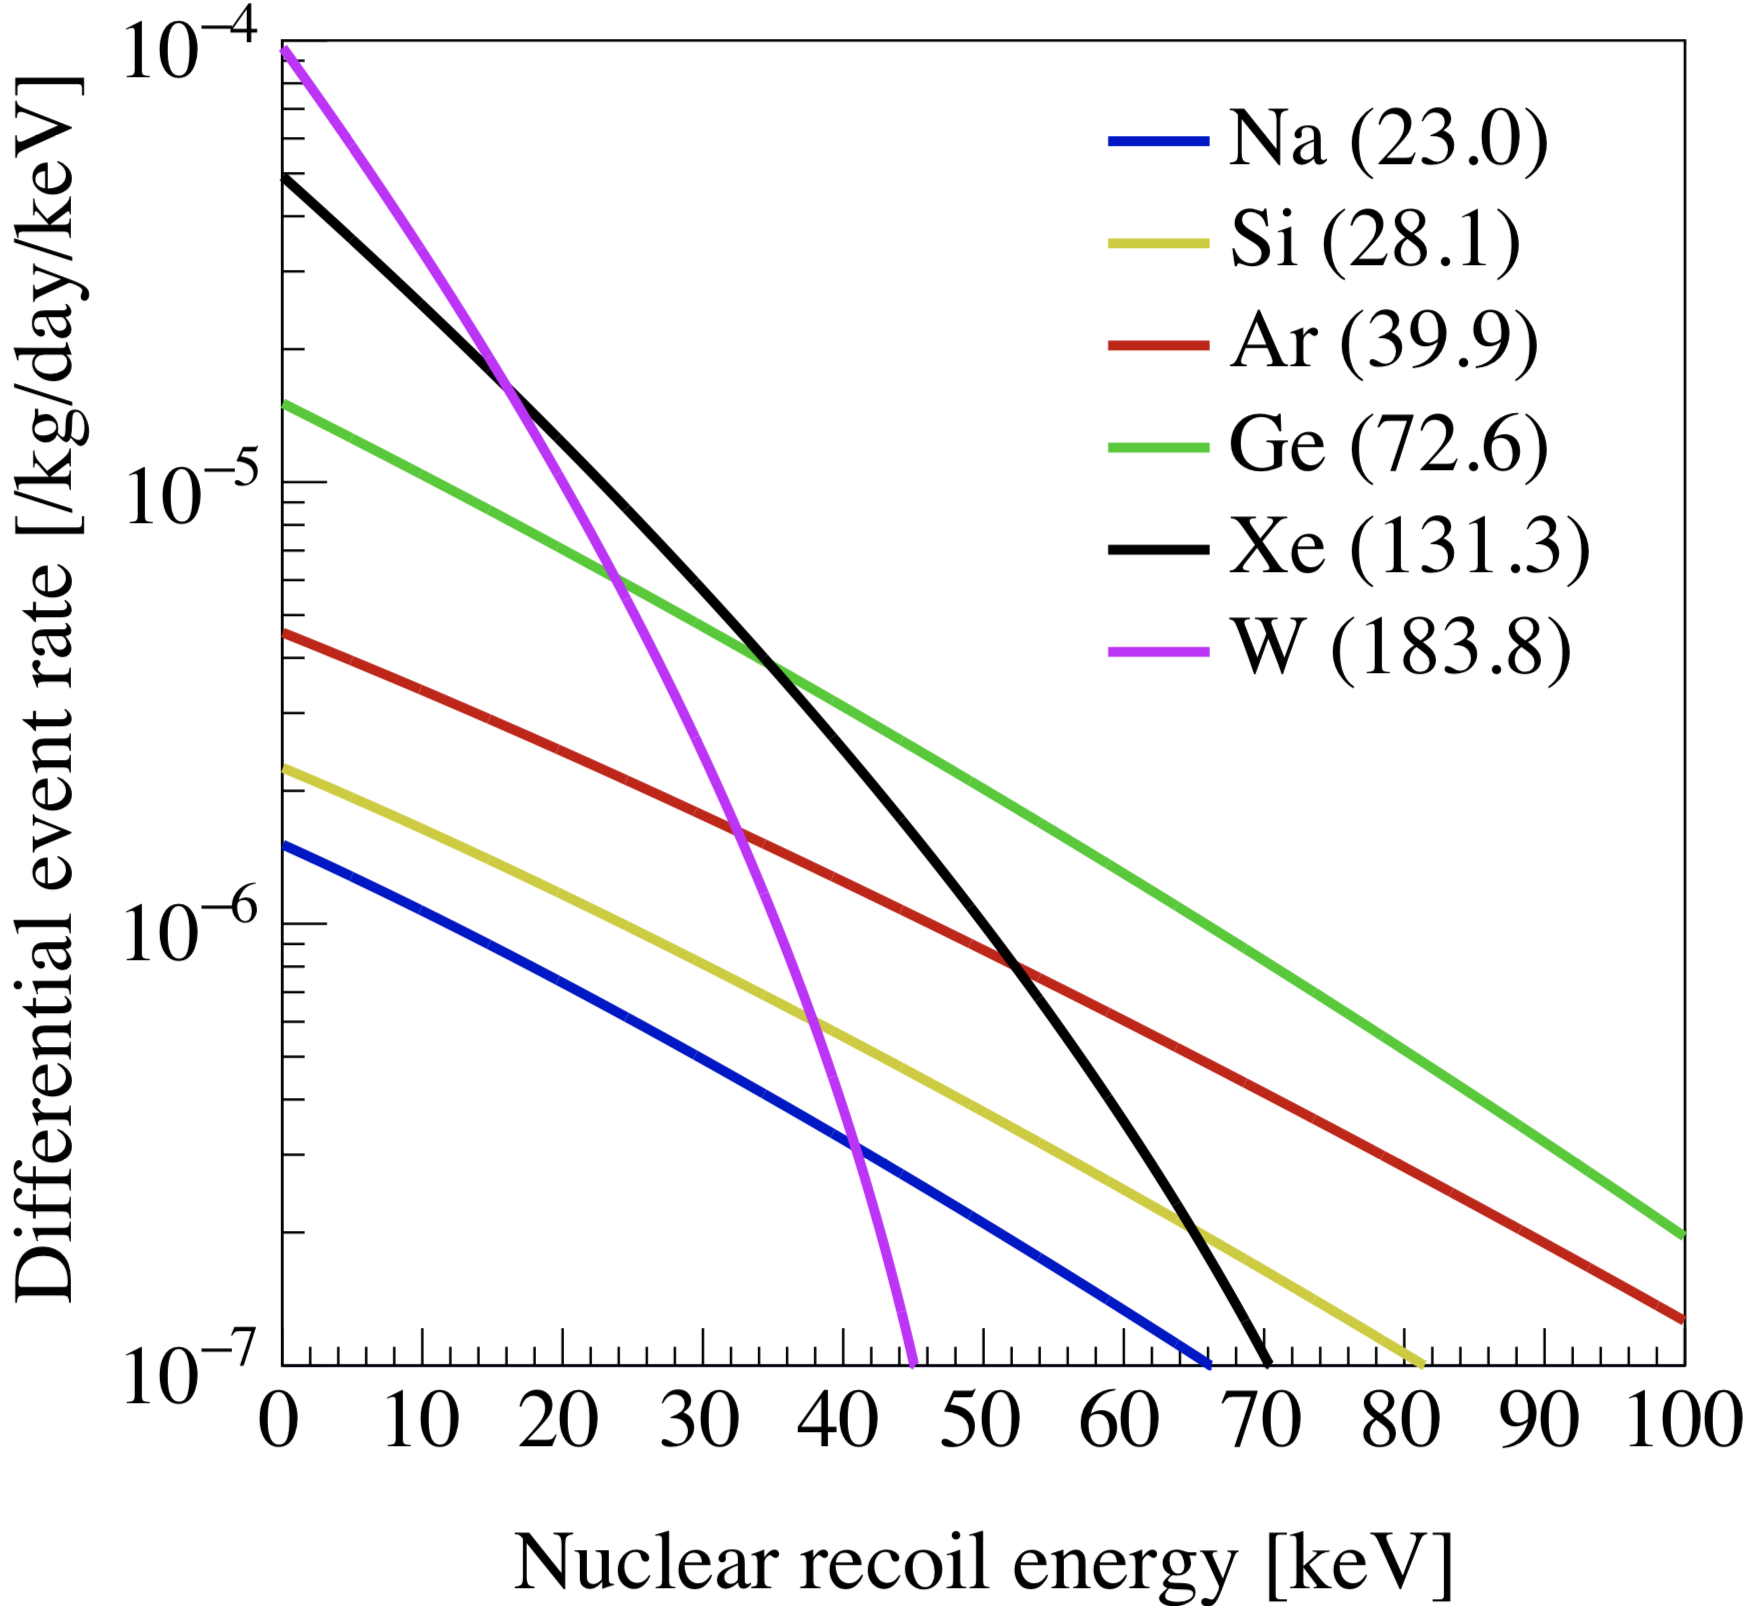
\includegraphics[scale=0.30]{Chapter_2/Figures/SI_nuclear_recoil_rates.png}
        \caption[Comparison of differential event rates of a $100 \; \MathText{GeV/c}^{2}$ WIMP interaction with several different target material, for an assumed cross-section of $\sigma^{SI}_{N} = 1 \; \MathText{zb}$]%
        {Comparison of differential event rates of a $100 \MathText{ GeV/c}^{2}$ WIMP interaction with several different target material with an assumed WIMP-nucleon cross-section of $\sigma^{SI}_{N} = 1 \; \MathText{ zb}$. The averaged atomic mass of each target element at natural abundance is indicated next to its symbol in the legend.}
        \label{fig:nuclear_recoil_rates}
        \end{center}
\end{figure}
%

The interactions taking place inside the TPC generate three types of signals, of which two can be read out by detectors alike. The first of these are the scintillation photons that are produced in the LXe volume via a mechanism that allows these photons to propagate through the liquid and be detected by VUV-sensitive PMTs that cover the top and bottom of the TPC. The interaction also produces ionisation electrons that are drifted upwards via a vertical electric field of several $100 \MathText{ V/cm}$. Once they reach the liquid surface, these electrons are extracted and accelerated through the gaseous phase, producing electroluminescence light, that which is detected by the PMTs. The following sections will cover in detail the mechanisms in which these signals are produced and how they lead to a precise 3D position reconstruction and an effective background discrimination. 


%%------------------------------$$
%%------------------------------$$
\section{Particle Interactions \& Detection in a Dual-Phase Xenon TPC}
\label{sec:xenonphysics}

Interactions of particles inside a xenon TPC result in electron and nuclear recoils. The majority of the backgrounds originating from radioactive isotopes, such as beta or gamma particles interact mostly via electron recoils, leading to a significant ER rate. Neutral particles, such as neutrons or WIMPs are expected to undergo nuclear recoils. Electron recoils are interactions in which the incoming particle interacts with the orbital electrons of the xenon atoms, whereas nuclear recoils are kinetic interactions off of the atomic nucleus. The recoiling particles in both cases deposit their energy through multiple short-ranged interactions, forming a track in which a cascade of interactions take place. The end result of this cascade converts the initial particle energy into scintillation photons, ionisation electrons and atomic motion (heat), latter of which is undetectable by current TPCs. The following sections will discuss in detail the mechanisms of energy transfer and signal production in such interactions.

%%------------------------------$$
\subsection{Primary Energy Transfer}
\label{sec:energy_transfer}

In rare gases, such as xenon and argon, the energy deposited by radiation is expanded into the production of a number of electron-ion pairs, $N_{ion}$, excited atoms, $N_{ex}$, and thermalised free electrons, known as sub-excitation electrons liberated in the ionisation process. The deposited energy, $E_{0}$, can be expressed into ionisation, excitation, and sub-excitation electrons by the use of a Platzman equation \cite{Platzman, xenon_physics}:
%
\begin{equation} \label{eq:e_transfer}
    E_{0} = N_{ion}E_{ion} + N_{ex}E_{ex} + N_{ion}\eta,
\end{equation} 
%
where $E_{ion}$ and $E_{ex}$ are the mean ionisation and excitation energies, $N_{ion}$ and $N_{ex}$ are the number of ionised and excited atoms, and $\eta$ is the mean kinetic energy of ionised electrons. The energy required to produce a single electron-ion pair can be taken as an averaged value, defined as the W-value, where,
%
\begin{equation} \label{eq:w_value}
    W = E_{0}/N_{ion} = E_{ion} + E_{ex}(N_{ex}/N_{ion}) + \eta.
\end{equation} 
%
The average energy loss in ionisation is slightly larger than the ionisation potential or the band gap energy, resulting in the ratio of the W-value to that of ionisation potential or band gap to be 1.6-1.7 \cite{PhysRevA.48.1313}. In general, the W-value is smaller in the liquid phase, and in LXe, in comparison to liquid argon and neon. As a consequence, the ionisation yield in LXe is the highest of all noble liquids.

Although the above equation is believed to apply for electronic recoils, in the case of nuclear recoils, a large fraction of the deposited energy is spent in nuclear collisions, which do not result in either excitations or ionisations. Hence, an additional term may be considered in equation \ref{eq:e_transfer} to account for this loss. The ratio of $N_{ex}/N_{ion}$ has been measured to be $\sim0.2$ for electronic recoils and yields a value of $\sim1$ for nuclear recoils upon fitting to data \cite{xenon_physics, Dahl}. This difference in the initial ratio of exciton and electron-ion production is thought to be the underlying principle of discrimination between electron and nuclear recoils in two-phase TPCs. Further discussion on discrimination will follow in section \ref{subsubsec:recom_disc}.


%%------------------------------$$
\subsection{Primary Scintillation (S1)}
\label{subsec:s1}

The primary scintillation light---often referred to as an S1 signal---is produced via a process known as self-trapping, in which an excited xenon atom ($Xe^{\ast}$) forms a molecular dimer ($Xe^{\ast}_{2}$) with a neighbouring atom; the decay of which produces a VUV photon. Upon initial recoil, there are two distinct processes in particular that lead to S1 light production. The first of these are when an incoming particle creates an excited xenon atom, which leads to the creation and decay of an excited xenon dimer molecule \cite{xenon_physics}:
%
\begin{align} \label{eq:exciton_luminescence}
    &p_{i} + Xe \rightarrow Xe^{\ast} + p_{i}, \\
    &Xe^{\ast} + Xe \rightarrow Xe^{\ast, v}_{2}, \\
    &Xe^{\ast, v}_{2} + Xe \rightarrow Xe^{\ast}_{2} + Xe, \\
    &Xe^{\ast}_{2} \rightarrow  Xe +  Xe + \gamma,
\end{align}
%
where $p_{i}$ is the incoming particle, representative of any of the primary particle candidates present in such detectors, i.e., electrons, gamma rays, neutrons and so on. The superscript $v$ is used to distinguish vibrationally excited states from purely electronic excitation. The de-excitation of a vibrational state is mostly non-radiative but emission of infrared photons are also possible. The process detailed above is often referred to as \textit{exciton luminescence}.

An alternative process to exciton luminescence is \textit{recombination luminescence}. Although the end result of this process is identical to that of the process above, the initial interaction results in an ionised xenon atom, which undergoes recombination:
%
\begin{align} \label{eq:recombination_luminescence}
    &p_{i} + Xe \rightarrow Xe^{+} + p_{i} + e^{-}, \\
    &Xe^{+} + Xe + Xe \rightarrow Xe^{+}_{2} + Xe, \\
    &Xe^{+}_{2} + e^{-} \rightarrow Xe^{\ast\ast} + Xe, \\
    &Xe^{\ast\ast} + Xe \rightarrow Xe^{\ast} + Xe + (heat), \\
    &Xe^{\ast} + Xe \rightarrow Xe^{\ast, v}_{2}, \\
    &Xe^{\ast, v}_{2} + Xe \rightarrow Xe^{\ast}_{2} + Xe, \\
    &Xe^{\ast}_{2} \rightarrow  Xe +  Xe + \gamma.
\end{align}
%
The emission spectrum of the VUV scintillation photons originating from these two processes are similar as they share a common final stage. In a single event, both of these processes contribute in creating the summed S1 pulse---the collection of the VUV photons originating from an interaction site. However, it is important to note that the rate of recombination luminescence is heavily dependent on the initial energy recoil and more importantly, the electric field applied \cite{Dahl}. Application of an electric field serves as a mechanism to drift away any free electrons from the interaction site, hence suppressing recombination luminescence. 

Although there exists a probability for an optical transition of the excited atoms to undergo a transition to the ground state, the collision rates in liquid xenon often result in the formation of strongly bound two-atomic xenon molecules. These molecules are only bound in their excited states and can exist either in a single state, $^{1}\Sigma^{+}_{u}$, or a triplet state, $^{3}\Sigma^{+}_{u}$, thereafter transitioning to the repulsive ground state, $^{1}\Sigma^{+}_{g}$, where the two molecules separate into two neutral xenon atoms and emit a VUV photon centered at $\sim 178 \; \MathText{nm}$ \cite{FUJII2015293}. Thus, there is no re-absorption of the emitted photon, making xenon highly transparent to its own scintillation light---an important feature for a scintillator. The decay time constants of singlet and triplet states are very short, roughly 2.2 ns and 27 ns, respectively \cite{xenon_physics}. But recombination as highlighted in equation \ref{eq:exciton_luminescence} is a slow process and can impact the shape of the S1 pulse by adding a non-exponential third component, besides the fast (singlet decay) and the slow (triplet decay) components. The application of an electric field usually serves to reduce this third component by extracting the free electrons, hence suppressing recombination.

Furthermore, particle interactions at high energies ($\geq{}\MathText{MeV}$), such as $\alpha$-particles, can lead to the emergence of higher order processes that can decrease the number of primary scintillation photons. At these energies, the particle tracks formed due to high linear energy transfer (LET) increases the density of excited xenon atoms, thereby increasing the probability of interaction between two exited atoms. This process often leads to an increase in the ionisation rate in the track via a process called \textit{bi-excitonic quenching} \cite{bi_excitonic}, where
%
\begin{equation} \label{eq:bi-excitonic_quenching}
    Xe^{\ast} + Xe^{\ast} \rightarrow Xe^{+} + Xe + e^{-},
\end{equation} 
%
A similar process dubbed as \textit{penning ionisation} can also take place if a single excited xenon atom has enough energy to ionise a neutral xenon atom from the ground state
\cite{Dahl}, where
%
\begin{equation} \label{eq:bi-excitonic_quenching}
    Xe^{\ast} + Xe \rightarrow Xe^{+} + Xe + e^{-}.
\end{equation} 
%
In such processes, the excited xenon atoms have enough kinetic energy to ionise another atom upon a collision. These processes on average usually lead to the suppression of the summed S1 pulse at higher energy recoils, as the process reduces the probability of exciton luminescence, which often leads to the creation of a VUV photon.


%%------------------------------$$
\subsection{Ionisation \& Secondary Scintillation (S2)}
\label{subsec:s2}

The electrons which escape recombination are drifted up by a vertical electric field, effectively removing the electrons from the interaction site. The drift velocity of the electrons depend on the strength of the applied electric field. For liquid xenon, a field strength of $\sim 1 \; \MathText{kV/cm}$ can lead to a $2.25 \; \MathText{mm/\mu{}m}$ drift velocity. After about $10 \; \MathText{kV/cm}$, this dependence no longer holds and the drift velocity saturates at $\sim2.8 \; \MathText{mm/\mu{}m}$ \cite{e_drift}. An accurate understanding of the drift velocity and hence the applied electric field is important in reconstructing the depth (\textit{z} or the \textit{t} axis) at which the interaction took place, as this is proportional to the time difference between the S1 signal and the S2 signal---or put it another way, the time it takes for the electrons to travel to the surface of the liquid, as depicted in figure \ref{fig:tpc_diagram_cad}.

The ionisation electrons drifting in a TPC will also experience diffusion in all three spacial dimensions. Diffusion taking place across the \textit{x-y} plane dubbed as transverse diffusion, $D_{T}$, and the \textit{z} plane, also known as longitudinal diffusion, $D_{L}$. The transverse diffusion usually has no first-order effect on the shape of the summed S2 pulse, whereas despite being an order of magnitude smaller, where $D_{L}/D_{T} \simeq 0.1$, the longitudinal diffusion in LXe has a critical effect on the S2 shape as it dictates the photon time of arrival at the photo-detectors. Hence modelling this accurately is crucial for realistic simulations of pulses and for the determination of the depth of the interaction.

Furthermore, electronegative molecules such as $O_{2}$, $H_{2}O$ and $N_{2}O$ can dramatically decrease the mobility of drifting electrons. These molecules can capture free electrons and form negative ions with extremely low mobility, resulting in drift velocities of a few mm/s at practical electric fields. The probability of a capture by such species depend on the concentration, the reaction rate constant and the path length of the electron as it drifts towards the anode. These species are usually present in sourced xenon and often outgas from detector material, constantly contaminating the LXe. Hence, the purification of liquefied rare gases to contaminant levels that are \mathcal{O}(ppb) or lower is of great significance, especially for events at lower energies.

In reaching the liquid surface, the electrons have to overcome a potential barrier to be extracted over into the gas phase. This process is energetically unfavourable and hence an electric field of several kV/cm is usually applied between a grid just below and just above the liquid surface. Upon extraction, the electrons are accelerated through the gaseous layer to sufficient energies to excite the gas atoms, thus produce secondary scintillation, also known as \textit{electroluminescence}. This process allows very high amplification gains to be achieved, where signals from a single electron to be detected. The mechanism in which secondary scintillation photons are produced is similar to that explained for primary scintillation. A schematic diagram of a toy TPC, highlighting signal generation from an S1 and an S2 signal is depicted in figure \ref{fig:tpc_diagram_cad}. 
%
\begin{figure}[hb!]
    \begin{center}
        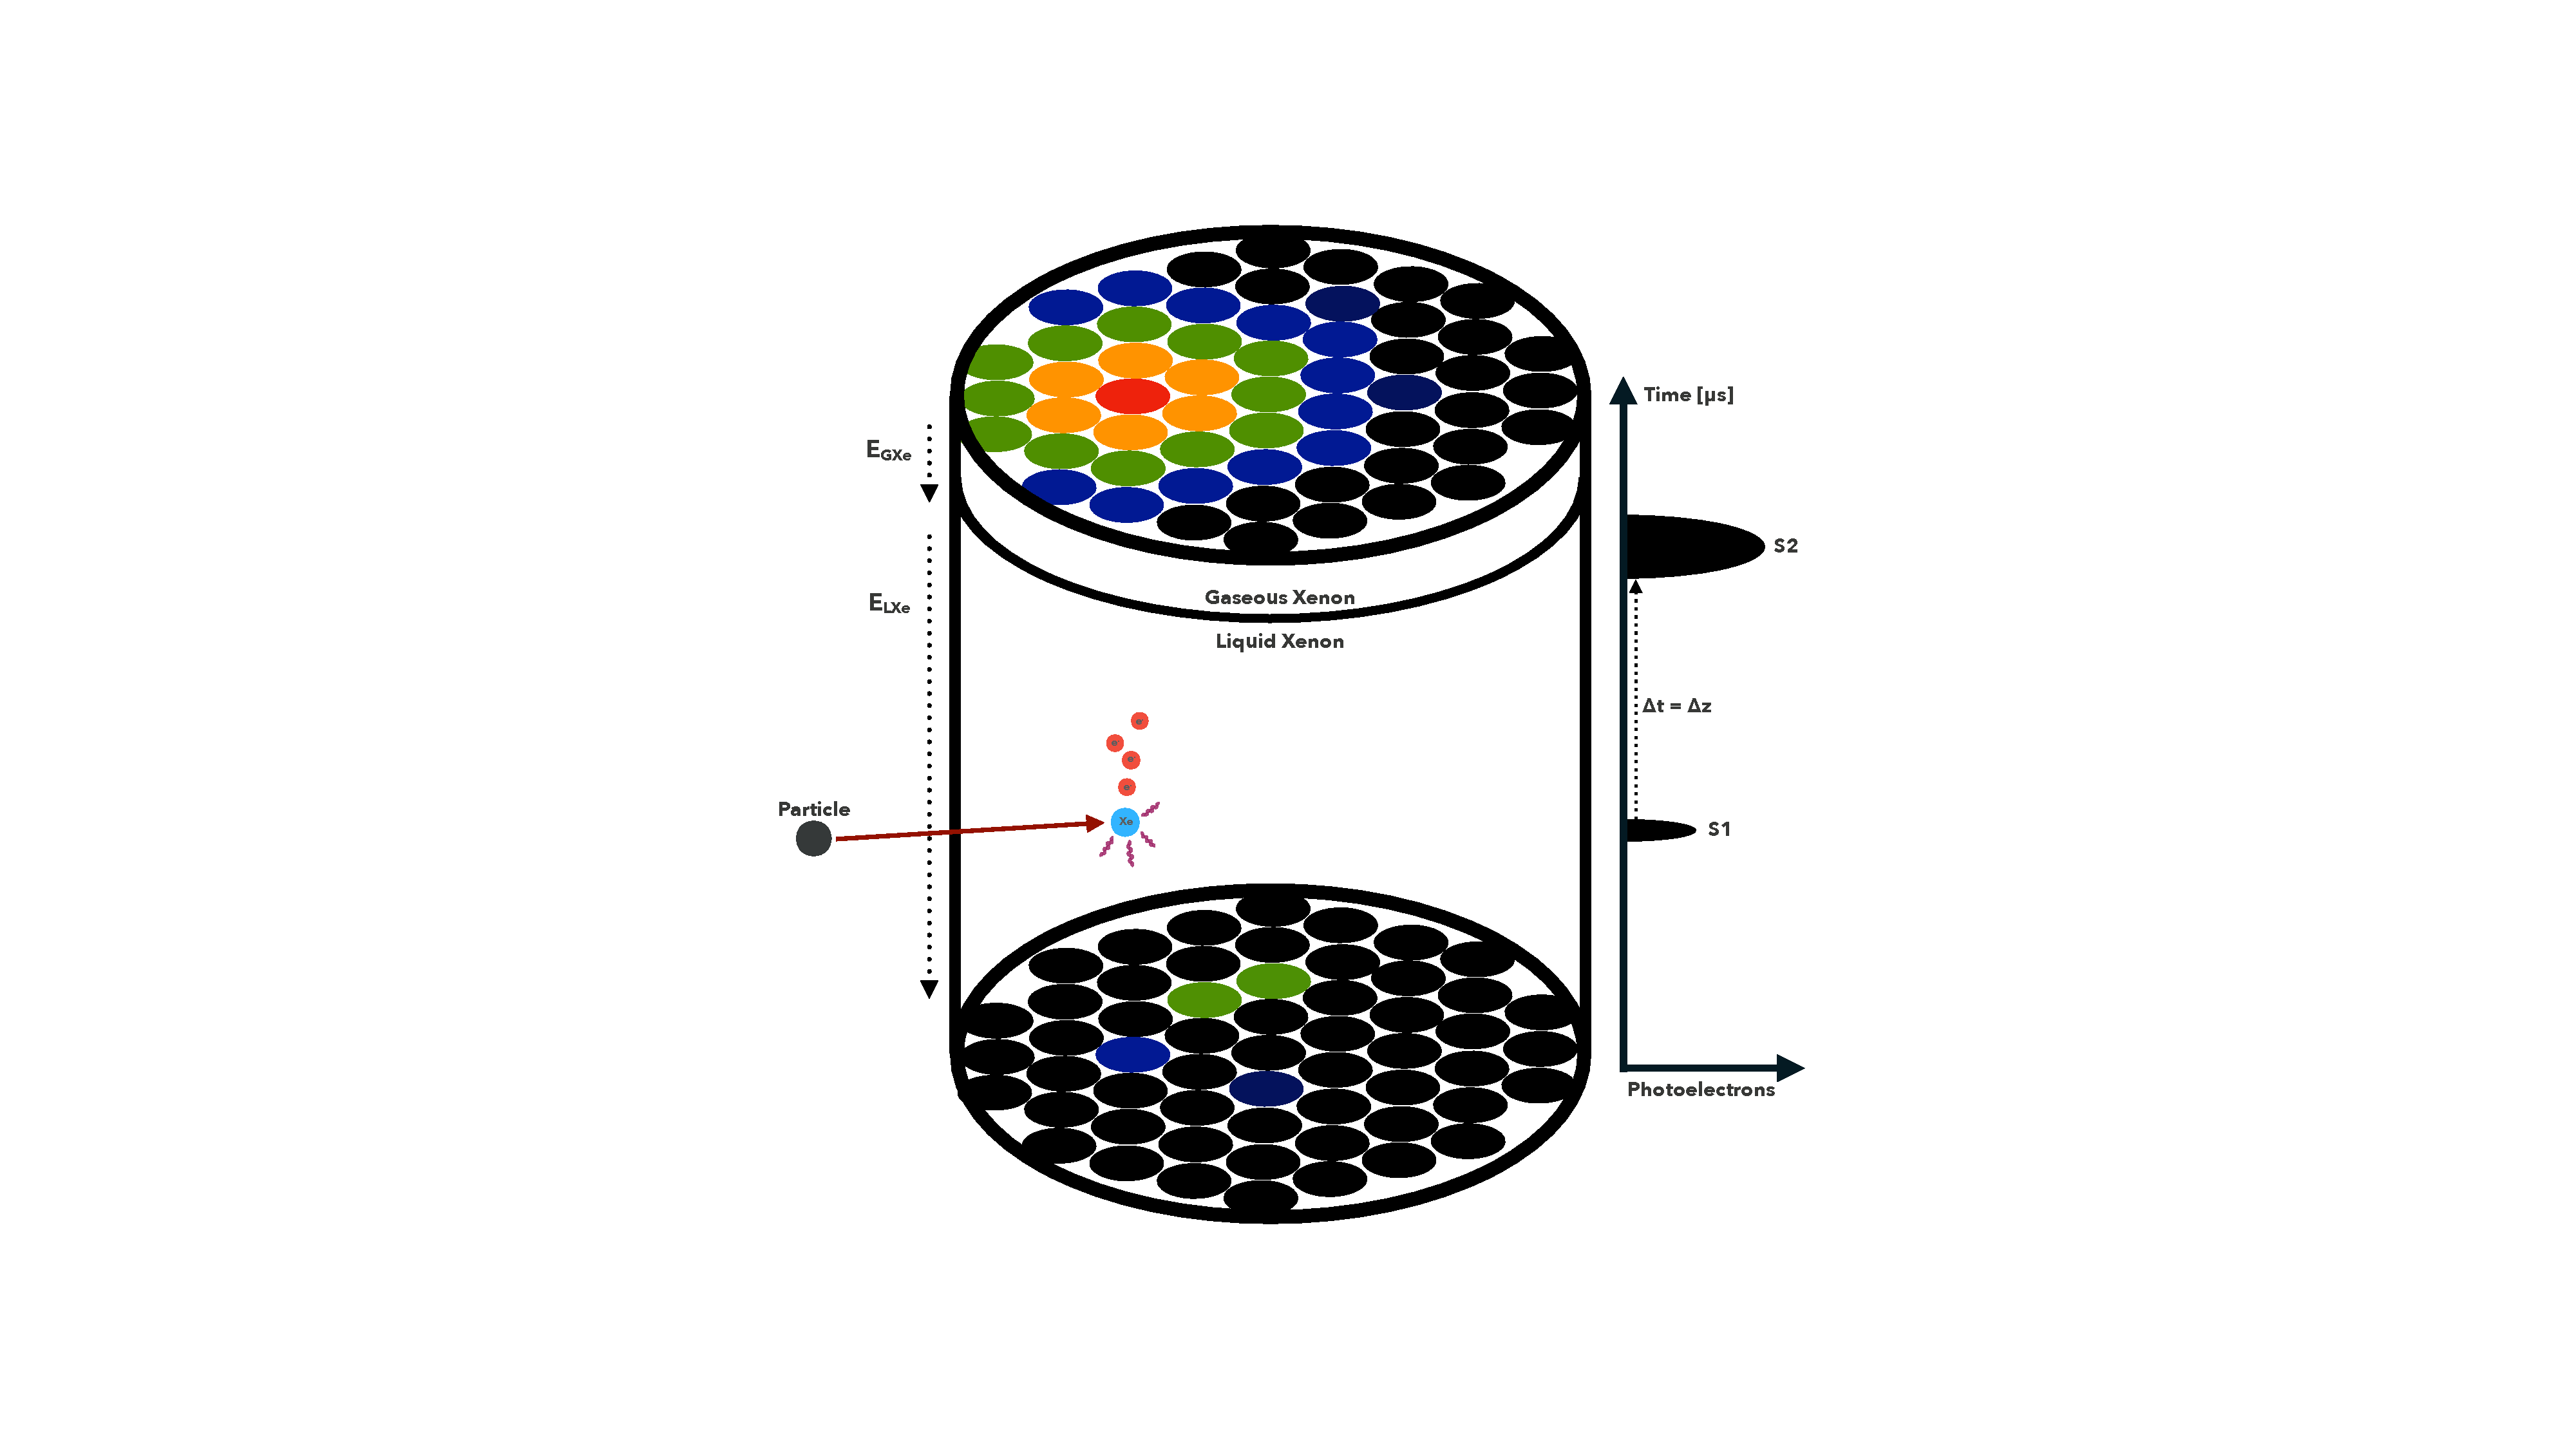
\includegraphics[scale=0.30]{Chapter_2/Figures/TPC_Diagram.pdf}
        \caption[Schematic of a single scatter event inside a dual-phase toy TPC, showing the S1 signal production and the drift of free electrons towards the gas layer]%
        {Schematic of a single scatter event inside a dual-phase toy TPC, showing the S1 signal production and the drift of free electrons towards the gas layer. The top and the bottom of the TPC is covered by PMTs that eventually detect the VUV photons created both in the liquid and in the gas phase. The diagram also depicts how TPCs allows for a 3D position reconstruction; where z is determined by the drift time of electrons and x-y determined by the PMT hit pattern.}
        \label{fig:tpc_diagram_cad}
        \end{center}
\end{figure}
%


%%------------------------------$$
\subsection{Energy Reconstruction and Signal Yields}
\label{sec:energy_recon_signal_yields}

Although the underlying principles that go into S1 and S2 production are relatively trivial, the modelling of these processes and correlating the output signal from a detector to a set of initial conditions depicting reality is less so. Taking into account the above, the number of emitted VUV photons, $n_{\gamma}$, and the escaped electrons, $n_{e}$, from an interaction site after recombination can be expressed as,
%
\begin{equation} \label{eq:photon_electron_recombination}
    &n_{\gamma} = N_{ex} + rN_{ion}, \\
    &n_{e} = (1 - r)N_{ion},
\end{equation}
%
where $N_{ex}$ and $N_{ion}$ are the total number of excited and ionised xenon atoms prior to recombination, respectively, and $r$ is the probability of recombination. In dual-phase TPCs, the detection of scintillation or ionisation due to a particle interaction is observed as an electronic signal that is proportional either to the number of emitted VUV photons, $S1 \propto n_{\gamma}$, or the number of escaped electrons, $S2 \propto n_{e}$. 

On an event-by-event basis, number of excitons, $N_{ex}$, and ionisations, $N_{ion}$, produced, is subject to statistical fluctuations---however, not independently. Therefore reconstructing the energy deposited by using only S1 or S2 light is also subject to the same fluctuations. In realising that, $ n_{\gamma} + n_{e} = N_{ex} + N_{ion}$, for any value of r, and the anti-correlation of S1 and S2 light, a linear combination of S1 and S2 could be used to construct a combined signal to form an improved energy estimator,
%
\begin{equation} \label{eq:combined_energy}
    E_{0} = \mathcal{L}W(n_{\gamma} + n_{e}). 
\end{equation}
%
The W-value in this case represents the average energy required to produce either an exciton or a electron-ion pair, and has an approximated value of 13.7 eV in LXe \cite{Dahl}. $\mathcal{L}$ is referred to as the \textit{quenching factor}, representing the fraction of the recoil energy that is transferred to electronic excitation instead of atomic motion. For electron recoils, this fraction is assumed to be negligible; whereas for nuclear recoils, a large amount of energy is lost as atomic motion. The commonly used model in estimating for this fraction comes from Lindhard’s theory, which is based on heavy ion quasi-elastic collisions and gives the energy dependent nuclear recoil quenching factor as \cite{Lindhard, Lindhard_2},
%
\begin{equation} \label{eq:combined_energy}
    \mathcal{L} = \frac{kg(\epsilon)}{1 + g(\epsilon)},
\end{equation}
%
where $k$ is a constant of proportionality between electronic stopping power and the recoil velocity of the nucleus and $g(\epsilon)$ is a function that models the ratio of electronic-to-nuclear stopping powers. $\mathcal{L}$ is sometimes referred to as the \textit{Lindhard factor} and the energies corresponding to ER or NR events are commonly reported as $keV_{ee}$ and $keV_{nr}$, highlighting the electronic and nuclear recoil equivalent energies.

\subsubsection{Light \& Charge Yields in Liquid Xenon}
\label{subsubsec:light_charge}

In a xenon TPC, where searches are conducted across a wide range of recoil energies, it is often useful to define the light, $L_y$, and charge, $Q_y$, yields, as the number of photons emitted in scintillation or the number of electrons ionised, per keV of recoil energy, respectively, where
%
\begin{equation} \label{eq:combined_energy}
    &L_y = n_{\gamma}/E_{0}, \\
    &Q_y = n_{e}/E_{0}.
\end{equation}
%
The prediction of the liquid xenon yields under the assumed drift electric fields of 180 V/cm and 310 V/cm are presented as the dashed and solid lines in figure \ref{fig:light_charge_yields}. These electric fields are highlighted in particular to represent the fields operated by the LUX experiment and that which the LZ experiment aims to operate under, respectively. The figure also overlays measurements made by the LUX and the PIXeY experiments for both electron and nuclear recoils, down to a few keV of recoil energy, showing a good agreement with the predictions from NEST (Noble Element Simulation Technique) \cite{Szydagis_2011, Mock_2014}. NEST is a simulation package developed as an extension to \textsc{Geant4} \cite{Geant4} to simulate the non-linear behaviour of the energy dependence of scintillation and charge yields as seen by liquid noble detectors. Under its hood, NEST can be seen as a collection of models and approximations that predict the light and charge yields of noble gas elements as a function of recoil energy, electric field, particle type, temperature and pressure. A new version of the \textsc{NEST} software package was released in 2018 (v2.0.0) \cite{nest_v2}, moving away from the initially proposed semi-empirical models, towards a more data-driven approach to match the extensive collection of global data that exists. 

The anti-correlation of light and charge yields for both electron and nuclear recoils are apparent from the solid and dashed \textsc{NEST} lines. The increased recoil energy under a fixed electric field, yields in more ionised electrons, increasing the probability of recombination, and hence increases the light yield. Furthermore, the quanta produced per keV of deposited energy for NR interactions are shown to be quenched across the same energy range. The figure also shows a subtle but noticeable difference between the yields as predicted for 180 V/cm and 310 V/cm; the larger field reduces the recombination probability for both ER and NR events, resulting in a larger charge yield across the energy range.
%
\begin{figure}[hbt!]
    \centering
    \begin{subfigure}
        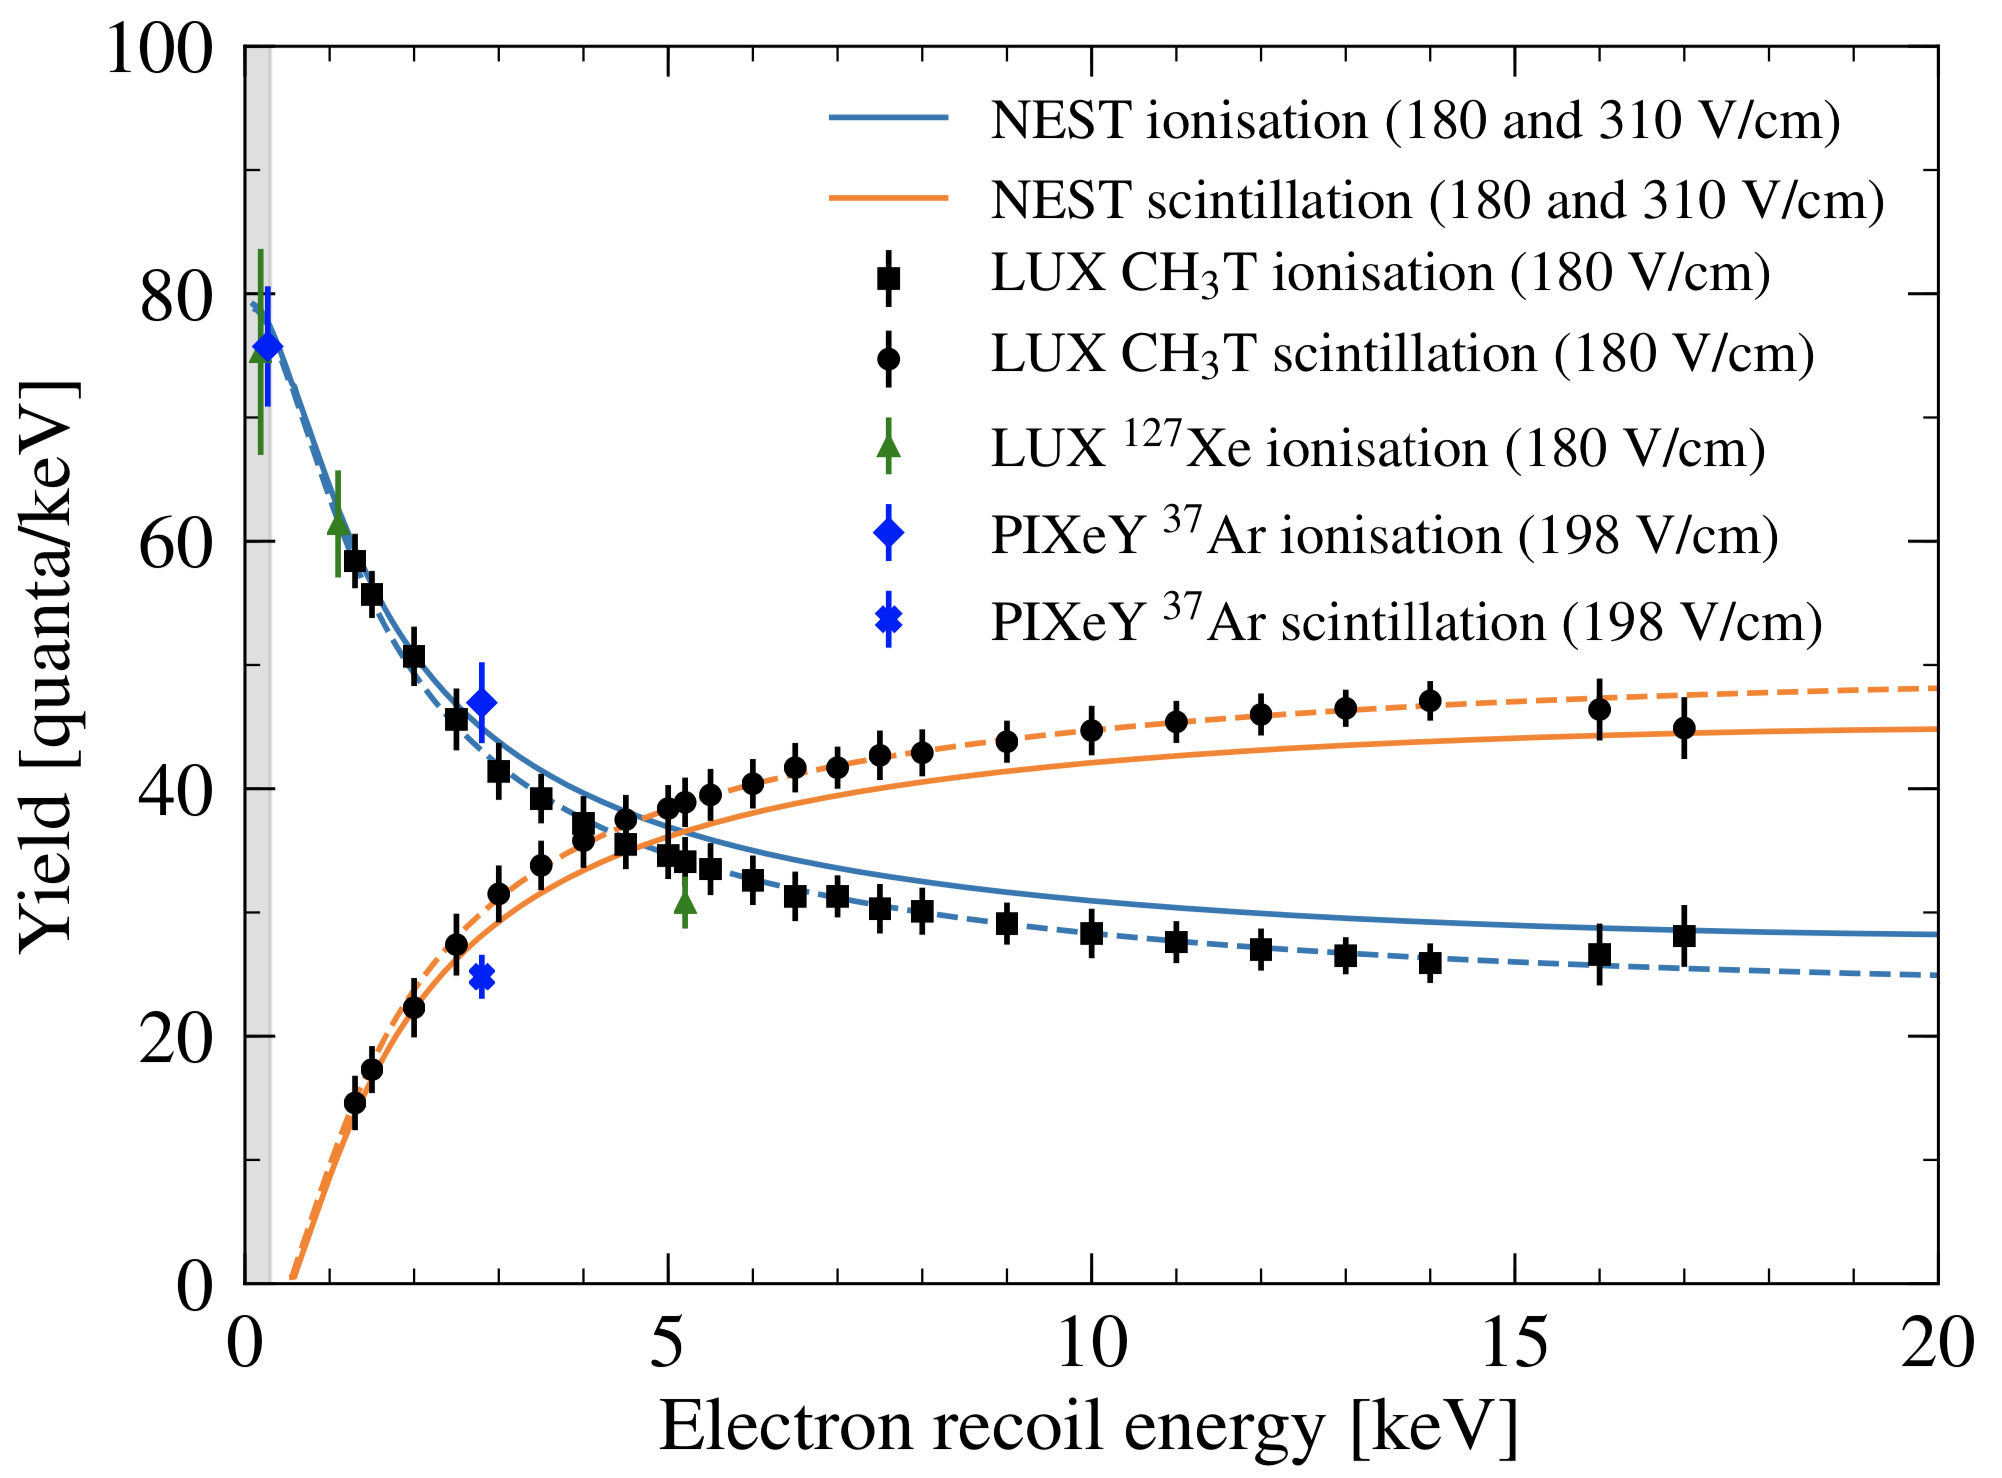
\includegraphics[scale=0.22]{Chapter_2/Figures/electron_recoil_yield.png}
    \end{subfigure}
    \begin{subfigure}
        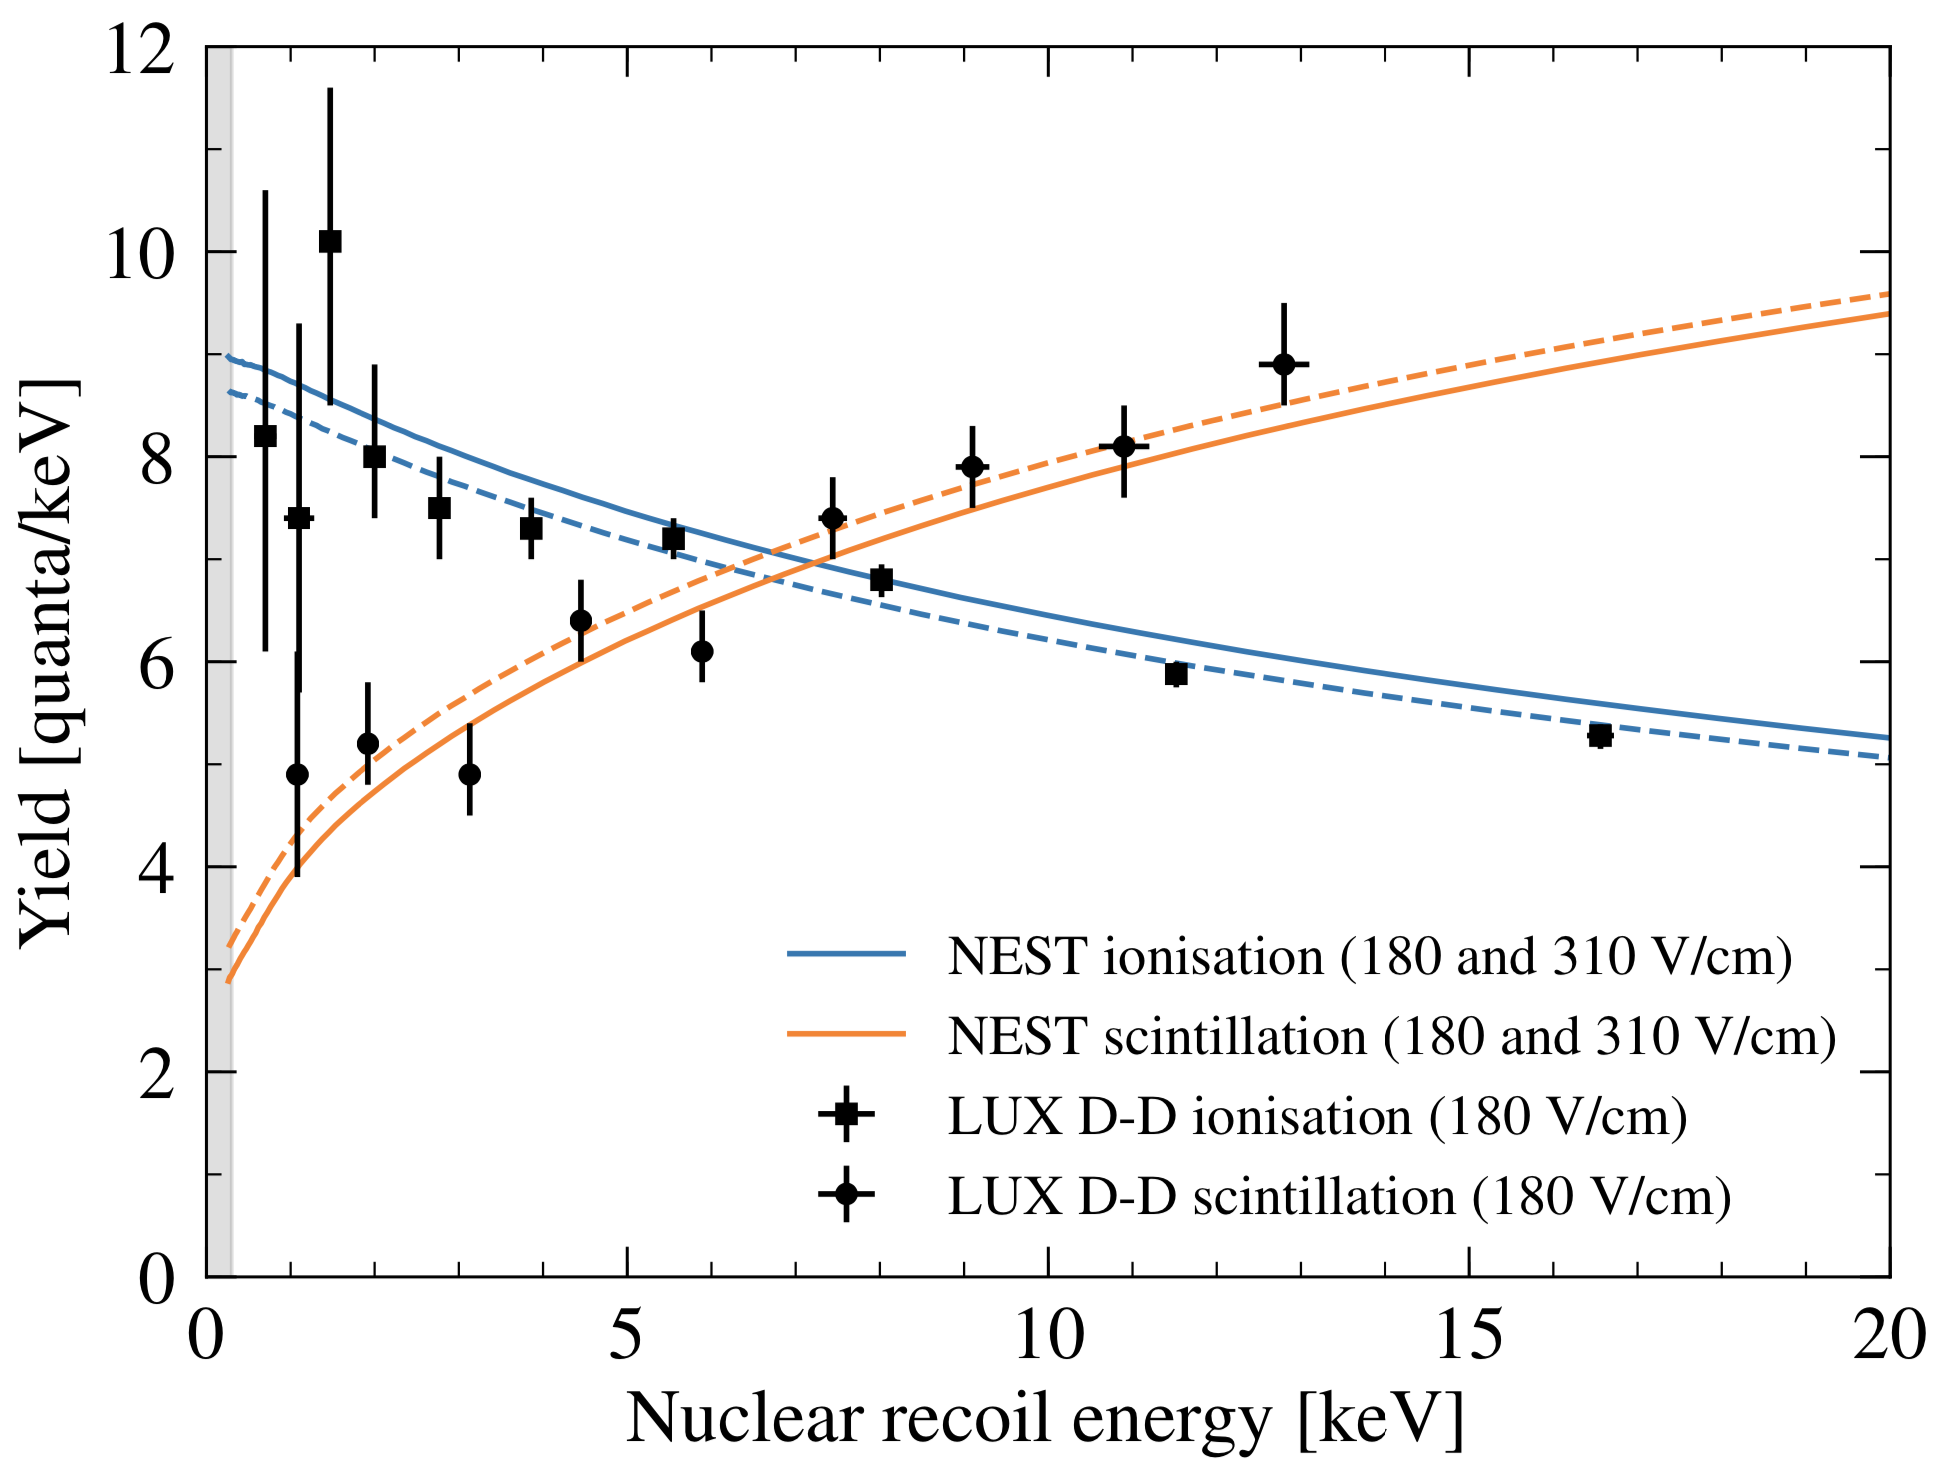
\includegraphics[scale=0.22]{Chapter_2/Figures/nuclear_recoil_yield.png}
    \end{subfigure}
    \vspace*{-5mm}
    \caption[Liquid xenon scintillation and ionisation yields for electron recoils and nuclear recoils.]%
    {Liquid xenon scintillation and ionisation yields for electron recoils (left) and nuclear recoils (right). The NEST prediction of the scintillation and ionisation yields at drift electric field of 180 V/cm (dashed) and 310 V/cm (solid) are represented as the orange and blue lines, respectively. Measurements from LUX CH$_{3}$T \cite{lux_tritium} and $^{127}$Xe \cite{lux_low_energy_cal} calibrations, along with the PIXeY $^{37}$Ar source measurements \cite{PIXeY} are overlaid. Figure adapted from Ref. \cite{ibles}.}
    \label{fig:light_charge_yields}
\end{figure}
%

\subsubsection{Combined Energy Scale}
\label{subsubsec:combined_energy}

The reconstruction of deposited or recoil energy as seen by the detector has to take into account detector specific efficiencies. Upon creation, a single VUV photon will reflect off of surfaces many times, before being successfully recorded by a PMT. The inefficiencies in this process, i.e., absorption of photons upon reflection, the quantum efficiency of PMTs, etc., serves to reduce the overall S1 size. Similarly, inefficiencies for the S2 light is also present, i.e., presence of electronegative molecules, efficiency of extraction into gas phase, etc., reduces the overall S2 size. Therefore, true S1 and S2, as seen by the detector can be defined as,
%
\begin{equation} \label{eq:photon_electron_recombination}
    &S1 = g_{1}n_{\gamma}, \\
    &S2 = g_{2}n_{e}.
\end{equation}
%
Here $g_{1}$ represents the total light collection efficiency in liquid and $g_{2}$ represents the electron detection efficiency, which can be further represented as $g_{2} = n_{e}N_{ph}\epsilon{}g_{1(gas)}$, where $\epsilon{}$ is the electron extraction efficiency, $N_{ph}$ is the number of electroluminescence photons produced per electron, and $g_{1(gas)}$ is the light collection efficiency in the gas phase. By using the combined energy estimator defined in equation \ref{eq:combined_energy}, energy as reconstructed by a detector takes the form,
%
\begin{equation} \label{eq:combined_energy_detector}
    E_{0} = \mathcal{L}W\left(\frac{S1}{g_{1}} + \frac{S2}{g_{2}}\right). 
\end{equation}
%
Both $g_{1}$ and $g_{2}$ can be measured experimentally by the use of known calibration sources, as detailed in \cite{lux_signal_yields} for the LUX experiment. Due to the difference in the quenching factors between ER and NR events, calibration sources using \grays{}, are presented in electron equivalent energies, \kevee{}. As an example of the way these scales work, a \gray{} induced electron recoil of 6 \kevee{} would produce roughly the same total light and charge as a nuclear recoil of a $\sim30$ \kevnr{}.

\subsection{ER \& NR Discrimination}
\label{subsubsec:recom_disc}

As mentioned previously, electron and nuclear recoils tend to appear in different regions of the energy-space, as seen by dual-phase LXe detectors. The conventional way in which events are displayed in such detectors is to plot directly in S1-S2 space. An example of such a plot from the LUX calibration data is shown in figure \ref{fig:er_nr_discrimination} \cite{lux_signal_yields}. When plotting in log$_{10}$(S2/S1) verses S1 space, a clear band structure for ER and NR becomes apparent. The discrimination as seen in this plot is thought to be a consequence of the difference in energy dissipation mechanisms for ER and NR events, as energy is deposited into LXe. To first order, the discrimination originates from the ratio of $N_{ex}/N_{ion}$, where more excitons, for the same energy deposition, are expected to form for a NR than for an ER, hence pushing the NR band lower in the log$_{10}$(S2/S1) axis. The quantification of discrimination for LXe is conventionally taken as the fraction of ER events that leak below the NR mean, divided by the total ER events. Although discrimination varies across S1 or at higher energies, this quantity can be averaged in a desired energy range, i.e. WIMP region of interest. LZ is expected to reach an ER-NR discrimination of 99.5\%.
%
\begin{figure}[ht!]
    \begin{center}
        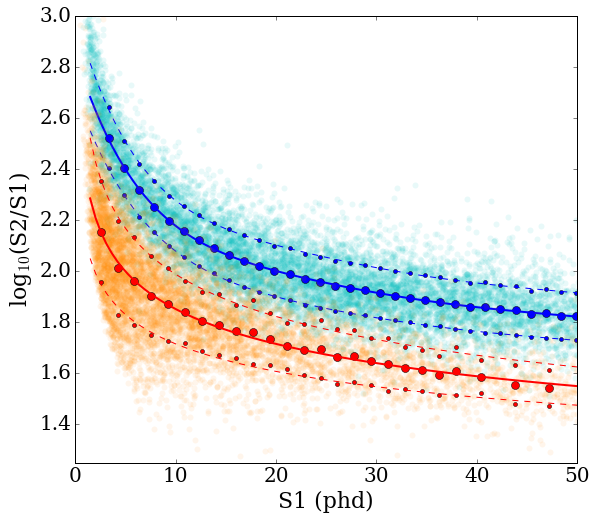
\includegraphics[scale=0.60]{Chapter_2/Figures/PAPER_logS2S1_ERNRBandData.png}
        \caption[Calibration data from the LUX experiment, highlighting the ER and NR band formations in the S1-S2 energy-space.]%
        {Calibration data from the LUX experiment, highlighting the ER and NR band formation (cyan and orange, respectively) in the S1-S2 space. Large filled circles show the fitted band Gaussian mean and small filled circles indicate the fitted Gaussian $\pm1\sigma$. Power law fits to the means and $\pm1\sigma$ are shown with solid and dashed lines \cite{lux_signal_yields}.}
        \label{fig:er_nr_discrimination}
    \end{center}
\end{figure}
%


%%------------------------------$$
\section{The LUX-ZEPLIN Experiment}
\label{sec:lz_detector}

The LUX-ZEPLIN dark matter experiment is housed in the Sanford Underground Research Facility (SURF) in Lead, South Dakota, USA. The detector design is inspired from the LUX and ZEPLIN---III experiments that independently operated dual-phase LXe detectors at much smaller scales \cite{LUX_experiment, zeplin3}. In search for WIMP dark matter, the LZ detector at its core will operate a dual-phase xenon TPC with an active mass of 7 tonnes. To achieve optimal sensitivity, the detector is placed 4850 feet underground inside a water tank; shielded from cosmogenic and atmospheric backgrounds. In operating a LXe skin veto system (dubbed as the skin veto) that surrounds the TPC, and additionally, an outer veto system---dubbed as the outer detector (OD), which utilizes a gadolinium-loaded liquid scintillator (GdLS), the LZ experiment is projected to exclude spin-independent WIMP-nucleon cross sections above $1.4 \times 10^{-48} \; \MathText{cm}^{2}$ for a $40 \; \MathText{GeV/c}^{2}$ WIMP mass at a 90\% confidence level \cite{akerib2018projected}. The following sections will detail the experimental design of LZ, highlighting key operational elements in its search for dark matter, some of which are displayed in figure \ref{fig:cross_sectional_LZ}.

%
\begin{figure}[ht!]
    \begin{center}
        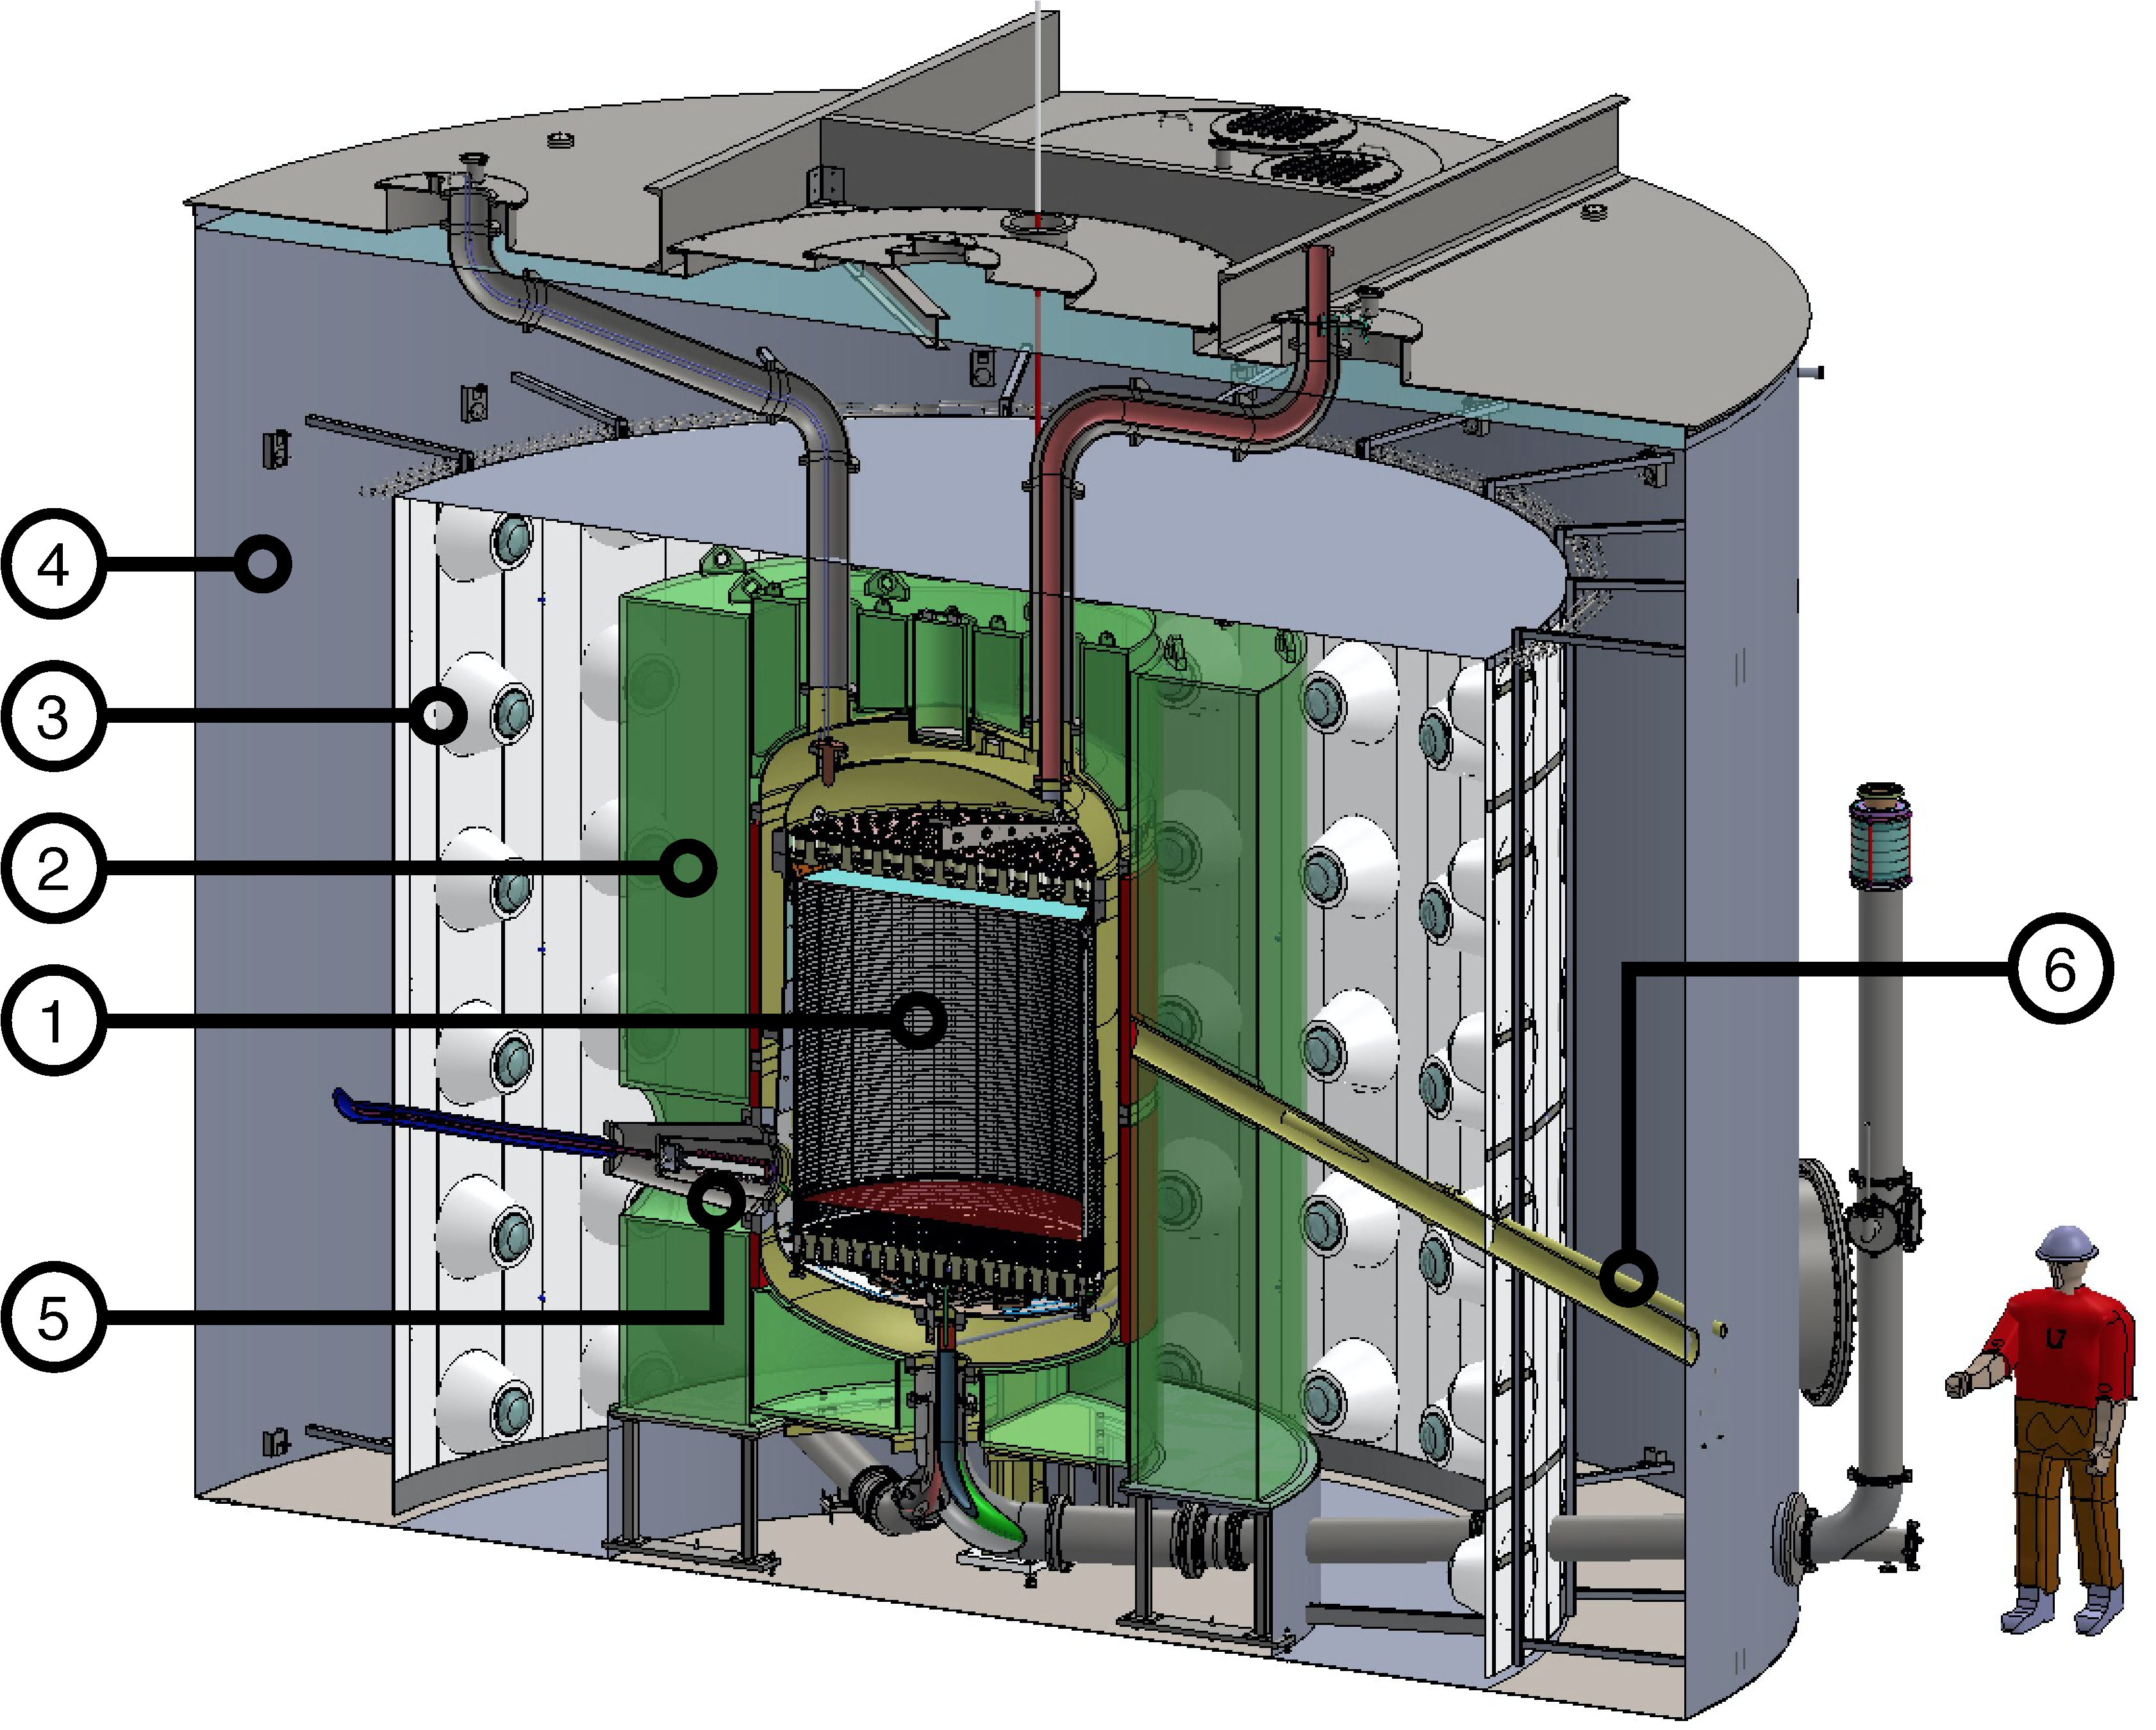
\includegraphics[scale=0.18]{Chapter_2/Figures/LZ_detector_cross_section.pdf}
        \caption[Cross-sectional CAD model of the LZ experiment, highlighting the major detector subsystems.]%
        {Cross-sectional cad model of the LZ experiment, highlighting the major detector subsystems. The LXe TPC (1) is located at the center with PMT arrays covering the top and the bottom. The TPC is sealed within a double-walled vacuum-insulated titanium cryostat that is surrounded by gadolinium-loaded liquid scintillator (GdLS) outer detector (2), surrounded by a suite of 8" PMTs (3) inside the water tank (4). The cathode high voltage (5) and the neutron calibration source conduit (6) are also depicted \cite{Akerib:2019fml}.}
        \label{fig:cross_sectional_LZ}
        \end{center}
\end{figure}
%

\subsection{Liquid Xenon TPC \& Skin Detector}
\label{subsec:tpc_skin}}

The xenon detectors operated by LZ are housed in a double-walled vacuum-insulated titanium cryostat. The inner cryostat vessel (ICV) contains within it the TPC and the skin region. In operation, LZ handles a total of 10 tonnes of liquid xenon; 7 tonnes held inside the TPC and an additional $\sim2$ tonnes held in the skin region. The TPC volume is usually referred to as the active volume which constitutes the WIMP target, and the skin volume refers to the region between the inner cryostat vessel and the outer surface of the TPC---both of which are instrumented with PMTs. 

The TPC volume measures approximately 1.5 m in diameter and height, with a primary objective of detecting S1 and S2 light that are produced both in the liquid and the gaseous layers of this volume. To optimise the collection efficiency of S1 light, the TPC walls as seen by the photons are coated by highly reflective PTFE with a reflectivity of $\geq97.3\%$ when immersed in LXe \cite{Neves_2017}. The S2 electrons produced within the liquid are handled by the operation of four horizontal electrode grids, woven from stainless steel wires, splitting the TPC into three different regions of electric field.

The drift field region (DFR) with a length of 145.6 cm extends from the cathode grid at the bottom of the detector, to the gate grid, located just below the liquid surface, and is shaped by 58 equally spaced titanium field-shaping rings that are embedded into the PTFE panels of the TPC wall. The DFR provides a vertical drift field for ionised free electrons to drift to the liquid surface. The extraction field region (EFR), also known as the electroluminescence region, is located between the gate (5mm below liquid surface) and the anode (8 mm into the gas). Electrons drifted to the surface of the liquid are extracted by this region and accelerated through the gas layer to generate $\sim$820 electroluminescence photons per electron, of which the S2 light is constructed. The final region, known as the reverse field region (RFR) is located between cathode and another grid that sits just below. This space uses 8 field-shaping rings and serves to protect the bottom PMT array from the high potential of the cathode grid, while also drifting the electrons created in this region downwards, hence removing the S2 signal from events occurring below the cathode. A diagram of the TPC with key highlights are shown in figure \ref{fig:tpc_diagram}.

%
\afterpage{
    \begin{figure}[h!]
        \centering
        \begin{subfigure}
            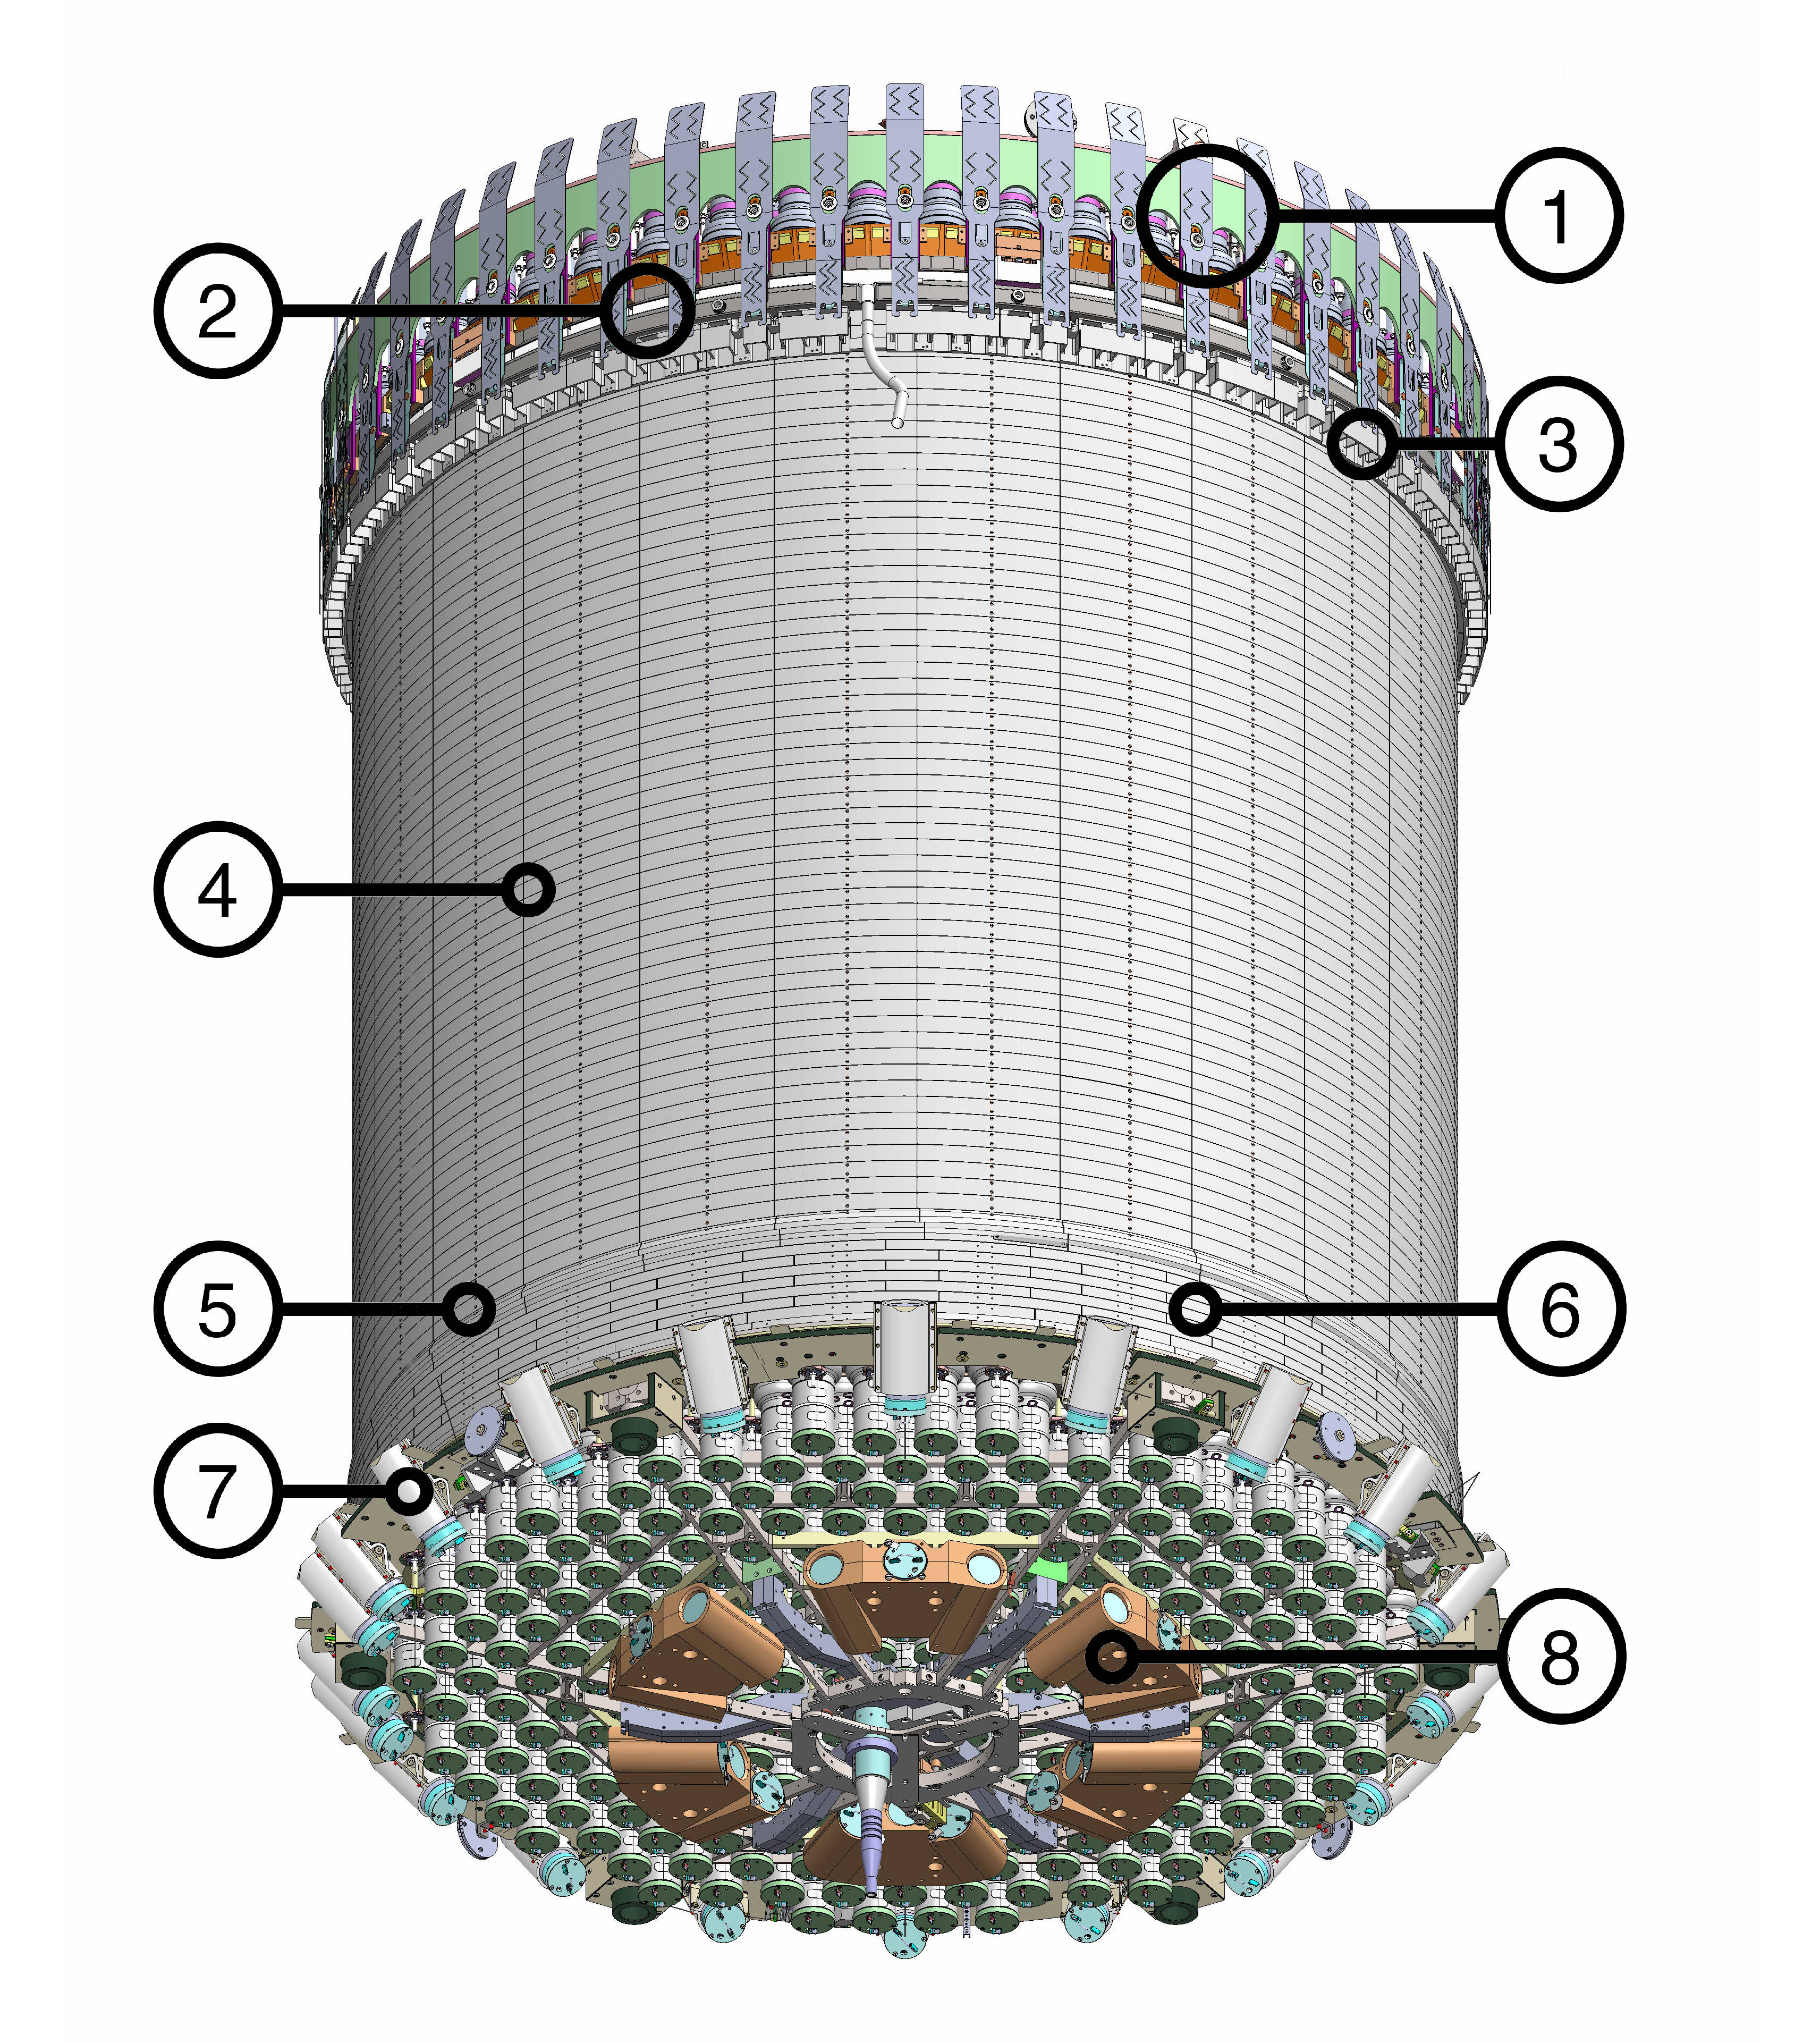
\includegraphics[scale=0.60]{Chapter_2/Figures/TPC_CAD_reduced.jpg}
        \end{subfigure}
        \hspace*{10mm}
        \begin{subfigure}
            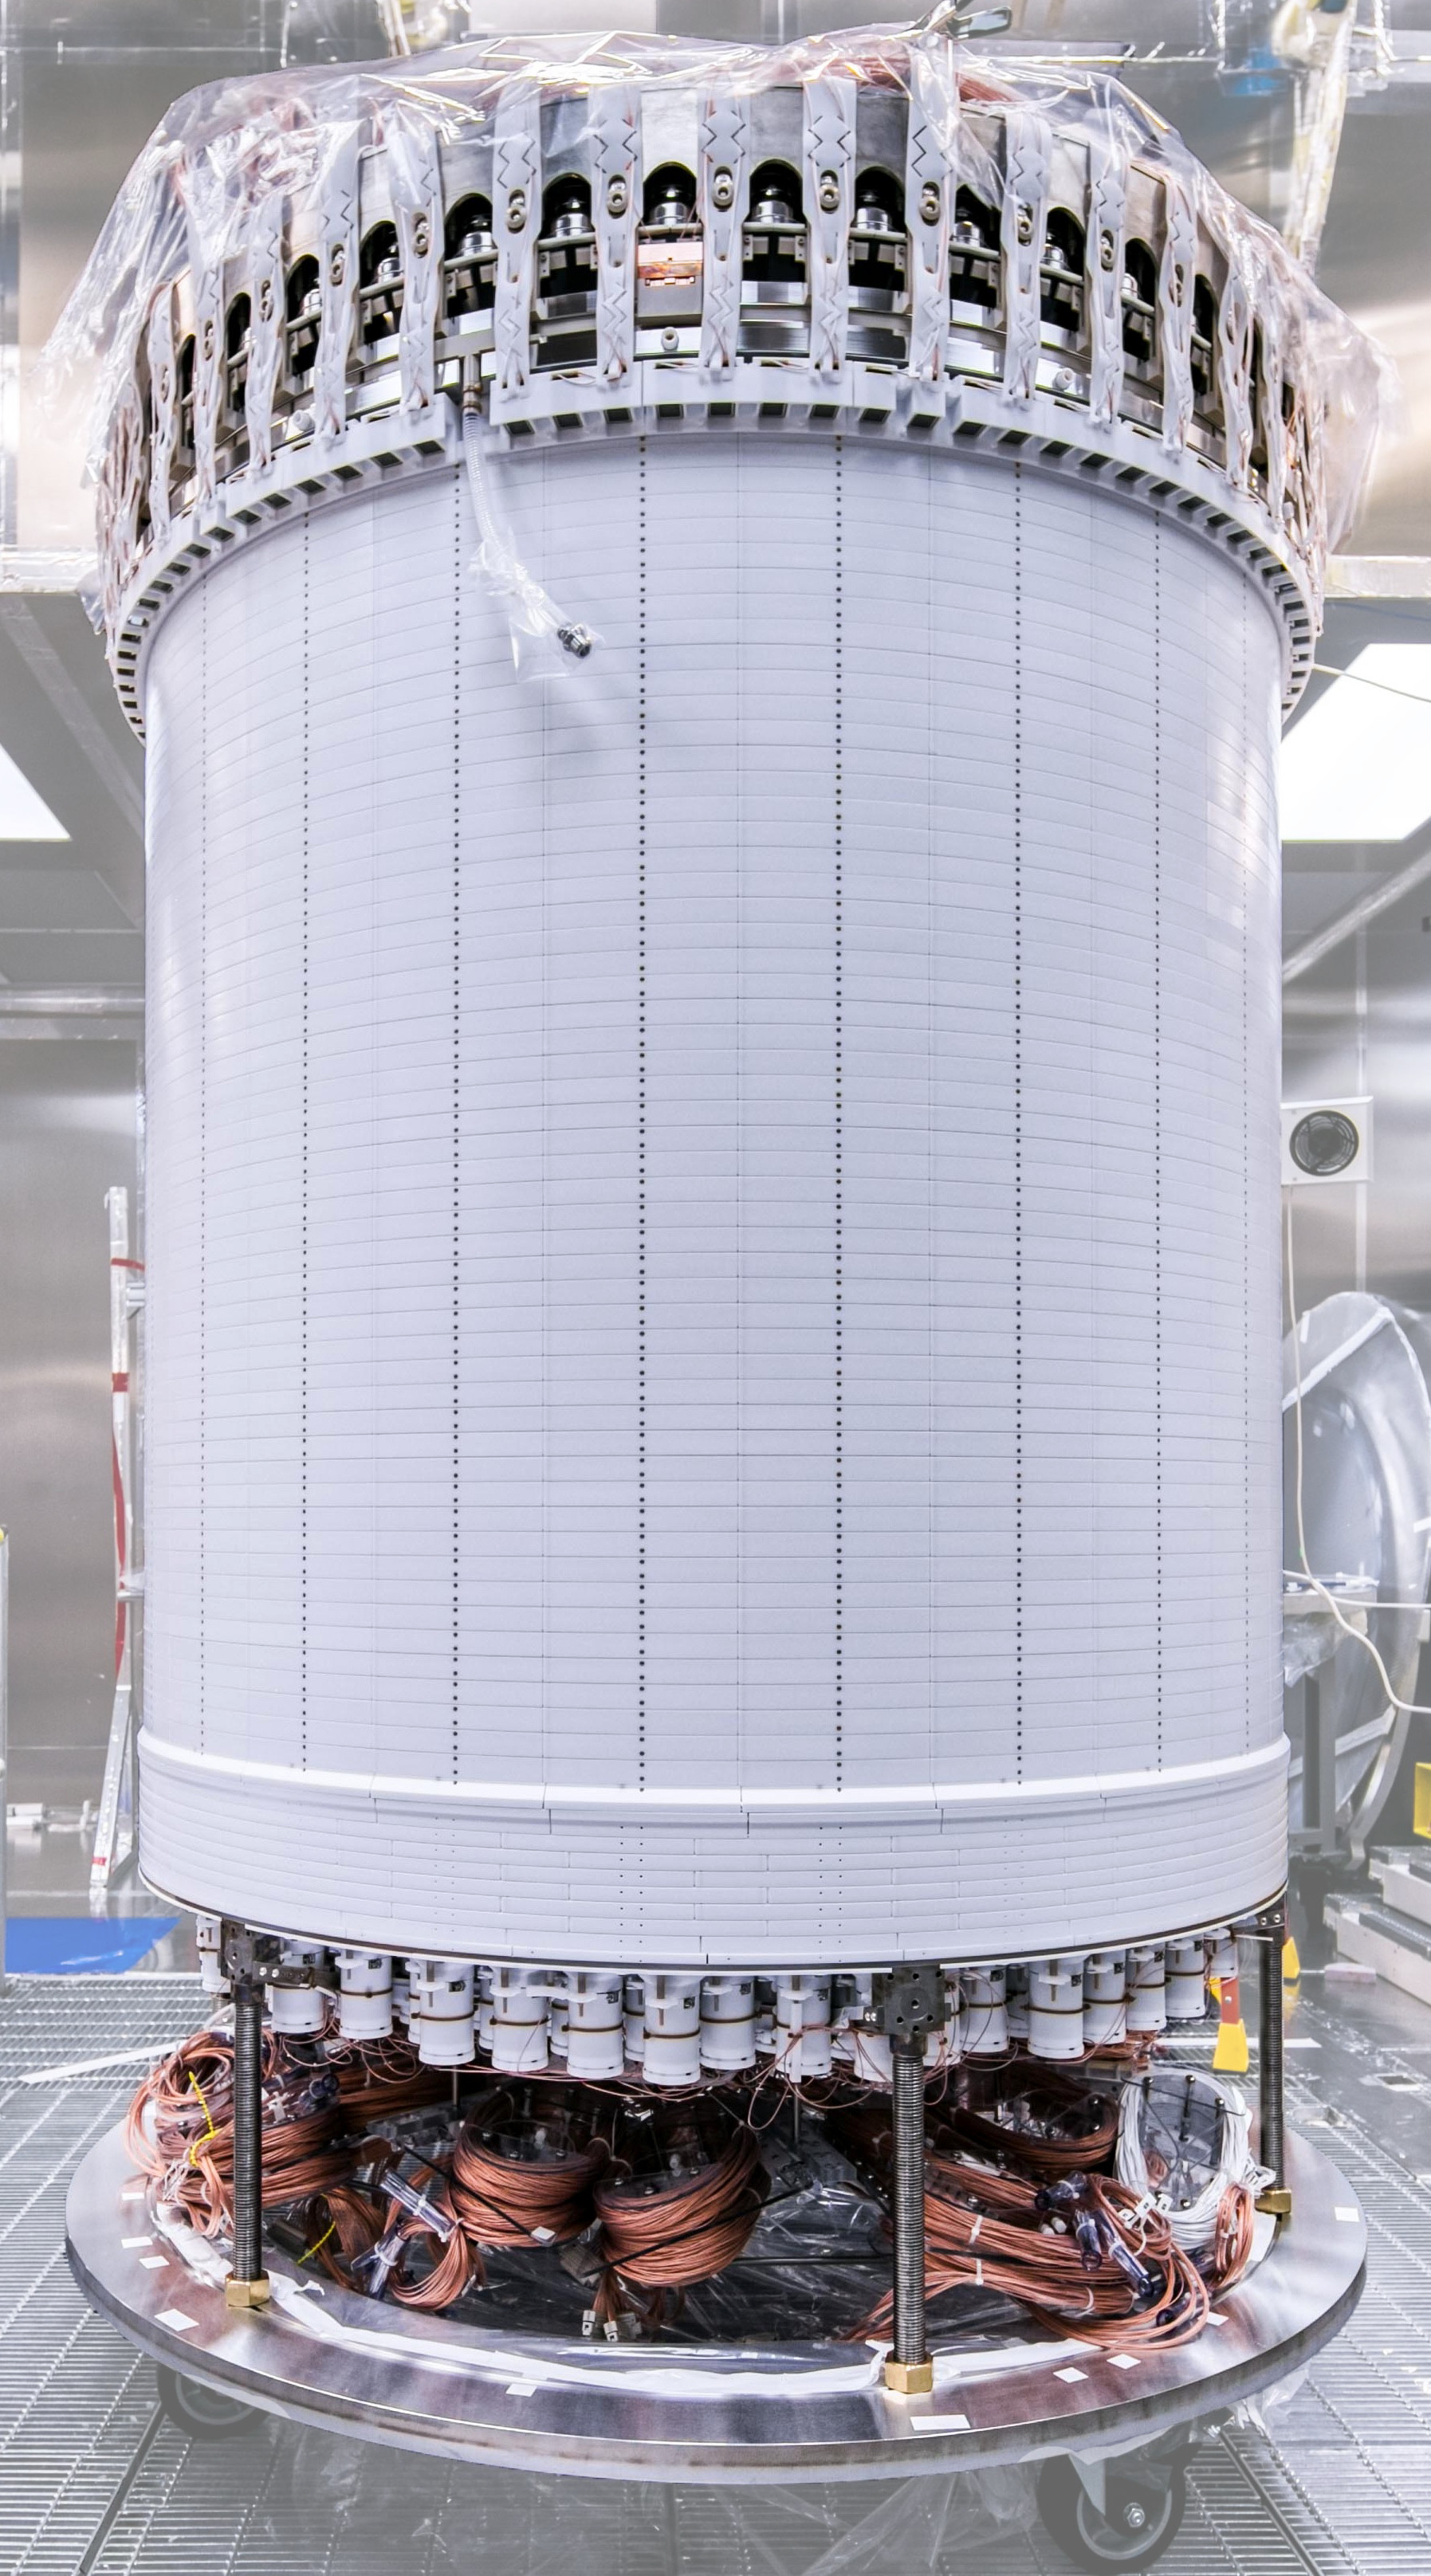
\includegraphics[scale=0.28]{Chapter_2/Figures/TPC_real_reduced.jpg}
        \end{subfigure}
        \caption[A diagram showing the CAD (left) and the fully constructed TPC (right), detailing the key components of the system.]%
        {A diagram showing the CAD (left) and the fully constructed TPC (right), detailing the key components of the system. 1- Top PMT array; 2-Gate-anode and weir region (liquid level); 3-Side skin PMTs (1-inch); 4-Field cage; 5-Cathode ring; 6-Reverse field region; 7-Lower side skin PMTs (2-inch); 8-Dome skin PMTs (2-inch). Photographed by Matthew Kapust, Sanford Underground Research Facility \cite{Akerib:2019fml}.}
        \label{fig:tpc_diagram}
    \end{figure}
    \begin{figure}[h!]
        \centering
        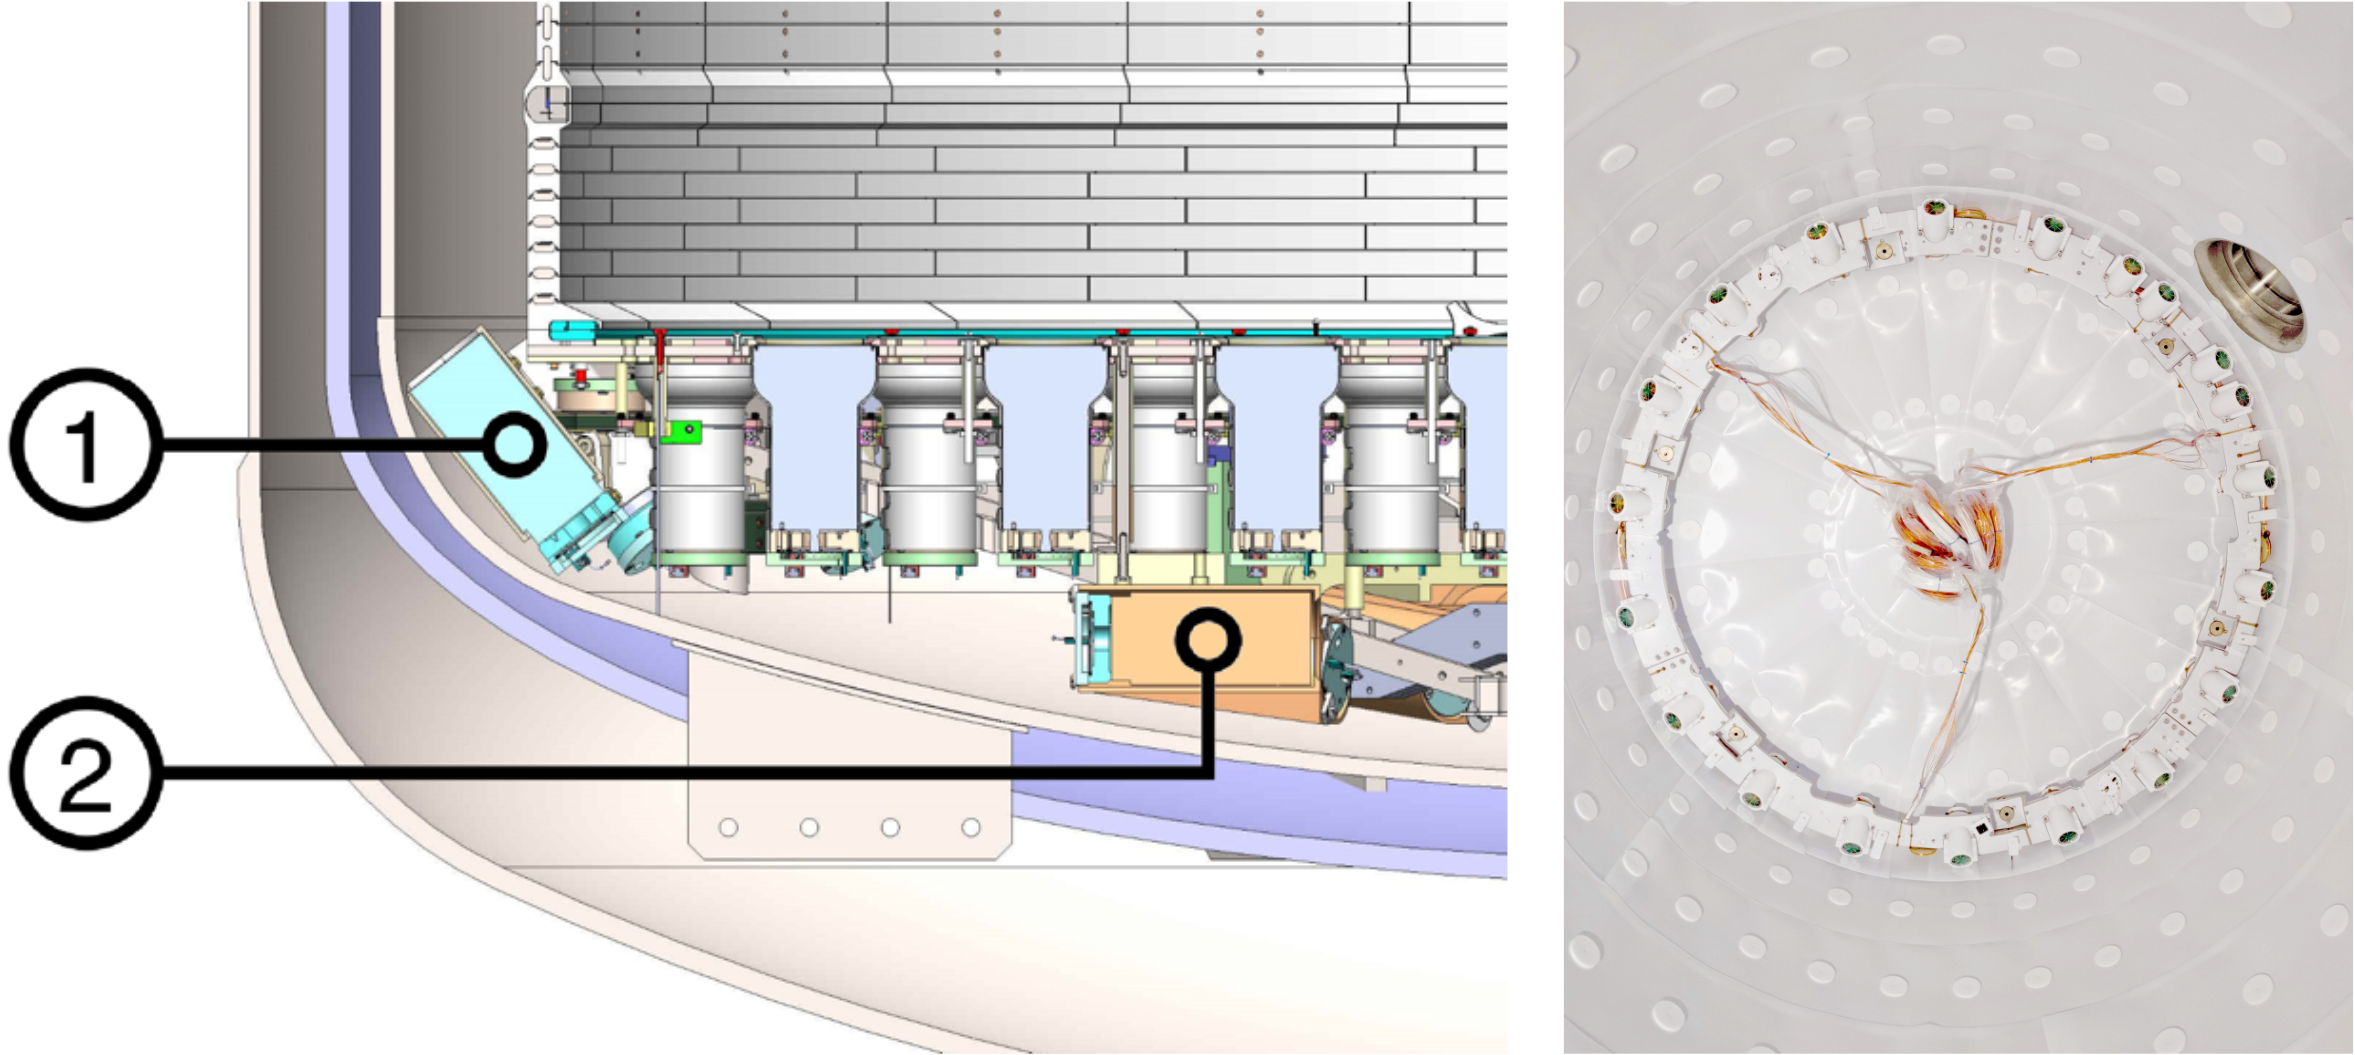
\includegraphics[scale=0.77]{Chapter_2/Figures/Skin_detector.png}
        \caption[CAD diagram (left) showing the TPC below the cathode and a photograph (right), showing the PTFE panelling and the bottom skin PMT array.]%
        {Left: CAD section of the TPC below the cathode showing the location of the 2” bottom side skin (1) and lower dome (2) PMTs. Right: Photograph showing the inner ICV with PTFE panelling on the walls and the lower side skin PMT structure at the bottom of the vessel \cite{Akerib:2019fml}.}
        \label{fig:skin_detector_diagram}
    \end{figure}
}
%

The active volume of the TPC is monitored by two arrays of PMTs. A total of 494 PMTs are divided between the top array with 253 PMTs, and the bottom array with 241 PMTs, respectively. The 3-inch PMTs (model No. R11410-22) were manufactured by Hamamatsu for operation in cold liquid xenon. Furthermore, they were optimised for the detection of VUV luminescence, with an average quantum efficiency of 30.9\% while operating in liquid xenon temperatures, and for low-radioactivity, an excellent single photo-electron (SPE) resolution, and low dark noise. At an operating voltage of 1500 V and 12 dynode stages, a nominal gain of $3.5 \times 10^{6}$ is expected at the end of the signal cable. The PMTs are arranged in close-packed hexagonal patterns to maximise the photocathode coverage and position reconstruction of the S2 signal for interactions near the TPC wall. The array structures are made from low-background titanium sourced as part of the R\&D efforts for LZ \cite{LZ_titanium_selection}. The exposed titanium between the PMTs are covered by interlocking PTFE pieces to maximise VUV reflectance. 

The skin region, sitting outside of the TPC is an important component of the xenon detector. The primary purpose of this region is to serve as a dielectric insulation between the TPC and the ICV. In addition to this, this region is also instrumented with VUV sensitive PMTs to serve as a scintillation-only veto detector, highly effective for \grays{}. The skin veto is composed of two regions: the outer layer of xenon outside of the TPC known as the skin, and the region below the TPC, known as the dome. The skin is monitored by three sets of Hamamatsu PMTs. First of these are a ring of 93 1-inch PMTs (model No. R8520) located at the top of the TPC looking down into the skin, and a further 20 2-inch PMTs (model No. R8778) located at the bottom of the TPC looking up and 18 2-inch PMTs mounted right below the TPC looking into the dome. A schematic of this region is shown in figure \ref{fig:skin_detector_diagram}.


\subsection{Cryogenics \& Xenon Handling}
\label{subsec:crypo_xenon}}

The LZ cryogenic system is designed to contain $\sim$10 tonnes of LXe at 175 K. The xenon detector and majority of the LXe payload is held inside the ICV, 
and vacuum coated with the outer cryostat vessel (OCV). The OCV is supported at the bottom by three legs and the ICV is suspended from the top head of the OCV with a mechanism enabling its levelling from above. The cryostat vessels are fabricated from commercially available pure grade-1 titanium, chosen after an extensive screening campaign to identify the most radio-pure sample within a series of samples taken from different manufacturers, as detailed in \cite{LZ_titanium_selection}.

The ICV consists of a top head and a tapered bottom vessel, connected via a large flange near the top. Its tapered shape is to reduce the electric field near the cathode. The top and the bottom heads of the ICV contain ports for cabling and heat exchancer conduits, with a larger port sitting on the front of the vessel for the high voltage (HV) conduit connection. Whilst the size of the ICV is constrained by the Yates shaft, the OCV is constructed of three segments to overcome this restriction. Similarly, the OCV contains a HV port that aligns with the HV port of the ICV. Furthermore, the OCV also has a port opening to accommodate for the deployment of low energy neutrons that's crucial for calibration.

%
\begin{figure}[b!]
    \centering
    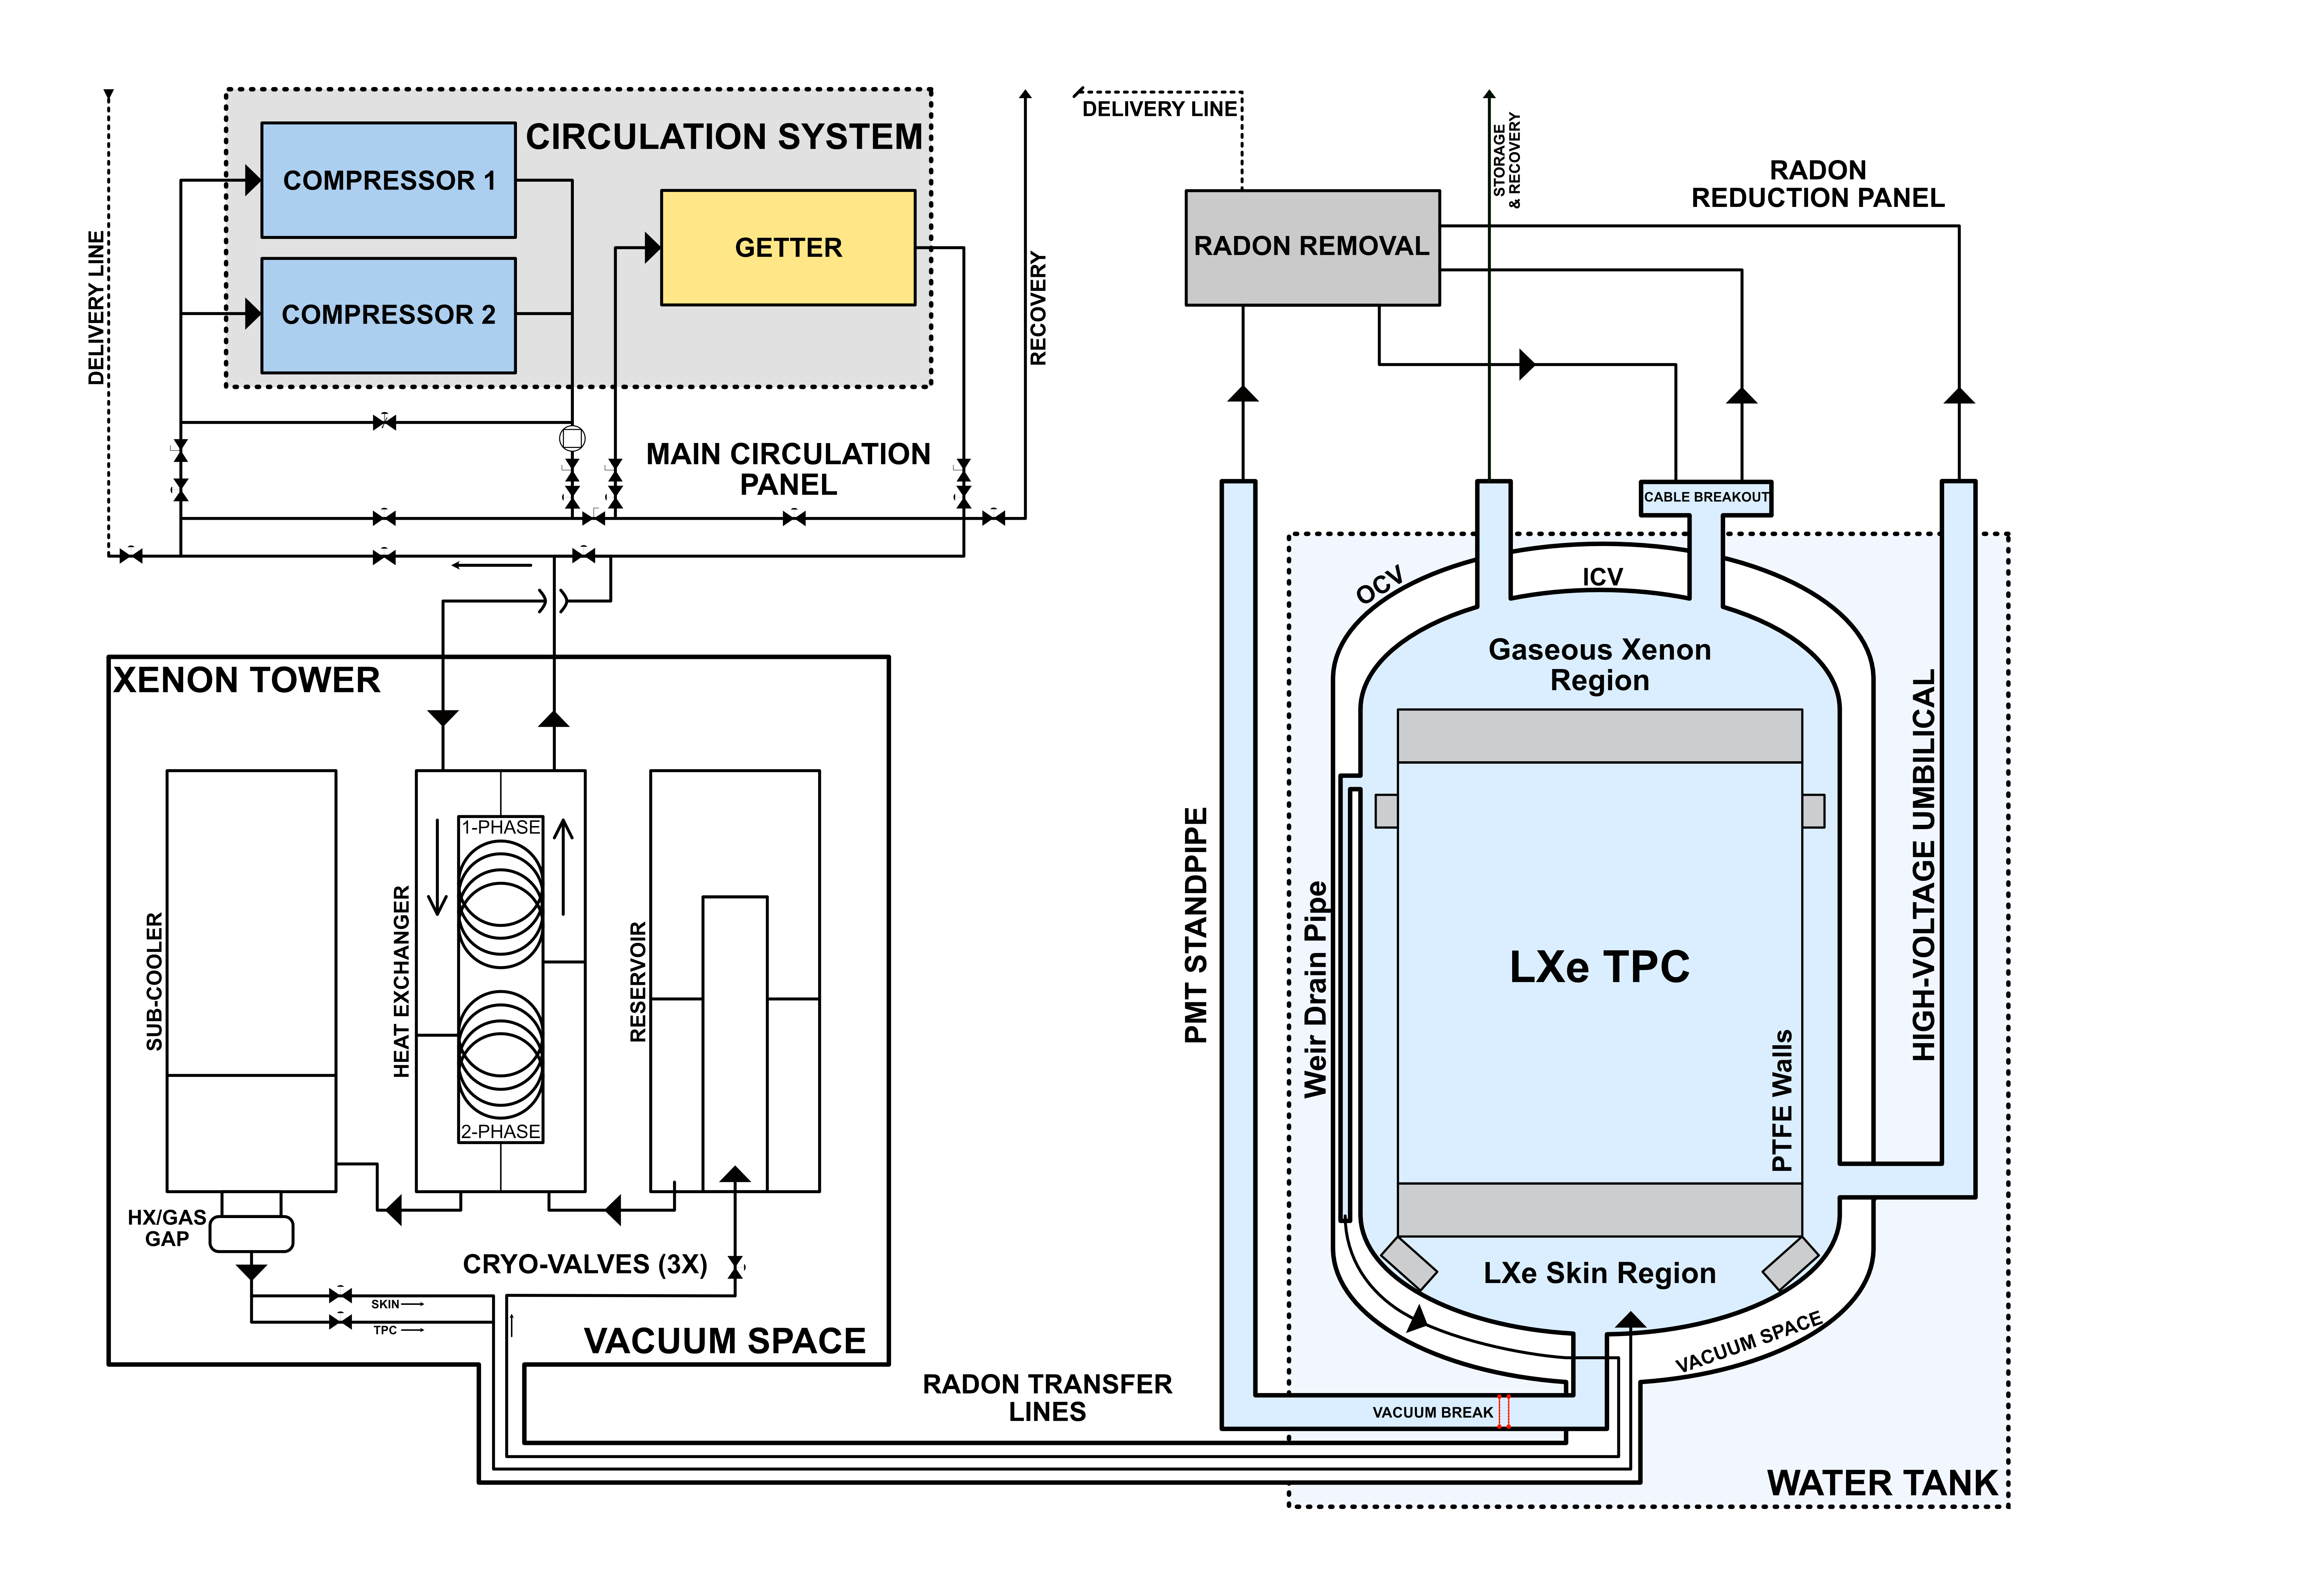
\includegraphics[scale=0.30]{Chapter_2/Figures/LZ_Xenon_Circulation.png}
    \caption[Schematics of the LZ circulation system, detailing TPC, the xenon tower and the compressor systems.]%
    {A simplified overview of the LZ circulation system. Majority of the xenon is held within the TPC, mostly in the liquid phase, with the gaseous region starting just above the weir drain opening. The LXe spills into the weir drain and through the xenon tower, which serves to heat the LXe using a two phase heat exchanger. The gaseous xenon is pumped through a hot zirconium getter, and returned to the detector after condensing. A radon removal system treats Xe gas in the cable conduits and breakout feed-throughs before sending it to the compressor inlet.}
    \label{fig:circulation_diagram}
\end{figure}
%

An overview of the cryogenic and xenon handling systems are shown in the schematic in figure \ref{fig:circulation_diagram}. The temperature inside of the ICV is maintained by a set of closed-loop thermosyphon heat pipes with nitrogen as the process fluid. In operation, the liquid inside of the TPC is drained through the weir pipes, flowing into the xenon tower, which is a cryogenic system sitting outside of the water tank. The tower consists of four vessels: the reservoir vessel, the two-phase heat exchanger (HEX), the subcooler vessel, and the subcooler HEX. The tower acts as a system to convert xenon from either a liquid-to-gas phase or a gas-to-liquid phase. The circulation is established by the use of two all-metal diaphragm gas compressors (model No. A2-5/15) from Fluitron, circulating the gas through a hot zirconium getter at a design flow rate of 500 standard liters per minute (SLPM), taking 2.4 days to purify the full 10 tonne Xe inventory in a single pass. After the removal of electronegative species and calibration sources such as tritium or \COF{}, the xenon is pumped through the cryogenic tower and back into the TPC and the skin region.


\subsection{Outer Detector}
\label{subsec:od}}


The outer detector (OD) system consists of a set of 10 segmented acrylic tanks surrounding the ICV, as highlighted in figure \ref{fig:od_tanks}. The segments are filled with a total of 17.3 tonnes of liquid scintillator. The scintillation medium consists of a linear alkylbenzene (LAB) solvent doped at 0.1\% by mass with gadolinium \cite{YEH2007329}. The primary purpose of the scintillation system is to veto neutrons and \grays{} originating from radioactive impurities in material immediately adjacent to the TPC. The OD is designed to optimise the capture and tagging of neutrons within a time window that allows the signals to be correlated with the NR in the TPC. The secondary purpose of the system is to serve as an additional detector in constructing more accurate background rates for both neutrons and \grays{}. 
%
\begin{figure}[b!]
    \centering
    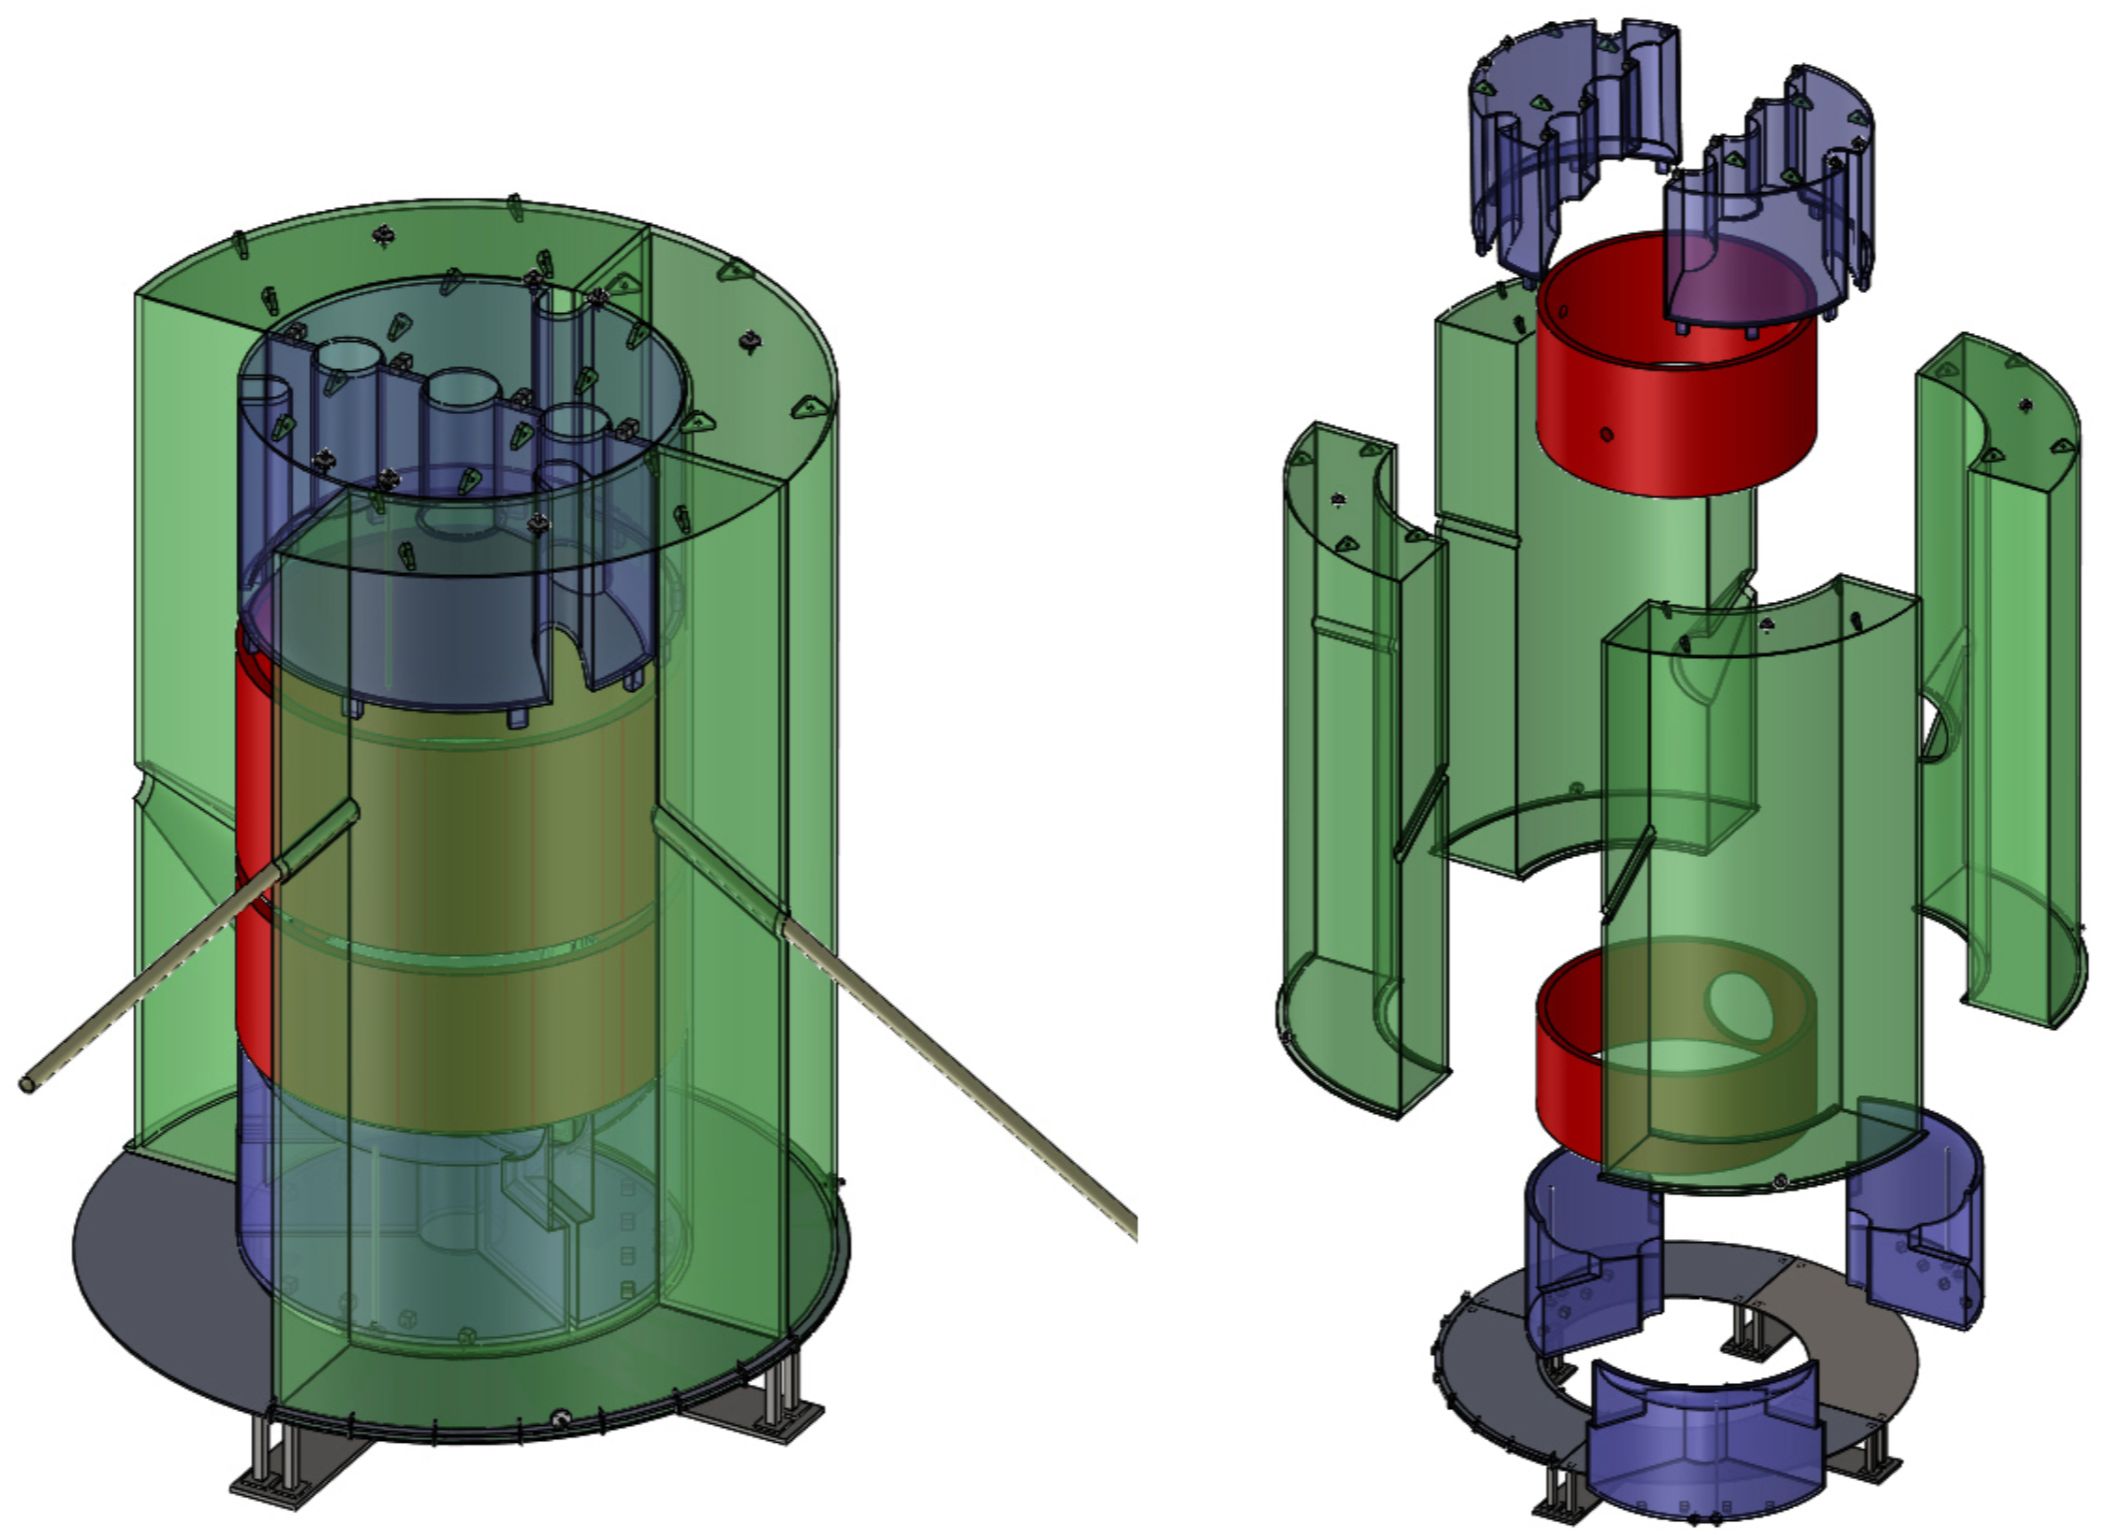
\includegraphics[scale=0.60]{Chapter_2/Figures/LZ_Outer_Detector.png}
    \caption[Schematic diagram of the liquid scintillator acrylic tanks.]%
    {Schematic diagram of the liquid scintillator acrylic tanks. The four green tanks will cover sides, while the blue will cover above and below the OD. Displacer cylinders are shown in red \cite{lz_tdr}.}
    \label{fig:od_tanks}
\end{figure}
%

Most neutrons ($\sim90\%$) are detected predominantly through a neutron capture process with the \gdoFf{} and \gdoFs{} isotopes. Upon capture, multiple \grays{} emitted, totaling 7.9 MeV (\gdoFf) or 8.5 MeV (\gdoFs). The remaining neutrons ($\sim10\%$) are captured on hydrogen, emitting a single 2.2 MeV gamma. The emitted gammas induce scintillation within the GdLS, which are collected by 120 8-inch PMTs arranged in a cylindrical array of 20 ladders that sit on support structures inside of the water tank. The light collection efficiency is further optimised by the use of Tyvek curtain that coat above, below and behind the PMT structure, and a layer surround the cryostat.


\subsection{Calibrations}
\label{subsec:calibrations}

The calibration campaign developed for LZ is a multi-purpose effort to understand accurately and precisely the response of instruments, different detection regions and the underlying xenon response for both ER and NR interactions at varying energy scales. To achieve this, LZ will utilise on internal and external calibration sources, using a range of radioactive nuclide sources. A list of these sources with key highlights are summarised and presented in table \ref{tab:calibration_sources}.

The deployment of internal calibration sources is necessary due to the self-shielding properties of LXe. To overcome this, known amounts of specific isotopes are injected into the circulation system, from which a uniform mixing with LXe in the active region can be achieved. The baseline set of internal sources include short-lived isotopes such as \KrETm{}, \XeOTOm{} and \RnTTZ{} that are stored in the form of their parent nuclide that can be handled and stored in a compact solid form. Additionally, long-lived sources such as \HT{} and \COF{} can be stored as pressurised gas with purified Xe serving as the carrier. The removal of long-lived isotopes is critical and hence their form of deployment must be in a chemical form that can be effectively removed by the getter. Both long-lived and short-lived gaseous sources require precise dose control on the injected activity, accomplished via a gas handling system dedicated to injection control.

The external sources are predominantly used to calibrate nuclear recoil response and are achieved via two distinct methods. The first of these lower sources into the vacuum region between the ICV and the OCV with a deployment system which raises and lowers the source through three conduits with a position accuracy of $\pm5 \; \MathText{mm}$. A selection of photoneutron ($\gamma, n$) sources, as listed in table \ref{tab:calibration_sources}, are planned to calibrate the nuclear recoil energy range from below 1 keV up to about 4.6 keV. This energy region is of particular interest as \BE{} solar neutrino coherent scattering falls within this window. A second method to calibrate higher energy NR response is by using a deuterium-deuterium (DD) neutron generator that produces up to $10^{8}$ neutrons per second. The setup will sit outside of the water tank delivering neutrons through the outer detector via a dedicated neutron conduits. This source has already been used by LUX to obtain a precise, in-situ calibration of the low-energy nuclear recoil response \cite{lux_dd}.

\begin{table}[h]
\centering
\caption
[Overview of the radioactive nuclide sources planned for LZ calibration, highlighting the type of interaction, energy deposition range, half-life of the isotopes and their intended purpose.]
{Overview of the radioactive nuclide sources planned for LZ calibration, highlighting the type of interaction, energy deposition range, half-life of the isotopes and their intended purpose. The partitioned sections represent different deployment techniques. 1$^{st}$: Internal gaseous sources. 2$^{nd}$: Sealed sources lowered down small-diameter conduits to cryostat side vacuum, 3$^{rd}$: \gammaN{} sources that are deployed as indicated in (2), but require dense shielding. 4$^{th}$: DD generator sources, in which neutrons travel through conduits from the generator.}
\label{tab:calibration_sources}
\vspace{1mm}
\renewcommand{\arraystretch}{1.2}
    \begin{tabularx}{1.0\linewidth}{@{\extracolsep{\fill}}lllll}
    \toprule
    
    \textbf{Isotope} & %1
    \textbf{Type} & %2
    \textbf{Energy [keV]} & %3
    \textbf{$\tau_{1/2}$} & %4
    \textbf{Purpose} & %5
    \hline
    \hline
    
    \HT{}	 & \beta{}       & 18.6 endpoint    & 12.5 y            & ER band \\ 
    \COF{}	 & \beta{}       & 156 endpoint     & 5730 y            & ER band \\ 
    \KrETm	 & \gamma{}      & 9.4, 32.1        & 1.83 h            & TPC ($x,y,z$) \\ 
    \XeOTOm	 & \gamma{}      & 164              & 11.8 d            & TPC ($x,y,z$), Xe skin \\ 
    \RnTTZ{} & \alpha{}, \beta{},  \gamma{} & various   & 10.6 h    & Xe skin \\ 
    
    \hline
    
    \NaTT{}	 & \gamma{}       & 511, 1275       & 2.61 y      & TPC and OD sync \\ 
    \MnFF{}	 & \gamma{}       & 835             & 312 d       & High-energy ER response \\ 
    \CoFS{}	 & \gamma{}       & 122             & 0.74 y      & Xe skin \\ 
    \CoSZ{}	 & \gamma{}       & 1173 , 1333     & 5.27 y      & High-energy ER response \\ 
    \BaOTT{} & \gamma{}       & 356             & 10.5 y      & ER response \\ 
    \ThTTE{} & \gamma{}       & 2615            & 1.91 y      & High-energy ER response \\ 
    \AmLi{}	 & \alphaN{}      & 1500 endpoint   & 432 y       & NR band \\ 
    \AmBe{}	 & \alphaN{}      & 11,000 endpoint & 432 y       & NR band \\ 
    \CfTFT{} & \neutron       & Watt spectrum   & 2.65 y      & NR efficiency \\ 
    
    \hline
    
    \YBe{}	    & \gammaN{}     & 152       & 107 d     & NR response \\ 
    \SbBe{}	    & \gammaN{}     & 22.5      & 60.2 d    & NR response \\ 
    \BiBeTZF{}	& \gammaN{}     & 88.5      & 15.3 d    & NR response \\ 
    \BiBeTZS{}	& \gammaN{}     & 47        & 6.24 d    & NR response \\ 
    
    \hline
    
    \DD{}	& \neutron{}        & 272 \xrightarrow{} 400        & ---     & NR light and charge yields \\ 
    \DD{}	& \neutron{}        & 2450                          & ---     & NR light and charge yields \\
    
    \bottomrule
    \end{tabularx}
\end{table}
  \chapter{Radiogenic backgrounds in LZ}
\label{chap:chap3}

The understanding of backgrounds and their origin in a low-background dark matter detector is critical for the search for dark matter. Without fully understanding and mapping all background sources, the ability to ascribe a statistical significance on any potential excess becomes ever more difficult. Moreover, this understanding is extremely important in sourcing detector material, strategising cleanliness protocols for construction, and approximating the expected background for a potential search. This chapter will discuss background sources in LZ and their origin, highlighting the techniques used for the extensive screening campaign for material selection and detector construction.  

%%------------------------------$$
%%------------------------------$$
\section{Overview}

The backgrounds as seen by the LZ detector can predominantly be characterised under two classes: electron recoils that occur when radioactive species interact with the electrons of the xenon target; and nuclear recoils, which occur when species interact with the nucleus of the xenon target. WIMPs are expected to scatter via nuclear recoils, hence any background that undergoes this type of interaction is irreducible and has the largest impact to WIMP sensitivity. Although electron recoils can be discriminated to a degree, recombination fluctuations as described in section (\ref{subsec:s1}) can lead to ER leakage into the NR band. Therefore, any and all sources that contribute towards ER and NR backgrounds are subject to extensive examination before and during detector construction.

The sources of backgrounds contributing to overall ER and NR rates can be categorised as those that are internal to the detector and those that are external. Internal backgrounds are defined to be those that are locked into the detector; originating from fixed material contaminants, surface contaminants and xenon contaminants. External backgrounds include those from laboratory and cosmogenics. This chapter will predominantly focus on fixed contaminants, surface contamination and contributions from the laboratory. Backgrounds from radon emanation---a xenon contaminant---will later be discussed in detail in section (\ref{chap:chap4}). Additional backgrounds, such as those from solar and atmospheric neutrino, or the double-beta decay of \xeOTS{} are search specific and will become more relevant in section (\ref{chap:chap5}).

To maximise sensitivity, LZ requires very low radio-contamination, both intrinsic to materials and contaminants due to exposure. The LZ radioassay program was constructed to screen and source the most radio-pure materials available. The techniques used in the screening process include various forms of gamma and mass spectroscopy; to probe the intrinsically locked radiogenic species. Furthermore, upon completion of material selection, material handling in the transportation and construction process is of great importance in reducing surface contamination. The following sections will give an introduction to the origin of these backgrounds, the techniques used to screen, and the cleanliness protocols developed to monitor and keep surfaces clean in the construction process. 

%%------------------------------$$
%%------------------------------$$
\section{Background Origins}
\label{sec:background_origins}

\subsection{Fixed Contaminants}
\label{subsec:fixed_contaminants}

Naturally occurring radioactive species are often embedded in raw materials with unknown levels of activity. The most prevalent are those of \UTTE{}, \UTTF{}, \ThTTT{} and their progeny, which eventually decay down to a stable isotope of lead via the emission of multiple \alpha{}, \beta{} and subsequent \grays{}. The \UTTE{} and \ThTTT{} chains are particularly dangerous as they often lead to electron and nuclear recoils within the WIMP energy region of interest, the latter through (\alpha, n) reactions within detector materials. 
Measuring the entirety of these chains present a challenge as they contain a number of isotopes with half-lives ranging from milliseconds to billions of years. Often it can be assumed that these chains are in secular equilibrium; a situation that arises due to the relatively long half-lifes of parent nuclei in comparison to their daughter nuclei. Hence, a measurement of the activity in one part of the chain can be used to infer the activity of the rest. 
However, \UTTE{} and \ThTTT{} chains, as shown in figure (\ref{fig:u_238_and_th_232}) are divided into \textit{early} and \textit{late} chains, representing the activity of U/Th as approximated by measurements on isotopic decays above or below the radium isotope on both chains. This distinction is particularly important for \UTTE{} as the \RaTTS{} has a half-life of 1600 years; hence a breakage in secular equilibrium due to a chemical process will take thousands of years to be restored. \UTTEe{} will refer to the \UTTE{} activity as measured above \RaTTS{}, and \UTTEl{} will represent the activity measured from \RaTTS{} and below. A similar approach is taken for \ThTTT{}, with \ThTTTe{} and \ThTTTl{} representing activities above \RaTTE{} isotope and the latter part of the chain.
%
\begin{figure}[t!]
    \begin{center}
        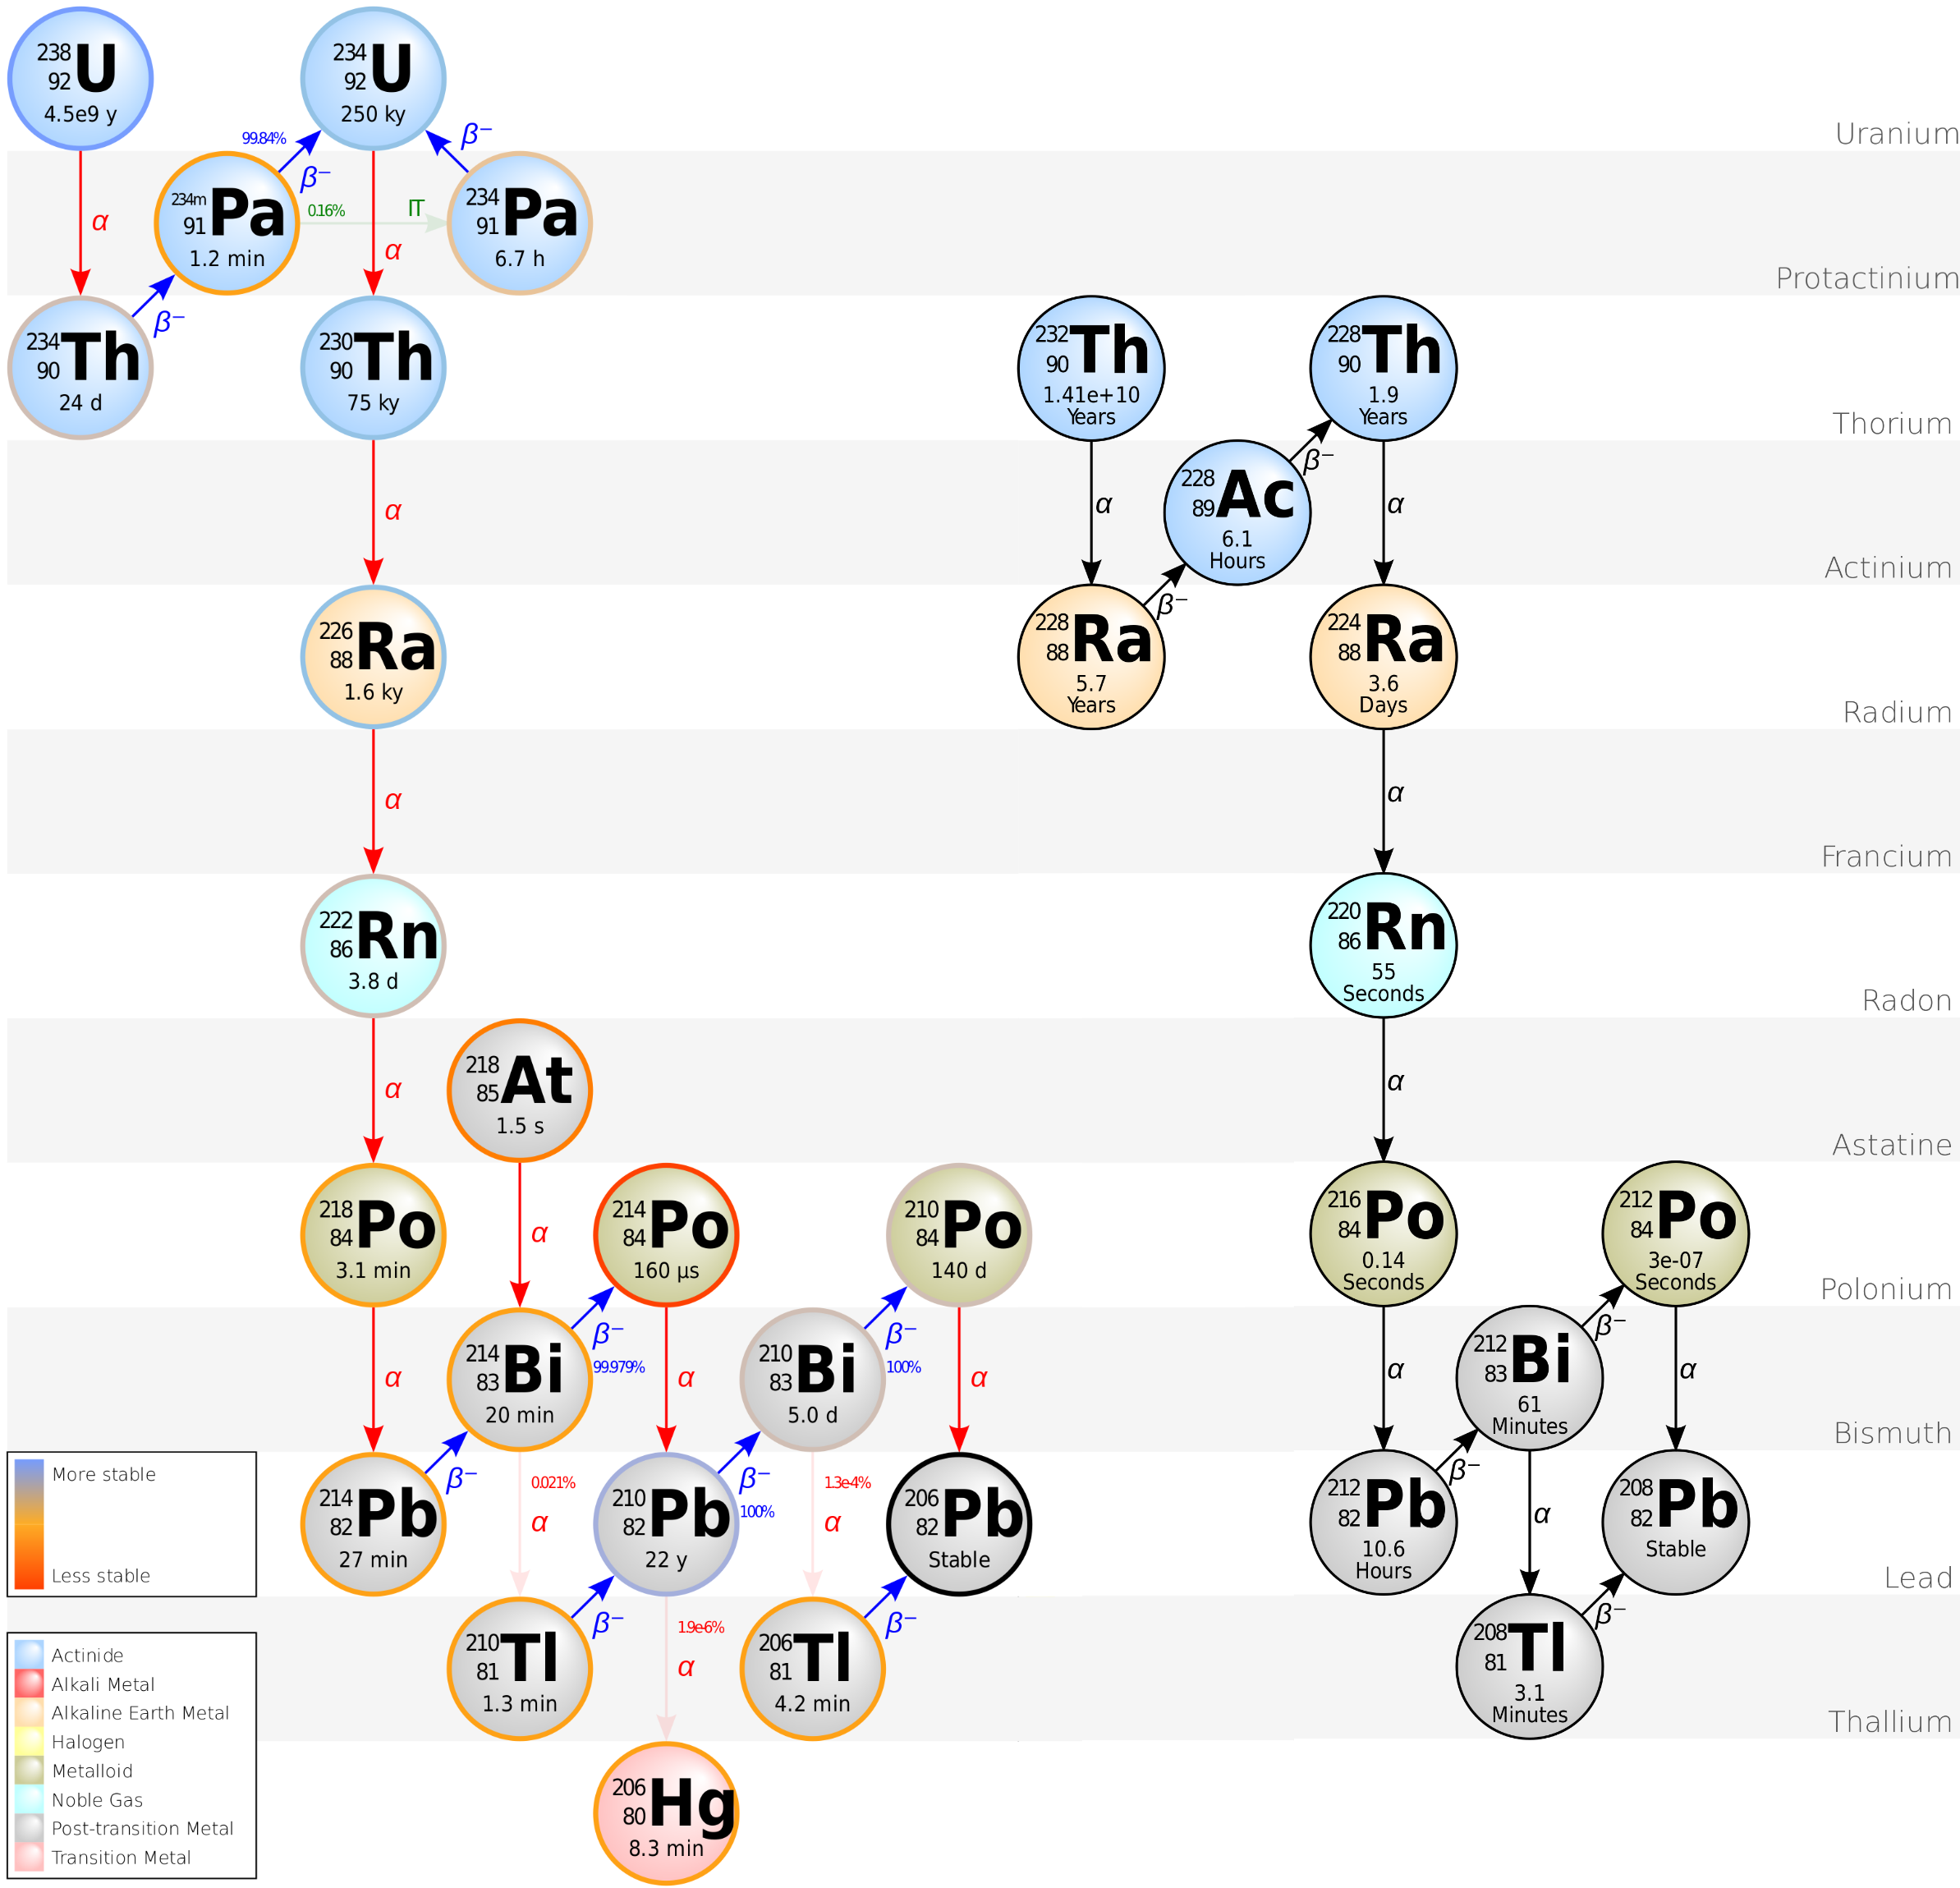
\includegraphics[scale=0.75]{Chapter_3/Figures/U_Th_Chain.png}
        \caption[Isotopes if the \UTTE{} and \ThTTT{} decay chains, detailing their half-lifes and decay types.]%
        {Isotopes of the \UTTE{} and \ThTTT{} decay chains, detailing their half-lifes and decay types. Its important to note that this is a simplified diagram and decays detailed here may occur through other mechanism.}
        \label{fig:u_238_and_th_232}
    \end{center}
\end{figure}
%


Furthermore, \gray{} emitting isotopes such as \KFZ{}, \CoSZ{} and \CsOTS{} are also present in many material and are a part of the material screening process. \KFZ{} is present within natural potassium at levels of 0.012\%, whereas \CoSZ{} can be produced via neutron activation of naturally occurring \CoFN{}, and \CsOTS{} is often formed as one of the more common fission products by the nuclear fission of \UTTF{}. While these isotopes are often identified and measured by their \gray{} emissions, they all emit \beta particles at range of energies, with the highest endpoint of 1.311 MeV from the \beta-decay of \KFZ{}. Hence, they often result in electron recoils with a wide energy spectrum.

\subsection{Surface Contaminants}
\label{subsec:surface_contaminants}

Fixed contaminants as highlighted in section (\ref{subsec:fixed_contaminants}) are naturally found in material, with their isotopic activities expected to stay constant from the point of screening, to their implementation and usage inside the detector. This however does not hold true if a chemical process was conducted between the period of screening and construction. However, there are other mechanisms at play which can change the global activity of a material through surface contamination.

Contamination of surfaces can take place whenever a detector material is exposed. Contamination can occur through multiple mechanisms: contamination due to exposure to other material, environmental dust, and isotopic plate-out. However, the specific isotope of importance is the \PbTOZ{} ($\tau_{1/2} = 22.3 \; \MathText{y}$) isotope in the \UTTE{} decay chain. Due to the relatively long half-life of \PbTOZ{}, the isotope can serve as another point of breakage in secular equilibrium. Material exposure to air with \RnTTT{} can result in the plate-out of radon daughters onto surfaces \cite{Bruemmer_2015, Stein_2018}. This process serves as a mechanism to increase the activity of \PbTOZ{} relative to the intrinsic activity driven from fixed contamination. Exposure to other materials, and more importantly environmental dust, can also yield as a mechanism to increase the activity of isotopes in the late chain. The later contaminant not only increases the activity of \PbTOZ{}, but the entire late chain, as the dust particulates will be locked into surfaces with specific concentrations of \UTTE{} and \ThTTT{}.

Plate-out and dust accumulation leads to the generation of both ER and NR backgrounds. ER backgrounds originate from the \PbTOF{} naked betas in the \RnTTT{} sub-chain, leading to a continuous ER background down to the WIMP energy window. NR backgrounds are increased due to the increase in the \alpha-rate, which in turn increases the rate of \alphaN{} processes that release neutrons into the xenon. Furthermore, \PoTOZ{} ions from the \PbTOZ{} sub-chain originating at the edge of the TPC are likely to be misreconstructed as NRs within the fiducial volume. \PoTOZ{} on material surfaces will recoil into the LXe volume producing a complicated wall background (0 to 103 keV in energy). The impact of the latter depends critically on the performance of position reconstruction and drives the 4 cm radial fiducial volume cut. LZ has instituted a target for plate-out of \PbTOZ{} and \PoTOZ{} of less than 0.5 mBq/m$^{2}$ on the TPC walls and below 10 mBq/m$^{2}$ everywhere else. LZ has also instituted a requirement limiting generic dust contamination to less than 500 ng/cm$^{2}$ on all wetted surfaces in the detector and xenon circulation system. 

\subsection{Other Source Origins}
\label{subsec:other_bkkg_sources}

\subsubsection{Xenon Contaminants}

Natural xenon includes trace levels of \KrEF{} and \ArTN{}, both of which disperse throughout the liquid and are beta emitters that lead to ER events in the ROI. To reduce the levels of \KrEF{} within the LZ xenon, a purification campaign using chromatography to remove krypton from xenon has been implemented \cite{lz_tdr}. The system has been shown to reduce \KrNAT{}/Xe concentration to 0.075 ppt g/g. A further reduction in the levels of argon has also been observed, with an expected concentration of \ArNAT{}/Xe below 0.45 ppb g/g.

Cosmogenic activation of xenon isotopes can also lead to an overall increase in  background rates. The activation rate depends heavily on the depth at which the xenon is stored, as more activation is expected at sea level due to the cosmic ray flux. The equilibrium decay rate of \XeOTSeven{} ($\tau_{1/2} = 36.4 \; \MathText{d}$), a cosmogenic background, was measured by LUX to be ($2.7 \pm 0.5$) mBq/kg after xenon was exposed to cosmic rays on the Earth’s surface \cite{radiogenic_muon_lux}. Further contaminants include \XeOTNm{} ($\tau_{1/2} = 8.9 \; \MathText{d}$), \XeOTOm{} ($\tau_{1/2} = 11.9 \; \MathText{d}$) and \XeOTT{} ($\tau_{1/2} = 5.3 \; \MathText{d}$). Due to their short half-lives, a short cooling period ($\sim$8-months) of the xenon underground before data taking reduces this background significantly. 


\subsubsection{Cosmogenic Activation of Materials}

Cosmogenic activation can also impact detector material, especially during the sourcing and construction phase, which predominantly takes place in the Earth's surface. At SURF, the location of LZ operations, the muon flux was measured at ($1.149\pm0.017$)$\times10^{-2}$ s$^{-1}$cm$^{-2}$sr$^{-1}$ \cite{surf_muon_flux}. The primary concern from cosmogenic material activation is the production of \ScFS{} ($\tau_{1/2} = 83.8 \; \MathText{d}$). Generated by either muon capture or an \alphaN{} reaction in titanium, \ScFS{} decays via a \beta{}-decay with an endpoint energy 0.357 MeV, with a subsequent emission of two \grays{} of energies 889 keV and 1,121 keV. The production and the decay modes are given as,
%
\begin{equation} \label{eq:cosmogenic_activation}
    ^{46}_{22}\MathText{Ti} + \mu{}^{-} \; &\rightarrow \; ^{46}_{21}\MathText{Sc} + n + \nu{}_{\mu{}} \\
    ^{46}_{22}\MathText{Ti} + n \; &\rightarrow \; ^{46}_{21}\MathText{Sc} + p \\
    ^{46}_{21}\MathText{Sc} \; &\rightarrow \; ^{46}_{22}\MathText{Ti} + e^{-} + \nu{}_{e}.
\end{equation} 
%


\subsubsection{Muon-Induced Neutron Background}

Despite 4850-foot (4300 m w.e.) of Earth sitting above the Davis laboratory at SURF, although suppressed in comparison to surface level, a muon flux of ($4.4\pm0.1$)$\times10^{-9}$ s$^{-1}$cm$^{-2}$ is still present \cite{muon_davis}. In detector material and xenon, this flux generally generates internal backgrounds as discussed above. In the laboratory, neutrons from muon-induced electromagnetic and hadronic cascades within the cavern walls can generate background events. The neutron flux from the laboratory walls have been estimated using simulations of muon transport through rock around the laboratory and detector geometry. Attenuation through the water tank and the outer detector scintillators reduces the integrated neutron flux by more than 6 orders of magnitude \cite{TOMASELLO201070} resulting in a negligible contribution to backgrounds in LZ. Its important to note that this mode of background generation may become more significant, if experiments were running closer to the surface.


%%------------------------------$$
%%------------------------------$$
\section{Fixed Contaminant Screening Techniques}
\label{sec:fixed_contaminant_screening}

Approximating and modelling the expected backgrounds originating from fixed contaminants, as covered in detail in section \ref{subsec:fixed_contaminants} has been a high priority for the LZ experiment; initially in selecting radio-pure material for the LZ detector, but also to inform the background model through a combination of screening results, attained from many different screening techniques and detector. The ability to radioassay materials to ever increasing levels of sensitivity, within a short time period is of great importance as the next-generation low-background experiments are probing evermore sensitive parameter spaces. 

In screening for fixed contaminants, the LZ screening campaign has made use of various techniques, including but not limited to an array of high-purity germanium (HPGe) detectors and inductively-coupled plasma mass spectrometry (ICP-MS). The following sections will summarise these techniques within the scope of LZ; focusing on the Boulby underground germanium suite (BUGS) \cite{bugs_boulby} and the ICP-MS facility at University College London (UCL) \cite{icpms_ucl}. 


\subsection{High-Purity Germanium Screening}
\label{subsec:HPGe}

Gamma ray spectroscopy is a technique that uses the principles of interaction of gamma radiation with matter to interpret and measure the activities of specific radio-isotopic impurities within material. The incoming \gray{} photons often deposit their energy by transferring up to all of its energy to the absorbing material through the mechanisms of photoelectric absorption, Compton scattering and pair production. The resultant secondary particles, often electrons, will then induce excitation and ionisation within the material to elude to the nature of the incoming photon. These are various different absorption material, detector design and types of operation to probe a wide range of photon energies but, the primary focus in this section will be germanium semiconductor diodes detectors. Details into the wider theoretical and practical use cases of \gray{} spectroscopy are provided in \cite{gilmore2011practical}.

\subsubsection{Germanium Detectors}

Germanium detectors are a class of semiconductor detectors that are widely used in \gray{} spectroscopy. Their relatively high atomic number, Z; suitability in allowing for large crystalline growth with impurity levels of $10^{10} \; \MathText{atoms/cm}^3$ or lower; and the energy resolution achieved due to their very low bandgap ($E_{g} \approx 1 \; \MathText{eV}$), make them a prime candidate for keV--MeV \gray{} detection. 

The periodic lattice formation in germanium crystals lead to distinct band formation for electrons that exist within the solid. The \textit{valence band} corresponds to outer-shell electrons that form covalent bonds within the crystal; the \textit{conduction band}, sitting at a higher energy level, represents the band in which electrons are free to migrate through the crystal. The excitation of an electron from the valence band to the conduction band often takes place due to thermal energy. In doing so, it places an electron into the conduction band that is free to drift, but also creates what's known as a vacancy (hole) in the otherwise full valence band---the combination of these is called an \textit{electron-hole} pair. The electron in the conduction band and the subsequent hole can both be drifted if an electric field is applied to the crystal; though in opposite directions, as the hole represents a net positive charge. The resultant drifted charge is then collected using electrodes

The electrical properties of commercial crystals is often dominated by the small residual impurities that remain within such crystals. The nature of these impurities determine the type of semiconductor present; often labeled as an \textit{n}- or \textit{p}-type. In \textit{n}-type crystals, the impurities occupy sites within the lattice and have en extra valence electron in their outer-shell. Often referred to as \textit{donor impurities}, they readily contribute electrons to the conduction band. In such material, the majority charge carriers are electrons. In \textit{p}-type, the impurities often have one less valence electron relative to the crystal, effectively increasing the number of holes within the entire crystal. Referred to as \textit{acceptor impurities}, these sites capture electrons excited to the conduction band; hence the majority charge carrier in such material are the excess holes that are formed within the material. Materials can often be doped with specific impurities to determine the nature of the crystal.


\subsubsection{Boulby Underground Germanium Suite (BUGS)}

The Boulby Underground Germanium Suite (BUGS) hosts seven gamma spectroscopy detectors \SI{1.1}{\km} underground at the Boulby Underground Laboratory in a class 1000 cleanroom. Since 2013, majority of the gamma spectroscopy screening efforts in LZ were conducted by the Chaloner (Mirion BE5030 broad-energy ultra-low background (ULB) HPGe detector), Lunehead (Mirion ULB SAGe well-detector), and Lumpsey (Ortec p-type detector) detectors. Prior to LZ, these detectors were extensively used for the ZEPLIN--II and ZEPLIN--III experiments \cite{Alner:2007ja, Araujo:2011as}. In addition to these detectors, BUGS has installed additional Mirion ``specialty ultra-low background'' (S-ULB) detectors which have been used to screen later LZ samples since 2017. These comprise two p-type detectors, Belmont and Merrybent, with relative efficiencies of \SI{160}{\percent} and \SI{110}{\percent}, respectively, and Roseberry, a BE6530 BEGe type detector.

The shielding of such detectors is detrimental to their operational output. The idea behind these detectors is to limit the \grays{} hitting the crystals strictly to those originating from the sample of interest. \grays{} originating either from detector material or external sources are considered to be background. The BUGS detectors are housed in custom shields designed and built by Lead Shield Engineering Ltd. The shields comprise 9 {\cm} thickness of lead and 9 \cm thickness of copper with interlocking retractable roofs to simplify sample loading. The lead used in these shields has mostly been recycled from lead used to shield previous low-background experiments hosted at the Boulby Underground Laboratory. The characterizations and sensitivities of these detectors are discussed in \cite{bugs_boulby}.

\grays{} originating from the \RnTTT{} sub-chain in the air can also contribute towards the background rate. To reduce such background, the shields used for all detectors are purged using nitrogen from a Wirac NG6 gas generator. The Boulby Underground Laboratory benefits from a low baseline radon level (averaging \SI{\sim 2.5}{\becquerel\per\m\cubed}). To remove residual radon in the nitrogen purge gas, charcoal traps containing approximately \SI{6}{\kilogram} of Carboact activated charcoal are deployed in a Labcold ULTF416 -80C chest freezer. This radon reduction system is based on the design of a radon emanation detector developed at the Centre de Physique des Particules de Marseille (CPPM)~\cite{Noel:2015nla}. 


\subsubsection{Other \gray{} Screening Facilities for LZ}

Other than BUGS, LZ employs various other \gray{} screening facilities, including the Black Hills Underground Campus (BHUC) \cite{Mount:2017iam}, located at the 4850-foot level of SURF which hosts a class 2000 clean-room containing seven low and ultra-low background HPGe detectors; Lawrence Berkeley National Laboratory (LBNL) \cite{Smith:2015aoa}, which operates two HPGe detectors devoted to assay; and University of Alabama operating two above-ground Canberra p-type low-background HPGe detectors \cite{Tsang:2019apx}.

The LZ radioassay program uses a total of 12 detectors from the facilities mentioned above. A more detailed description of these facilities and their housed detectors can be found in the ``LUX-ZEPLIN (LZ) radioactivity and cleanliness control programs'' paper \cite{lz_screening}. A summary of the 12 detector used by LZ, detailing the type of detector and some key characteristics can be found in table \ref{tab:GeDetInf}.

\begin{table}[h]
\centering
\caption
[Key characteristics of the 12 detectors used in the LZ HPGe screening campaign.]
{Key characteristics of the 12 detectors used in the LZ HPGe screening campaign. Crystal mass and volume is included to give an idea of the relative sizes of the crystal. In addition the relative efficiency is given for the p-type detectors and the area of the front face is given for the BEGe detectors \cite{lz_screening}. For historical reasons, the relative detection efficiency of coaxial
germanium detectors is defined at 1.33 MeV relative to that of a standard 3" diameter by 3" long NaI(Tl) scintillators.}
    \label{tab:GeDetInf}
    \vspace{1mm}

    \renewcommand{\arraystretch}{1.2}
    \begin{tabularx}{1.0\linewidth}{@{\extracolsep{\fill}}lllcccc}
    \toprule
    
    \multirow{3}{*}{\textbf{Location}} & %0
    \multirow{3}{*}{\textbf{Detector}} & %0
    \multirow{3}{*}{\textbf{Type}} & %1
    \multirow{2}{*}{\textbf{Volume}} & %2
    \multirow{2}{*}{\textbf{Mass}} & %3
    \textbf{Relative} & %4
    \textbf{Face} %5
    \\
    &
    & %0
    & %1
    \multirow{2}{*}{\textbf{[cm$^{3}$]}} & %2
    \multirow{2}{*}{\textbf{[kg]}} & %3
    \textbf{Efficiency} & %4
    \textbf{Area} %5
    \\
    &
    & %0
    & %1
    & %2
    & %3
    \textbf{(\%)} & %4
    \textbf{[cm$^{2}$]} %5
    \\
    \hline
    \hline

    \multirow{6}{*}{BUGS} & Belmont & p-type & 600 & 3.2 & 1.92 & - \\
    & Merrybent & p-type & 375 & 2.0 & 1.87 & - \\
    & Lunehead & p-type & 375 & 2.0 & 1.86 & - \\
    & Roseberry & BEGe & 170 & 0.9 & - & 181.1 \\
    & Chaloner & BEGe & 150 & 0.8 & - & 1053.0 \\
    & Lumpsey & SAGe well & 263 & 1.4 & - & - \\
    \hline
    LBNL & \textsc{Merlin} & n-type & 430 & 2.2 &3.59 & - \\
    \hline
    \multirow{4}{*}{BHUC}& \textsc{Maeve} & p-type & 375 & 2.0 &3.19 & - \\
    & \textsc{Morgan} & p-type & 375 & 2.0 & 2.68 & - \\
    & \textsc{Mordred} & n-type & 253 & 1.3 &2.44 & - \\
    & SOLO & p-type & 113 & 0.6 & 5.52 & - \\
    \hline
    \multirow{2}{*}{Alabama} & Ge-II  & p-type & 260 & 1.4 & 3.6  & - \\
    & Ge-III & p-type & 406 & 2.2 & 2.71 & - \\
    
    \bottomrule
    \end{tabularx}
\end{table}


\subsubsection{HPGe Cross-Calibration}

\begin{table}[t!]
\centering
\vspace{-5mm}
\caption{Results from the HPGe cross-calibration performed using a sample of Rhyolite. For the \utTeE{} and \utTeL{} columns, the contamination reported is that of the progenitor isotope \utTe{} assuming secular equilibrium and for the \thtTtE{} and \thtTtL{} columns, the contamination reported is that of \thtTt{} assuming secular equilibrium.}
    \label{tab:GeCrossCal}
    \renewcommand{\arraystretch}{1.1}
    \begin{tabular}{lccccc}
    
    \textbf{Detector} & %0
    \textbf{\utTeE{} (ppm)}  & %1
    \textbf{\utTeL{} (ppm)} &  %2
    \textbf{\thtTtE{} (ppm)} &  %3
    \textbf{\thtTtL{} (ppm)}  & %4
    \textbf{K ($\%$)}   \\  %5
    
    \hline
    \hline
    
    Reference & 8.87(4) & 8.5(1) & 12.1(1) & 12.1(1) & 2.82(1) \\
    
    \hline
   
    \textsc{Merlin} & 8.92(9) & - & 12.4(1) & 12.4(1) & 2.81(3) \\
    \textsc{Maeve} & 8.6(1) & 8.6(1) & 11.9(1) & 11.9(1) & 2.74(3) \\
    \textsc{Mordred} & 7.92(5) & 10.2(1) & 11.3(2) & 11.3(1) & 2.66(6) \\
    SOLO & 6.16(1) & - & 12.5(7) & 9.94(1) & 2.91(1) \\
    Chaloner & 8.73(5) & 7.9(2) & 11.1(1) & 11.1(1) & 2.81(1) \\
    Lunehead & 8.5(1) & - & 11.8(1) & 11.8(1) & 2.85(1) \\
    Ge-II & 9.6(13) & 11.4(15) & 12(16) & 12.2(17) & 3.4(4) \\
    Ge-III & 9.2(9) & 10.3(10) & 12.1(12) & 12.8(13) & 3.3(3) \\
   
    \hline
   
    Average & 7.61(3) & 9.2(2) & 11.9(1) & 10.54(0.5) & 2.84(2) \\
    Std. Dev. & 0.98 & 1.26 & 0.46 & 0.84 & 0.25 \\
    
    \bottomrule
\end{tabular}
\end{table}

The screened samples in LZ were distributed amongst the 12 detectors detailed in table \ref{tab:GeDetInf}, all with different backgrounds, shielding arrangements and operational history. To evaluate the systematic uncertainties and be able to correlate results from one detector to that of another, a sample of Rhyolite with well-characterized uranium, thorium and potassium content was used for cross-calibration. The material has been used by LBNL for over 30 years, with a well established uniformity uniformity across the sample.

An S5 Marinelli beaker of this mineral was prepared and sealed, with the content and its activity unknown to the collaboration. The comparison of results from different detectors uncovered some issues with several analyses, mostly due to problems with the Monte Carlo simulations of the detectors. These issues were identified and corrected without knowledge of the true calibration source material. The results were again compared across all the detectors. It is important to note at this point that when a concentration is reported, in parts per value ($e.g.$ ppm, ppb, ppt) it is no longer pertinent to refer to late chain or early chain values as the concentration defines the concentration of the progenitor isotope (\UTTE{ }, \UTTF{}{}, \ThTTT{}) assuming secular equilibrium~\cite{malling:2013jya}. Table \ref{tab:GeCrossCal} lists reference values for each isotope; compares results from each detector; and gives their combined average and standard deviation. The cross-calibration effort confirmed that the modeling of detector geometries and efficiencies were correctly handled and provides a reasonable estimate on the systematic variation among the assays of \SI{\sim 10}{\percent} thus giving the collaboration confidence that each individual facility is able to produce consistent and accurate assay results.


\subsection{Inductively-Coupled Plasma Mass Spectrometry}
\label{subsec:ICPMS}

Inductively-Coupled Plasma Mass Spectrometry (ICP-MS) allows very precise direct measurement of the elemental abundances of uranium and thorium in small samples. The assays can be very quick, taking hours to days depending on requisite sensitivity down to sub-ppt (\si{\gram} of U/Th per \si{\gram} of material) levels and depending on related sample preparation protocols. ICP-MS has been used extensively in LZ to quickly measure \utTe{} and \thtTt{} in small samples to either reject or clear materials for use, or to pre-screen materials prior to  assay with gamma spectroscopy which can determine the complete activity through the \utTe{} and \thtTt{} decay chains. In addition to constraining systematic uncertainty and directly determining activity at the top of the \utTe{} and \thtTt{} chains, ICP-MS has been used in LZ as part of our QC and QA program to ensure radioactivity and cleanliness compliance through component manufacture and delivery. The speed of ICP-MS allowed rapid analysis of test pieces provided by manufacturers at specified points in the production processes to detect potential issues and to ensure radioactivity and cleanliness compliance. 

The majority of ICP-MS assays for LZ were performed using a dedicated mass spectrometry laboratory at UCL, housed in a class 1000 cleanroom facility and operating an Agilent 7900 spectrometer installed in 2015 exclusively for LZ~\cite{icpms_ucl}. Sample preparation and analysis procedures have been developed for materials with U/Th concentrations in the ppt to 1 ppb range: Samples are microwave-digested in pre-cleaned modified-PTFE (TFM) vessels using ultra-high purity acids. They are then diluted, without further chemical treatment, into disposable 50 \milli{}\litre{} polypropylene (PP) vessels ready for ICP-MS analysis. Fractional recoveries of \thtTz{} and \utTT{} spikes added prior to digestion are used to correct for \thtTt{} and \utTe{} signal loss from a range of sources. In particular, this enables accurate analysis of samples with high total dissolved solids (TDS) where the instrument response degrades throughout the run. A full assay including digestion, ICP-MS measurement and analysis can be completed in a single day. The UCL facility was upgraded in 2019 with an Agilent 8900 ICP-MS. 

In addition to the system at UCL, some material samples were assayed using facilities at the University of Alabama, the  Centre for Underground Physics in Korea, and the Black Hills State University.  At the University of Alabama, the LZ group set up a sample preparation laboratory in a Class 500 cleanroom equipped with a cryogenic mill, microwave digestion system, and digestion bomb.  Further processing of samples, including spiking and resin-based extraction of U/Th isotopes was carried out in a separate cleanroom.  The samples were then given to the Department of Geological Sciences which processed the samples using a Perkin-Elmer SCIEX-ELAN 6000 system.  At Korea and Black Hills State, samples were measured using Agilent 7900 spectrometer, as was used at UCL.


%%------------------------------$$
%%------------------------------$$
\section{LZ Cleanliness Protocols \& Surface Contamination}
\label{sec:cleanliness}

Surface contamination through dust and radon daughter plate-out can lead to ER and NR generation as detailed in section \ref{subsec:surface_contaminants}. This class of contamination can take place from the second a material is manufactured up until its mounted onto the detector and protected from exposure. This section will entail dust deposition and plate-out on LZ material, focusing on the protocols used in mitigating against such contamination; techniques used in handling, modelling and estimating exposure rates on critical surfaces of the detector.


\subsection{LZ Cleanliness Protocols}
\label{secsec:cleanliness}

Often, manufacturing of detector components are sourced out to  experienced companies tailored for specialty instrumentation, such as Hamamatsu for PMTs, Loterios for the LZ cryostats and Axon for cables. And in other cases, specific instrumentation was designed and built by some of the universities involved in the project. Despite efforts in monitoring these environments for dust and radon plate-out, levels of contaminants in such environments are well above the baseline contamination requirements of the LZ project. To tackle this issue, most of the detector components after manufacturing were sent to a certified precision cleaning company, AstroPak Inc. The cleaning process involves chemical passivation or electropolishing---both of which are intended to etch surface layers of the material, removing any dust or plate-out isotopes on the surface. After these procedures, the material are sealed with radon-proof bags, either aluminised Myler or Nylon bags with reduction factors of ${2500 \pm 1042}$ and ${130 \pm 3}$, respectively \cite{Meng:2019ker}, and purged under nitrogen gas. The components are then stored safely up until their use-case in the construction process. 

Majority of LZ assembly and construction took place in the surface assembly laboratory (SAL), in SURF. The laboratory was engineered as an ISO 6 class cleanroom with an average particulate count of $\leq 10$ per cubic foot. The air filtration system was fitted with large activated charcoal columns to scrub the radon within the cleanroom to reduce the averaging activity of ambient radon level  $\leq 0.5 \; \MathText{Bq/m}^{3}$. The radon reduced cleanroom (RCR) in particular was designed with a high recirculation rate of 240.7 m$^3$/min in order to sweep out most of the radon daughters---in particularly \PoTOE---before plate-out can occur. The cleanroom was under constant dust and radon monitoring. 

Upon their use-case, the material components were taken into the RCR with their outermost seals removed, inspected for dust by ultra-violate (UV) light and fully un-sealed under de-ionising fans that served to reduce any static buildup, which was shown to be effective in reducing dust accumulation on surfaces. Majority of the critical assembly was then completed under these de-ionising fans. In situations which required further cleaning, non-shedding mini-filament (Abgenics Essence Gold) wipes saturated with \SI{99}{\percent} pure IPA was used as cleaning agents. 

Moreover, cleanroom garbs worn by personnel working on the assembly were changed after every work shift and wiped off with a lint roller multiple times during work to remove particulates that could deposit onto detector surfaces. Small detector components were sealed in double nylon bags which prevented plate-out since the components were then no longer in contact with the radon-laden air. Larger components like the cryostat vessels or PMT arrays had bespoke airtight enclosures, enabling additional filtered air and N$_{2}$ purges while in storage within the cleanroom to further mitigation against radon plate-out.


\subsection{Surface Dust}
\label{secsec:surface_dust}

The predominant source of dust that components are exposed to are as a result of outdoor air flowing into the SAL and that carried in from personnel, equipment and material. Dust monitors (Met One GT-526S particle counters) fitted in different locations of the cleanroom indicate increased levels which correlates to activity within the cleanroom. While regular cleaning of the cleanroom and the air filtration system removes most of the dust, some of which still deposits on surfaces, including some of the most critical regions of the detector, i.e. PMTs and TPC walls. To approximate deposition levels on surfaces and locked in dust amounts, two techniques have been utilised in measuring and modelling surface dust; the use of witness plates and tape-lifts. 


\subsubsection{Witness Coupons}

Witness coupons made of PTFE and glass; cleaned with isopropyl alcohol (IPA) soaked non-shedding wipes are placed in multiple locations within the RCR, serving as controlled surfaces for dust collection. Fresh coupons are often used for specific phases of the construction with the assumption that the coupons would accumulate dust at a similar rate to that of the detector surfaces exposed during that phase of construction. The PTFE and glass coupons are then screened under fluorescence and optical microscopy, respectively, and processed via an ImageJ software \cite{DBLP:journals/corr/RuedenSHDWE17} to reveal smaller particulates to determine the size distributions and their relative contributions to the dust density accumulated on the coupons' surfaces. Once the dust particulates size distribution is determined, as shown in figure (\ref{fig:dust_particle}), the dust density accumulated on the coupon (in \si{\nano\g\per\cm\squared}) is calculated by dividing the accumulated mass (assuming particulates are spherical in shape with density of 1${g/cc}$) by the surface area of the coupons. Blank rates from unexposed coupons prepared in the same manner are taken into account in the analyses by background subtraction. The results from witness plates are a good measure on average dust levels during operation but are not precise enough to estimate the actual dust accumulation on surfaces.
%
\begin{figure}[hbt!]
    \centering
    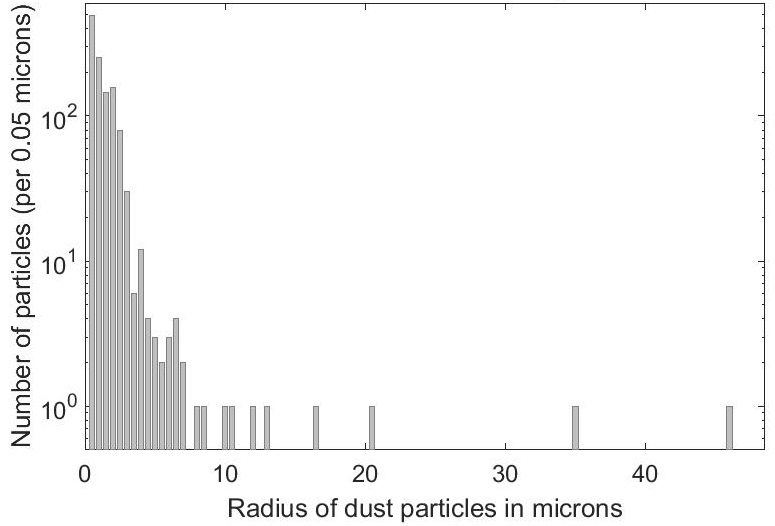
\includegraphics[scale=0.46]{Chapter_3/Figures/ParticlesByRadiusLogScale.jpg}
    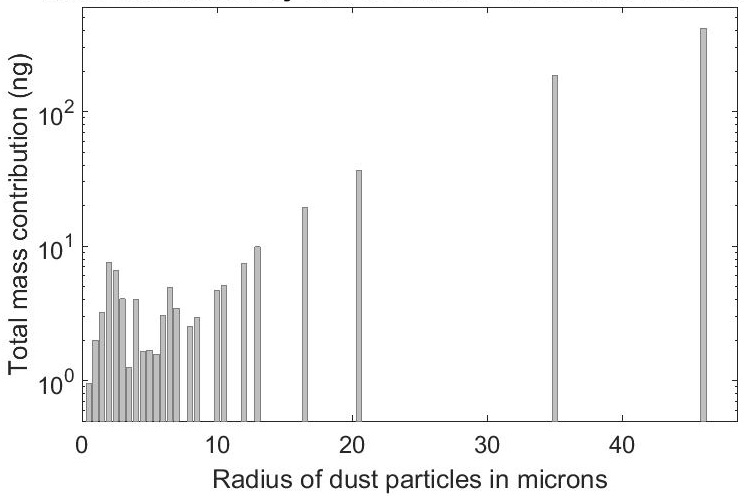
\includegraphics[scale=0.49]{Chapter_3/Figures/MassContributionLogScale.jpg}
    \caption[Dust particulate size and mass distribution from fluorescent image analysis of sample witness plates.]
    {Dust particulate size distribution (left) and mass distribution (right) from fluorescent image analysis of a witness plate. Majority of the mass on the coupon is from a small number of larger particles. Particulates of size $>50 \; \micro{}m$ are rarely recorded.}
    \label{fig:dust_particle}
\end{figure}
%


\subsubsection{Tape-lifts}

In order to fully assess the dust levels on surfaces post-construction, surfaces of detector material were sampled with acetate or carbon tapes. The tapes were applied onto surfaces to remove the accumulated dust and assayed using the same fluorescence microscopy technique utilized for the witness coupons. The choice of tape material depends on the surface roughness of the component; acetate tape works better on smooth surfaces, like PTFE, while, for rougher surfaces like titanium, carbon tapes were found to perform better. However, tape-lifts cannot be taken on particularly sensitive parts of the detector, and therefore, they do not negate the need for coupons, but rather complement them. Both tape-lifts and coupons are necessary for a full history of the dust deposition on every component during the assembly process. 


\subsection{Radon Plate-out}
\label{secsec:radon_plateout}

The presence of primordial \UTTE{} and the effect of radon emanation from the environment can vary radon levels in air from 5--15 Bq/m$^3$ and to much higher levels in indoor environments. Once in air, the consequent \alpha-decay of \RnTTT{} and daughters can lodge into material surfaces due to the kinetic energy carried as a result of the decay. As described in section (\ref{sec:cleanliness}), LZ limits the plate-out rate by assembling most of the background-prone instrumentation from plate-out in the RCR, with a continuous filtration system constantly circulating to reduce the concentrations of \RnTTT{} and daughters in the air. Absolute plate-out prevention is however not possible, and the remaining \PoTOE{} that plates out is problematic due to the long-lived \PbTOZ{} daughter which will decay over time in the detector. Therefore, the estimation of plate-out rates during assembly is crucial for operational control and background modelling.

Plate-out rates onto material are estimated using the Jacobi model \cite{jacobi1972activity, knutson1988modeling}, describing particle deposition on surfaces from a balance of in- and out-flux of concentration in a maximally mixed air model. The model assumes that all surfaces within a given enclosure have equivalent plate-out rates per area, which is a function of air circulation rate, Rn concentration, volume, and surface area within the enclosed space the material surfaces reside. The plate-out rate is given as Becquerel per unit area and time of \PbTOZ{}, where
%
\begin{equation}
    R_p=C_{Rn}\lambda_{Pb_{210}}\frac{\Lambda_d}{(\Lambda_d +\Lambda_v)}\frac{V}{A}.
    \label{eq:jacobi_eq}
\end{equation}
%
The \RnTTT{} concentration as obtained by radon monitors within the RCR (Durridge RAD7) is given by ${C_{Rn}}$ and ${\lambda_{Pb_{210}}}$ is the decay rate of \PbTOZ{}. ${{\Lambda_d =v\frac{A}{V}}}$ is the deposition rate that depends on the diffusion velocity $v$ of radon daughters measured to be between 5--15 m/h \cite{knutson1988modeling} and ${{\Lambda_v = \frac{R}{V}}}$ is the air ventilation rate obtained by dividing the recirculation rate $R$ by the volume $V$ of the cleanroom, and $A$ is the surface area of the RCR at SAL where most of the assembly work has been performed. The ratio ${\frac{\Lambda_d}{(\Lambda_d +\Lambda_v)}}$ corresponds to the probability that a radon daughter will plate-out before removal through ventilation and is calculated to be 0.17.

In estimating a plate-out rate, the Jacobi model does not differentiate between types of material. This assumption is shown to be incorrect for material with highly negative triboelectric charging---a type of contact electrification on which certain materials become electrically charged---such as PTFE \cite{zou:2019tde}. Measurements on PTFE indicate a factor of 50--100 times higher plate-out rate than for neutral metallic materials \cite{Morrison:2017xul}. PTFE surfaces within LZ therefore have a multiplicative correction factor ${M=100}$ as an upper-limit to reflect this correction. To reduce this effect for the TPFE surfaces within the TPC, multiple de-ionisation fans (Simco 4008630) were utilised above the assembly, continuously supplying ionised air through corona discharge, thus neutralizing the otherwise negatively charged PTFE material. Electrostatic field measurements taken at regular intervals indeed verified the neutralisation of PTFE surfaces with consistent reading of 0 \kilo\volt\per{}inch within the uncertainty of the measurement device.

The weighted plate-out rate $R_w$ within an exposure time period ($T$) of assembly work is thus given by,
%
\begin{equation}
    R_w = \frac{\sum A_{exposed}^i (M R_p)T}{\sum A_{total}^i},
    \label{eq:weighted_plate-out}
\end{equation}
%
where $M$ is the plate-out rate multiplicative factor described above, $A$ the surface area of the individual parts making up the assembly, and ${R_p}$ the Jacobi plate-out rate given in equation (\ref{eq:jacobi_eq}). The overall plate-out $R_O$ accumulated for all the work shift time periods for that assembly is obtained by combining all the weighted rates as was done previously for the dust estimation. Overall, the average plate-out for the inner TPC PTFE surfaces in contact with the LXe is $R_{avg}=$ \SI{158\pm 13} {\micro \becquerel}/\squaremeter, which is below the LZ requirement of \SI{500} {\micro\becquerel}/\squaremeter.


%%------------------------------$$
%%------------------------------$$
\section{\gray{} Background in the Davis Cavern}
\label{sec:external_backgrounds}

\subsection{Overview}

The radioactivity produced within the walls of the davis cavern, the location in which the entirety of the LZ detector is located, is of great importance for background estimations for the WIMP search and other relevant rare event searches such as \neutrinolessDoubleBeta{}. The \UTTE{} and \ThTTT{} chains contained within the environment leads to \gray{} emissions from excited states of the daughters, which under secular equilibrium leading to an average of 2.2 and 2.7 \grays{} respective \cite{MolnarGabor.1997}. In addition, \KFZ{} within the walls emit a 1461 keV \gray{} with a branching ratio of about 10\%. Due to the possibility of high levels of these isotopes both within rock formations and construction materials, characterisation of the \gray{} background in the cavern, and more importantly, as seen by the water tank is crucial for background rates observed in the OD and within the TPC. In particular, high background rates from external sources within the OD can increase the false veto rate and the amount of excluded data. 
%
\begin{figure}[b!]
    \centering
    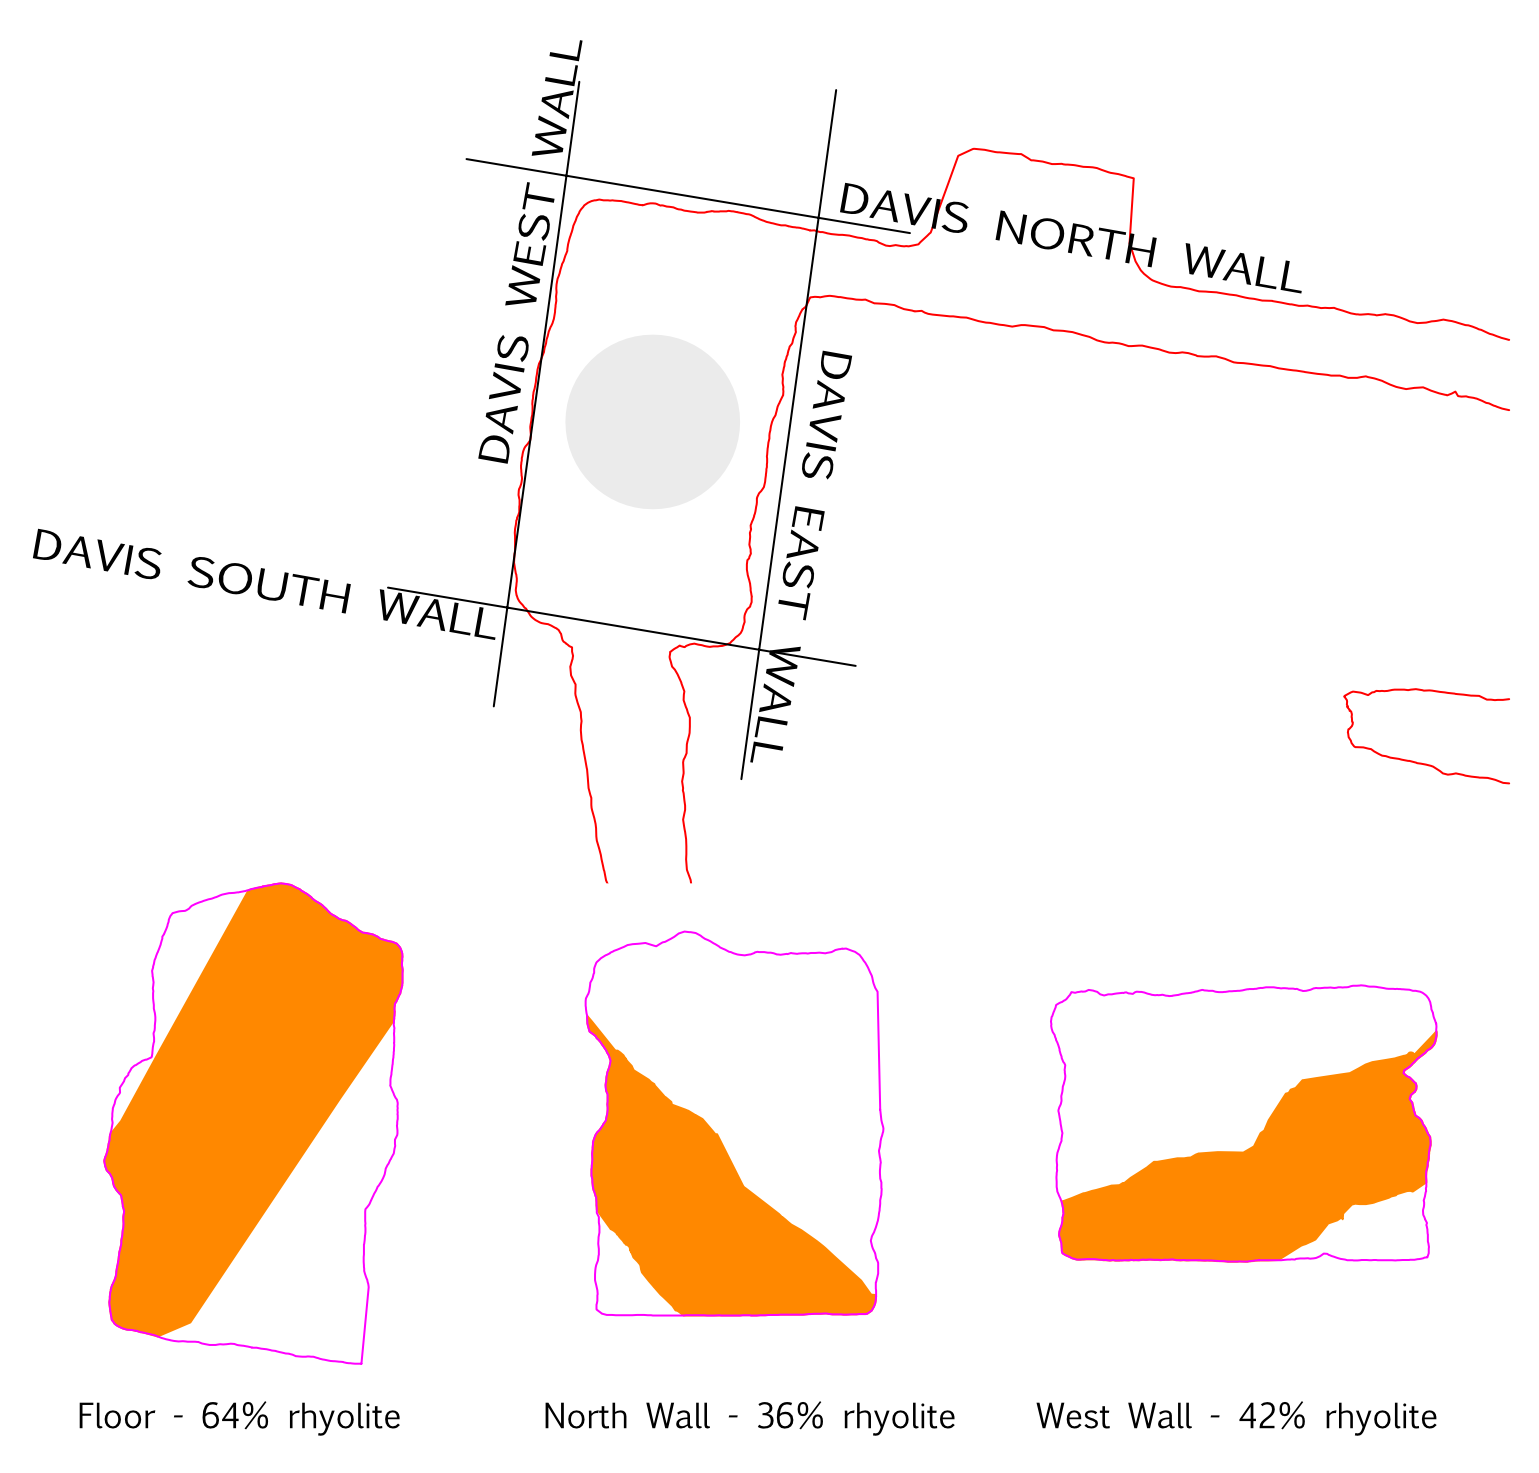
\includegraphics[scale=0.80]{Chapter_3/Figures/Davis_cavern_rhyolite.png}
    \caption[Schematic of the Davis cavern, showing the rhyolite intrusion layers and the position of the water tank with naming conventions.]
    {Diagram of the Davis cavern highlighting the naming conventions of the wall locations and the rhyolite intrusion layers in orange with the estimated percentage coverage of rhyolite. The water tank is marked with a grey circle. The ceiling is estimated at 0\% rhyolite, the south wall at 5\% and the east at 2\% \cite{Heise_2015}. Diagram adapted from \cite{Akerib_2020_gray_measurements}.}
    \label{fig:davis_cavern_walls}
\end{figure}
%

The LZ detectors will be housed within a water tank of height 591 cm and radius 381 cm. Further shielding is provided by 6 octagonal steel plates of 5 cm thickness, inlaid beneath the floor of the water tank with an inverted pyramid hierarchy, directly below the xenon target. The water tank and the steel pyramid are aimed at reducing the environmental radioactivity. Geological and radiometric surveys of the Homestake mine indicate that most rock at the 4,850 level is of the Homestake formation, a metamorphic rock of relatively low uranium and thorium content \cite{Heise_2015}, with additional intrusions of rhyolite segments---an igneous, volcanic, silica-rich rock, with higher natural radioactivity. The estimation of the rhyolite layers as present across the north wall, west wall and the floor are shown in figure (\ref{fig:davis_cavern_walls}). The walls and the ceiling of the cavern is lined with a layer of $\sim$12.7 cm thick sprayed concrete (shotcrete) with a thickness variance of factor two. The floor is covered with a 15 cm low-radioactivity concrete with the exception of two rooms at the end of the cavern, away from the water tank. Prior to this measurement, the radiological contents of the rock formation and construction material were measured with high purity germanium (HPGe) screening; these results are shown in table (\ref{tab:Davis_cavern_sample_screening}). The table also include two recent measurements of samples collected during this measurement. The following sections will summarise the details of the Davis cavern \gray{} measurements, highlighting the experimental setup, detector calibration, data collection and the results. A more detailed overview of these measurements are presented in \cite{Akerib_2020_gray_measurements}.

\begin{table}[]
\centering
\caption{HPGe screening of rock, shotcrete and gravel samples from the Davis cavern laboratory. The first four materials were radioassayed during construction of the Davis cavern and give the average and range for several samples. The latter two samples were taken during the time of the \gray{} measurements. When not stated, overall uncertainties are estimated to be 10–20\%.}
    \label{tab:Davis_cavern_sample_screening}
    \vspace{1mm}
    \renewcommand{\arraystretch}{1.1}
    \begin{tabular}{lcccc}
    \toprule
    
    \multirow{2}{*}{\textbf{Sample}} & %0
    \textbf{} & %1
    \textbf{$^{40}$K} & %2
    \textbf{$^{238}$U} & %3
    \textbf{$^{232}$Th} \\ %4
    
    \textbf{} & %0
    \textbf{} & %1
    \textbf{[Bq/kg]} & %2
    \textbf{[Bq/kg]} & %3
    \textbf{[Bq/kg]} \\ %4
    
    \hline
    \hline
    
    \multirow{2}{*}{\textbf{Homestake}} & ave. & 297 & 2.7 & 1.3 \\
                                        & range & 31--601 & 0.7--9.5 & 1.0--6.5 \\
    \multirow{2}{*}{\textbf{Rhyolite}}  & ave. & 1291 & 108 & 44 \\
                                        & range & 523--2127 & 99--135 & 7.7--61 \\
    \multirow{2}{*}{\textbf{Concrete}}  & ave. & 381 & 27 & 13 \\
                                        & range & 368--393 & 22–27 & 13–14 \\  
    \multirow{2}{*}{\textbf{Shotcrete}} & ave. & 272 & 23 & 12 \\
                                        & range & 127--393 & 22–28 & 8.1–14 \\ 
    \hline
    \textbf{Shotcrete} & - & 220 \pm 30 & 21 \pm 1 & 11.4 \pm 0.4 \\
    \textbf{Gravel} & - & 35.0 \pm 0.6 & 26.3  \pm 0.1 & 1.7 \pm 0.8 \\
    
    \bottomrule
\end{tabular}
\end{table}


\subsection{Experimental Setup}
\label{secsec:experimental_setup}

The \gray{} flux within the cavern was measured using a thallium-doped sodium iodide (NaI) scintillating crystal ($5 \times 5 \times 5 \; \MathText{inches}$) coupled with a PMT. The detector, manufactured by Harshaw, was connected to a NOMAD 92X-P portable \gray{}-spectroscopy unit. The MAESTRO software was used to produce spectra. A total of 130 lead bricks ($8 \times 4 \times 2 \; \MathText{inches}$) were used in three different configurations for direction specific measurements while shielding away \grays{} from unsought directions, providing at least 8 inches of lead on the sides that were not exposed. A picture of the detector and lead brick configurations in which exposures from above and below are shielding is shown in figure (\ref{fig:detector_and_shielding}).
%
\begin{figure}[]
    \centering
    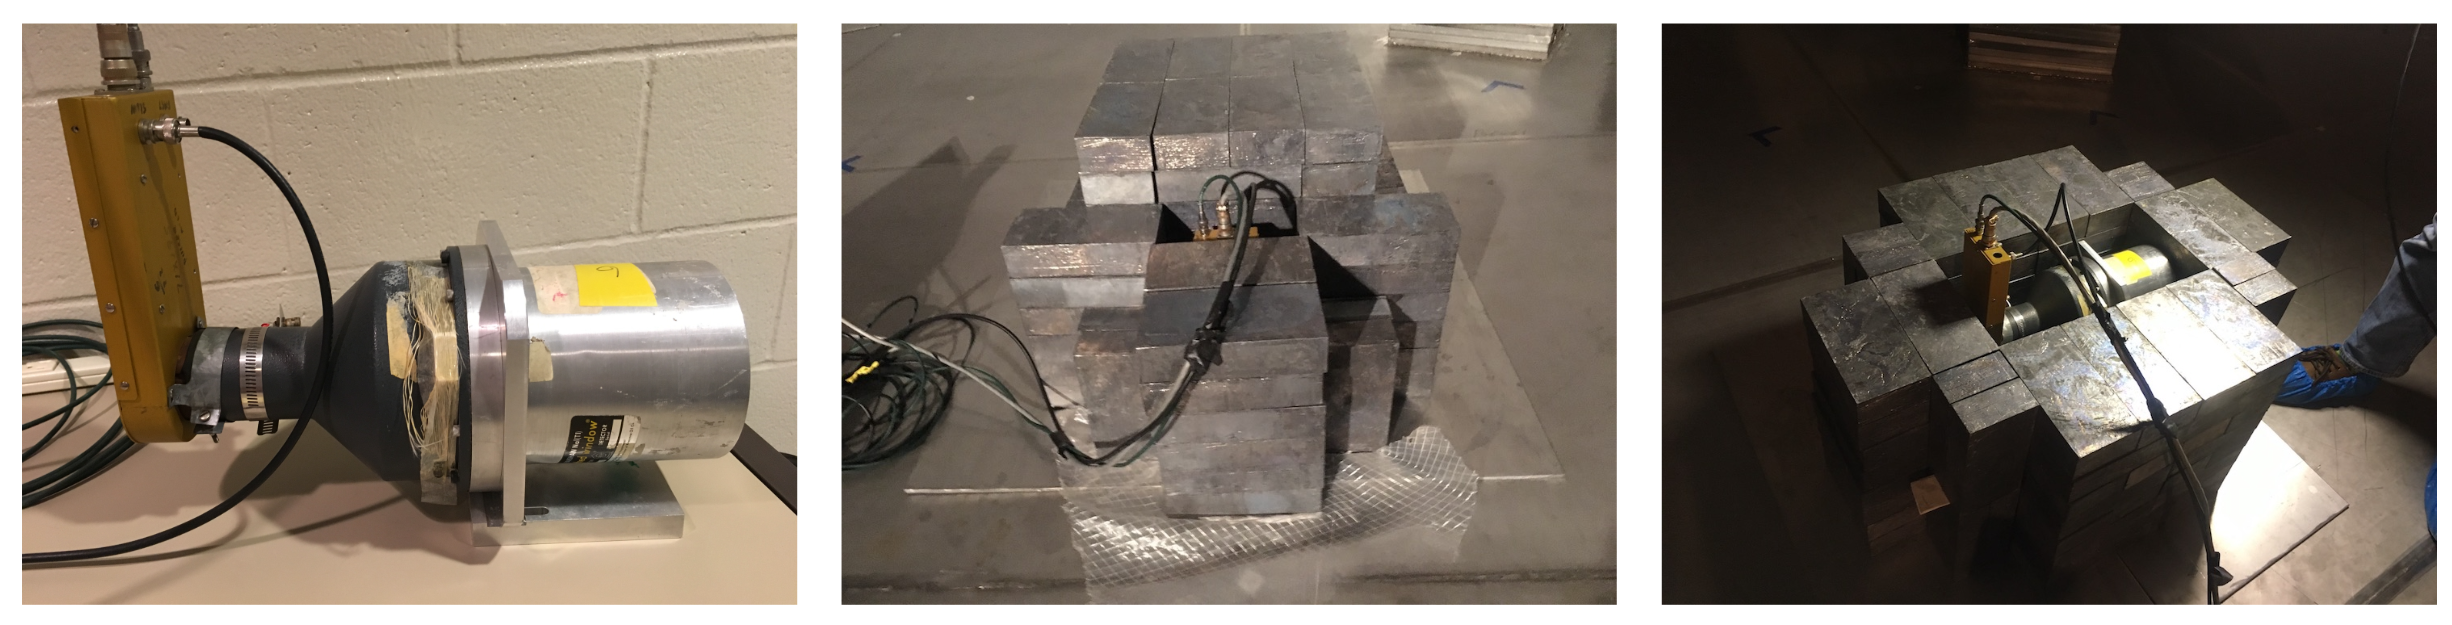
\includegraphics[scale=0.75]{Chapter_3/Figures/Davis_detector_shielding.png}
    \caption[Diagram of the NaI(Tl) crystal detector and the lead shielding used in taking direction specific measurements.]
    {A photograph of the 5-inch NaI(Tl) detector (left), showing the pre-amplifier, PMT and NaI crystal. The right two images are showing the lead shielding configuration in measuring \grays{} from the bottom (centre) and from above (right).}
    \label{fig:detector_and_shielding}
\end{figure}
%

\subsubsection{Detector Calibration and Efficiency}
\label{secsec:calibration_efficiency}


A \CoSZ{} source calibration was performed before each measurement to relate PMT channels to deposited energy and adjust for fluctuations in gain of the NOMAD unit.
Using the 2505 keV peak from \CoSZ{} ensured a dynamic range that fully contained the energy spectrum up to the 2614 keV peak from \TlTZE{}. The detector efficiency and energy resolution were determined by using three calibration sources with their associated energy peaks: \CoSZ{} (1173 keV, 1332 keV, 2505 keV), \CsOTS{} (662 keV) and \TlTZE{} (2614 keV). Each of the energy peaks were fitted with Gaussian's and exponential backgrounds in order to determine the location and resolution of the respective peaks. Calibrations were performed from the same central location within the water tank without shielding. Background measurements from the same location were subtracted from the calibration source spectra to account for \grays{} from the cavern. 

The absolute efficiency of the detector ($\epsilon_{A}$) is given by,
%
\begin{equation}
    \epsilon_{A} = \frac{N(E)}{ATP_{\gamma}(E)}
    \label{eq:detector_eff}
\end{equation}
%
where $N(E)$ is the number of counts in a photopeak of energy $E$, $A$ is the activity of the source, $T$ is the live time and $P_{\gamma}(E)$ is the probability of a single decay producing a \gray{} of energy $E$. $\epsilon_{A}$ is a product of the geometric acceptance due to the fractional solid angle expose of the detector, the \gray{} conversion efficiency within the crystal, and the PMT light collection efficiency. Simulations of calibration sources at varying distances from the detector were performed and source activities were used to calculate the rates in each simulated photopeak. Comparison to data revealed an over-estimation of rates in data, likely as a result of the unaccounted light collection effects in simulations. A correction factor of $0.90 \pm 0.06$ was calculated and applied to further simulations. The resolution ($R$) of each peak was calculated from the full width at half maximum (FWHM) and the energy ($E$) of that peak, using,
%
\begin{equation}
    R = \frac{FWHM}{E} \equiv \frac{\Delta{}E}{E}.
    \label{eq:detector_eff}
\end{equation}
%
The energy dependent resolution scale was then determined by fitting a resolution model, which took into account the light transmission from the scintillating crystal to the photocathode ($\alpha$); statistical fluctuations in photon production, attenuation, conversion and amplification ($\beta$); and the noise contribution ($\gamma$) \cite{An:2016ses}, where,
%
\begin{equation}
    R = \frac{\Delta{}E}{E} \cong \sqrt{\alpha{}^2 + \frac{\beta{}^2}{E} + \frac{\gamma{}^2}{E^{2}}}.
    \label{eq:resolution_model}
\end{equation}
%
The resolution model as applied to the calibrations performed during this measurement are presented in figure (\ref{fig:detector_resolution_fit}) and were later used to correct the true Monte Carlo energy depositions from the simulations in an effort to directly compare with the data from NaI(Tl) detector.
%
\begin{figure}[]
    \centering
    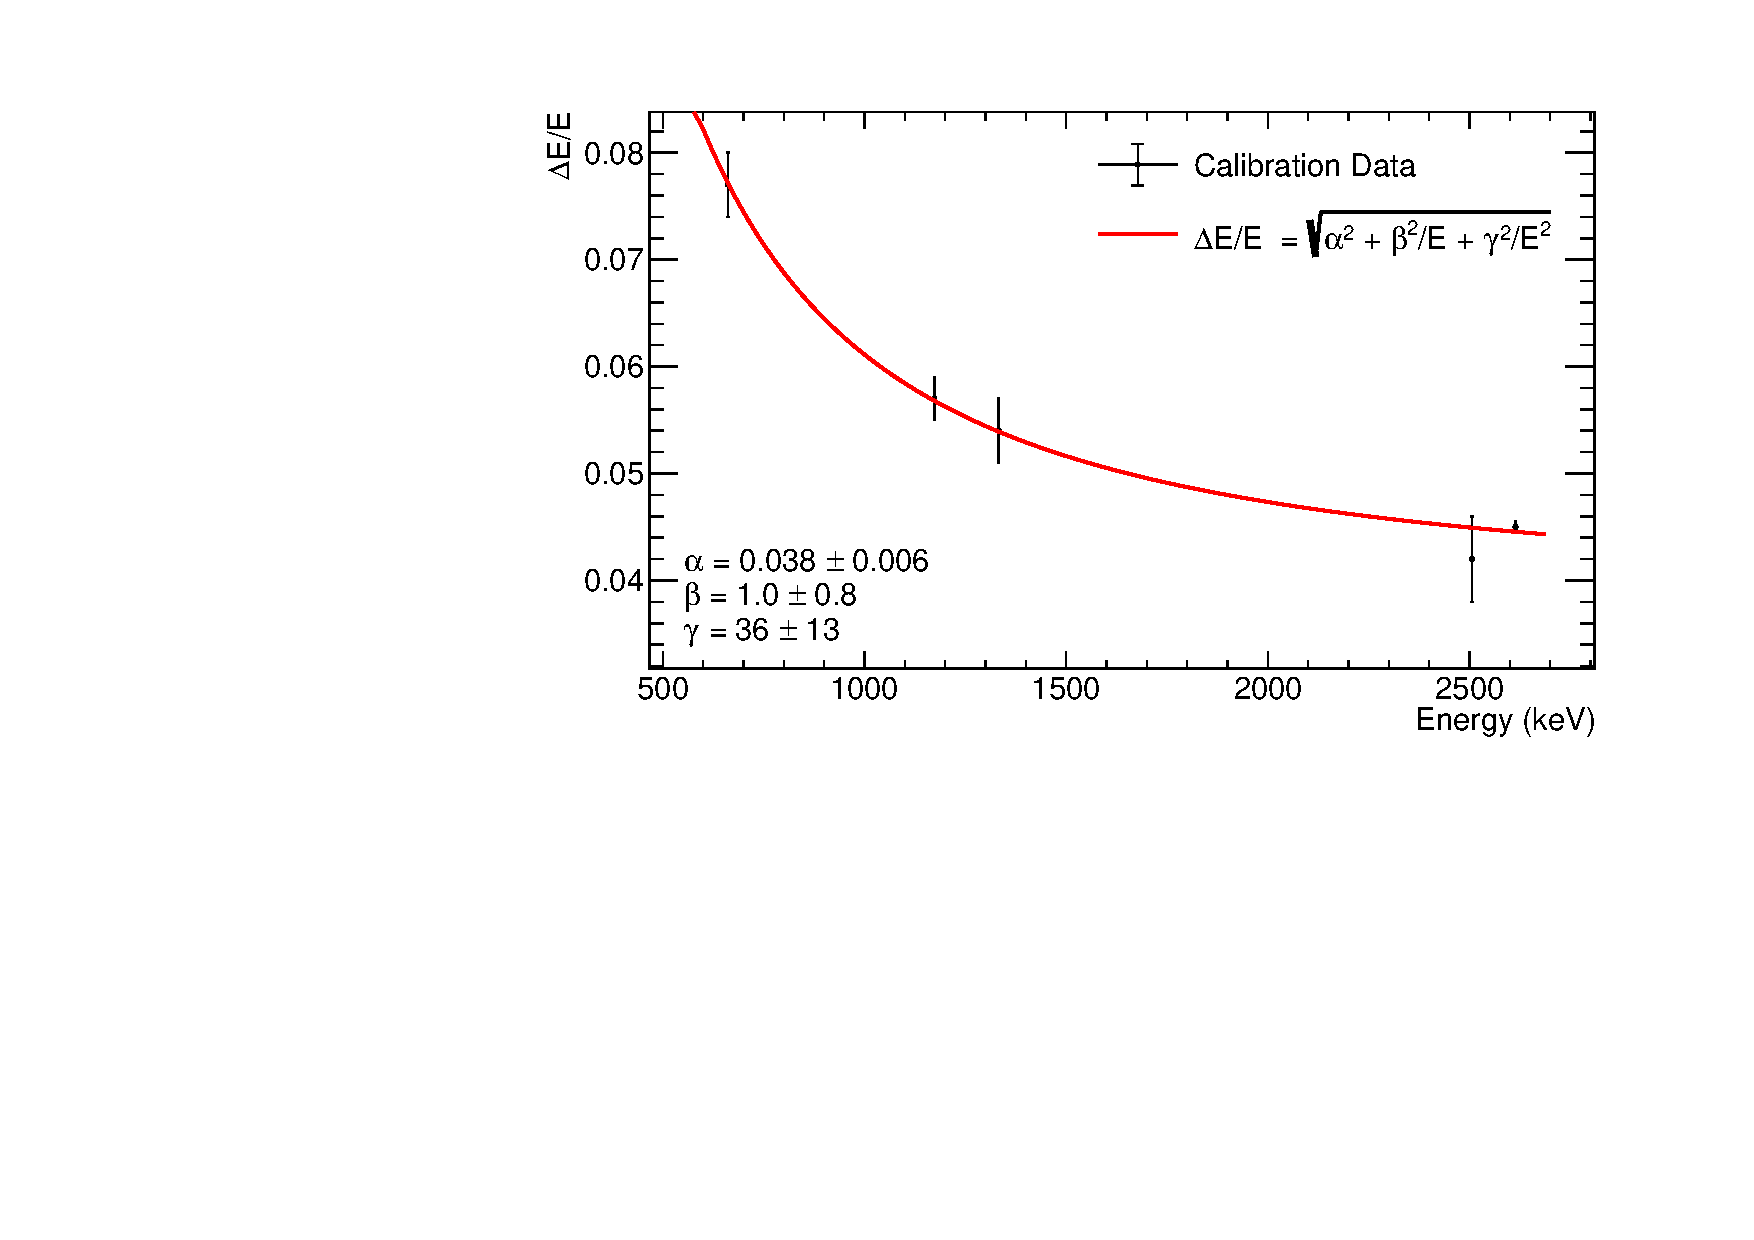
\includegraphics[scale=0.75]{Chapter_3/Figures/NaI_resolution.pdf}
    \caption[Resolution of the NaI(Tl) detector obtained from the calibration source peaks of \CoSZ{}, \CsOTS{} and \ThTTE{}.]
    {Resolution of the NaI(Tl) detector obtained from the calibration source peaks of \CoSZ{}, \CsOTS{} and \ThTTE{}. The fit to data using the resolution model given in equation (\ref{eq:resolution_model}) is also shown.}
    \label{fig:detector_resolution_fit}
\end{figure}
%


\subsubsection{Data Collection}
\label{secsec:data_collection}

A total of nine measurements were conducted to fully map the \gray{} flux within the Davis cavern, focusing primarily on the flux as seen by the water tank as shown in figure (\ref{fig:davis_cavern_layout}). Seven of these were conducted within the water tank; five of which were measurements from the centre of the tank. Locations from the centre consisted of an unshielded measurement (a) and shielded measurements looking down with 30 cm of steel pyramid beneath (f), looking up (g), looking west (h) and looking east (i). The remaining two within the water tank were shielded measurements looking down at the edge (d) and looking down halfway from the centre to the edge with 15 cm of steel pyramid beneath (e). The two measurements outside of the water tank were conducted unshielded in the Upper Davis above the water tank (b) and on the floor of the counting room (c). Measurements looking down within the water tank were aimed at measuring the effectiveness of the steel pyramid, whereas those facing the walls aimed at assessing the asymmetry due to the presence of rhyolite.
%
\begin{figure}[]
    \centering
    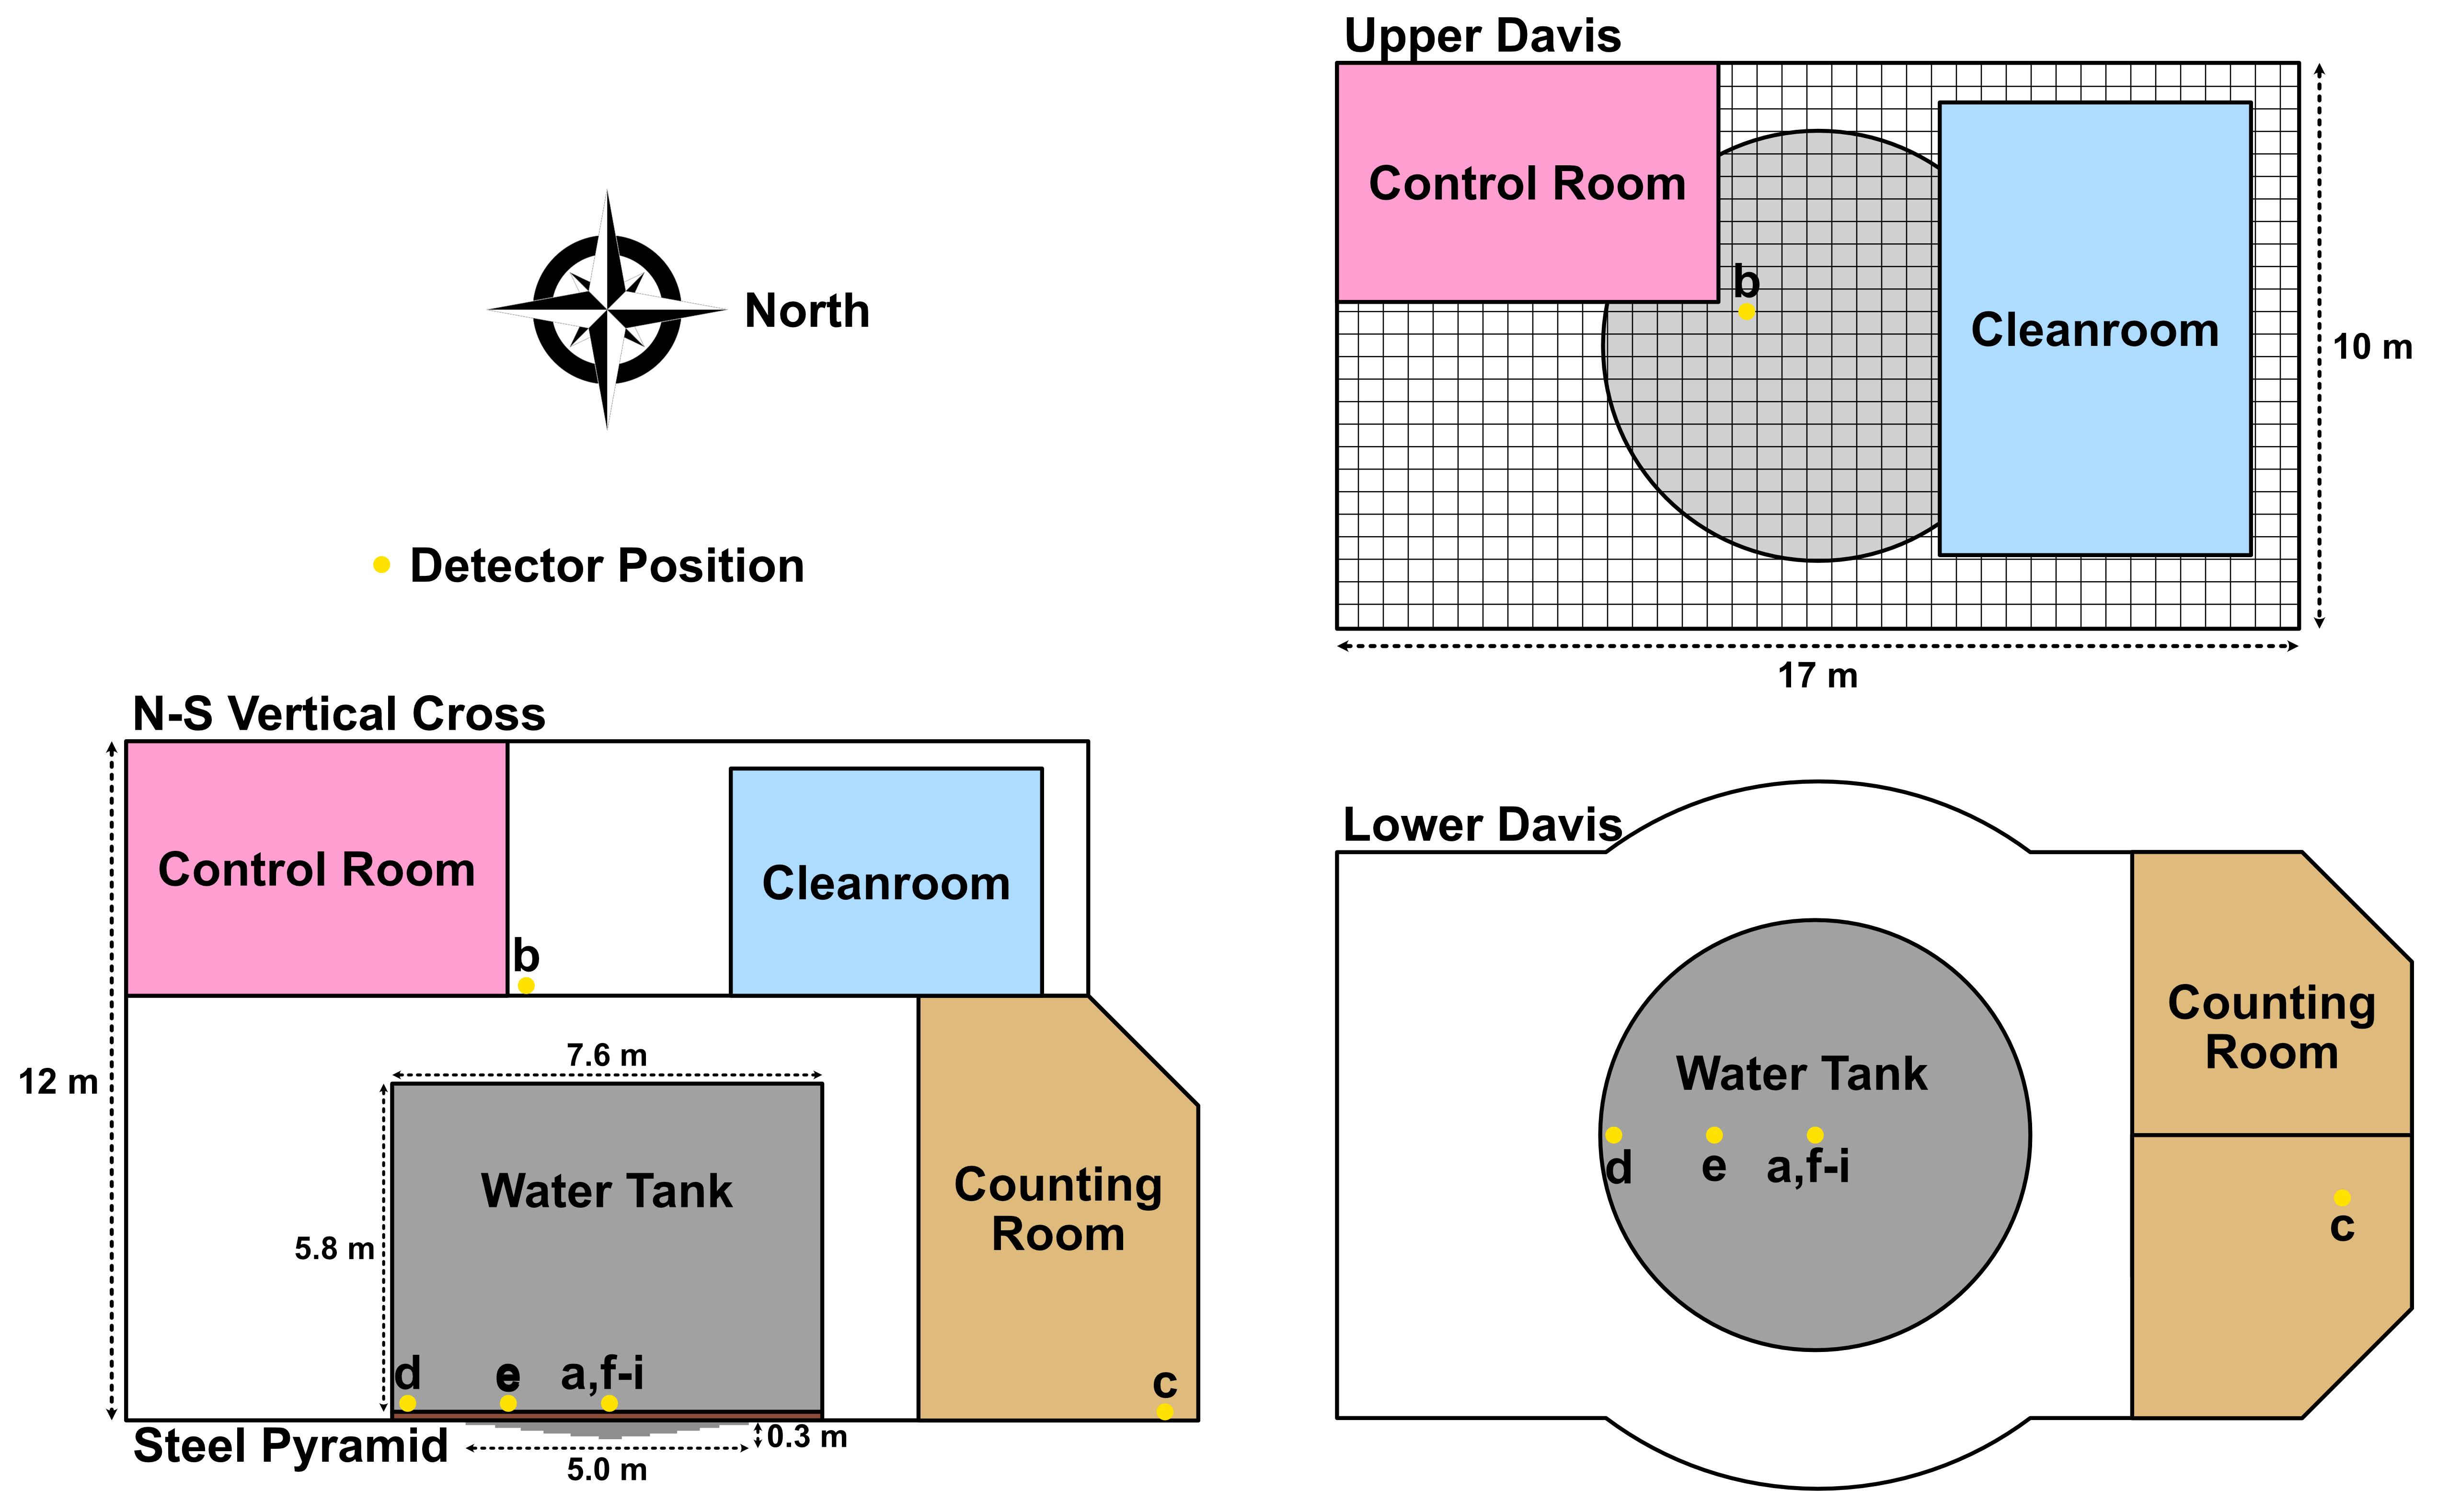
\includegraphics[scale=0.085]{Chapter_3/Figures/Davis_cavern_diagram.jpg}
    \caption[Schematic layout of Davis cavern at the time of the measurement, highlighting key dimensions and the measurement positions with yellow dots.]
    {Schematic layout of Davis cavern at the time of the measurement, highlighting key dimensions and the measurement positions with yellow dots. The labels of the positions directly map to measurement results within tables (\ref{tab:Davis_cavern_measurement_details}).}
    \label{fig:davis_cavern_layout}
\end{figure}
%
%
\begin{figure}[t!]
    \centering
    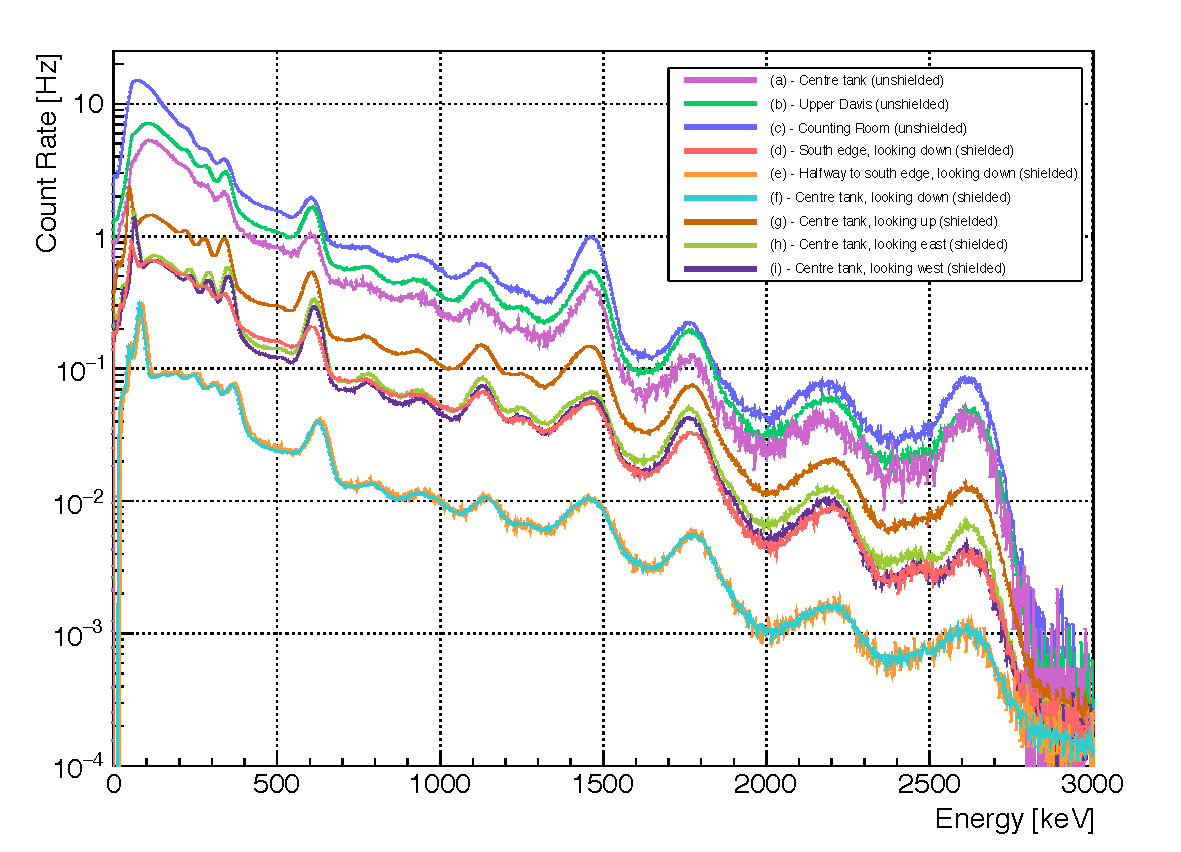
\includegraphics[scale=0.80]{Chapter_3/Figures/Davis_cavern_spectra.pdf}
    \caption[The energy spectra for all nine measurements labeled with their corresponding positions in the energy range 0–3000 keV.]
    {The energy spectra for all nine measurements labeled with their corresponding positions in the energy range 0–3000 keV.}
    \label{fig:davis_cavern_spectra}
\end{figure}
%
The measured energy spectra from all of the 9 positions are shown in figure (\ref{fig:davis_cavern_spectra} and their integrated rates, along with differing exposure times and measured ambient radon levels are summaries in table (\ref{tab:Davis_cavern_measurement_details}). The lowest rates observed are from two measurements inside of the water tank, at the centre (f) and halfway to the edge (e), both facing down. Despite the much longer exposure time for (f) and the differences in the thickness of pyramid shielding below, the rates observed for these two measurements are comparable. This suggests that the rates observed in these positions are intrinsic to the experimental setup---essentially a background of the experiment, as NaI(Tl) crystals and PMTs are known to have intrinsic \KFZ{}, \UTTE{} and \ThTTT{} contamination \cite{Kim:2014toa}. Measurements facing east and west are comparable in rate, signalling no significant asymmetry due to the difference in rhyolite intrusion within the walls. This may imply that the difference observed in the directional flux ($\sim$ 10\%) may be due to unevenness in shotcrete thickness since the shotcrete is approximately 10 times more radioactive than the Homestake formation in \UTTE{} and \ThTTT{}. The measurement at the edge of the water tank looking down (d) does show a higher rate than both (e, f) suggesting that the steel pyramid is in fact reducing the flux from below. The rates were highest in the east counting room, followed by the upper level of the Davis cavern and the centre of the water tank---all unshielded.

Decays from the \RnTTT{} sub-chain make up a majority of the \grays{} in the \UTTE{} chain, hence the activity of radon within the cavern air must be considered. The average radon concentration taking into account seasonal dependence in the Davis Campus is expected to be within 150--310 Bq/m$^3$ \cite{Heise_2015}. However, unusually high radon levels were recorded (measured with an AlphaGuard detector) some of the days, possibly as a result of the air flow and air circulation fluctuations within the mine drift. The recorded levels from an area outside the main entrance to the cavern known as the common corridor during each dataset are also shown in table (\ref{tab:Davis_cavern_measurement_details}). Although there may be uncertainties due to the differences in location, the concentrations were significant enough that \grays{} from airborne-radon was included in the analysis.

\begin{table}[h]
\centering
\caption{Dates, live times, radon concentrations and integrated. count rates for each measurement position. The centre of tank measurements were shielded from all directions except the intended direction as stated. Stated uncertainties are Poisson counting errors. Data adapted from \cite{Akerib_2020_gray_measurements}.}
    \label{tab:Davis_cavern_measurement_details}
    \vspace{1mm}
    \renewcommand{\arraystretch}{1.1}
    \begin{adjustbox}{width=\textwidth}
    \begin{tabular}{lcccccc}
    \toprule
    
    \multirow{2}{*}{\textbf{Measurement Position}} & %0
    \multirow{2}{*}{\textbf{Label}} & %1
    \multirow{2}{*}{\textbf{Date}} & %2
    \textbf{Live time} & %3
    \textbf{Ave. \RnTTT{} Act.} & %4
    \textbf{Rate (total)} & %5
    \textbf{Rate (>200 keV)} \\ %6  
    
    \textbf{} & %0
    \textbf{} & %1
    \textbf{} & %2
    \textbf{[hours]} & %3
    \textbf{[Bq/m$^{3}$]} & %4
    \textbf{[Hz]} & %5
    \textbf{[Hz]} \\ %6
    
    \hline
    \hline
    
    Centre of tank (unshielded) & a & 24/10/17 & 4.0 & 422 \pm 34 & 595.7 \pm 0.2 & 386.0 \pm 0.2 \\
    Upper Davis (unshielded) & b & 26/10/17 & 3.6 & 868 \pm 222 & 794.4 \pm 0.2 & 512.0 \pm 0.2 \\
    Counting Room (unshielded) & c & 26/10/17 & 2.1 & 929 \pm 70 & 1355.0 \pm 0.4 & 750.9 \pm 0.3 \\
    South Edge, looking down & d & 16/10/17 & 18.2 & 358 \pm 80 & 94.17 \pm 0.04 & 64.40 \pm 0.03 \\
    Halfway to South Edge, looking down & e & 17/10/17 & 17.9 & 336\pm55 & 17.15 \pm 0.02 & 10.70 \pm 0.01 \\
    Centre of tank, looking down & f & 19/10/17 & 117.0 & 500 \pm 155 & 16.715 \pm 0.006 & 10.427 \pm 0.005 \\
    Centre of tank, looking up & g & 18/10/17 & 20.2 & 372 \pm 76 & 203.57 \pm 0.05 & 139.0 \pm 0.04 \\
    Centre of tank, looking west & h & 24/10/17 & 17.3 & 359 \pm 37 & 95.11 \pm 0.04 & 51.77 \pm 0.03 \\
    Centre of tank, looking east & i & 25/10/177 & 22.3 & 316 \pm 46 & 106.33 \pm 0.4 & 59.14 \pm 0.03 \\
    
    \bottomrule
    \end{tabular}
    \end{adjustbox}
\end{table}


\subsection{Simulation \& Analysis}
\label{secsec:simulations_analysis}

Simulations of the \gray{} background within Davis cavern are performed using the \textsc{BACCARAT} framework, a \textsc{GEANT4} (v.10.03) \cite{Geant4} package developed primarily for LZ background simulations---detailed further in section (\ref{sec:LZ_simulation_framework}). Electromagnetic processes were modelled using the \textit{G4EMLivermorePhysics} class, a sub-package that models interactions of \gray{} and electron cross-sections \cite{osti_295438, osti_5691165}, focusing on low energy processes, such as Rayleigh, Compton scattering, bremsstrahlung and the photoelectric effect. 

A custom geometry featuring the cavern, steel pyramids, water tank and the NaI detector was created, with additional shielding geometry, taking into account the three different configurations. The cavern was modelled as a cuboid to have internal dimensions of $20 \times 14 \times 12$ m; slightly larger than stated in figure (\ref{fig:davis_cavern_layout}) to account for the unevenness of the cavern walls. The cavern walls were defined as a mixture of oxides, primarily SiO$_{2}$, Al$_{2}$O$_{3}$, FeO and water \cite{Mei_2010}. Decays from the \UTTE{} and \ThTTT{} chains and the \KFZ{} decay were all initiated within a 30 cm thick layer of material surrounding the cavern. The \UTTE{} and \ThTTT{} chains were simulated using an event generator developed for LZ background simulations. The generator assumes secular equilibrium and initiates a chain of decays beginning at \UTTE{} or \ThTTT{} and ending at the stable \PbTZS{} or \PbTZE{}, initiating all of the \alpha, \beta and \gamma-decays for the entire chain with correct  energies and branching ratios. Moreover, the \RnTTT{} chain was also simulated within the cavern air and the water tank to account for the elevated levels of radon at the time of the measurement and the rates normalised using the measured concentrations. The simulated dataset recorded energy depositions of the \grays{} within the NaI crystal and further smeared the data using a Gaussian function; accounting for the energy resolution by using the resolution model fit to calibration data as shown in figure (\ref{fig:detector_resolution_fit}).

An equivalent of 1 Bq/kg was simulated to calculate the activity necessary for each isotope of interest within the cavern walls to reproduce the rates observed in data. The simplest technique to scale the simulations to data was by fitting Gaussian's to each of the prominent peaks at 1461 keV (\KFZ{}, BR: 10.66\%), 1764 keV (\BiTOF{}, BR: 15.30\%) and 2614 keV (\TlTZE{}, BR: 99.75\%). Focusing on the photopeaks was to select those \grays{} produced near to the surface of the cavern to reduce the effects of the Compton background leaking into each peak. The analysis further focused on \grays{} with energies of 1400 keV or above where the Compton background is less dominate. 
%
\begin{figure}[t!]
    \centering
    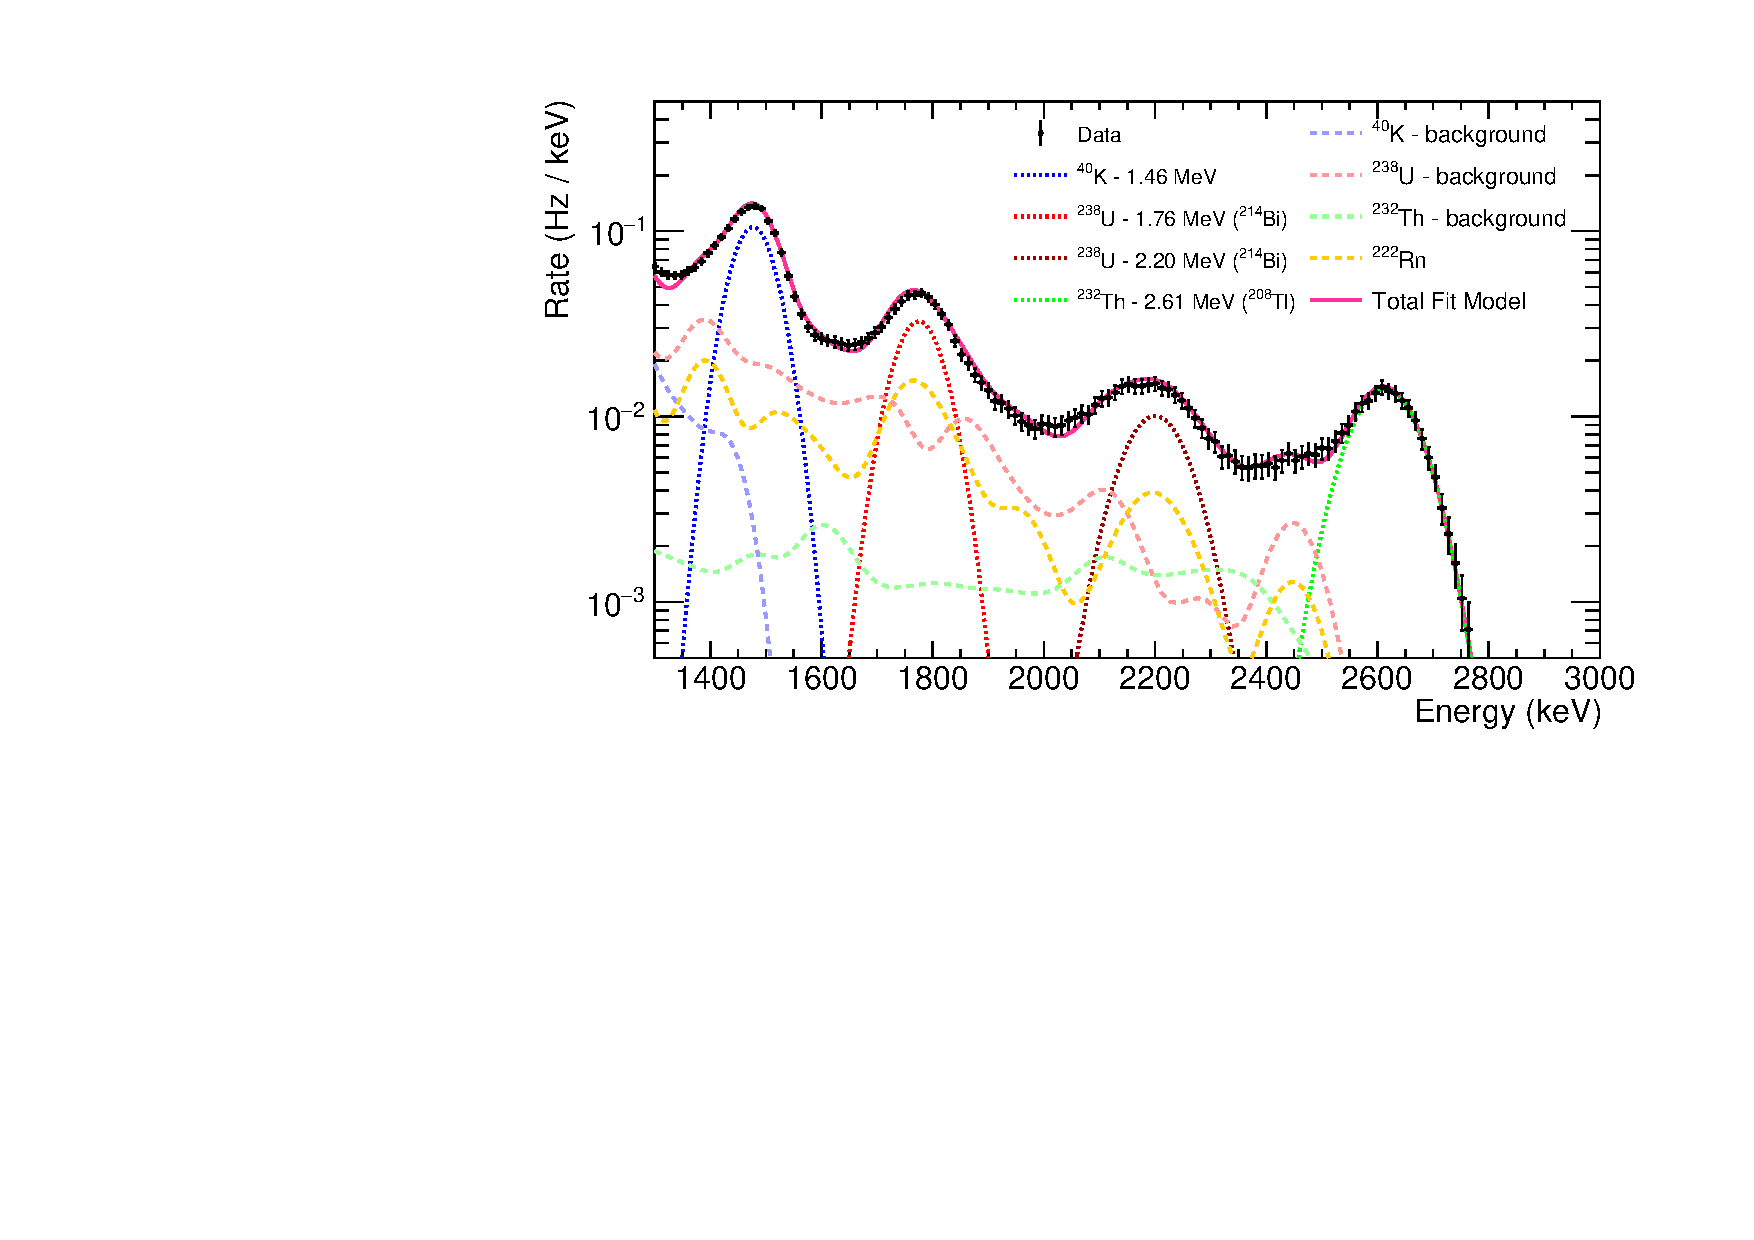
\includegraphics[scale=0.80]{Chapter_3/Figures/Cavern_peak_fits.pdf}
    \caption[Fitted energy spectra for position (a) showing the 1461 keV \KFZ{} peak, 1764 keV and 2204 keV peaks from \UTTE{} and the 2614 keV peak from \ThTTT{}, with background contributions.]
    {Fitted energy spectra for position (a) showing the 1461 keV \KFZ{} peak, 1764 keV and 2204 keV peaks from \UTTE{} and the 2614 keV peak from \ThTTT{}, with background contribution PDFs from less dominant lines, air-borne radon and Compton scattering. Diagram adapted from \cite{Akerib_2020_gray_measurements}.}
    \label{fig:davis_cavern_spectra_fit}
\end{figure}
%
The Compton backgrounds overlaying the peaks of interest contain \grays{} from all energies and peaks from the uranium and thorium chains. To model for this, a background probability distribution function (PDF) was created using the simulated spectra of each isotope with the prominent lines removed and signal PDFs were produced from Gaussian functions with widths constrained within error bars obtained from the resolution function. A background PDF was also constructed for the \RnTTT{} decay chain \grays{} to account for the ambient radon. The fit was constrained by fixing the branching ratio of \BiTOF{}, allowing the rate from radon to  float within 20\% uncertainty due to location dependent uncertainties and the peak-to-continuum ratio was constrained to float within 20\% of the simulated value for each contribution. An example of the fit to the unshielded data taken in the centre of the water tank is shown in figure (\ref{fig:davis_cavern_spectra_fit}).

The corresponding activity of \UTTE{}, \ThTTT{} and \KFZ{} within the wall shell was calculated for each measurement position by using the three isotopic decays by comparison to the simulated rates. The activity for each isotope (denoted by the subscript \textit{i}) and measurement position (denoted by the subscript \textit{p}) is given by
%
\begin{equation}
    A_{i,p} = \frac{R_{i,p} - R^{bkg}}{\epsilon{}R^{sim}_{i,p}},
    \label{eq:resolution_model}
\end{equation}
%
where $R_{i,p}$ is the signal peak in data as determined by the Gaussian fit, $R^{bkg}$ is the internal background rate of the setup as measured in (e,f), \epsilon{} is the aforementioned efficiency correction determined from calibration and $R^{sim}_{i,p}$ is the simulation normalisation factor calculated using,
%
\begin{equation}
    R^{sim}_{i,p} = \frac{N_{i,p}}{N^{tot}_{i,p}B_{p}M}.
    \label{eq:resolution_model}
\end{equation}
%
Here $N_{i,p}$ is the raw number of counts in a given peak for isotope \textit{i} and position \textit{p}, $N^{tot}_{i,p}$ is the total number of events simulated, $B_{p}$ is the event biasing multiplicative factor and $M$ is the mass of the simulated shell. The event biasing multiplicative factor is as a result of a biasing technique used to increase \gray{} statistics hitting the detector by saving \grays{} on a predefined surface and then propagating a larger quantity onward with the same momentum in a second simulation. The fit results for each peak in activity $A_{i,p}$ are given in table (\ref{tab:Davis_cavern_results}).


\subsection{Results \& Discussion}
\label{secsec:results_discussion}

In assuming that each measurement is an independent observation of the same flux within the cavern, the averaged activities across the positions of interest result in $220 \pm 60 \; \MathText{Bq/kg}$ of \KFZ{}, $29 \pm 15 \; \MathText{Bq/kg}$ of \UTTE{} and $13 \pm 3 \; \MathText{Bq/kg}$ of \ThTTT{}. The results from the HPGe screening of the shotcrete samples taken during the measurement indicate activities of $220 \pm 30 \; \MathText{Bq/kg}$ of \KFZ{}, $21 \pm 1 \; \MathText{Bq/kg}$ of \UTTE{} and $11.4 \pm 0.4 \; \MathText{Bq/kg}$ of \ThTTT{}, all of which are in good agreement within uncertainties with the results of this analysis. 

\begin{table}[h]
\centering
\caption
[Results from the fits on the three signature peaks from the \KFZ{}, \UTTE{} and \ThTTT{} decay chains.]
{Results from the fits on the three signature peaks from the \KFZ{}, \UTTE{} and \ThTTT{} decay chains. The best fit activities, $A_{m}$, of the resultant activity within the wall shell from each measurement are given for the positions of interest. The uncertainties are from fit results only, but systematic uncertainties are expected from the simplified simulation geometry. The average values are show at the bottom with their standard deviations. Data adapted from \cite{Akerib_2020_gray_measurements}.}
    \label{tab:Davis_cavern_results}
    \vspace{1mm}
    \renewcommand{\arraystretch}{1.1}
    \begin{adjustbox}{width=\textwidth}
    \begin{tabular}{lc|ccc}
    \toprule
    
    \multirow{2}{*}{\textbf{Measurement Position}} & %0
    \textbf{Label} & %1
    \textbf{$^{40}$K (1461 keV)} & %2
    \textbf{$^{238}$U (1764 keV)} & %3
    \textbf{$^{232}$Th (2614 keV)} \\ %4
    
    \textbf{} & %0
    \textbf{} & %1
    \textbf{ \textit{A$_{p}$} [Bq/kg]} & %2
    \textbf{ \textit{A$_{p}$} [Bq/kg]} & %3
    \textbf{ \textit{A$_{p}$} [Bq/kg]} \\ %4
    
    \hline
    \hline
    
    Centre of tank (unshielded) & a & 285 \pm 1 & 36.9 \pm 0.4 & 15.2 \pm 0.14 \\
    Upper Davis (unshielded) & b & 135 \pm 4 & 10.4 \pm 0.2 & 8.8 \pm 0.1 \\
    Counting Room (unshielded) & c & 264 \pm 1 & 18 \pm 0.2 & 12.2 \pm 0.2 \\
    South Edge, looking down & d & 182 \pm 2 & 31.4\pm0.2 & 16.7 \pm 0.1 \\
    Centre of tank, looking up & g & 214 \pm 1 & 48.4 \pm 0.2 & 9.5 \pm 0.1 \\
    
    \hline
    
    Averaged activities & - & 220 \pm 60 & 29 \pm 15 & 13 \pm 3 \\
    
    \bottomrule
    \end{tabular}
    \end{adjustbox}
\end{table}

However, large variations are observed when taking a closer look at the activities from each measurement; although not fully understood, this could be a result of multiple factors. The first of these could be as a result of the uncertainty of the radon concentration within the cavern. The activity of radon used in the simulation were measured outside of the Davis cavern and without a model of the airflow into the cavern, it is difficult to account for this uncertainty. Since most of the \grays{} are emitted from the \RnTTT{} sub-chain, this uncertainty is expected to account for the observed large variations. Furthermore, the simulation does not take into account some of the key features of the cavern, such as the steel grating diving the two floors, walls of the counting room and the control room. Lastly, the variation in different activities may indicate towards a non-uniformity in the concentrations of each isotope spatially within the cavern walls, especially in places where the fluctuations in Shotcrete thickness may lead to \grays{} leaking from the highly active non-uniform Rhyolite layers. Despite the variations between measurements, the results can be used to estimate the background contribution from the Davis cavern for the LZ dark matter experiment.


  \chapter{Radon Emanation in LZ}
\label{chap:chap4}

The discovery of radon dates back to 1900, when Friedrich Ernst Dorn reported results showing the emanation of a radioactive gas from radium compounds \cite{PARTINGTON1957}. Since then we now know that all isotopes of radon are radioactive, and only five are found in nature. With advancements in reducing cosmogenic and detector backgrounds in low-background dark matter experiments, emanation of radon is now the largest background contributor for the WIMP search ROI \cite{akerib2018projected}. The focus of this chapter is to highlight the relevance of radon for the LZ experiment; detailing the radon screening campaign of LZ, predominantly focusing on the work done at UCL and presenting the total expected radon emanation of the LZ detector.


%%------------------------------$$
\section{Overview}
%%------------------------------$$

Radon is a chemical element with an atomic number 86 found in the 6\textsuperscript{th} period of the noble gases. It occurs naturally in trace amounts in the radioactive decay chains through which uranium and thorium decay into lead and various other short-live radioactive elements, as shown in figure \ref{fig:u_238_and_th_232}. It is found as a monatomic gas due to its full outer valence shell with solely radioactive isotopes. A consequence of its inert nature is that radon often exhibits a long diffusion length through solids. Its inert nature makes it extremely difficult for any filtration via chemical means, hence most removal attempts are achieved through physical methods. 

Radon is a colourless and odourless gas under standard temperature and pressure (STP). Its melting and boiling points are comparatively high for a noble gas, at -71$^{\circ}$C and -61.7$^{\circ}$C, respectively, and is densest of the noble gases with a density of 9.7 kg/\cubicmeter{} at standard temperature and pressure. Activity of radon can vary substantially due to the composition of the environmental conditions. Typical atmospheric activities are $\sim10$ Bq/\cubicmeter{} and around 30--50 Bq/\cubicmeter{} for indoor environments. In underground laboratories, such as SURF, the activities can vary between 200--1000 Bq/\cubicmeter{} \cite{Heise_2015}, with significant fluctuations due to the variance in ventilation rate of the underground facility. Salt mines report amongst the lowest activities of all underground laboratories, such as the Boulby mine with $\sim3$ Bq/\cubicmeter{} \cite{scovell_boulby}. 

The significance of the radon background in LZ motivates a need for material screening and selection. Although \gray{} spectroscopy can be useful in measuring the bulk activities of \UandTe{} and \UandTl{}, without material specific radon diffusion coefficients, its difficult to understand the radon emanation rate of materials purely from \gamma-spectroscopy. LZ utilises four facilities for radon emanation screening, built to collect and directly measure the emanated radon from screened samples, leading to a more accurate result in constructing the radon-induced background rate. The following sections will focus primarily on the operation of the UCL facility, highlighting important results measured for the LZ experiment. Thereafter, summaries of the other facilities will be detailed and the total radon budget of LZ will be taken into account. 

%%------------------------------$$
\section{Radon Backgrounds in LZ}
\label{sec:radon_and_lz}
%%------------------------------$$

\subsection{Origin of Radon Emanation}
\label{secsec:radon_origins}

All isotopes of radon are radioactive and only five are naturally found in minute quantities in nature. Those of interest for the LZ background model and often other low background experiments in search for WIMP dark matter or \neutrinolessDoubleBeta{} experiments are \RnTTT{} ($\tau_{1/2}=3.8232 \; d$) from the \UTTE{} decay chain and \RnTTZ{} ($\tau_{1/2}=55.8 \; s$) from the \ThTTT{} decay chain; hereafter called radon and thoron, respectively. Due to the long lifetime of their progenitor isotopes, radon and thoron are produced at a near-constant rate within detector material. They can then diffuse out, mixing with the GXe or LXe, and inevitably decaying within the active volume of the detector. The emanation rate of a material can be broken down into two parts: emanation due to recoiling radon atoms (i.e. \RnTTT{} or \RnTTZ{}) from their subsequent radium parent isotopes (i.e. \RaTTS{} or \RaTTF{}), $E_{recoil}$, and emanation due to diffusion, $E_{diffusion}$. The total emanation rate is then given by the sum total of the two components,
%
\begin{equation}
    E_{tot} = E_{recoil} + E_{diffusion}.
    \label{eq:radon_emanation}
\end{equation}
%
Emanation due to diffusion can vary drastically depending on chemical and lattice structures of a material, density, surface roughness, and temperature; whereas the emanation from recoiling radon atoms depend heavily on the density of the material and the kinetic energy carried by the radon atom from the subsequent radium decay. \RnTTT{} (\RnTTZ{}) recoils with a kinetic energy of 86.26 (103.4) keV, with recoil ranges varying between 20--30 nm for materials such as Zircon or Quartz, and 60--65 \micro{}m for air and water \cite{radon_emanation_modeling}. The diffusion length, $L(m)$, is given as, 
%
\begin{equation}
    L(m) = \sqrt{D/\lambda},
    \label{eq:radon_emanation_diffusion}
\end{equation}
%
where $D$ is the diffusion coefficient and $\lambda{}$ the decay constant. A diffusion coefficient of $10^{-24} \; \MathText{m}^2 \; \MathText{s}^{-1}$ corresponds to 0.7($9 \times{} 10^{-3}$) nm for \RnTTT{} (\RnTTZ{}). Due to the much shorter half-life of \RnTTZ{}, the emanation of \RnTTZ{} in almost all material used in LZ is assumed to be dominated by the recoil emanation, whereas for \RnTTT{} both factors are assumed to play a role in the total emanation rate, with the ratio $E_{diffusion}/E_{recoil}$ expected to be suppressed in colder temperatures. 


\subsection{Radon Emanation Background in LZ}
\label{secsec:radon_in_lz}

In LZ, the material and surfaces of interest for radon emanation are those that are in direct contact with either GXe or LXe. Upon emanation, due to its relatively long half-life, \RnTTT{} is expected to mix homogeneously within the active volume. Although the same assumption is made for \RnTTZ{}, due to its much shorter half-life and diffusion length, a significant suppression is expected relative to \RnTTT{}, hence the assumed activity for \RnTTZ{} is 5\% that of the expected activity of \RnTTT{} as measured and estimated by radon screening. This assumption is made as a conservative measure upon measurements from the LUX detector, as its extremely difficult to screen for \RnTTZ{} emanation due to its short half-life.

The background from radon emanation for the WIMP search ROI is dominated by the ground-state to ground-state or \textit{naked} \beta-emission from the \PbTOF{} progeny of the \RnTTT{} sub-chain, as it decays to \BiTOF. This results in a uniform ER background with a \beta-spectrum of up to 1019 keV. Similarly, the background from \RnTTZ{} is from the \textit{naked} \beta-emission from \PbTOT{}, as it decays into \BiTOT{} with a \beta-spectrum of up to 569.9 keV. The remaining decays from the sub-radon chain are either too high in energy---in the case of \alpha-decays---or decay with a subsequent particle, i.e., a \gray{} or an \alpha particle, and hence can be vetoed via coincidence tagging, as such is the case for the \beta-decay of \BiTOF{}, which is subsequently followed by the \alpha-decay of \PbTOF{} with a half-life of $\tau{} = 162.3 \; \MathText{\micro{}s}$ \cite{radiogenic_muon_lux,Araujo:2011as}. For the WIMP search RIO, the tagging efficiency for \BiPoTOF{} and \BiPoTOT{} is near-optimal, as the \alpha{} particle falls into the same trigger window as the \beta{}. Another isotope to consider is \BiTOZ{}, however due to its relatively long half-life, most of the \BiTOZ{} is expected to be captured by the circulation system; \BiTOZ{} due on TPC surfaces due to plate-out is considered in \ref{chap:chap3}. The details of the decay of each isotope in the radon and thoron sub-chain are summarised in table \ref{tab:radon_decay_chains}.

Radon emanation requirements for the LZ experiment are predetermined to ensure that the background due to radon does not significantly dominate over the irreducible \textit{pp} solar neutrino background, in order to maximise the WIMP search sensitivity in the low mass region. A total of 20 mBq of \RnTTT{} activity is set as the threshold, of which 13.4 mBq is within the 7 tonnes of the active volume and 11.2 mBq in the 5.6 tonne fiducial volume. The radon emanation background from the latest projections account to $\sim66\%$ of the projected ER background in the WIMP search region of interest in LZ~\cite{akerib2018projected}, predominantly from a projected \RnTTT{}(\RnTTZ{}) specific activity of $1.83(0.09) \; {\micro\becquerel\per\kilogram}$ that corresponds to approximately \SI{18.3(0.9)} mBq in the 10 tonnes of xenon. The methodology used in estimating the projected activity of \RnTTT{} and \RnTTZ{} will be highlighted in later sections. 

\begin{table}[h]
\centering
\caption{Details of isotopes in the \RnTTT{} and \RnTTZ{} decay chains, starting from \RaTTS{} (upper) and \RaTTF{} (lower), down to \PoTOF{} and \PoTOT{}, respectively. The table also details the progenitor isotopes of the radon and thoron chains; \UTTE{} and \ThTTT{}.}
\label{tab:radon_decay_chains}
\vspace{1mm}
\renewcommand{\arraystretch}{1.2}
    \begin{tabular}{llllll}
    
    \textbf{Isotope} & %1
    \textbf{Decay} & %2
    \textbf{Q-value [MeV]} & %3
    \textbf{$\tau_{1/2}$} & %4
    & %4
    \textbf{Daughter} & %5
    
    \hline
    \hline
    
    \UTTE{}	    & \alpha{}      & 4.270     & 4.47($10^{9}$)  & y     & - \\ 
    \vdots      & \vdots        & \vdots    & \vdots          &       & \vdots \\ 
    \RaTTS{}	& \alpha{}      & 4.871     & 1600            & y     & \RnTTT{} \\ 
    \RnTTT{}	& \alpha{}      & 5.590     & 3.8232          & d     & \PoTOE{} \\ 
    \PoTOE{}	& \alpha{}      & 6.115     & 3.071           & m     & \PbTOF{} \\
    \PbTOF{}	& \beta{}       & 1.019     & 26.9            & m     & \BiTOF{} \\
    \BiTOF{}	& \beta{}       & 5.621     & 19.8            & m     & \PoTOF{} \\
    \PoTOF{}	& \alpha{}      & 7.833     & 162.3           & \micro{}s  & \PbTOZ{} \\
    
    \hline
    \hline
    
    \ThTTT{}	& \alpha{}      & 4.081     & 14.02($10^{9}$)   & y     & - \\ 
    \vdots      & \vdots        & \vdots    & \vdots            &       & \vdots \\ 
    \RaTTF{}	& \alpha{}      & 5.789     & 3.631             & d     & \RnTTZ{} \\ 
    \RnTTZ{}	& \alpha{}      & 6.405     & 55.8              & s     & \PoTOS{} \\ 
    \PoTOS{}	& \alpha{}      & 6.906     & 0.148             & s     & \PbTOT{} \\
    \PbTOT{}	& \beta{}       & 0.570     & 10.64             & h     & \BiTOT{} \\
    \BiTOT{}	& \beta{}       & 6.207     & 60.54             & m     & \PoTOT{} \\
    \PoTOT{}	& \alpha{}      & 8.954     & 300               & ns    & \PbTZE{} \\
    
    \bottomrule
    \end{tabular}
\end{table}




%%------------------------------$$
\section{UCL Radon Emanation System}
\label{sec:ucl_radon_system}
%%------------------------------$$

Material screening for radon emanation is often interpreted as the activity of radon released from the measured sample. Depending on the material at hand, the units are therefore either given in becquerels per surface area, mass or quantity of a given item. Most of the screening efforts are conducted on fractional quantities of the final material usage and the activities are scaled assuming to apply to the entirely of the material, provided they come from the same manufacturer and undergo the same cleanliness treatments as those screened.

Radon activity is reconstructed by measuring the radon sub-chain daughter isotopes, often \PoTOE{} and \PoTOF{}. Although commercial radon detectors are readily available---such as the Durridge Rad7 devices, their sensitivity is restricted to $~0.5$ Bq/\cubicmeter{}, which is orders of magnitude away from the sensitivity required for a reliable measurement of radon activities in the \micro{Bq}--mBq range, as required by LZ. The UCL radon emanation system, initially designed and constructed for the SuperNEMO \neutrinolessDoubleBeta{} experiment, utilises on a custom-made electrostatic detector, specially developed for use in many low background experiments. The following sections will briefly highlight the design and the operation of this system; outlining the detection technique, detector specifications and calibration measurements. More details on the construction of this system can be found in \cite{mott_2013, xin_2017}.


\subsection{Radon Detection \& Techniques}
\label{secsec:rn_detection_techniques}

The techniques involved in screening for radon generally reconstruct the radon emanation rate by measuring the radon sub-chain daughter isotopes. An indirect way of achieving this uses \gamma{} spectroscopy to measure the \BiTOF{} and \PbTOF{} decay rates, from which the radon decay rate can be inferred. Although some useful constraints can be derived, it is extremely difficult to distinguish between radon daughters decaying in the bulk of the material and those that decay outside of the material. Thus, emanation rates cannot be deduced without a material-specific diffusion model.

A more direct and accurate approach, one that has been utilised in the UCL system is to directly measure the activity of radon that has emanated out of detector material. The sample material is initially enclosed in an air-tight chamber that is filled with a low-radon carrier gas, typically helium or nitrogen. This carrier gas prevents recoiling radon atoms from embedding themselves in the walls of the chamber.  After an emanation period that allows the radon concentration in the chamber to approach equilibrium, the emanated radon atoms are transferred into a detector that can directly measure the rates of \PoTOE{} and \PoTOF{}. The emanation rate is reconstructed by correcting for the detection and transfer efficiencies measured during dedicated runs with radon sources of known activity. 

The radon emanation rate is often determined by detecting the \alpha-particles of the radon progenies \PoTOE{} and \PoTOF{} in electrostatic detectors. In using the progenies to reconstruct the emanation rate, its important to understand the relationship between the activities of these isotopes to that of their parent isotope \RnTTT{}. In a radioactive decay chain, the number of atoms of a given isotope is dictated by the homeostasis between the number of atoms decaying from the parent isotope and those that are decaying into new daughter isotopes. When considering the decay chain, it is useful to introduce the following notation to identify the number of atoms and decay constant for each isotope:
%
\begin{align*}
    &^{222}\MathText{Rn} \;\; \rightarrow \;\; ^{218}\MathText{Po} \;\; \rightarrow \;\; ^{214}\MathText{Pb} \;\; \rightarrow \;\; ^{214}\MathText{Bi} \;\; \rightarrow \;\; ^{214}\MathText{Po} \\
    &N_{0}, \lambda{}_{0} \,\,\,\,\,\,\,\,\,\,\,\,\,\,
    N_{1}, \lambda{}_{1} \,\,\,\,\,\,\,\,\,\,\,\,\,\,
    N_{2}, \lambda{}_{2} \,\,\,\,\,\,\,\,\,\,\,\,\,\,
    N_{3}, \lambda{}_{3} \,\,\,\,\,\,\,\,\,\,\,\,\,\,
    N_{4}, \lambda{}_{4} 
    \label{eq:radon_decay_chain}
\end{align*}
%

The number of atoms of a given isotope in the chain can be represented as, 
%
\begin{equation}
    \frac{dN_{i}}{dt} = \lambda_{i-1}N_{i-1} - \lambda_{i}N_{i}.
    \label{eq:isotopic_chance_in_chain}
\end{equation}
%

The activity of isotopes down the entire decay chain and its evolution with time can then be calculated by iteratively solving the above differential equation, provided $i=0$ represents \RnTTT{} and appropriate starting conditions are assumed; i.e. at $t=0$, $N_{0}= x \; \MathText{Bq}, \; N_{1-4} = 0$. The full derivation of activities down to \PoTOF{} can be found here \cite{mott_2013} and the evolution of activities of the chain starting from \RnTTT{} with an assumed activity of 1 mBq is shown in figure \ref{fig:radon_chain_activity_evolution}.
%
\begin{figure}[t!]
    \centering
    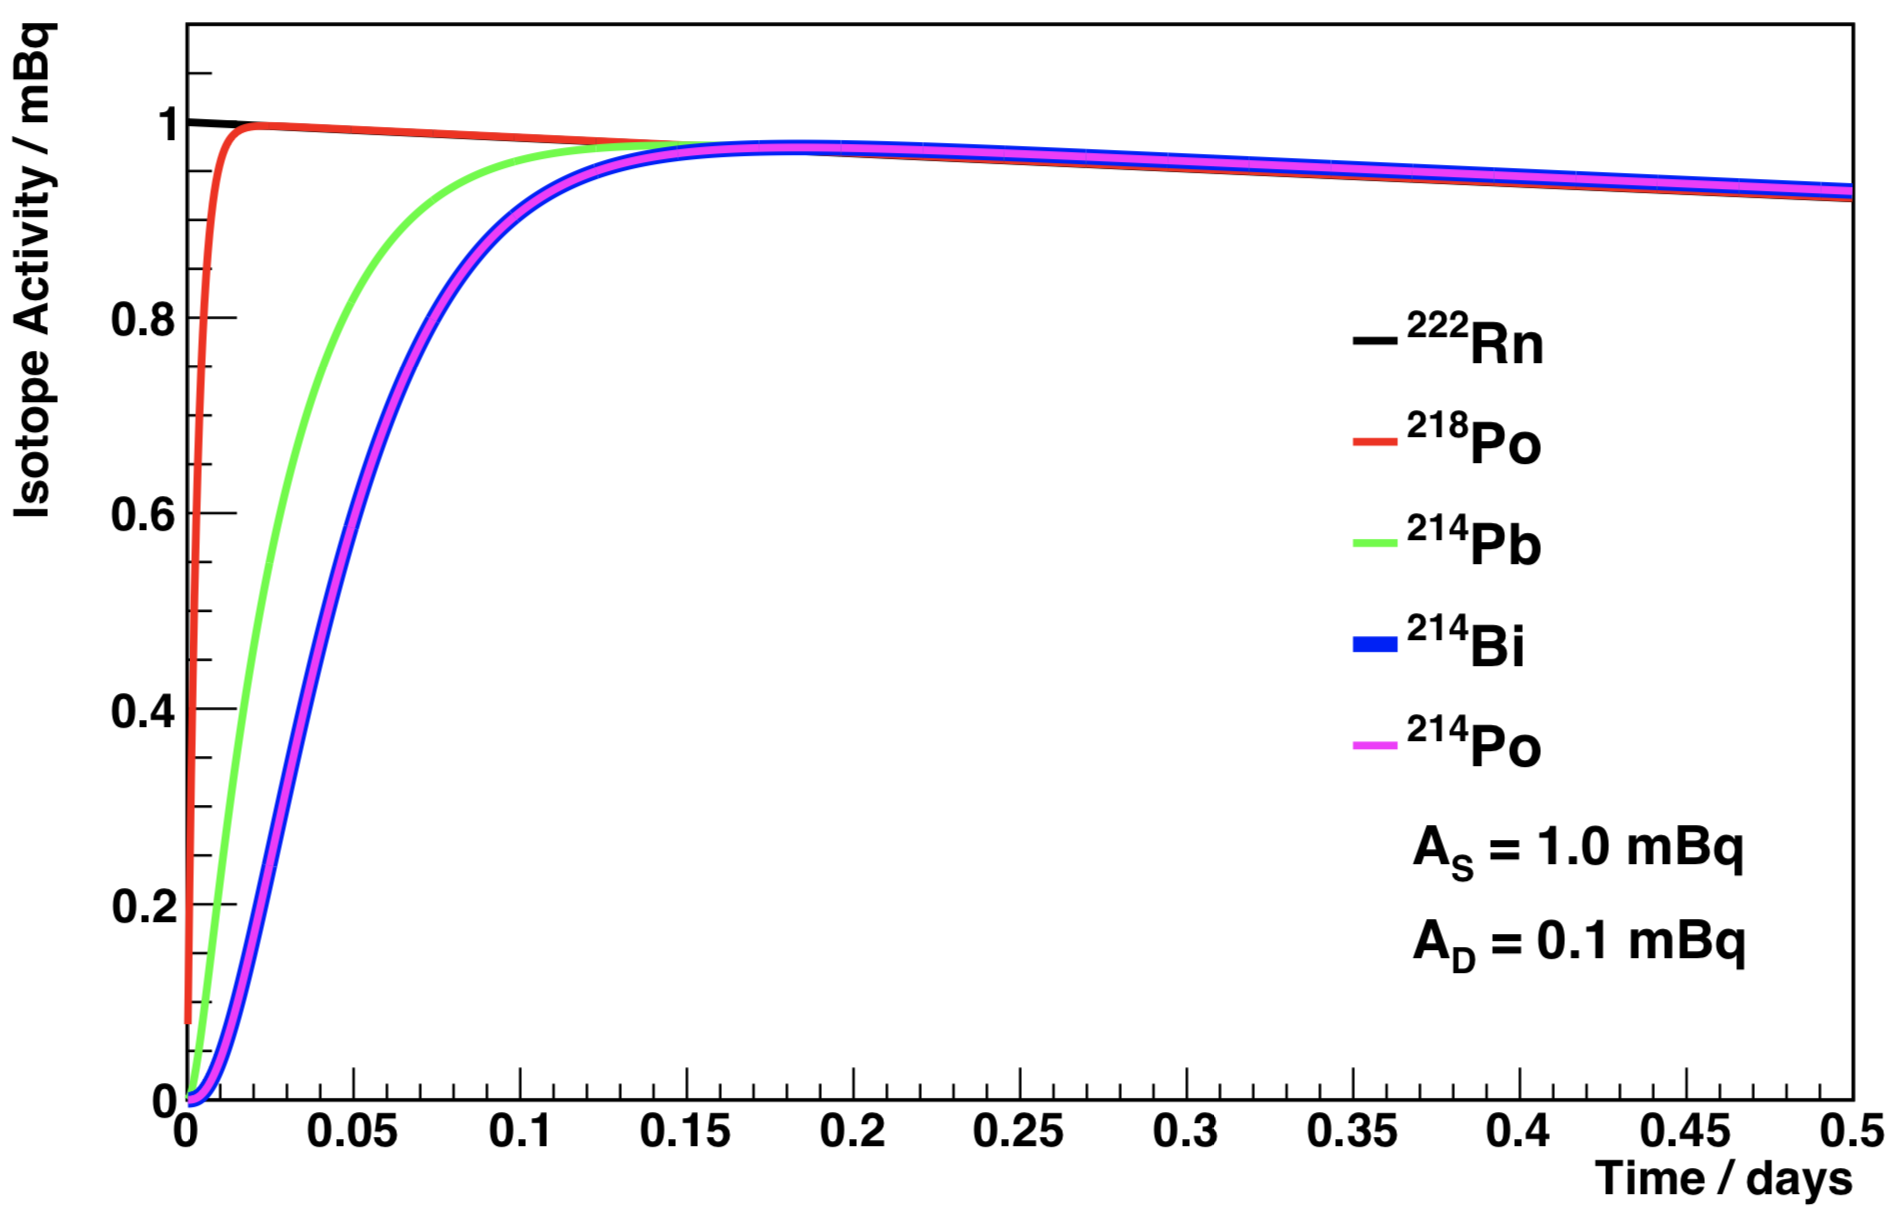
\includegraphics[scale=0.40]{Chapter_4/Figures/radon_chain_activities.png}
    \caption[The evolution of activities of the \RnTTT{} decay chain with respect to time under the starting condition of 1 mBq of \RnTTT{}.]
    {The evolution of activities of the \RnTTT{} decay chain with respect to time under the starting condition of 1 mBq of \RnTTT{}. $A_{D}$ represents the intrinsic background activity of the detector. Figure adapted from \cite{mott_2013}.}
    \label{fig:radon_chain_activity_evolution}
\end{figure}
%
Its important to note that the activity of \PoTOE{} quickly reaches an equilibrium with \RnTTT{}, whereas it takes $\sim4.5$ hours for \PoTOF{}. Hence, this slight delay needs to be taken into account if the emanation from a sample is transferred into the detector prior to equilibrium. Provided equilibrium is reached, the measured activity of both \PoTOE{} and \PoTOF{} will be equivalent to the activity of \RnTTT{}.


\newpage
\subsection{Electrostatic Detector}
\label{secsec:electrostatic_detector}

The electrostatic detector used in this work has been specifically developed for the use of ELEGANT V and Super-Kamiokande experiments in measuring low-levels of radon \cite{CHOI2001177, MITSUDA2003414}. A detector with identical specifications developed by the same group was later acquired for SuperNEMO for background studies, as detailed in \cite{mott_2013}. Its design capability can measure radon activities to 1-2 mBq/\cubicmeter{}, 2 orders of magnitude improvement upon commercially available radon detectors. The schematics of the system are shown in figure \ref{fig:elecrostatic_detector}. 
%
\begin{figure}[h!]
    \centering
    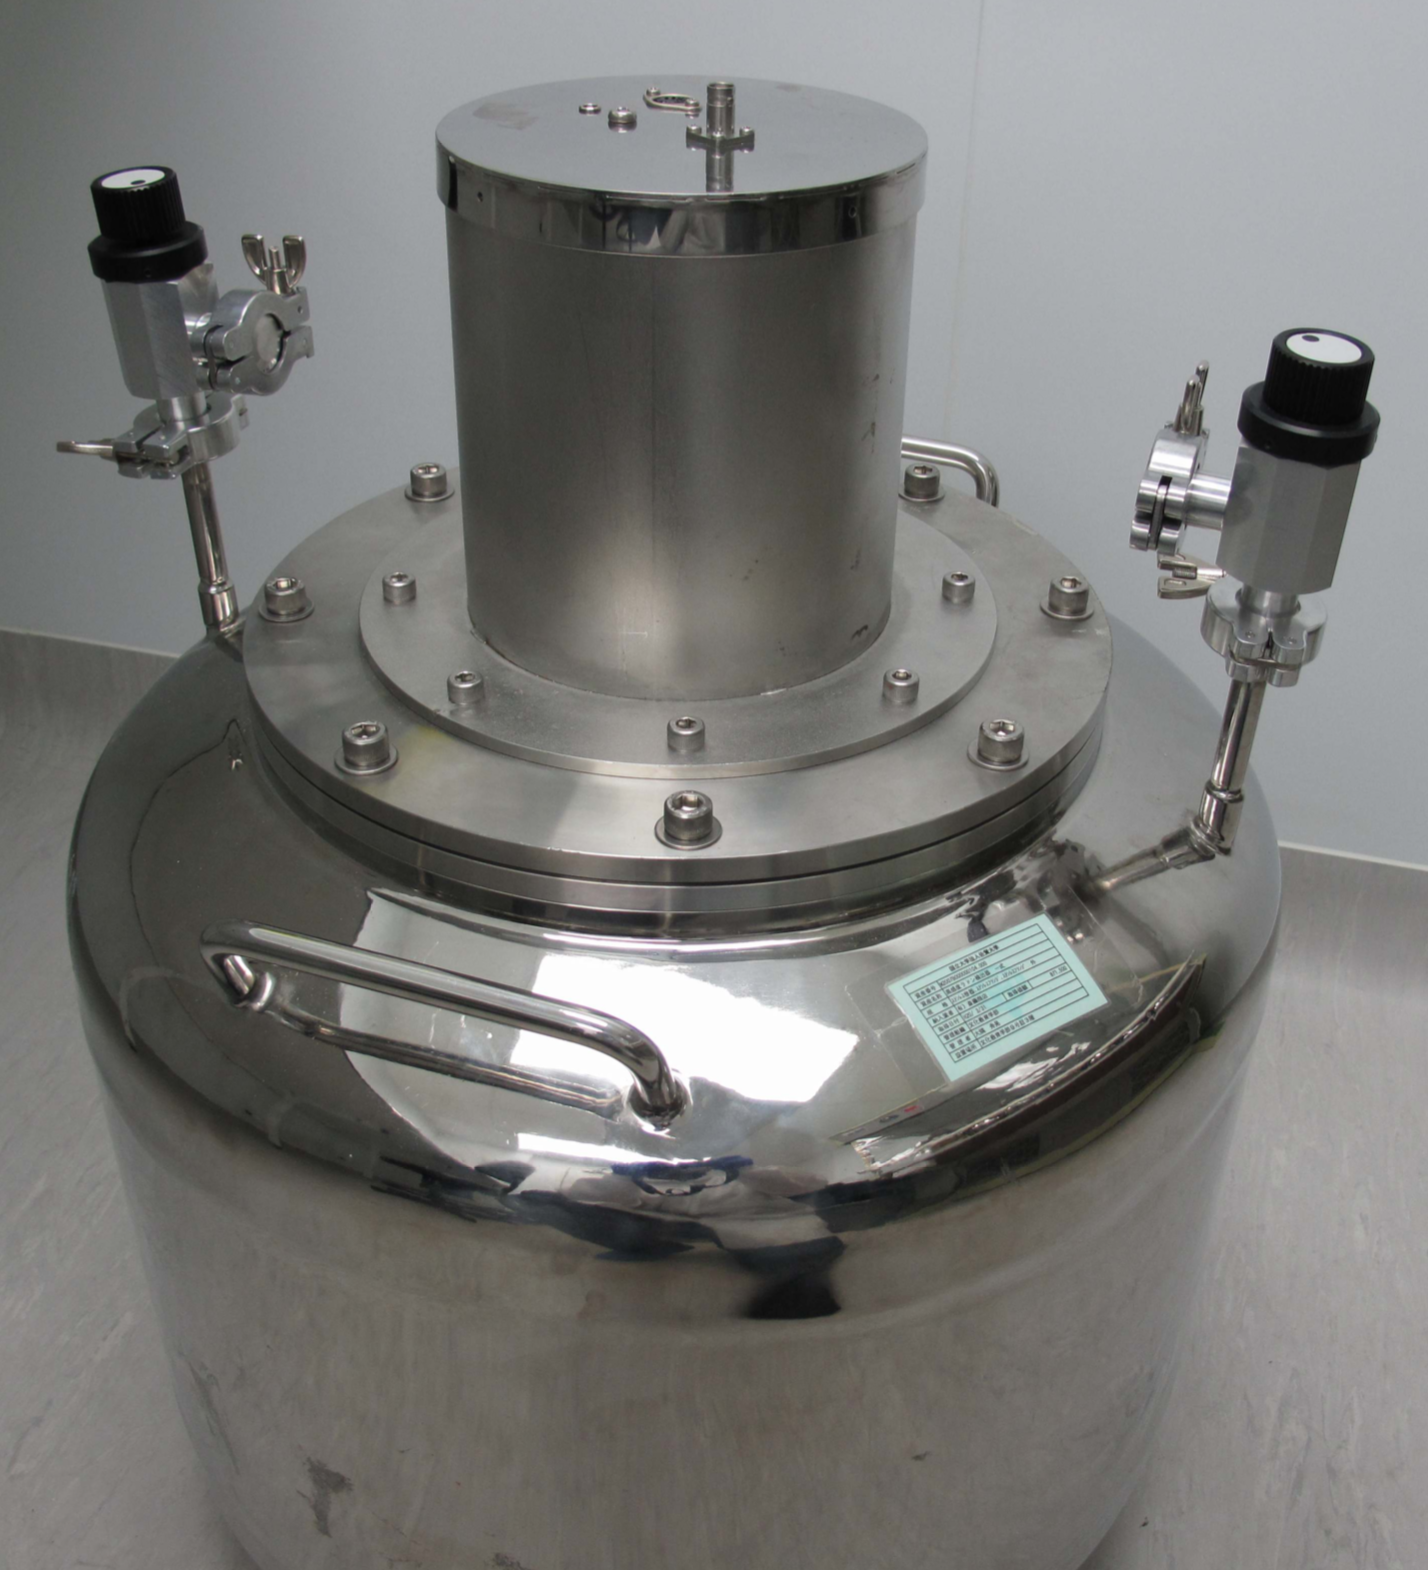
\includegraphics[scale=0.3]{Chapter_4/Figures/electrostatic_detector_1.png}
    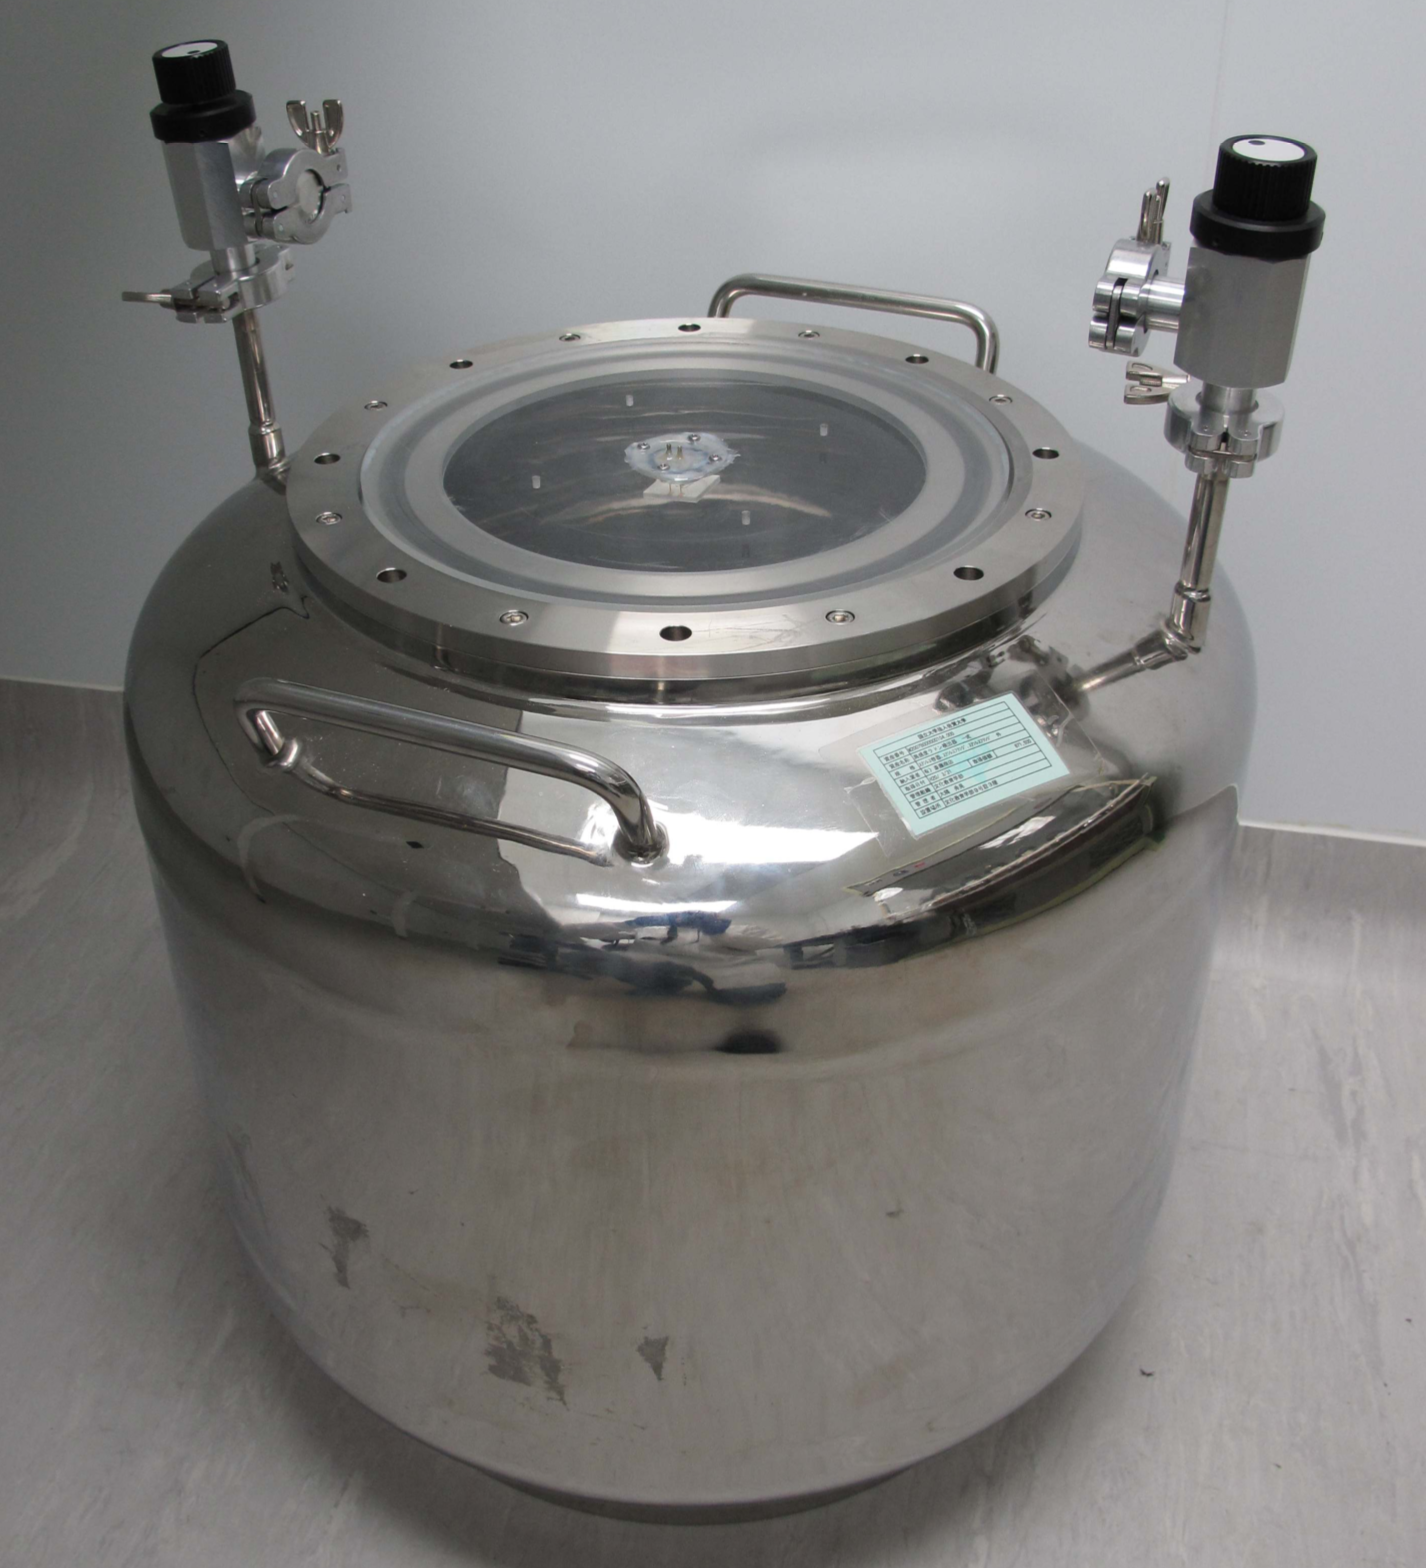
\includegraphics[scale=0.3]{Chapter_4/Figures/electrostatic_detector_2.png}
    \caption[Pictorial diagram of the electrostatic detector used for the radon emanation results published in this work.]
    {Pictorial diagram of the electrostatic detector used for the radon emanation results published in this work. Left shows the detector in full operational mode and the right shows it without its lid, where the feedthrough for the PIN-diode can be seen.}
    \label{fig:elecrostatic_detector}
    %----------
    \vspace{2cm}
    %----------
    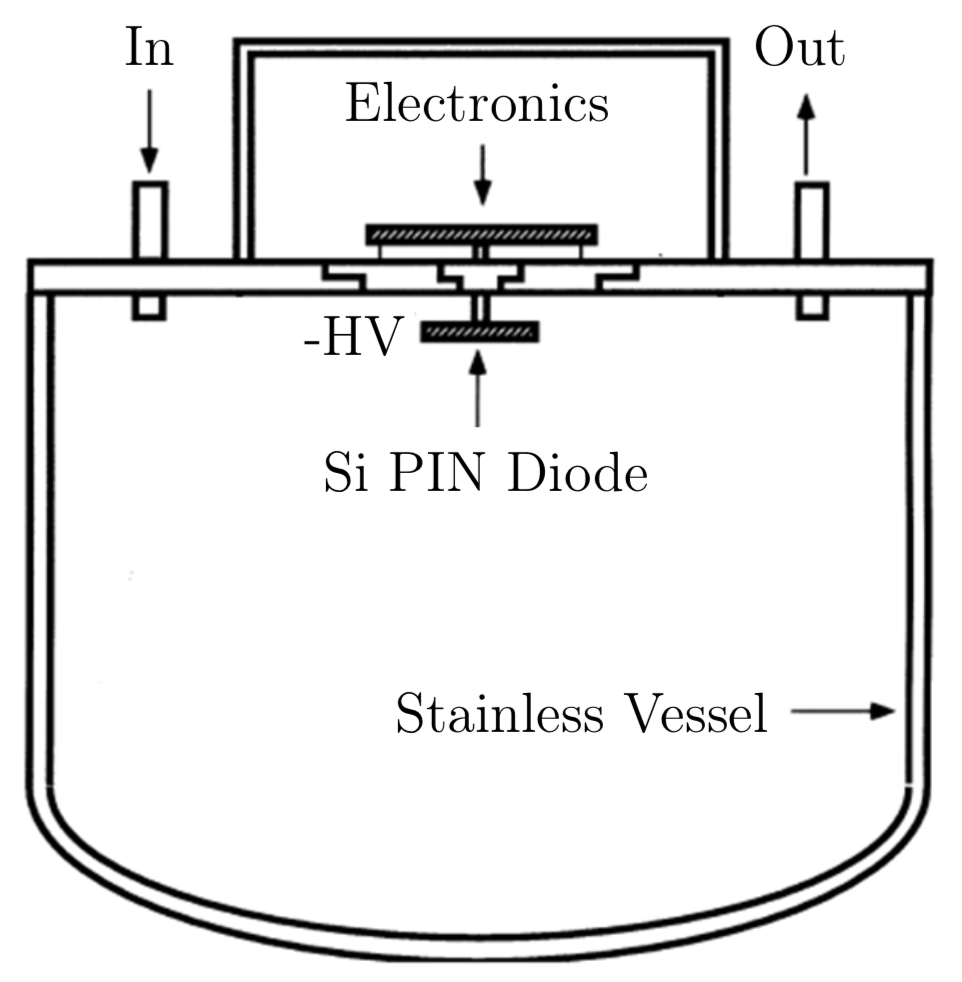
\includegraphics[scale=0.5]{Chapter_4/Figures/electrostatic_detector_schematic.png}
    \caption[A schematic diagram of the electrostatic detailing the electronics.]
    {A schematic diagram of the electrostatic detailing the electronics.}
    \label{fig:elecrostatic_detector_schematic}
\end{figure}
%

The simple design of the detector consists of an electro-polished stainless steel chamber with a 70 litre volume with a silicon PIN-diode attached to the top of the detector as shown schematically in figure \ref{fig:elecrostatic_detector_schematic}. The associated detector electronics are housed in the lid of the detector, separated from the measurement chamber by a sheet of perspex with a feedthrough for the PIN-diode. The detector has an inlet and an outlet valve for gas flow, all either metallic or have been coated with styrene butadiene rubber (SBR) to reduce the internal radon background that diffuse out or through material and into the detector volume. An electric field is generated inside the chamber by applying a negative high voltage (typically −1500 V) onto the PIN-diode.
 
In a standard operation, a sample is usually left to emanate for a set amount of time after which the gas content is transferred into the detection volume. The radon atoms decay within the volume result in daughter nuclei that are predominantly positively charged ions (\SI{87.3\pm1.6}{\percent} \cite{PAGELKOPF20031057}). These ions are effectively collected by the PIN-diode as a result of the applied electric field. The \alpha{} particles emitted from the \potoe{} and \potof{} ions are detected by the PIN-diode as they undergo \alpha{}-decay and are distinguished by the energies they deposit; \SI{6.1}{\mega\electronvolt} and \SI{7.9}{\mega\electronvolt}, respectively. 


\subsection{Detector Efficiency}
\label{sec:detector_efficiency}

Understanding the response of the detector to a known activity of radon is vital in modelling the detector response and correcting the measured activity for detector related efficiencies. In modelling this, a calibration source of \RaTTS{} (Pylon Electronics, RN-1025) with a known activity of 1.32 kBq was used. The source is designed to allow for gas flow through the material to transfer the emanated radon effectively into the detector volume, ensuring all of the radon to be exhausted.

The method used in calibrating the detector is sometimes referred to as the \textit{spike} method. The source volume is initially flushed out by the use of a helium carrier gas by around 10--100 times the volume of the source to ensure all of the radon is exhausted thoroughly. The volume is then sealed for a set amount of time to allow for a set amount of radon to build up. In a typical calibration, helium is used as a carrier gas to move 2.5 Bq of radon into the detector. The background spectrum of the electrostatic detector without and with a typical calibration source injection is shown in figure \ref{fig:background_calibration_spectrum}. 
%
\begin{figure}[hb!]
    \centering
    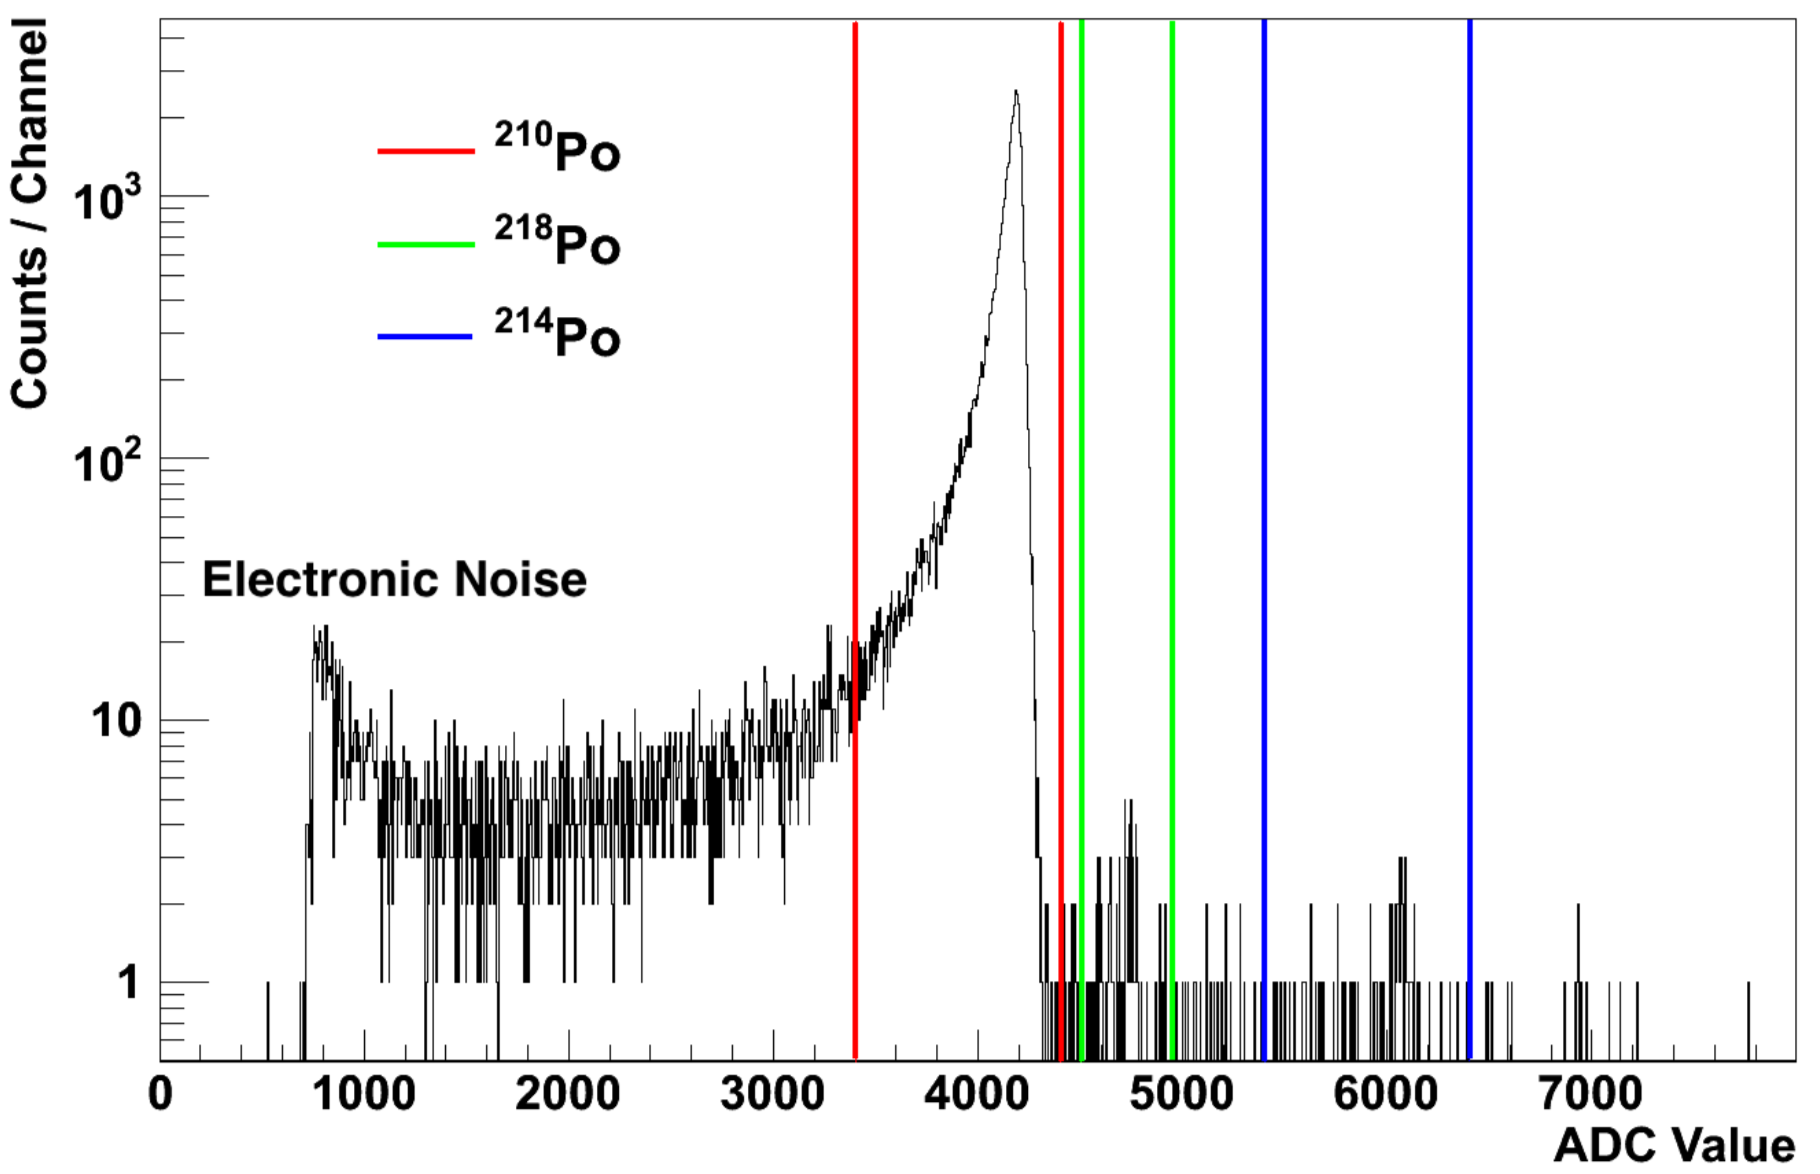
\includegraphics[scale=0.23]{Chapter_4/Figures/background_spectra.png}
    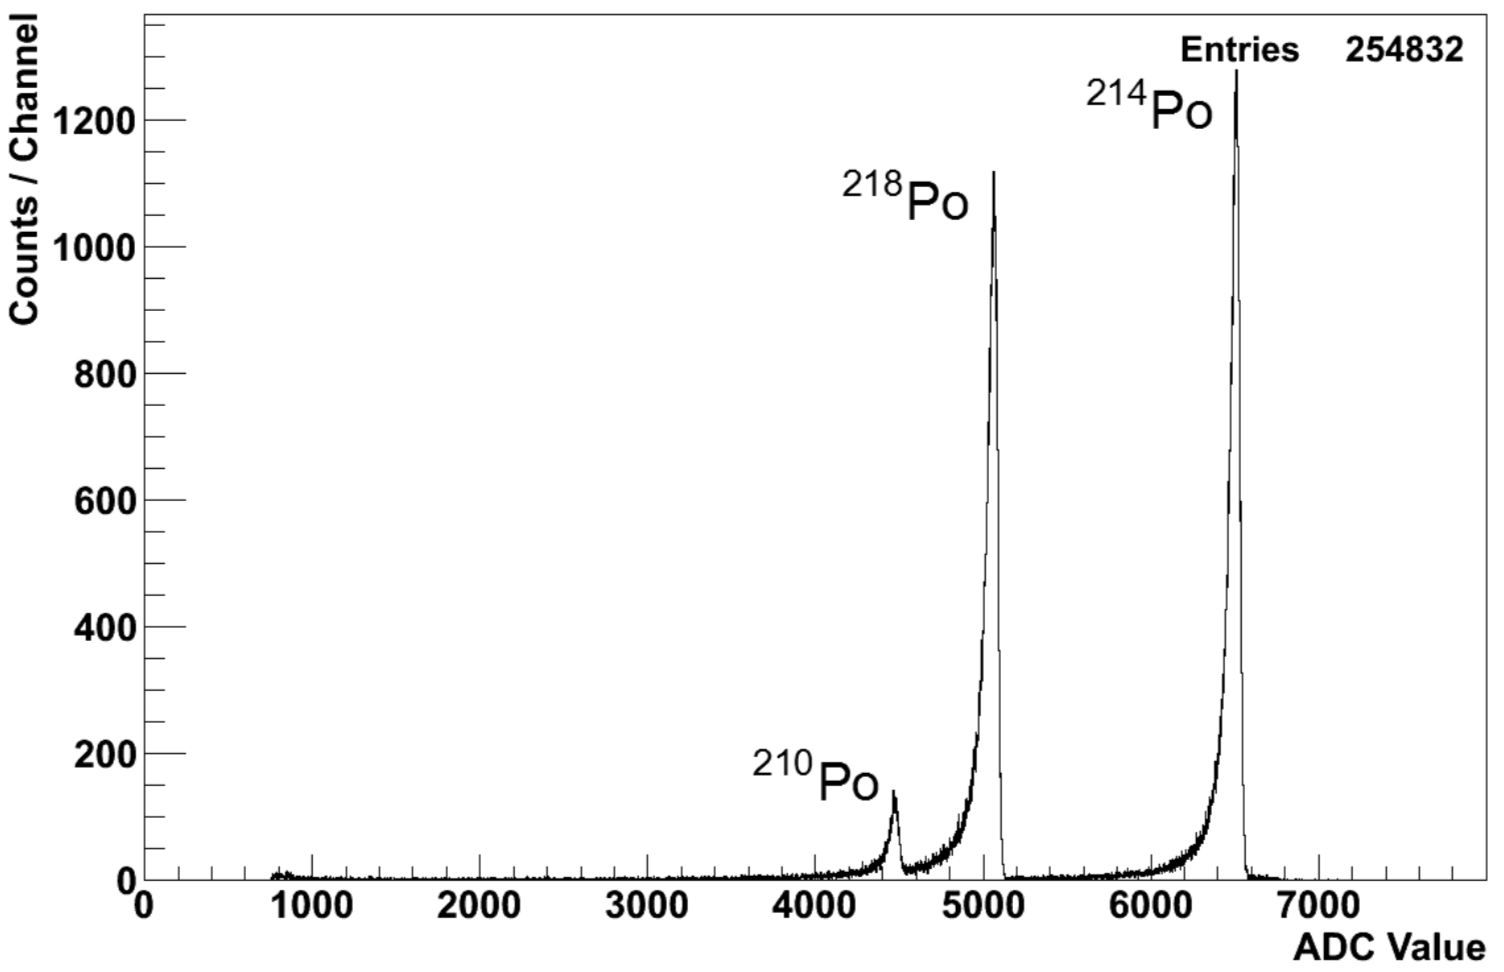
\includegraphics[scale=0.28]{Chapter_4/Figures/calibration_spectra.png}
    \caption[Spectrum from the electrostatic detector without and with 2.5 Bq of the calibration present.]
    {Spectrum from the electrostatic detector without (left) and with (right) 2.5 Bq of the calibration source present. The spectral peaks of \PoTOZ{}, \PoTOE{} and \PoTOF{} are displayed from left to right. The red, green and blue windows are used to select regions of the spectrum associated with the isotopes of interest for further analysis.}
    \label{fig:background_calibration_spectrum}
\end{figure}
%

In an event where the ionised radon progeny attaches onto the PIN-diode and undergoes \alpha{}-decay, the kinetic energy carried by the \alpha{}-particle can be identified by the induced amplitude of the signal. The energy resolution of these detectors is such that the peaks observed for the three isotopes of polonium are clearly visible after the source injection. Although some \PoTOZ{} is present as a result of the calibration source, the majority of its observed activity is as a result of residual exposure of the PIN-diode and its longer half-life of $\sim140$ days. This residual activity is more apparent on the background spectrum of the detector prior to source injection, as seen on the left in figure \ref{fig:background_calibration_spectrum}. Although one may naively think that the peaks of \PoTOE{} and \PoTOF{} should be identical in activity (counts), this is often not the case. An explanation for this apparent difference in efficiency could be resulting from \PoTOF{} decay taking place after multiple intermediate isotopic decays. The intermediate isotopes \PbTOF{} and \BiTOE{} are assumed to be predominantly created as ions and as a result are collected by the PIN-diode. This results in more \PbTOF{} either on the PIN-diode or close to the PIN-diode, reducing the probability of neutralisation, which often takes place under trace amounts of impurities, such as nitrous oxide (N$_{2}$O). Although \alpha{}-decay counts from both \PoTOE{} and \PoTOF{} can be used to reconstruct the radon activity, the activities quoted are from \PoTOF{} due to its higher detection efficiency. Furthermore, despite the energy resolution, some overlap between the \PoTOE{} and \PoTOZ{} peaks are unavoidable.
%
\begin{figure}[b!]
    \centering
    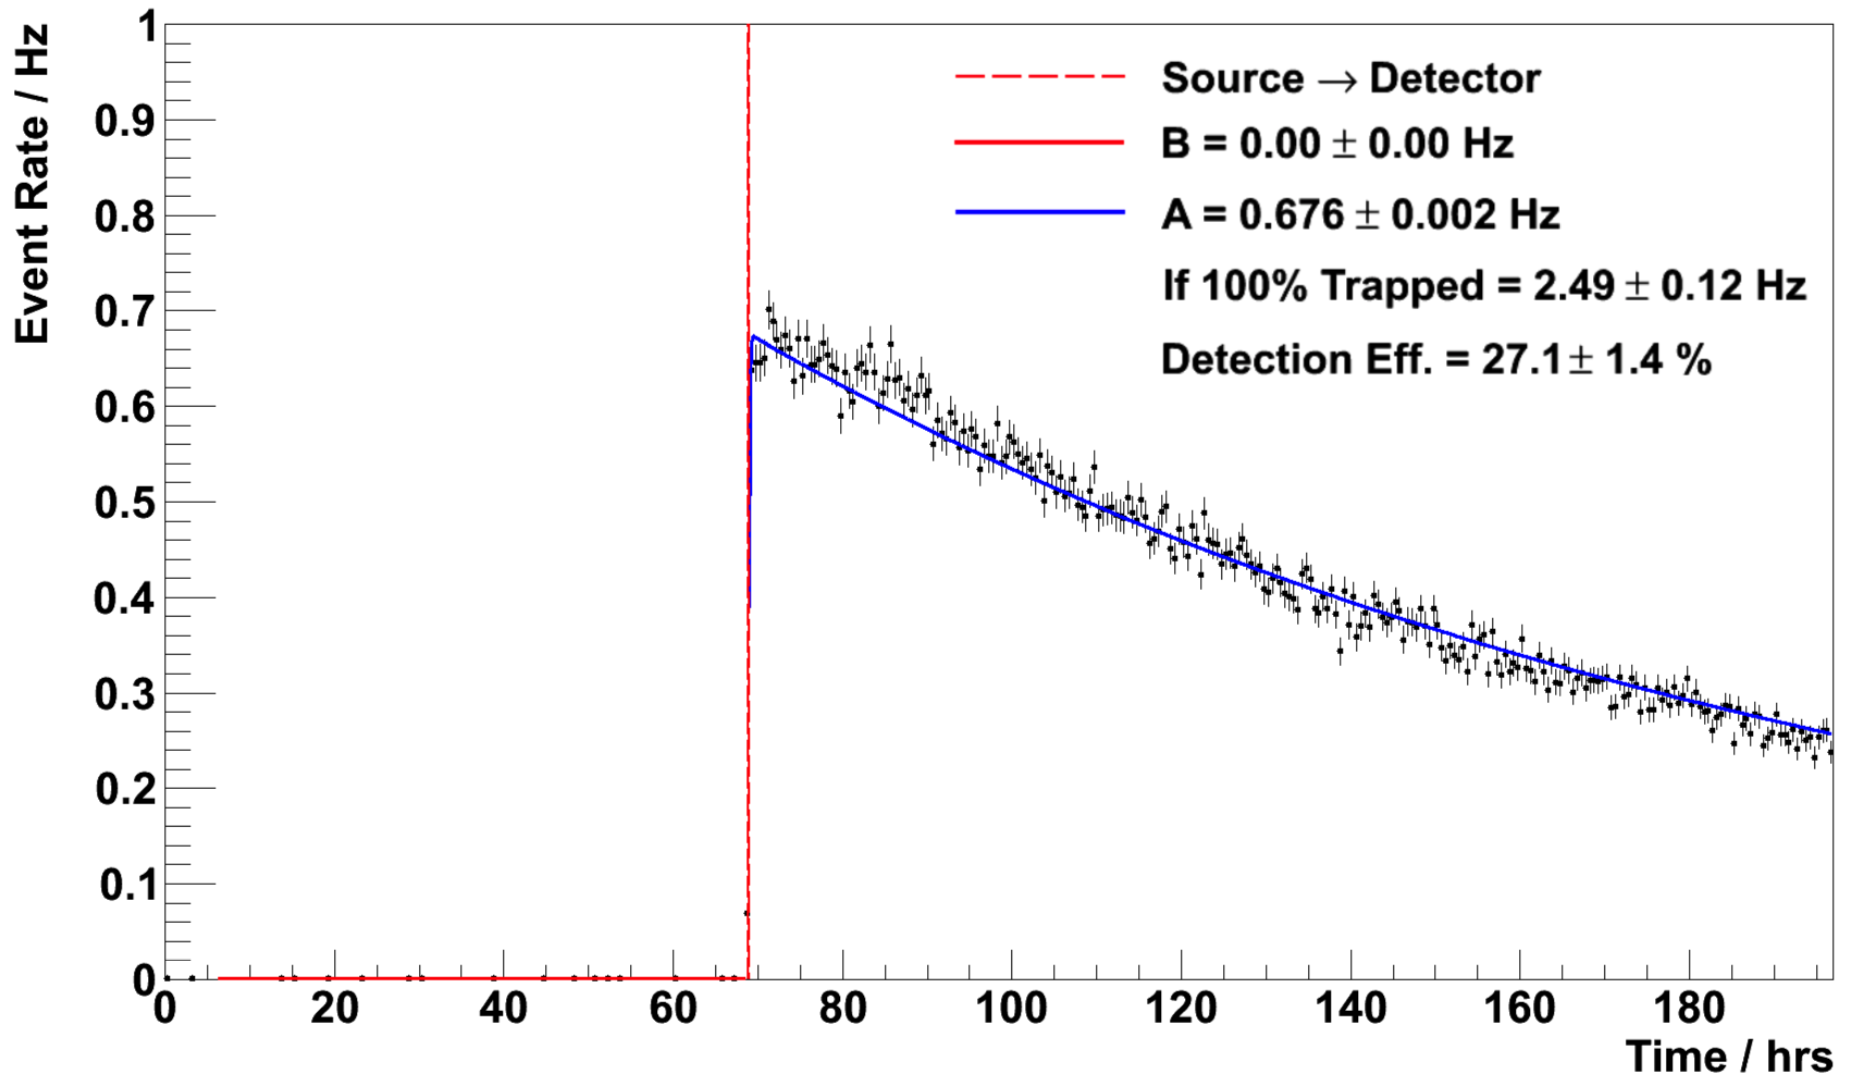
\includegraphics[scale=0.23]{Chapter_4/Figures/Po_218_Calibration.png}
    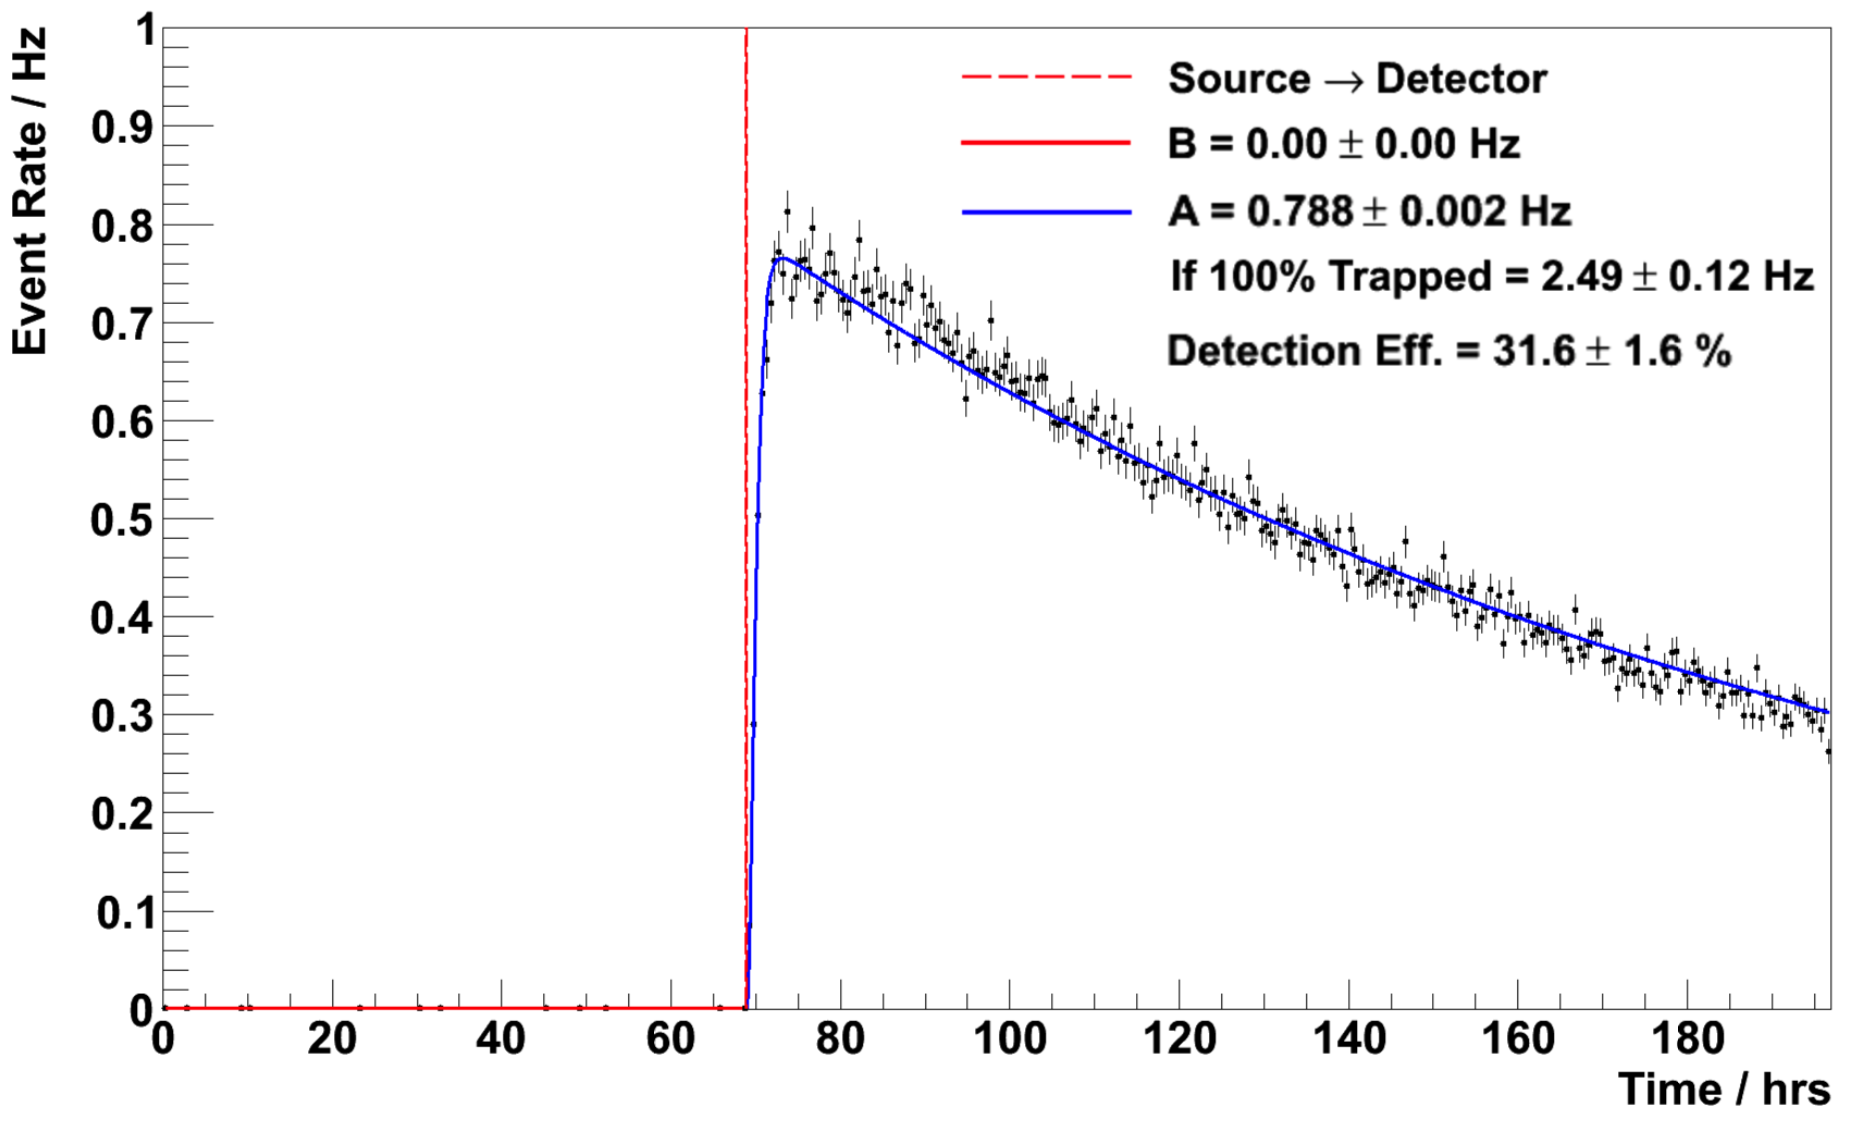
\includegraphics[scale=0.23]{Chapter_4/Figures/Po_214_Calibration.png}
    \caption[\PoTOE{} and \PoTOF{} event rates for a calibration injection of 2.5 Bq of radon into the detector via a helium carrier gas.]
    {\PoTOE{} (left) and \PoTOF{} (right) event rates for a calibration injection of 2.5 Bq of radon into the detector via a helium carrier gas. The fitted black line shows the expected response for the given isotope with all half-lives fixed to their known values.}
    \label{fig:calibration_decay_fit}
\end{figure}
%

To calculate the detection efficiency, the peaks of \PoTOE{} and \PoTOF{} are initially selected with predetermined windows, and their respective activities are fit using decay equations derived from equation \ref{eq:isotopic_chance_in_chain} and shown in detail in \cite{mott_2013}. A typical result from a 2.5 Bq of radon injection into the detector is shown in figure \ref{fig:calibration_decay_fit}. The detection efficiency was then calculated as $27.1\pm1.4\%$ and $31.6\pm1.6\%$ for \PoTOE{} and \PoTOF{}, respectively. The associated errors are dominated by the uncertainties on the source activity. Its important to note that the maximum detection efficiency achievable using this technique is 50\%, as half of the \alpha{}-particles are emitted away from the PIN-diode and hence never measured. 


\subsection{Detector Background Measurements}
\label{secsec:concentration_line}


\subsubsection{Detector Background}

The sensitivity of the detector and the measured activities are not limited to the efficiency of the detector alone but also the detector background rate. In general, a typical measurement would include a measurement of the background rate of the detector $\sim5$ days prior to the transfer. This background rate is then subtracted from the measured activity post transfer. Additionally, much longer background measurements are performed periodically to ensure the stability of the detector. In such measurements, the detector is fully sealed to both the gas line and the environment and the radon activity is continuously measured. The energy spectrum from this type of run is different to that of a calibration run as can be seen in figure \ref{fig:detector_background_spectrum}.
%
\begin{figure}[b!]
    \centering
    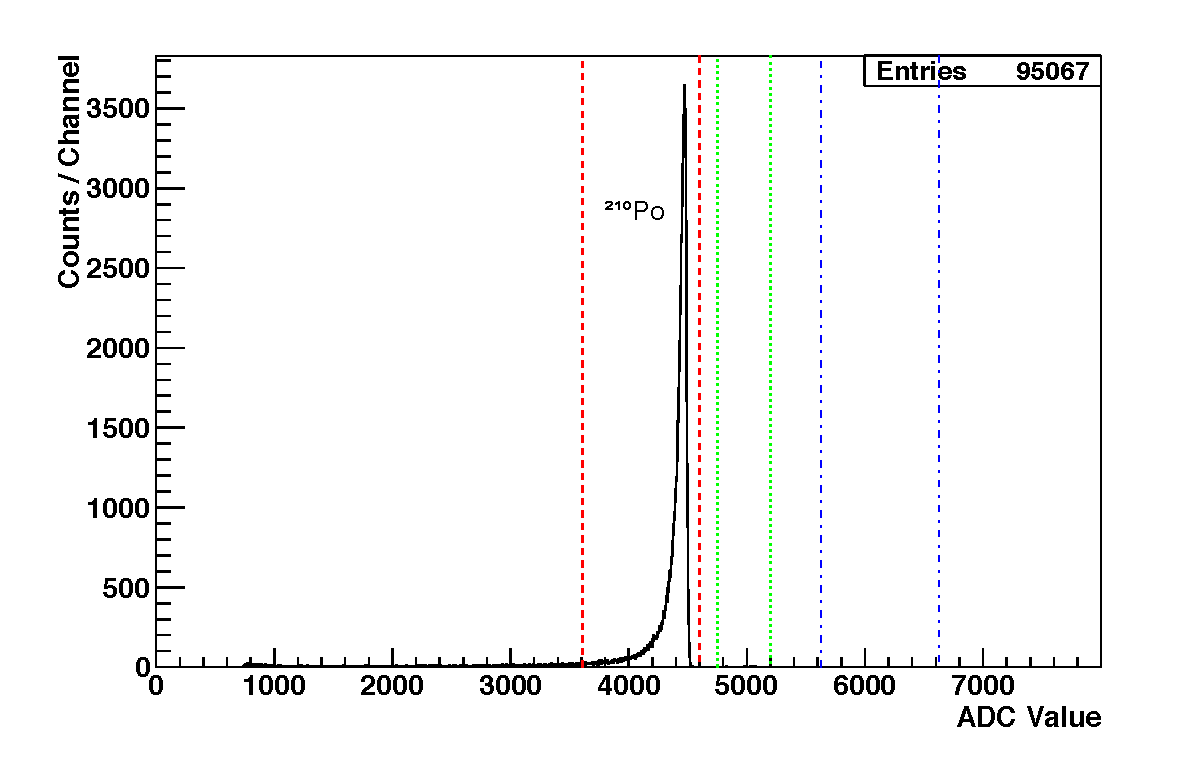
\includegraphics[scale=0.43]{Chapter_4/Figures/det_background/Spectrum_det_background.pdf}
    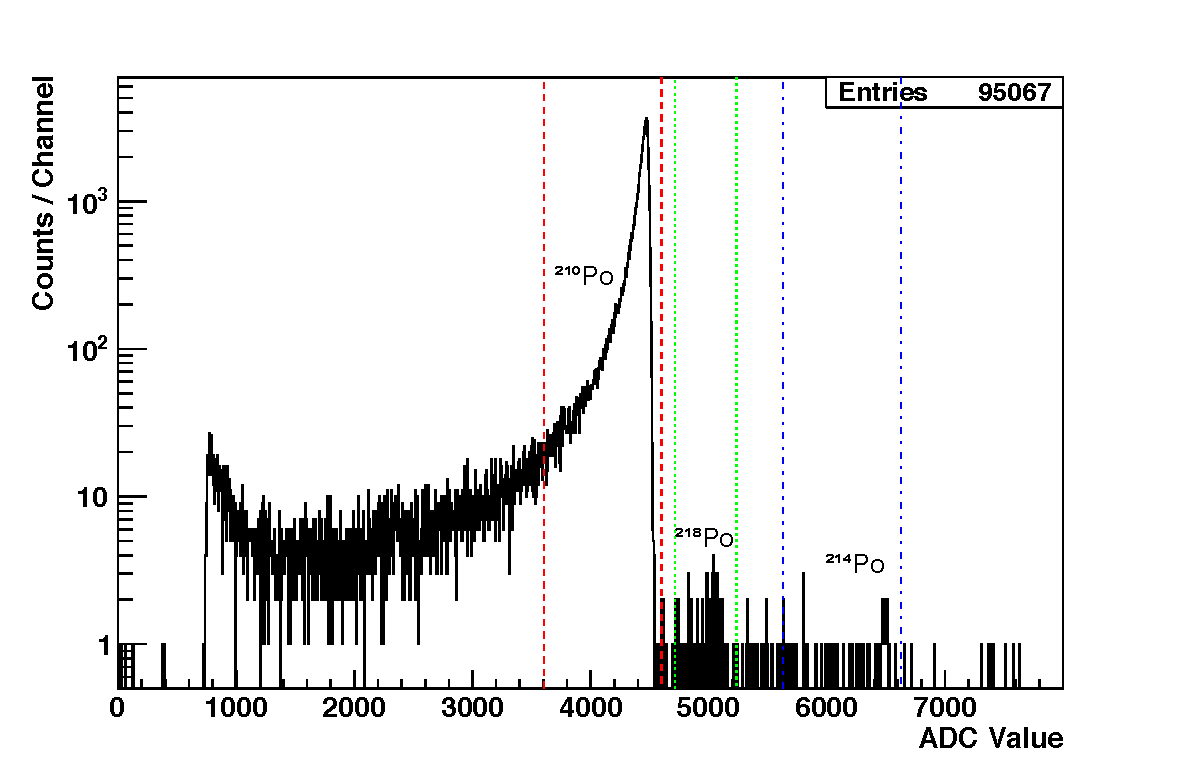
\includegraphics[scale=0.43]{Chapter_4/Figures/det_background/LogSpectrum_det_background.pdf}
    \caption[Energy spectrum of a long radon emanation detector backgrounds showing the peaks of \PoTOZ{}, \PoTOE{} and \PoTOF{}.]
    {Energy spectrum of a long detector background measurement with linear and logged y-axis. The peaks of \PoTOZ{}, \PoTOE{} and \PoTOF{} are displayed accordingly.}
    \label{fig:detector_background_spectrum}
\end{figure}
%

The observed spectrum is similar to that of a typical material measurement with a dominant \PoTOZ{} that has accumulated onto the PIN-diode from prior calibration runs. The peaks are selected with pre-determined windows as shown by the vertical lines on figure \ref{fig:detector_background_spectrum} and the activity of \PoTOF{}, along with that of \PoTOZ{} is shown in figure \ref{fig:detector_background_rates}. 
%
\begin{figure}[t!]
    \centering
    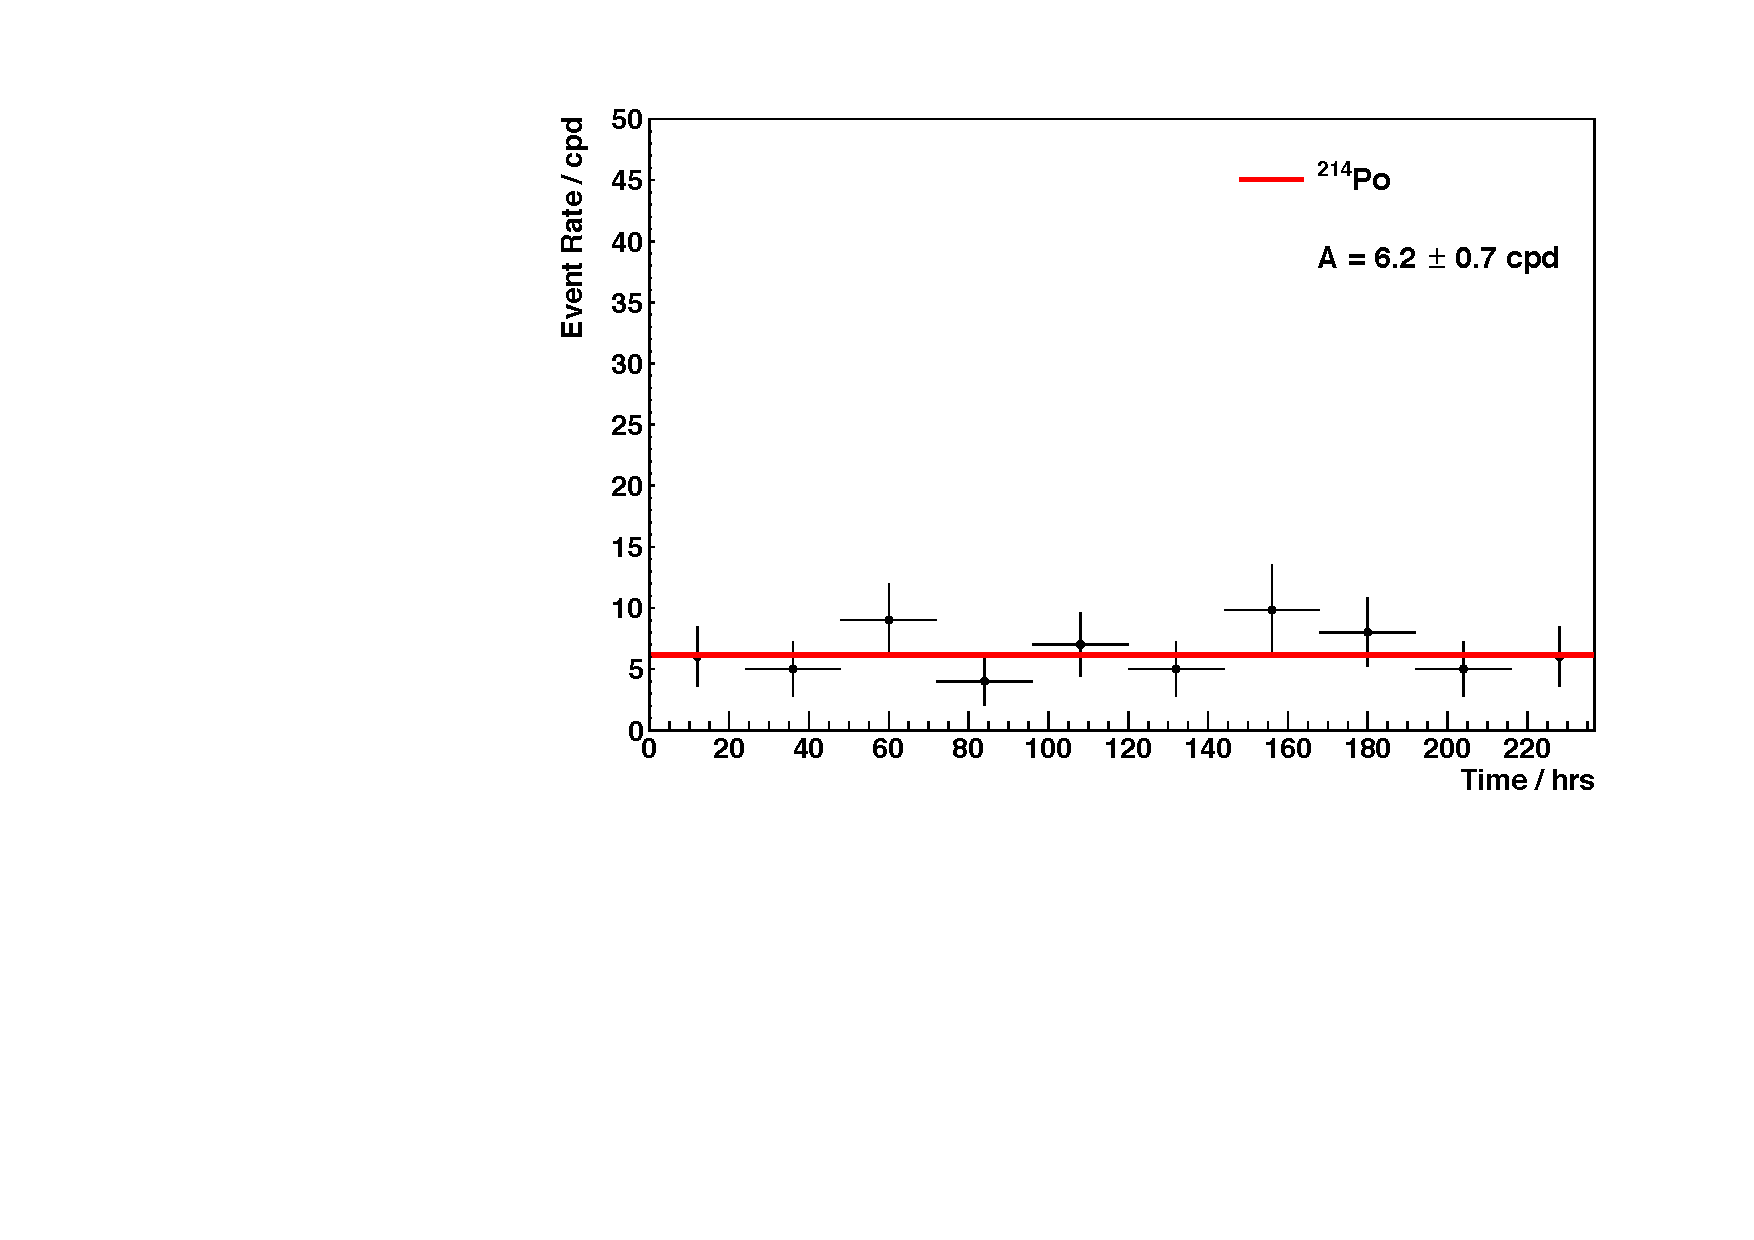
\includegraphics[scale=0.43]{Chapter_4/Figures/det_background/Po214_det_background.pdf}
    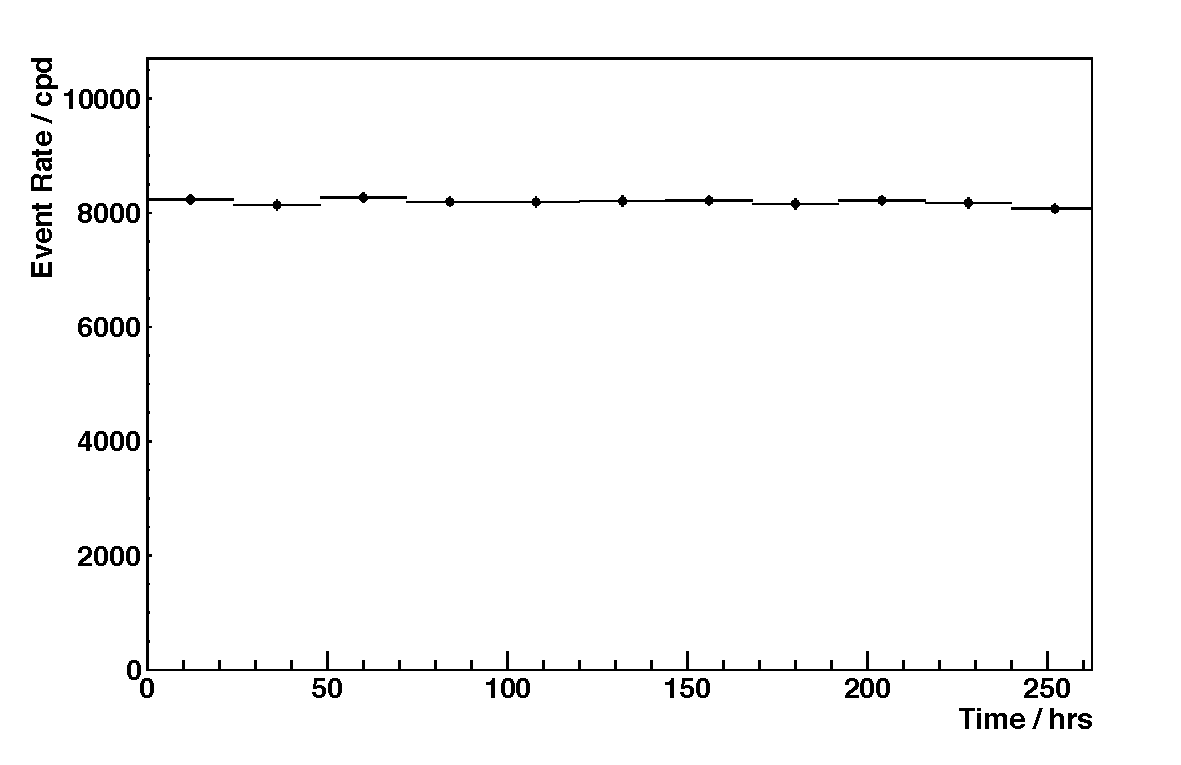
\includegraphics[scale=0.43]{Chapter_4/Figures/det_background/Po210_det_background.pdf}
    \caption[\PoTOF{} and \PoTOZ{} event rates for a typical background measurement run.]
    {\PoTOF{} (left) and \PoTOZ{} (right) event rates for a typical background measurement run. The \PoTOF{} rate shows a relatively low background level, whereas the \PoTOZ{} shows the stability of the detector.}
    \label{fig:detector_background_rates}
\end{figure}
%

The inferred \PoTOF{} rate, which is the primary channel to reconstruct the radon emanation rate shows an averaged daily rate of $6.2\pm{}0.7$\,counts-per-day (cpd). The detector in this measurement is initially flushed thoroughly and filled with helium gas, so by using the detector efficiency of 31.6\% for \PoTOF{}, the intrinsic activity of the detector is determined to be $0.20\pm0.02$\,mBq. Besides the \PoTOF{} rate, the \PoTOZ{} rate is also measured as shown in figure \ref{fig:detector_background_rates}. Although this does not inform on the radon activity, it is a useful measure in checking the stability of the detector and the DAQ over time, as this rate is expected to be constant over a measurement period. 

\subsubsection{Emanation Chamber Background}

In conducting measurements on samples, the radon emanated from these samples are initially collected in the emanation chambers as previously mentioned. Although these chambers are made from stainless steel, to fully account for all potential backgrounds, the chamber background used for the LZ was determined by a blank measurement. The chamber cleaned and enclosed for 30 days, after which the contents were flushed into the detector for a measurement. Both the \PoTOE{} and the \PoTOF{} spectra agreed with a detector background-only scenario, hence an upper limit was placed on the chamber background. Details of this measurement can be found in \cite{xin_2017}. The 90\% CL activity placed on \PoTOE{} and \PoTOF{} were $< 0.246$ mBq and $< 0.187$ mBq, respectively.


\subsection{System Design and Schematics}
\label{secsec:system_design_schematics}

The electrostatic detector as detailed in the previous sections is part of a large system that handles gas flow in and out of the sample chamber and detector. A pictorial and a schematic diagram of the design is shown in figures \ref{fig:detector_design_picture} \& \ref{fig:detector_design_schematic}.
%
\begin{figure}[]
    \centering
    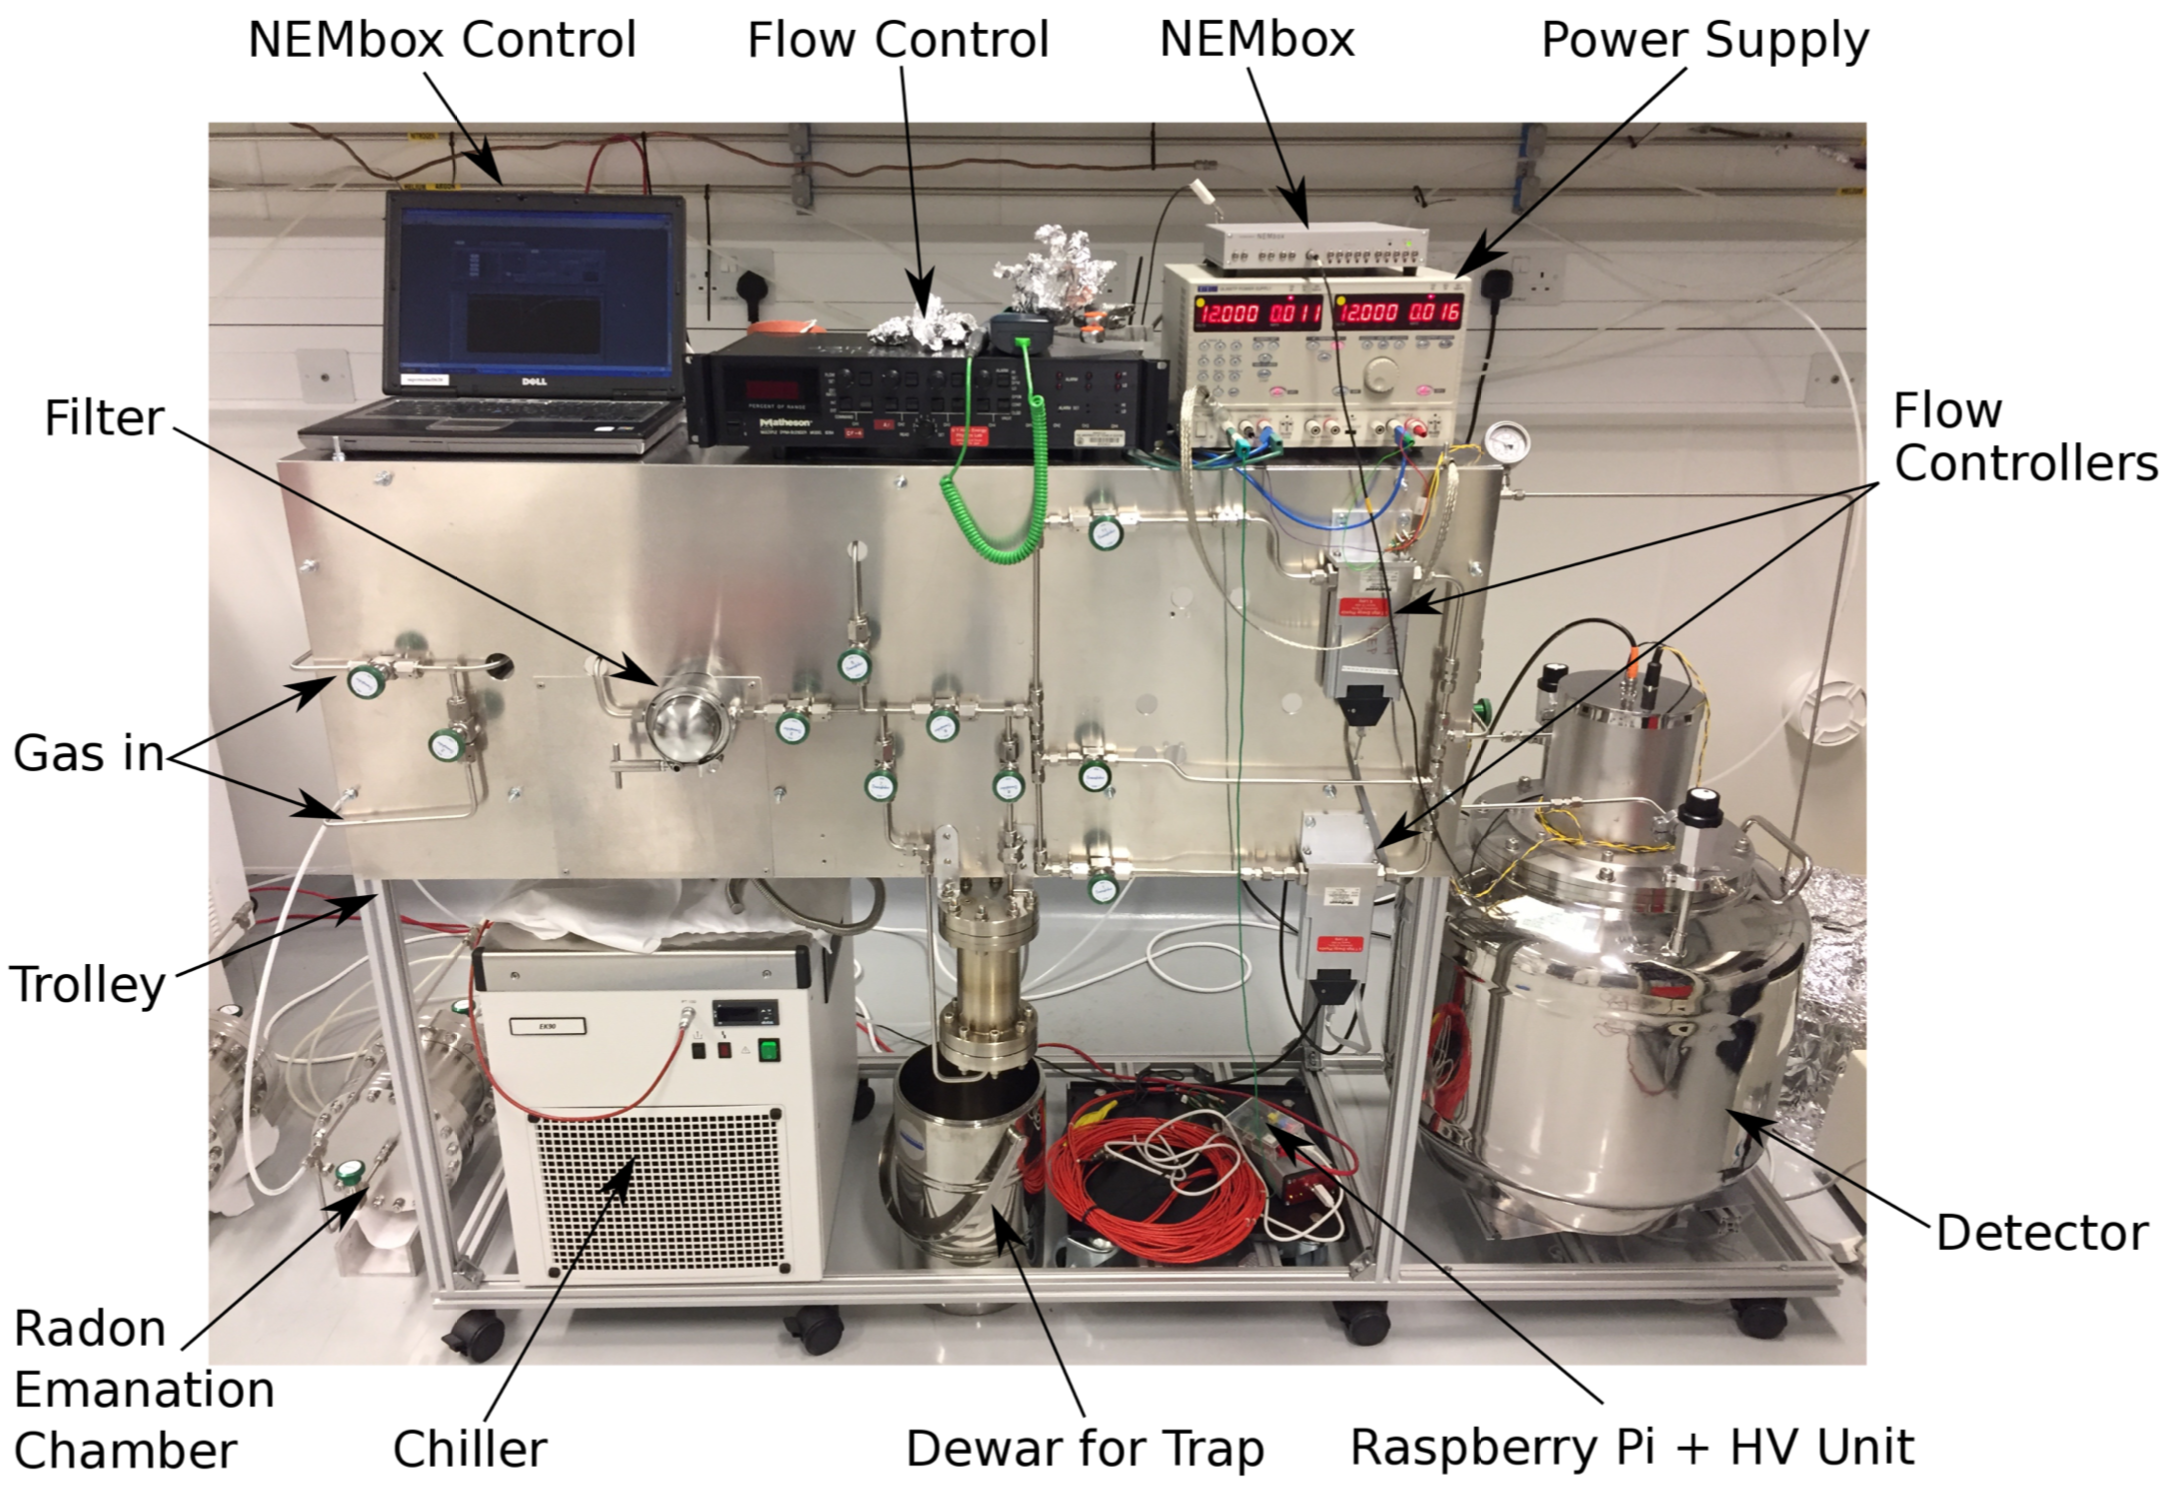
\includegraphics[scale=0.4]{Chapter_4/Figures/radon_system_design.png}
    \caption[A pictorial diagram of the UCL radon emanation system with key components highlighted.]
    {A pictorial diagram of the UCL radon emanation system with key components highlighted.}
    \label{fig:detector_design_picture}
\end{figure}
%
%
\begin{figure}[]
    \centering
    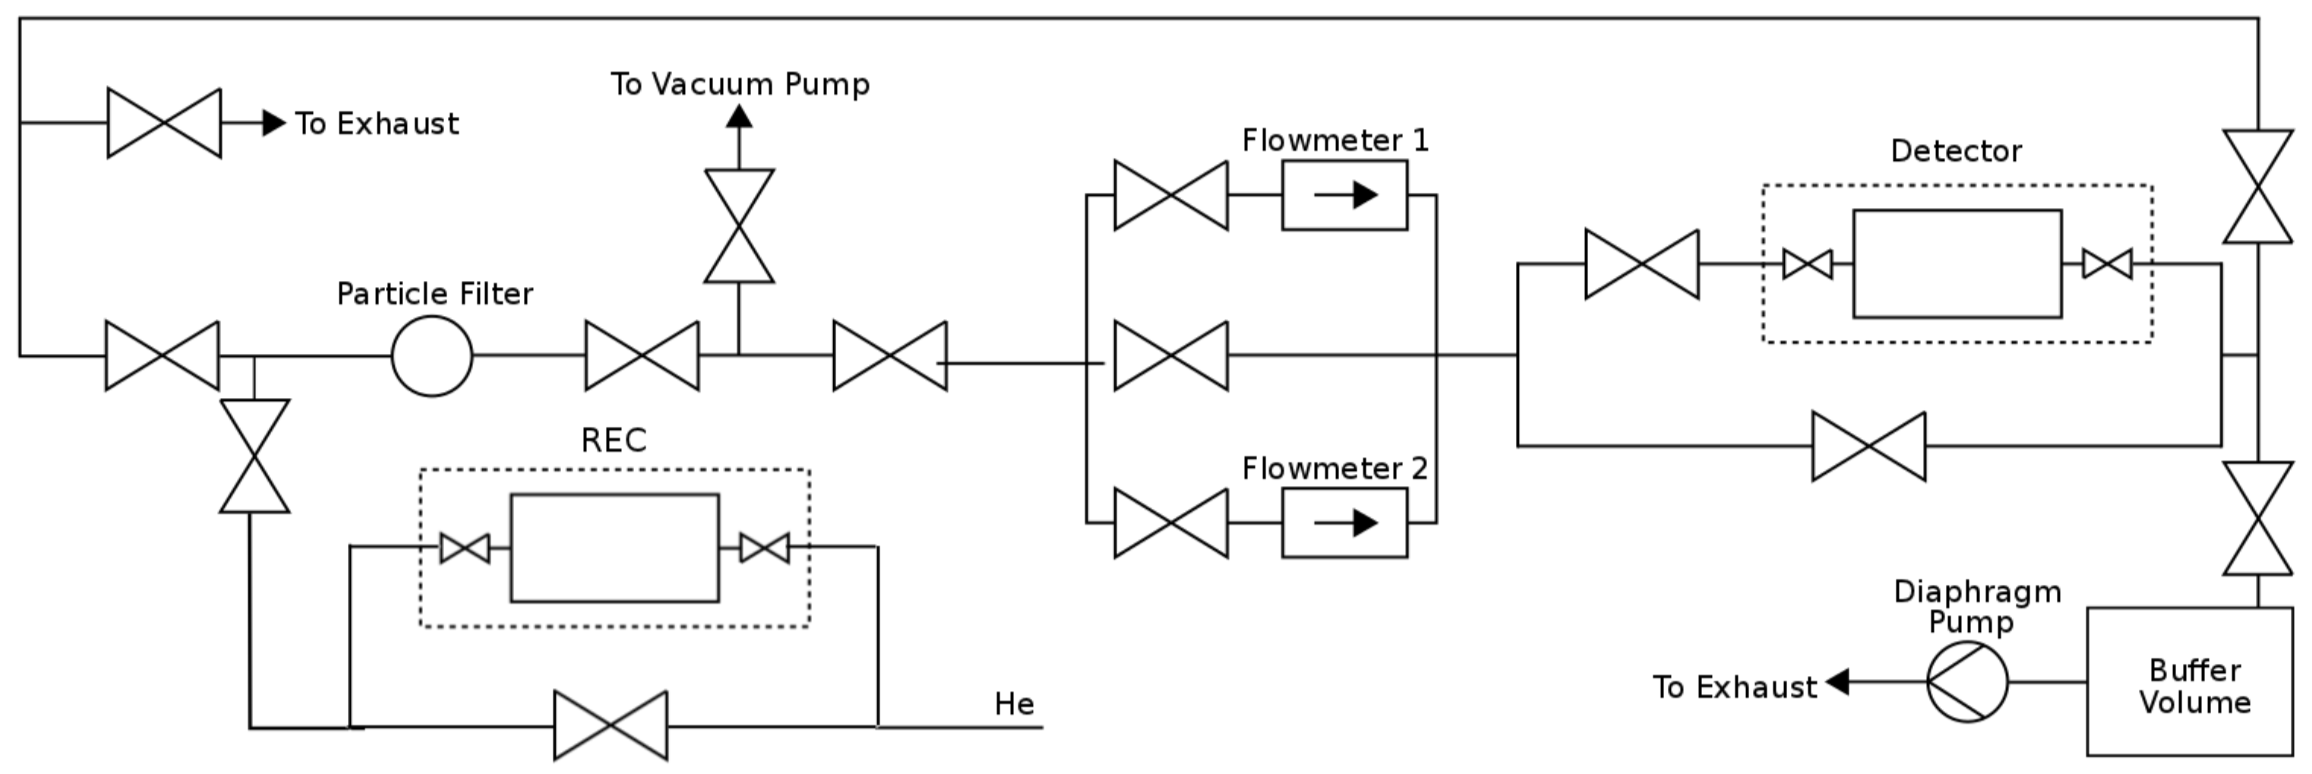
\includegraphics[scale=0.38]{Chapter_4/Figures/radon_system_pid.png}
    \caption[A schematic diagram of the UCL radon emanation system.]
    {A schematic diagram of the UCL radon emanation system.}
    \label{fig:detector_design_schematic}
\end{figure}
%

The system is design to facilitate a high degree of flexibility in operation. The carrier gas enters from the location marked as \textit{He} and can either flow through the radon emanation chamber (REC) or by-pass the chamber; crucial for calibration source injection or flushing the system without impacting the source emanation with the REC. Although helium has been used as the primary gas carrier, nitrogen can also be injected through the same flow path. Prior to entry, the gas is initially passed through an activated charcoal trap stored in an ultra-low temperate freezer (193 K) with 0.5 micron stainless steel particulate filters fitted on both ends to reduce particulate contamination. The charcoal trap scrubs the radon generated from the cylinders of the gas carriers to supply radon-free gas into the entire system. The carrier gas is then directed by a series of valves, with a flow meter determining the flow rate. All pipework is made from stainless steel and all valves are fully metallic, which reduces radon emanation.

The system operates two 2.7 L stainless steel chambers as the emanation media, as shown pictorially in figure \ref{fig:detector_chamber}. Once the sample is sealed inside the chamber, the chamber is flushed thoroughly to remove any ambient radon trapped inside and checked for leaks using a helium leak detector (GasCheck Tesla Helium Leak Detector)---ensuring no leaks above 10$^{−6}$ cc/$m^3$ is observable. The larger detector volume and the small chamber volume allow a single step transfer process, where helium gas is flushed through the emanation chamber, carrying the emanated radon from the sample within the chamber directly into the detector. A carrier gas volume of ten times the chamber volume is used in this process to ensure a near 100\% transfer efficiency from the chamber into the detector. This mode of operation has been the primary way samples were screened for LZ.
%
\begin{figure}[]
    \centering
    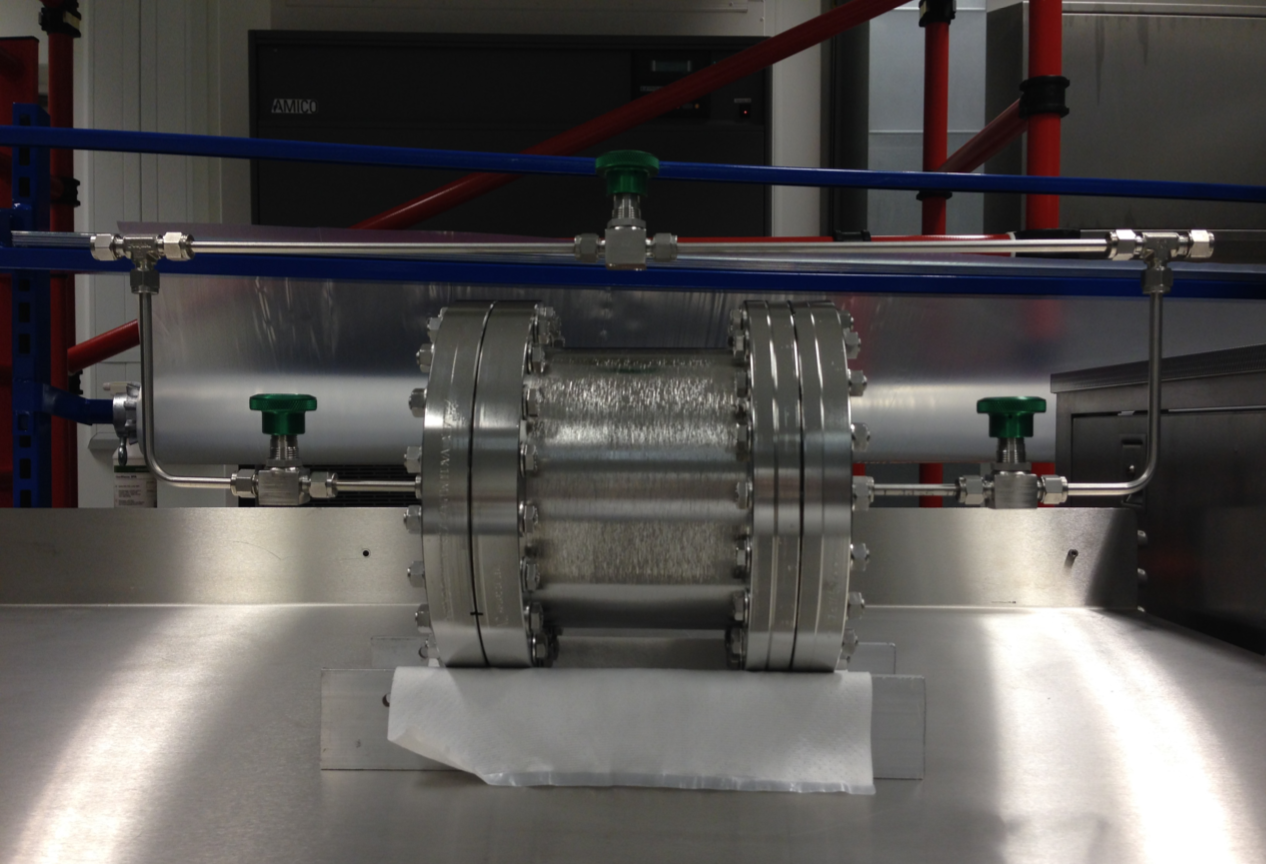
\includegraphics[scale=0.4]{Chapter_4/Figures/radon_system_chamber.png}
    \caption[A pictorial diagram of the 2.7 L stainless steel radon emanation chamber used to house samples for emanation.]
    {A pictorial diagram of the 2.7 L stainless steel radon emanation chamber used to house samples for emanation.}
    \label{fig:detector_chamber}
\end{figure}
%

A second mode of operation for the system uses 57\,g of activated carbon (a synthetic charcoal sourced from Carbo-Act International \cite{Pushkin:2018wdl}) as a radon collection trap. In larger emanation volumes, the radon is initially adsorbed into the cooled trap while the carrier gas passes through. The trap is then heated to release the radon and the carrier gas is then used to transfer the concentrated radon into the detector volume. The trapping efficiency for this setup has been measured to be $\approx 93$\% at 248\,K \cite{xin_2017}.


%%------------------------------$$
\section{LZ Radon Emanation Facilities}
\label{sec:otherradon}
%%------------------------------$$

The LZ radon emanation screening campaign utilises on four different facilities in measuring small and large scale samples: the UCL facility as detailed in section \ref{sec:ucl_radon_system}, South Dakota School of Mines and Technology (SDSM&T), University of Maryland and University of Alabama facilities. More in-depth discussion and details on these facilities and their operational methods are highlighted in \cite{lz_screening}.

The facilities operate under similar approaches in measuring emanation rates, where samples are initially enclosed in air-tight emanation chambers and the radon is harvested into their respective detectors after the equilibrium period. SDSM\&T and Maryland facilities make use of electrostatic PIN-diode detectors to measure the \alpha-particles from the \PoTOF{} and \PoTOE{} isotopes to reconstruct the radon emanation rate. The Alabama facility operates an organic liquid scintillator detector with a low-activity 3" Hamamatsu R-1307 PMT. Boil-off nitrogen with low intrinsic radon content is used to transfer the radon from an emanation chamber into 150 mL of scintillator. The emanation rate is reconstructed by detecting the scintillation light from the delayed \BiTOF-\PoTOF{} coincidences. 

LZ also makes use of two portable radon collection systems for equipment that is too large or are part of the construction in the SURF Surface Assembly Laboratory (SAL); i.e. radon emanation measurements from the ICV post skin region and TPC installation. Emanated radon is transferred to a cold trap consisting of copper beads or wool that is double-sealed and then transported by car or overnight shipping to the radon facility at SDSM\&T or University of Maryland. The collected radon is then transferred over into the respective radon detector with transfer efficiencies taken into account from portable-system specific calibrations. The activity is then reconstructed by correcting for the transportation time, transfer and detector efficiency. These portable systems were critical for measurements of radon emanation from the assembled LZ detector and from large instrumentation used in the circulation path. Harvesting of radon from the getter system at the SAL using one of the portable systems is displayed on figure \ref{fig:portable_radon_harvesting_system}.
%
\begin{figure}[b]
    \centering
    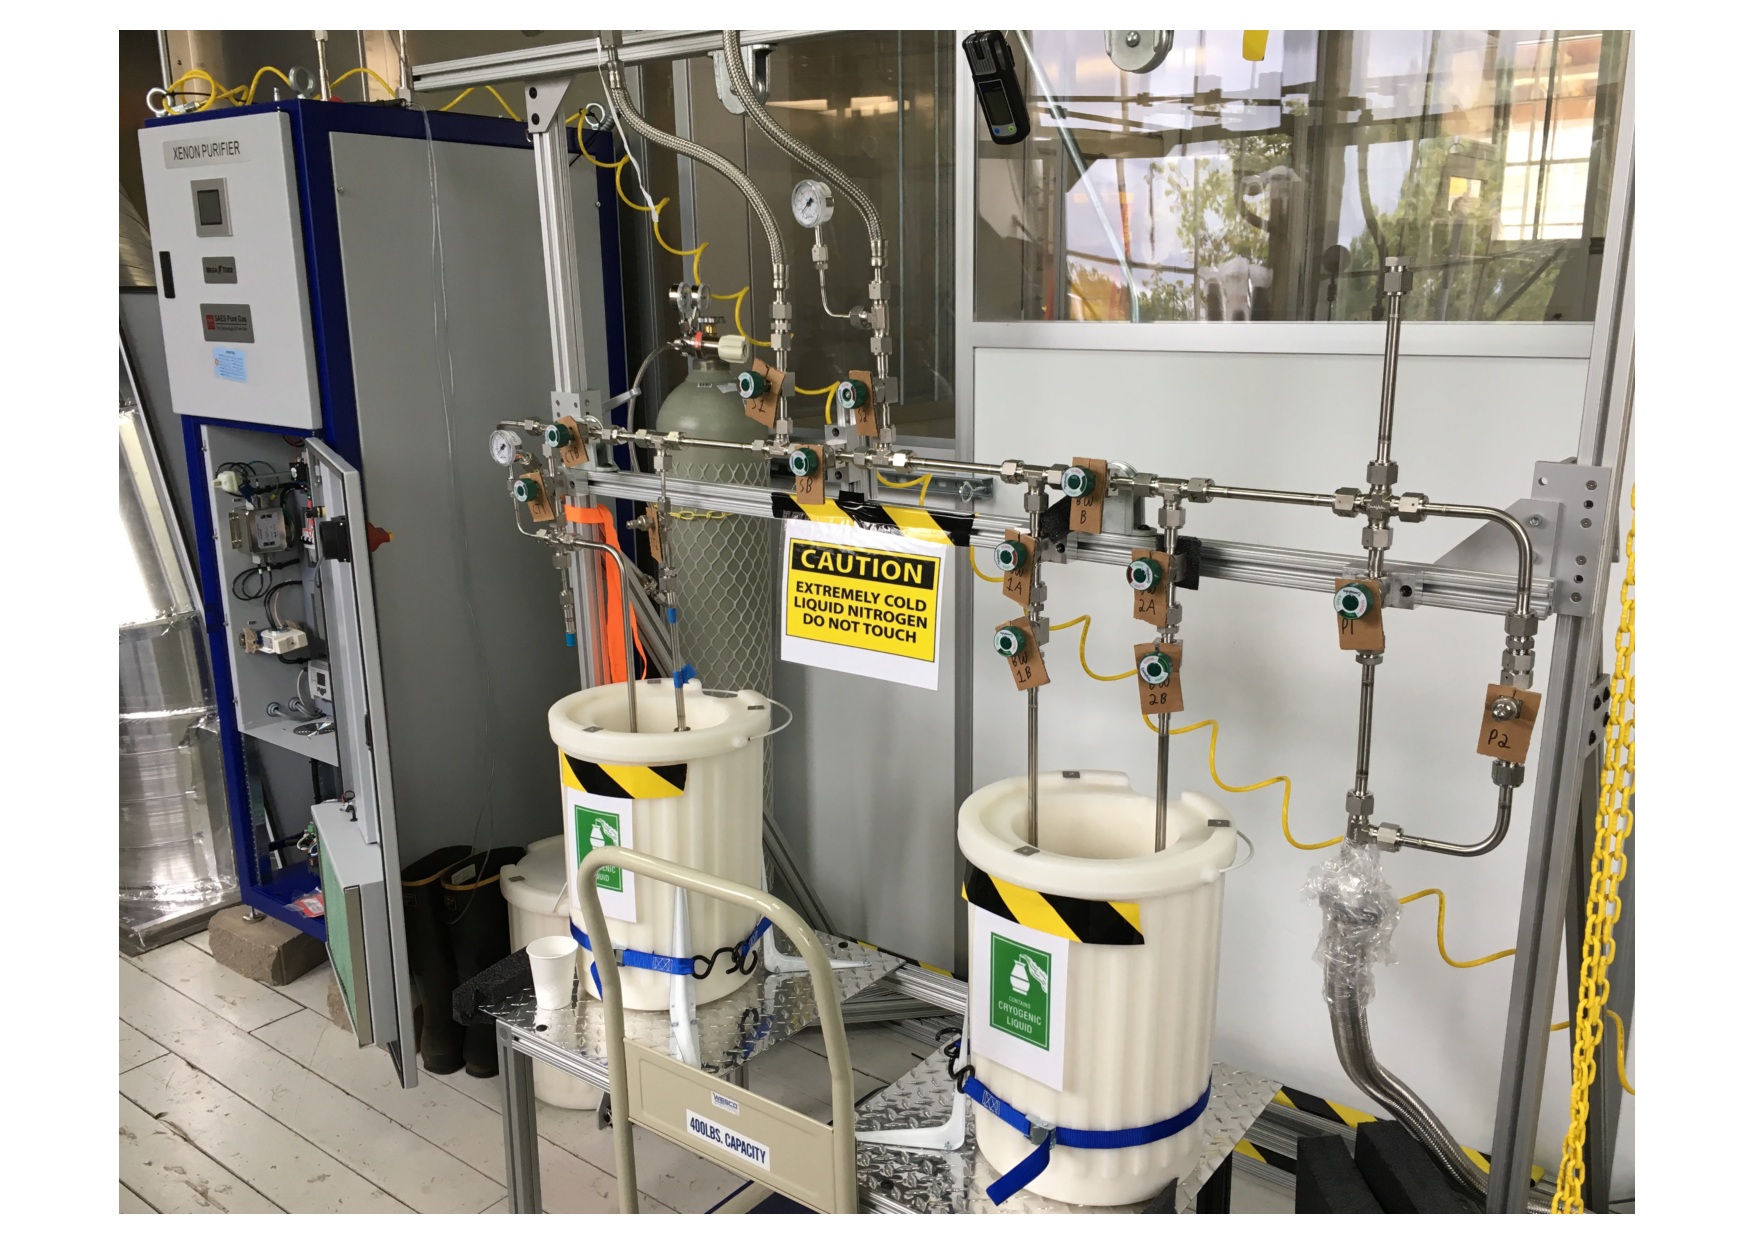
\includegraphics[scale=0.45]{Chapter_4/Figures/portable_system_operation.pdf}
    \caption[A pictorial diagram of the portable radon harvesting system used at the SAL for the getter radon emanation measurement.]
    {A pictorial diagram of the portable radon harvesting system used at the SAL for the getter radon emanation measurement. The emanated radon is collected by transferring through one of the traps held under LN$_{2}$ temperature. The trap is later transported to a radon emanation facility for counting.}
    \label{fig:portable_radon_harvesting_system}
\end{figure}
%


\subsection{Cross-Calibration Campaign}
\label{secsec:cross_cal}

%% NEEDS EDITING
The LZ collaboration performed cross-calibrations for the four radon facilities deployed as part of the assay program. A rubber sample previously screened by the EXO collaboration~\cite{Albert:2015nta, Miller:2017tpl} was assayed at each of the radon emanation facilities. Prior to the emanation period, the sample was prepared under the same conditions to reduce the chances of environmental contamination. The surface of the sample was scrubbed with isopropyl alcohol-soaked lint-free wipes and inspected with UV-light to ensure no presence of surface contamination. The emanation of the sample was \mathcal{O}(mBq) and was thus well above the minimal detectable activities of the radon systems. Table \ref{tab:ReDet} presents the results of the cross-calibration and a summary of key details of the LZ radon screening facilities. The EXO emanation results obtained through internal documentation indicated an activity of $4.94\pm0.07$ mBq. The cross-calibration results are provided as a ratio between the EXO activity and that measured with the various systems. All but the UCL emanation system agrees with the EXO results within error.
%
\begin{table}[hb!]
    \centering
    \caption{Comparison of the key highlights of the four radon emanation facilities used by LZ. The chambers detailed are those used in containing the sample material, where radon is collected. Some facilities operate two chambers as detailed below. Chamber blank rates detail the emanation rate from the chambers alone and are background subtracted for sample measurements. Detector efficiency represents the fraction of activity measured from the total radon inside the detecting volume; independent of chamber usage and transfer efficiency. The cross-calibration figures represent the reconstructed emanation rate of a standard rubber sample previously used by other collaborations. When not stated, overall uncertainties are estimated to be 10-20\%.}
    \label{tab:ReDet}
    \begin{adjustbox}{width=\textwidth,center}
    \tabcolsep=4pt
        \begin{tabular}{lcccccc}
        \toprule
        \multicolumn{1}{c}{\textbf{Detector}} & %0
        \textbf{Type} & %1
        \multirow{1}{*}{\textbf{Chamber Volumes}} &  %2
        \multirow{1}{*}{\textbf{Chamber Blank Rates}} &  %3
        \multirow{1}{*}{\textbf{Transfer Efficiency}} & %4
        \multirow{1}{*}{\textbf{Detector Efficiency}} & %5
        \multirow{1}{*}{\textbf{Cross-Calibration}}\\ %6
        & %0
        & %1
        \multirow{1}{*}{\textbf{[L]}} & %2
        \multirow{1}{*}{\textbf{[mBq]}} & %3
        \multirow{1}{*}{\textbf{[\%]}} & %4
        \multirow{1}{*}{\textbf{[\%]}} & %5
        \multirow{1}{*}{\textbf{[Measured/EXO--activity]}}\\ %6
        \hline
        \hline
        \vspace{-4mm}
        \\ 
        SDSM\&T & 
        PIN-diode & 
        \multicolumn{1}{c}{\begin{tabular}[c]{@{}c@{}}13\\ 300\end{tabular}} & \multicolumn{1}{c}{\begin{tabular}[c]{@{}c@{}}0.2\\ 0.2\end{tabular}} & 
        \multicolumn{1}{c}{\begin{tabular}[c]{@{}c@{}}94\\ 80\end{tabular}} & 
        25 & 
        \multicolumn{1}{c}{\begin{tabular}[c]{@{}c@{}}0.89$\pm$0.15\\ 1.11$\pm$0.28\end{tabular}}
        \vspace{2mm}
        \\ 
        Maryland & 
        PIN-diode & 
        4.7 & 
        0.2 & 
        96 & 
        24 & 
        1.13 $\pm$ 0.19
        \vspace{2mm} \\
        UCL & 
        PIN-diode & 
        \multicolumn{1}{c}{\begin{tabular}[c]{@{}c@{}}2.6\\ 2.6\end{tabular}} &
        \multicolumn{1}{c}{\begin{tabular}[c]{@{}c@{}}0.2\\ 0.4\end{tabular}} & 
        \multicolumn{1}{c}{\begin{tabular}[c]{@{}c@{}}97\\ 97\end{tabular}} & 
        30 & 
        1.53$\pm$0.15
        \vspace{2mm} \\ 
        Alabama & 
        Liquid Scint. & 
        \multicolumn{1}{c}{\begin{tabular}[c]{@{}c@{}}2.6\\ 2.6\end{tabular}} &
        \textless{}0.4 & 
        34 &
        36 & 
        0.83$\pm$0.17
        \\
        \bottomrule
        \end{tabular}
    \end{adjustbox}
\end{table}
%

An explanation for this systematic could be the exposure of the sample to radium rich air, hence increasing the radon activity of the sample. Furthermore, the UCL system was calibrated with a 2.5 Bq source in comparison to the very low activities measured from most of the samples. Another issue could be the assumption that this high activity calibration still holds at low activities. Further work on this will need to be conducted. In order to verify whether this discrepancy was due to a mishandling of the sample, or truly a systematic uncertainty of the ULC system, a second cross-calibration is currently underway. Instead of using a rubber sample, 20 titanium rods were emanated in all of the radon emanation facilities. The preliminary results indicate that the activity observed by the UCL system is still relatively higher than the rest of the facilities. The analysis of this sample needs further work, hence the results are not yet published. Due to the uncertainties in understanding why the UCL system is behaving in such a way, it is difficult to conclusively explain this behavior and with the preliminary results from the titanium rods, this discrepancy is taken as a systematic and applied to all LZ results that were measured using the UCL system, applying a corrective factor of $0.65\pm0.06$ to these measurements.


%%------------------------------$$
\section{Radon Emanation Measurements for LZ}
\label{sec:uclradon}
%%------------------------------$$

Screening key components of the LZ detector that are in direct contact with the xenon circulation system for radon emanation has been one of the primary focal points in the LZ screening campaign. The UCL radon emanation system has been used extensively for several of these key measurements; including various PMT bases that are located inside the ICV and the TPC, the raw titanium and titanium welding used for the cryostats and several other structural segments with the ICV, and various other items. This section will highlight some of these results in detail.


\subsection{PMT Bases}
\label{secsec:pmt_base_emanation}

The LZ detector will use a total of 500 3", 39 2" and 94 1" PMT bases, all of which reside in the xenon volume of the detector. The components used in these bases are mostly (both in mass and area) made up of Cirlex (Kapton) printed circuit boards (PCBs), solder, capacitors, resistors and receptacles; together adding up to a considerable surface area within the xenon. Assays of these individual components have previously been conducted with \gamma{}-screening and radon emanation to build a \textit{bottom-up} model of the expected radon from the fully assembled bases. The solder and the receptacles were excluded as they yielded low \UTTEe{} activities with \gamma-screening; and emanation results from the other components yielded a \textit{bottom-up} approximation of 1.01 mBq for all bases used in LZ. This corresponds to 1.65 \micro{}Bq and 1.25 \micro{}Bq per a 3" and 1" base respectively. The pictorial diagram of the 1" and 3" bases used in this study are shown in figure \ref{fig:1_and_3_inch_bases}.
%
\begin{figure}[b]
    \centering
    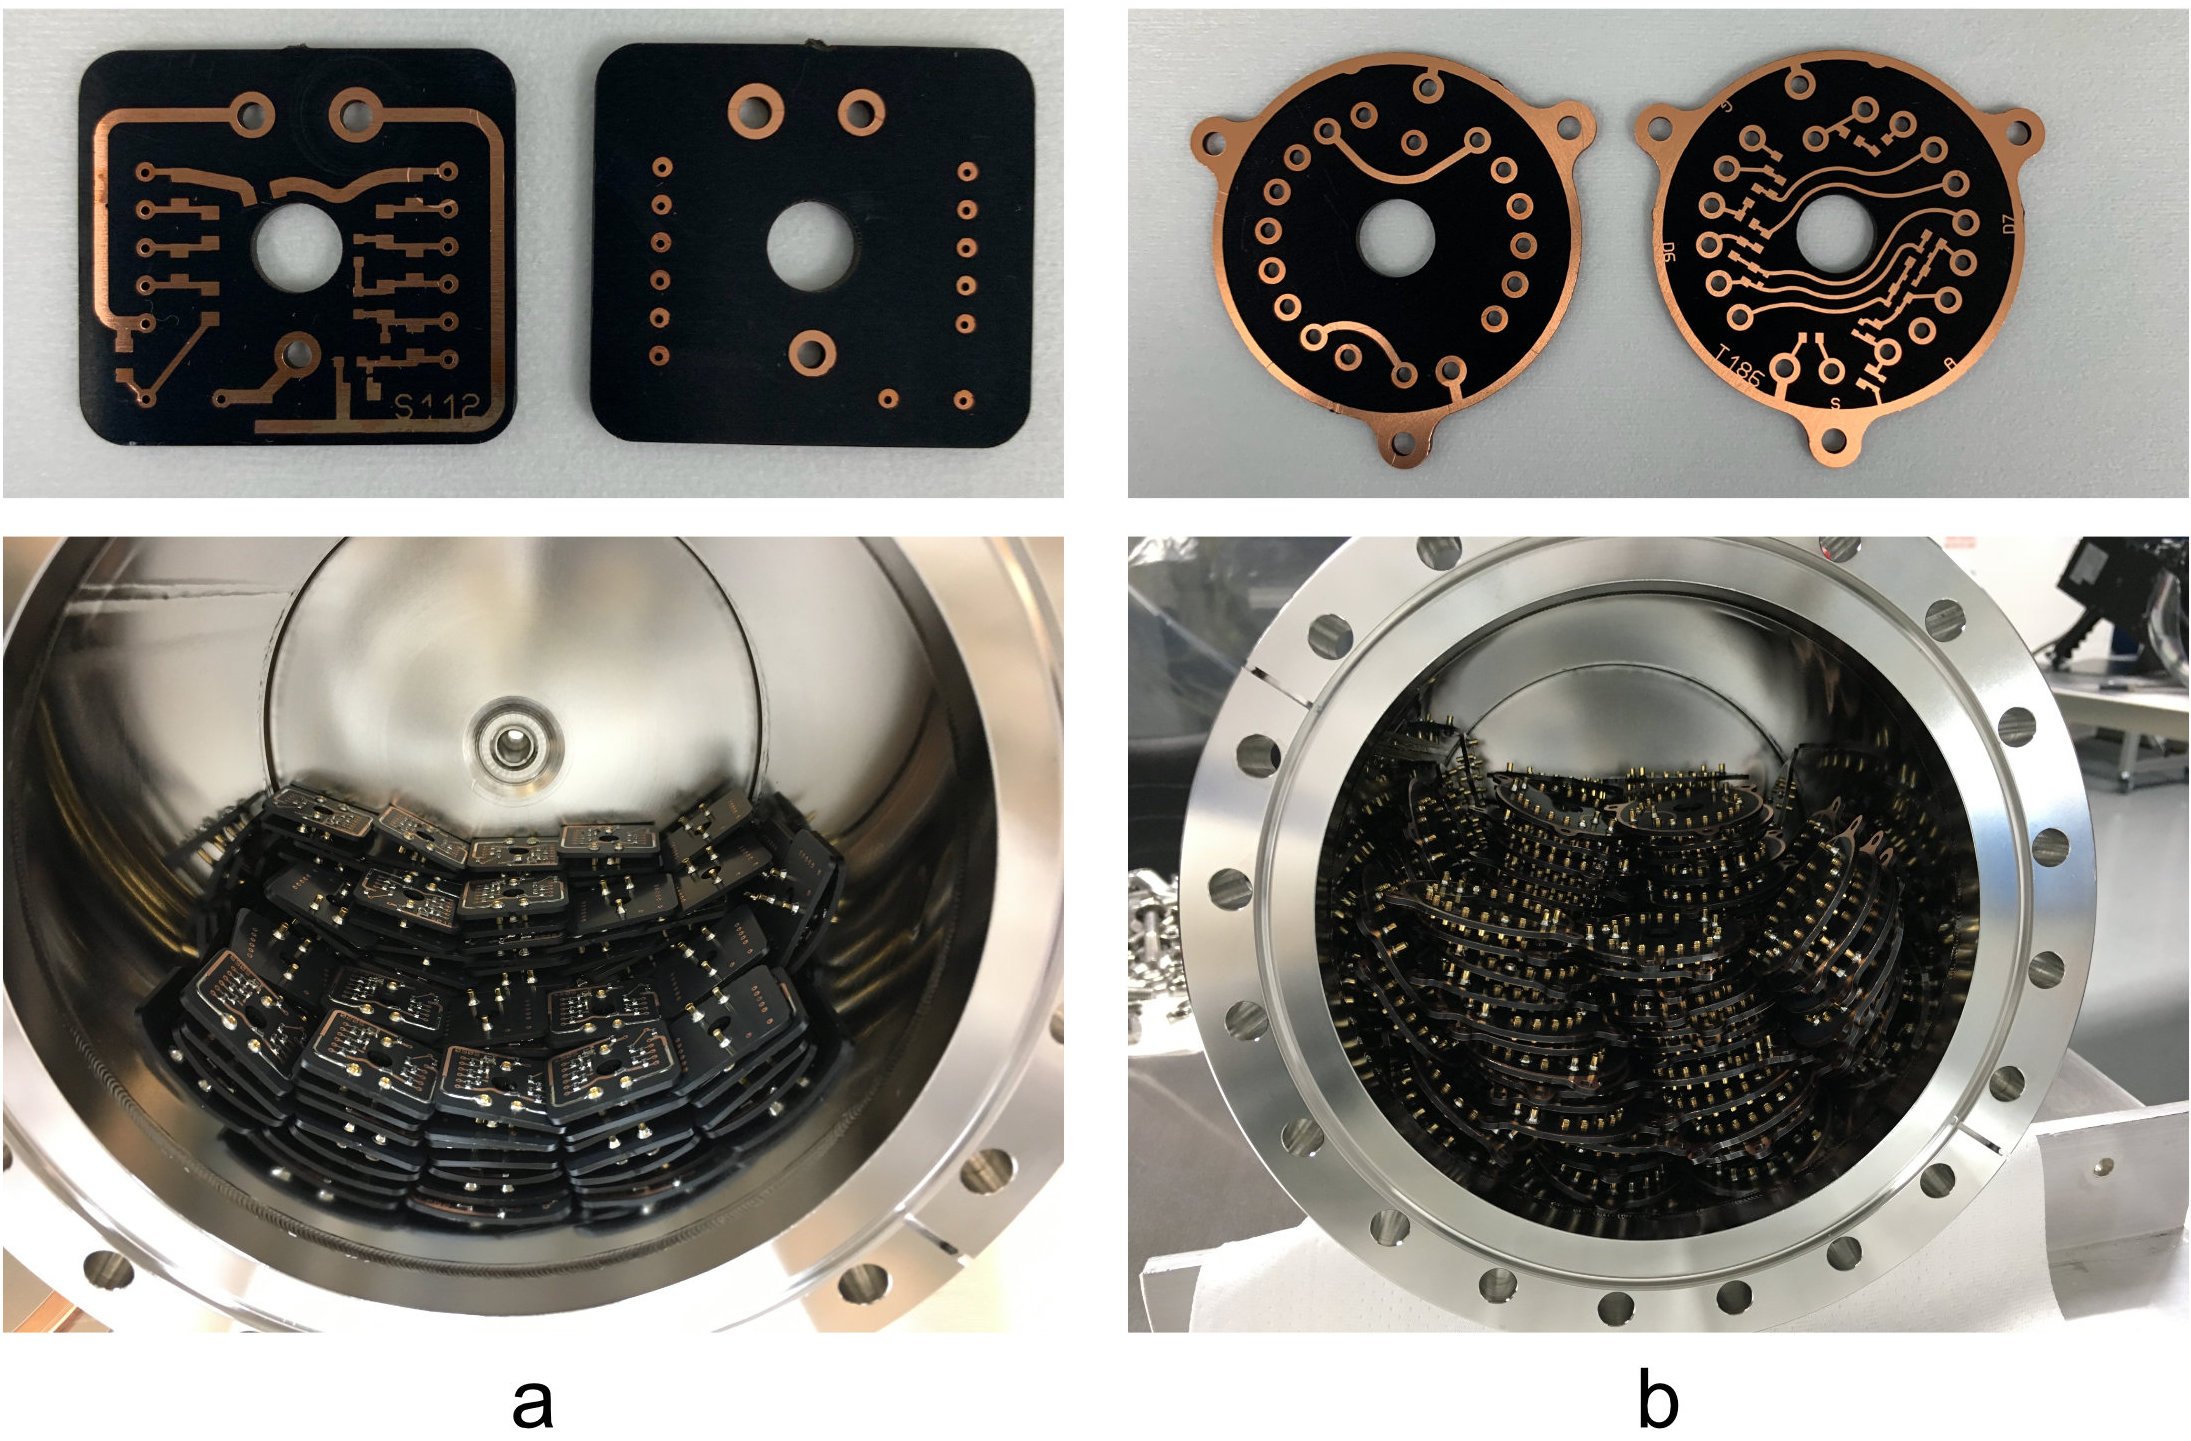
\includegraphics[scale=0.2]{Chapter_4/Figures/ucl_measurements/pmt_bases.jpg}
    \caption[A pictorial diagram of the 1" (a) and 3" (b) PMT base boards and their positioning within the UCL emsanation chamber.]
    {A pictorial diagram of the 1" (a) and 3" (b) PMT base boards and their positioning within the UCL emsanation chamber.}
    \label{fig:1_and_3_inch_bases}
\end{figure}
%
%
\begin{table}[h]
\centering
\caption{Relation of components in the different kind of LZ bases. The Cirlex mass is proportional to the Cirlex surface since all the bases are made of a 1.5 mm thick Cirlex PCB. All resistors and capacitors have the same dimensions. Regarding the solder, please refer to the text.}
\label{tab:pmt_base_components}
\vspace{1mm}
\renewcommand{\arraystretch}{1.2}
    \begin{tabularx}{.9\linewidth}{@{\extracolsep{\fill}}llll}
    \toprule
    
    \textbf{Components} & %1
    \textbf{3" PMT Bases} & %2
    \textbf{2" PMT Bases} & %3
    \textbf{1" PMT Bases} & %4
    
    \hline
    \hline
    
    Cirlex PCB	    & 3300 mg       & 3300 mg       & 1680 mg   \\
    Resistors       & 15 units      & 15 units      & 13 units  \\       
    Capacitors	    & 5 units       & 5 units       & 3 units   \\        
    Receptacles	    & 19 units      & 20 units      & 3 units   \\       
    Solder  	    & 180 mg        & 180 mg        & 300 mg    \\       
    
    \bottomrule
    \end{tabularx}
\end{table}


%

Although the bases are all constructed from the same material, they do differ in the quantity of components use. These differences are highlighted in table \ref{tab:pmt_base_components}. The 3" and 2" PMT bases are essentially identical in size and component use, with the only minor difference being the additional receptacle used on the 2" PMT base. Hence, the results obtained for 3" bases are also assumed for 2" bases. The 1" bases are substantially different and hence were separately screened. The 180 mg value quoted for the total mass of solder used per 3" base was measured by weighing the bases before and after solder was applied. However, the same approach was not conducted for the 1" bases. The difficulty in doing a similar measurement was due to the variation in the amount of solder used for an individual 1" base. The 1" bases use similar number of components and in addition to this, they contain two reinforced solder tracks, hence a 300 mg was adopted as a best estimate. 


\subsubsection{Emanation of 3" Bases}

A total of 124 3" bases were packaged inside radon tight bags at the Imperial College cleanroom and transported to the radon facility cleanroom at UCL. Each base was then carefully taken out of the radon tight packaging and placed inside the emanation chamber with caution to avoid scratching or damaging base components. After the emanation period of 15 days, the radon was transferred into the electrostatic detector and measurements on the decay rates of \PoTOF{} and \PoTOE{} were made. A second measurement was followed before the bases were transported back to Imperial College. The pre-corrected \PoTOF{} rates from these two measurements are shown in figure \ref{fig:3_inch_pmt_base_results}. Although not provided, the \PoTOE{} rates were checked for completeness and was found to agree within error with those obtained from \PoTOF{}. The output from the \PoTOF{} result was then corrected by applying the detector efficiency corrections detailed in section \ref{sec:detector_efficiency} to give a total radon emanation rate of $0.62\pm0.11$ mBq and $0.70\pm0.11$ mBq for 124 3" bases for the first and the second measurement respectively. 
%
\begin{figure}[h!]
    \centering
    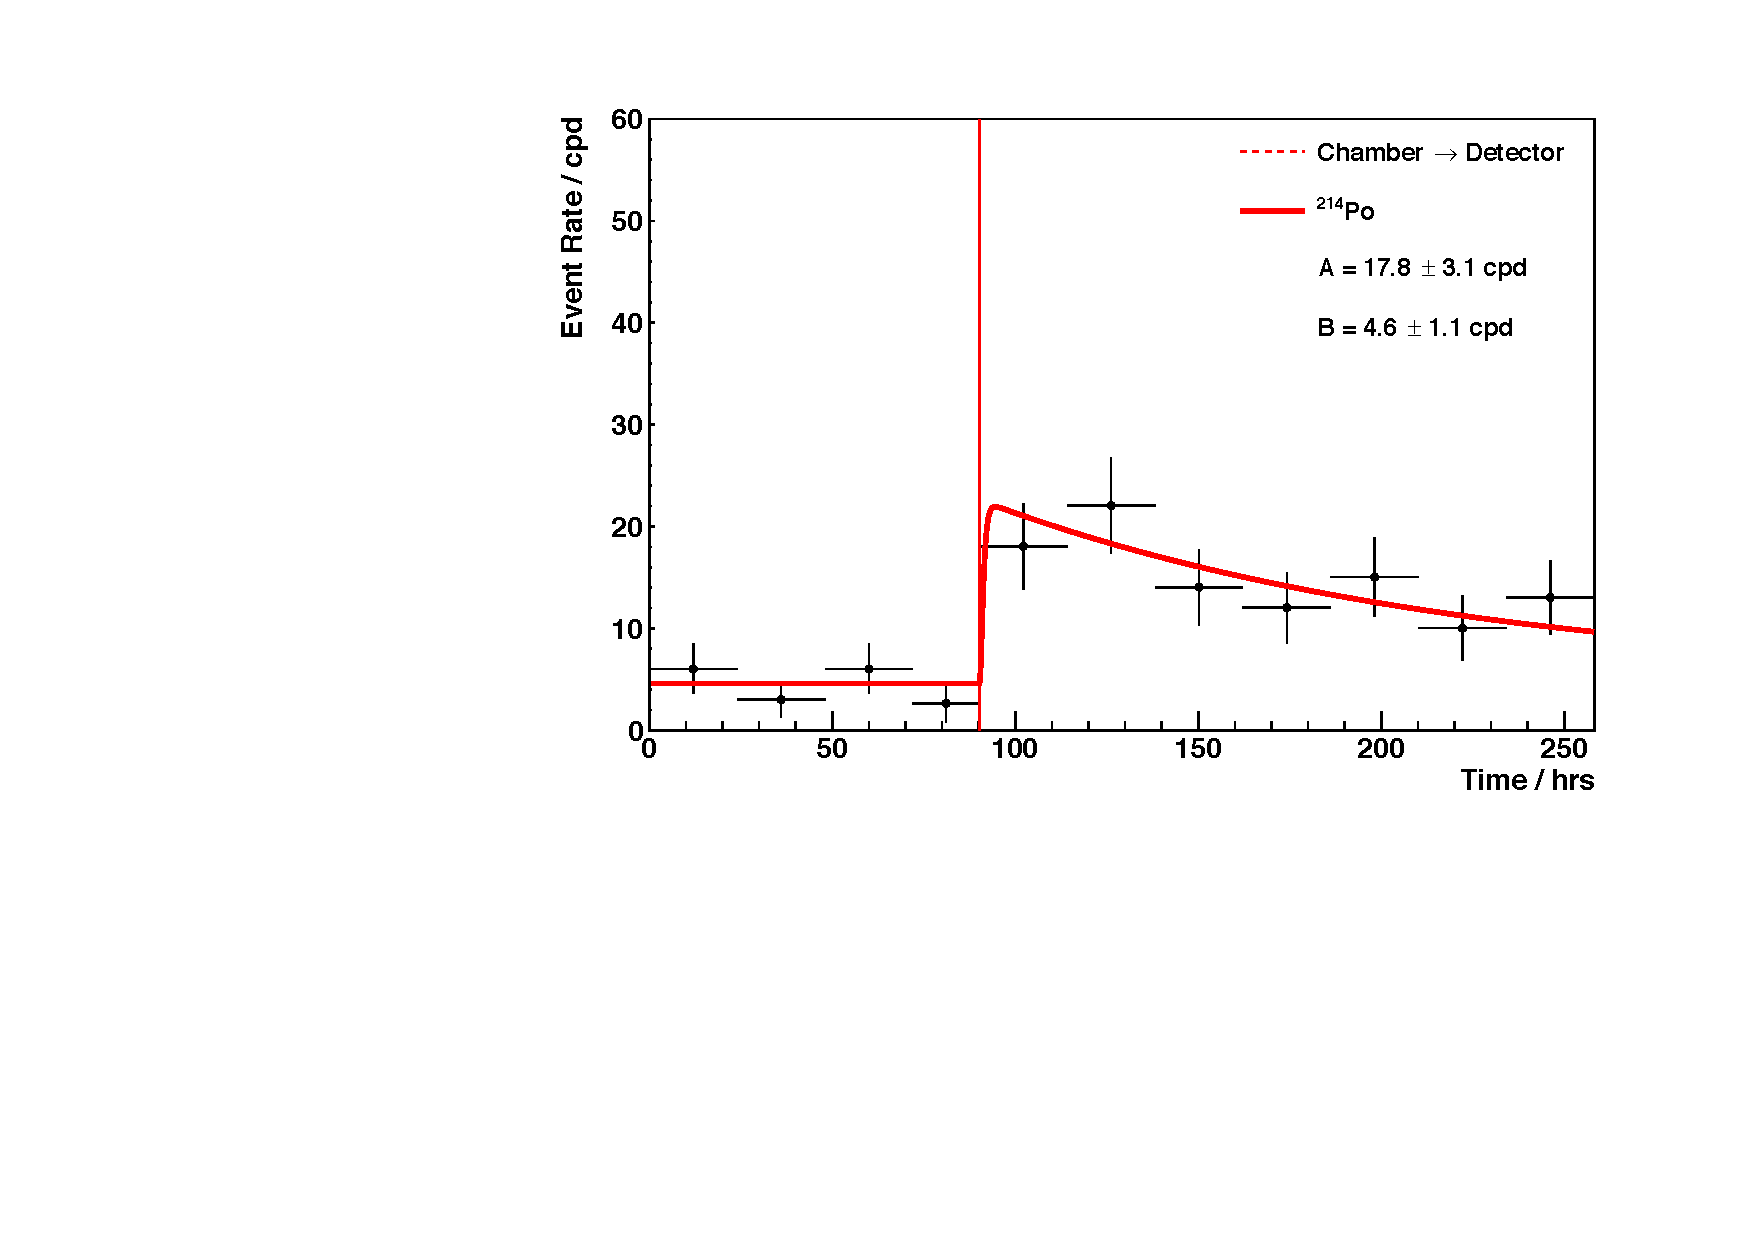
\includegraphics[scale=0.42]{Chapter_4/Figures/ucl_measurements/3_inch_bases_first_Po214.pdf}
    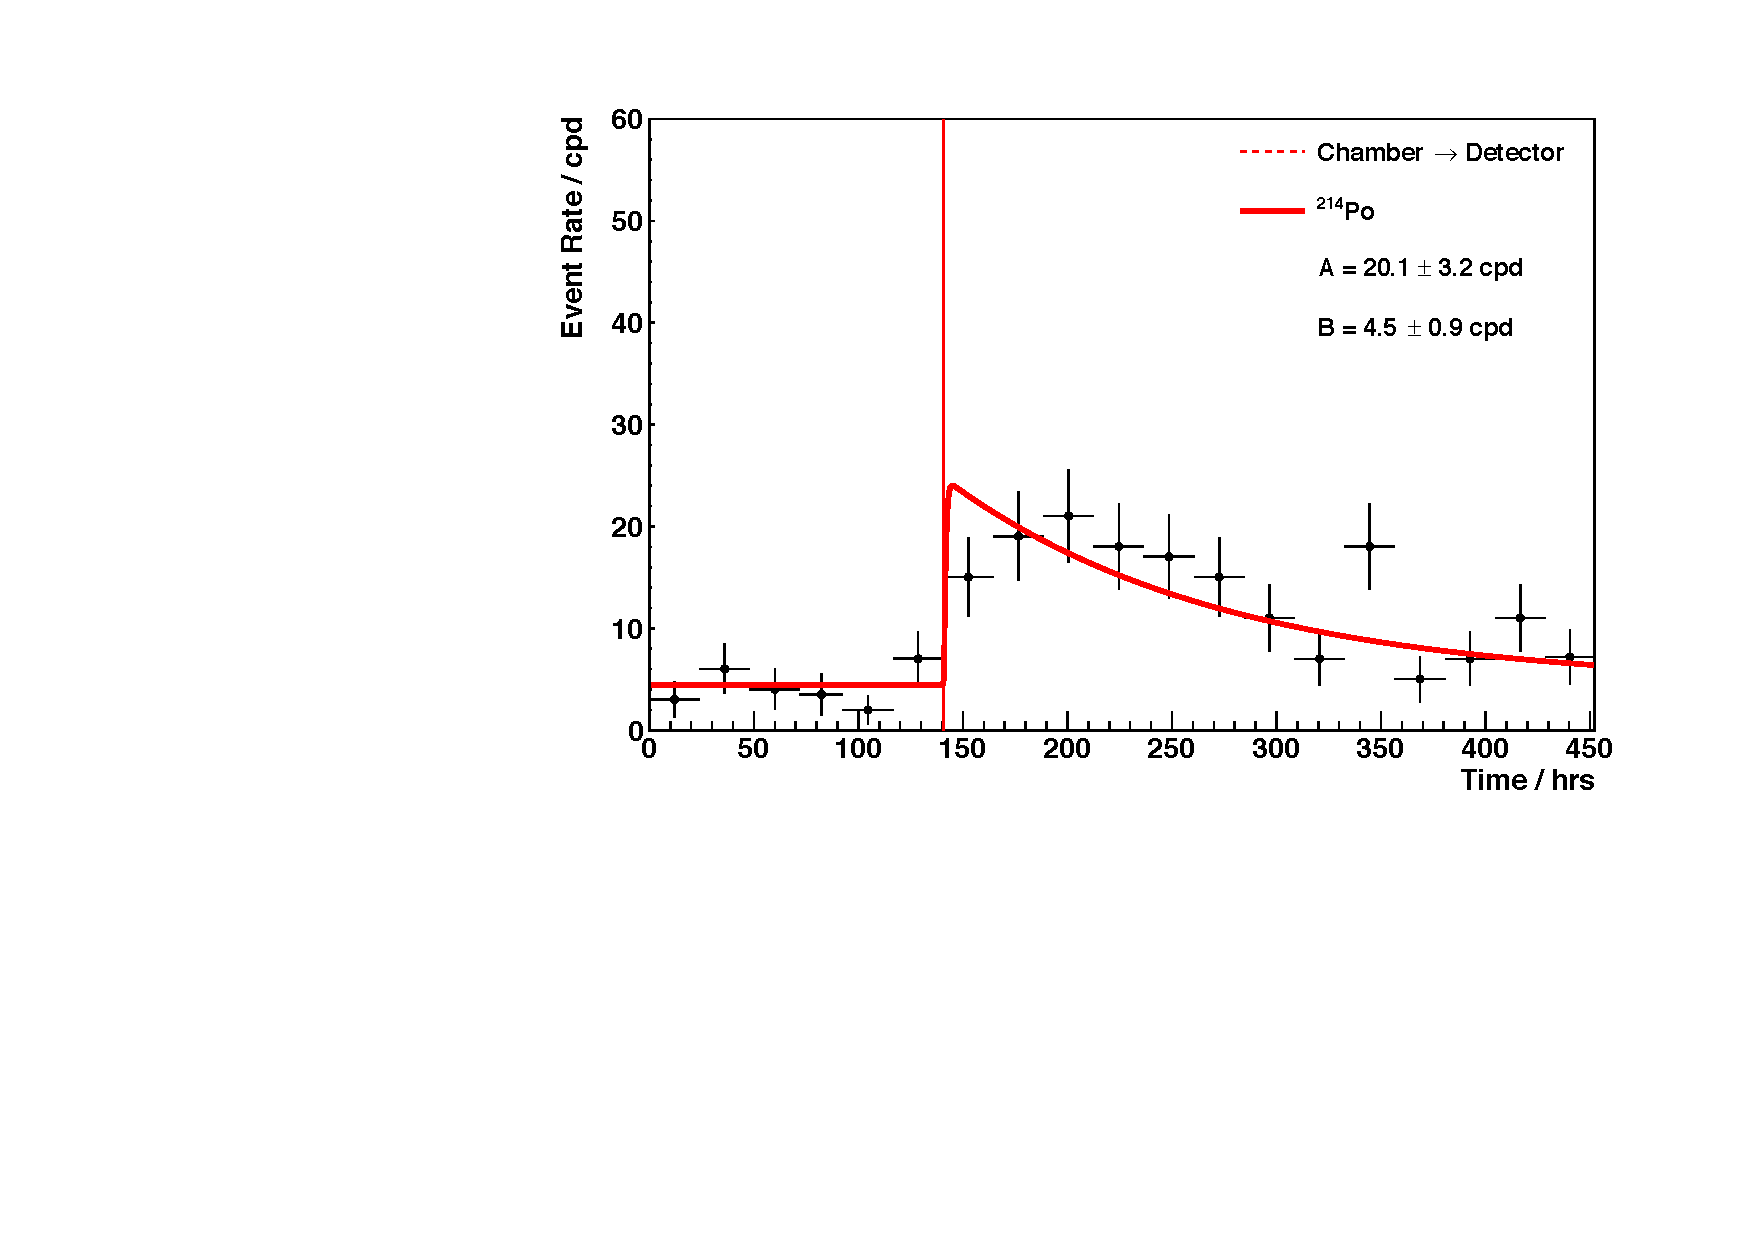
\includegraphics[scale=0.42]{Chapter_4/Figures/ucl_measurements/3_inch_bases_second_Po214.pdf}
    \caption[Pre-corrected \PoTOF{} event rate results obtained from the two measurements made on the 124 3" PMT bases screened using the UCL radon emanation system.]
    {Pre-corrected \PoTOF{} event rates of 124 3" PMT bases screened using the UCL radon emanation system. The bases were prepared and cleaned with a procedure identical to those used in the LZ detector.}
    \label{fig:3_inch_pmt_base_results}
\end{figure}
%


\subsubsection{Emanation of 1" Bases}

The emanation results from the 3" bases yielded a large discrepancy between the bottom-up estimations, hence 120 1" bases were emanated at the UCL facility to determine the radon background from these bases, as the bottom-up estimations were no longer reliable for the LZ background projections. Furthermore, the instrumental differences between the 3" and 1" could help understand why such a large discrepancy was observed; whether some of the components making up the bases were more radioactive than expected. These bases were treated identically to the 3" bases; initially cleaned at the Imperial College cleanroom to remove any surface contamination, and later transported to the UCL facility in radon tight packaging to minimise radon plate-out. After an emanation period of two weeks, en emanation measurement was conducted. The pre-corrected results obtained for \PoTOF{} and \PoTOE{} rates are in agreement within error and their rates within the detector are shown in figure \ref{fig:1_inch_pmt_base_result}. The output from the \PoTOF{} decay rate is then corrected by applying the detector efficiency corrections and the radon emanation rate of 120 1" bases are calculated to be $0.53\pm0.11$ mBq.
%
\begin{figure}[h!]
    \centering
    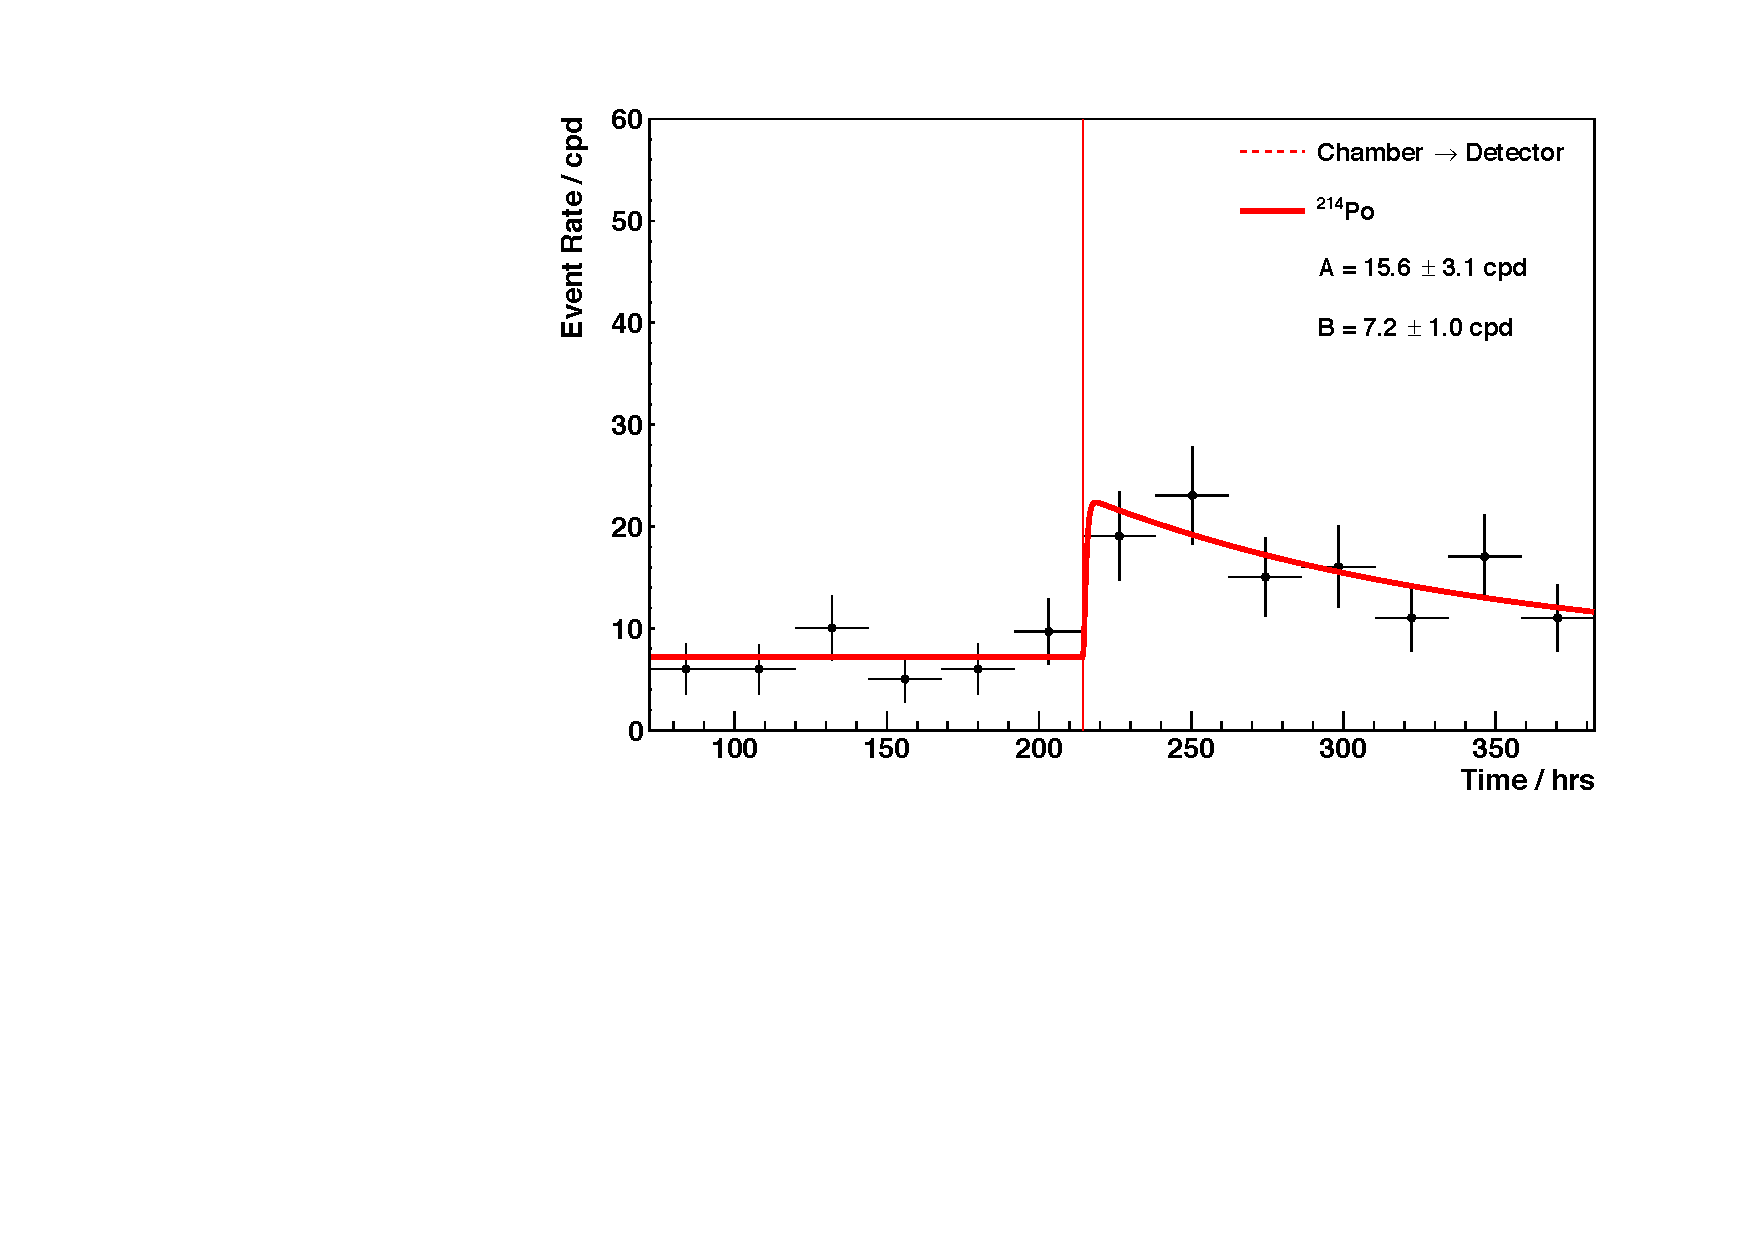
\includegraphics[scale=0.42]{Chapter_4/Figures/ucl_measurements/1_inch_base_Po214.pdf}
    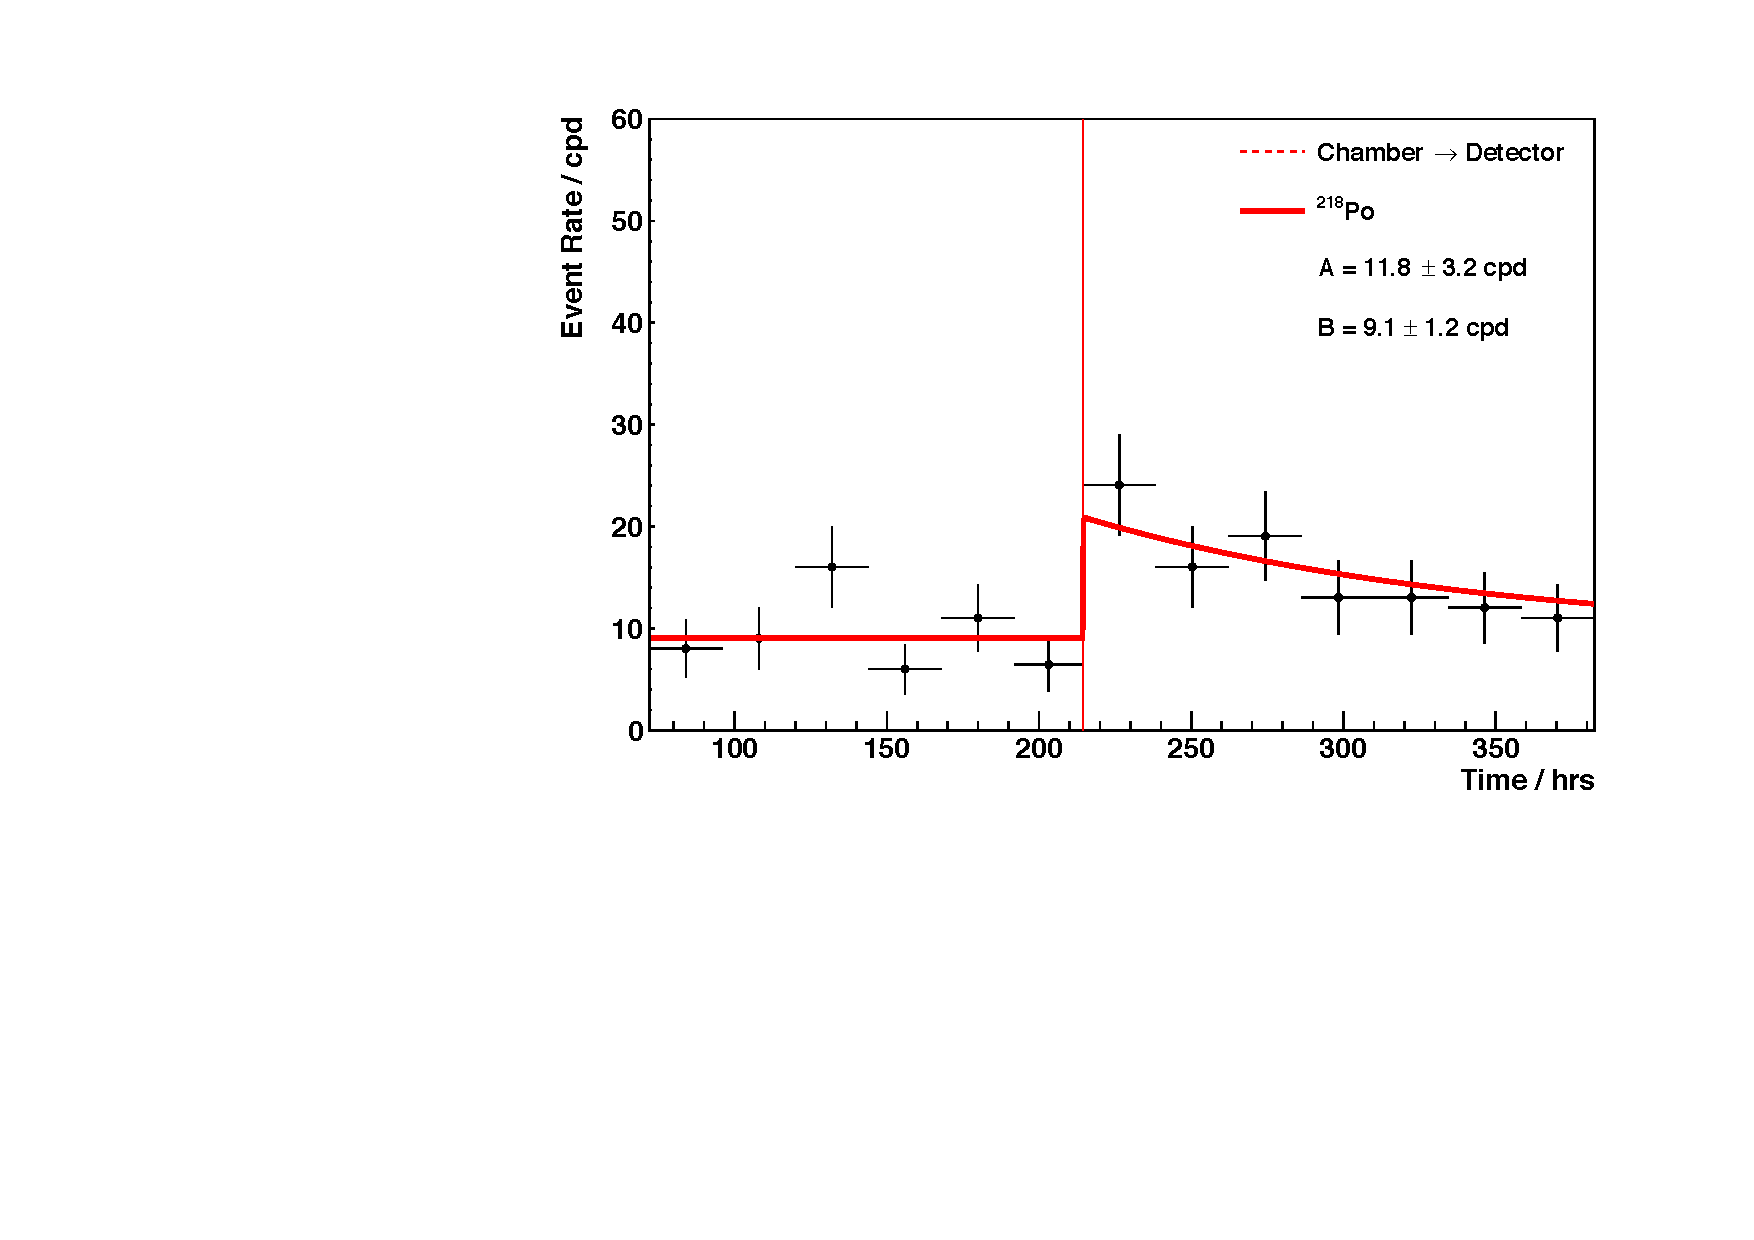
\includegraphics[scale=0.42]{Chapter_4/Figures/ucl_measurements/1_inch_bases_Po218.pdf}
    \caption[Pre-corrected \PoTOF{} (left) and \PoTOE{} (right) event rates of 120 1" PMT bases screening, representative of those that are used in LZ.]
    {Pre-corrected \PoTOF{} (left) and \PoTOE{} (right) event rates of 120 1" PMT bases screened using the UCL radon emanation system. The bases were prepared and cleaned with a procedure identical to those used in the LZ detector.}
    \label{fig:1_inch_pmt_base_result}
\end{figure}
%


\subsubsection{Discussion \& Conclusion}

%
\begin{table}[b]
\centering
\caption
[HPGe screening of rock, shotcrete and gravel samples from the Davis cavern laboratory.]
{Radon emanation results as obtained from the UCL system for the 3" and the 1" bases with bottom-up comparisons. All the results are given per respective base. A measurement from the XENON1T collaboration for 3" bases with almost identical design and component usage is provided for comparison \cite{Natascha}.}
\label{tab:pmt_base_results}
\vspace{1mm}
\renewcommand{\arraystretch}{1.2}
    \begin{tabularx}{.9\linewidth}{@{\extracolsep{\fill}}lll}
    \toprule
    
    \textbf{Measurement} & %1
    \textbf{3" Bases [\micro{}Bq/base]} & %2
    \textbf{1" Bases [\micro{}Bq/base]} & %3
    
    \hline
    \hline
    
    Bottom-up 	            & 1.65\pm0.56$      & 1.25\pm0.47       \\
    1$^{st}$ Measurement    & $5.00\pm0.86$     & $4.42\pm0.90$     \\       
    2$^{nd}$ Measurement	& $5.65\pm0.90$     & -                 \\        
    \hline
    Averaged	            & $5.33\pm0.63$     & $4.42\pm0.90$     \\       
    XENON1T Bases           & $3.0\pm0.6$       & - \\
    
    \bottomrule
    \end{tabularx}
\end{table}


%
The radon emanation results from the 3" and the 1" bases, along with their bottom-up estimates are highlighted in table \ref{tab:pmt_base_results} for comparison. The results indicate a radon emanation activity of 5.33 \micro{}Bq and 4.42 \micro{}Bq per 3" and 1" base; which is 3.68 \micro{}Bq and 3.17 \micro{}Bq above the bottom-up estimation respectively. Although the 1" bases have less Cirlex and electronic components, the activity in comparison to the 3" bases are relatively high, suggesting the solder to have a non-zero activity comparable to some of the components taken into account. In assuming the 3" bases emanation rate also applied to the 2" bases, the contributions from all LZ bases together returns a total contribution of $3.21 \pm 0.35$ mBq.  Furthermore, a cross-calibration campaign between all of the radon facilities used by LZ, as highlighted in section \ref{sec:otherradon}, indicated an upwards systematic for the UCL radon emanation system of 1.53 when compared to the base rate of the sample. In considering this systematic, the total radon emanation rate of the bases go down to $2.10\pm0.23$ mBq. This equates to an activity of $3.38\pm0.41$ \micro{}Bq/[3” base]---in good agreement with the result obtained by XENON1T \cite{Natascha}. It is important to note that these values do not assume any reduction in rate due to temperature and the actual rate in LZ may be lower due a temperature suppression.


\subsection{Cryostat Titanium \& Titanium Welding}
\label{secsec:titanium_emanation}

In the early stages of the LZ experiment, an extensive R\&D campaign was conducted to source and produce enough titanium for the cryostat vessels of the detector. The ICV and the OCV, which contain the TPC and the 10 tonnes of LXe, make up a significant bulk of the LZ detector. Due to their scale and proximity to the TPC, it was necessary to ensure ultra-low levels of radiopurity for \UTTE{} and \ThTTT{} isotopes as well as \KFZ{} and \CoSZ{}. A detailed analysis using ICP-MS and gamma-ray spectroscopy of 22 different titanium samples was conducted, and the sample of the HN3469 product manufactured by TIMET was found to have the lowest background. The measured activities for \UTTEe{}, \ThTTTe{}, \CoSZ{} and \KFZ{} from the sample are significantly lower than requirements and were the lowest reported to date \cite{LZ_titanium_selection}. 

Assuming chemical equilibrium within the titanium for both the uranium and thorium series, the ultra-low activities measured by the ICP-MS facility for \UTTEe{} (<0.13 ppb) and \ThTTTe{} (0.069(7) ppb) lead to a negligible amount of radon emanation, with the assumption that diffusion would be heavily suppressed due to the dense metallic nature of titanium. To this day, there are no known measurement of radon emanation from titanium, however, results from steel sheets and welding have previous been reported by the GERDA collaboration with activities in $\mathcal{O}(10)$ \uBqms \cite{osti_20719228, ZUZEL2009889}. 

Although the OCV is relevant for \grays, backgrounds for radon emanation is only expected from the ICV and its inner content. The ICV uses a total of 950 kg of titanium with several other titanium pieces used for structural support of PMTs, both in the skin region and within the TPC. Furthermore, the ICV is made up of several smaller segments welded together using $\sim$6 kg of titanium welding rods. After the installation of the skin region at SURF, the ICV was sealed and left to emanate. The results obtained from the harvested radon from the ICV indicated an emanation rate of $28.3\pm2.0$ mBq; in comparison to this, the expected bottom-up emanation from individual measurements of components within the ICV was only $2.3^{+3.7}_{-0.9}$ mBq. This large discrepancy was unexpected and prompted a radon screening campaign to examine some of the potential sources; emanation from dust accumulation and from unaccounted components (i.e. titanium cryostat and welding). 

To examine radon emanation from the welded surface and the raw titanium surface, a 7 mm titanium plate welded with titanium and several titanium cutouts from the OCV were shipped to the UCL radon facility. A pictorial diagram of these two samples can be seen in figure \ref{fig:titanium_welding_sheets} just before their respective emanation periods. The welded block was originally constructed from the LZ stock to study abnormally high ICP-MS measurements, detailed in \cite{lz_screening}.
%
\begin{figure}[t]
    \centering
    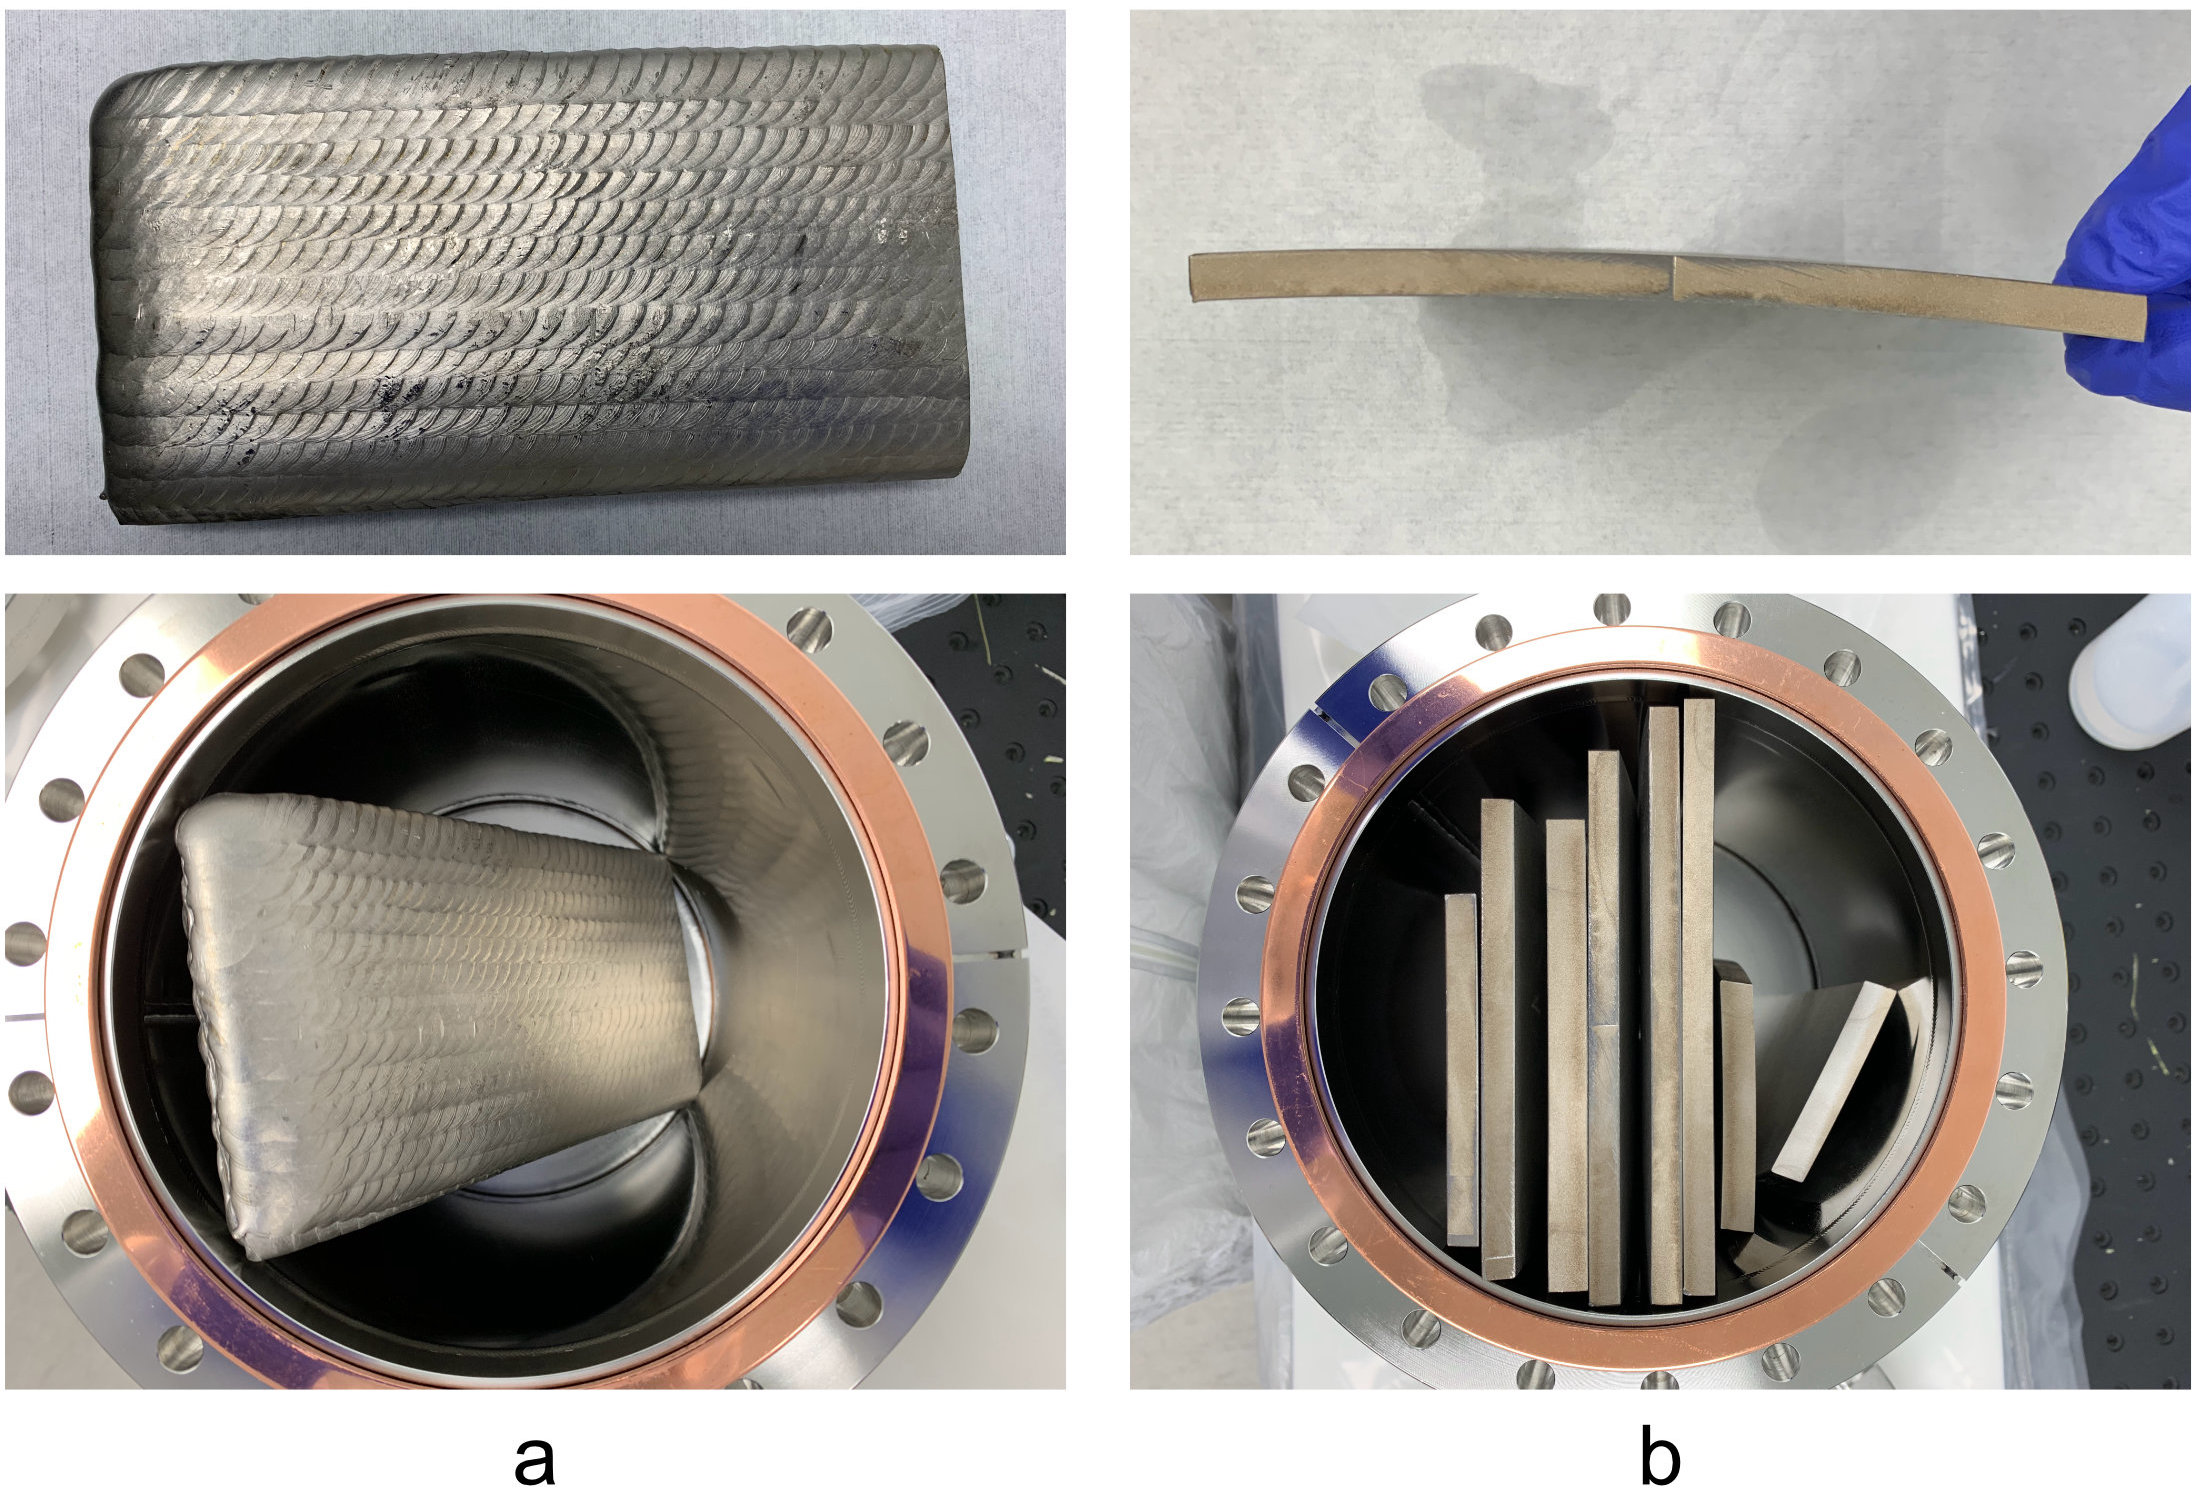
\includegraphics[scale=0.2]{Chapter_4/Figures/ucl_measurements/titanium_and_welding.jpg}
    \caption[A pictorial diagram of welded titanium block and the titanium sheets cut-off from the LZ OCV.]
    {A pictorial diagram of welded titanium block (a) and the titanium sheets (b) cut-off from the LZ OCV.}
    \label{fig:titanium_welding_sheets}
\end{figure}
%


\subsubsection{Titanium Welding}

To examine radon emanation from a titanium welded surface, a sample of 7 mm Ti plate with a large TIG weld on both sides with a total welding surface area of 325 cm\squared{} was assayed at the UCL facility. The sample is one of four blocks originally prepared for quality control during the ICV and OCV manufacturing. Studies on this sample using ICP-MS yielded concentration of $0.16\pm0.04$ ppb \UTTEe{} and $3.20\pm0.16$ ppb \ThTTTe{}. The higher levels of \ThTTTe{} were attributed to the inadvertent use of thoriated electrodes, which was later corrected as a result of this study with no impact on background. The final welding used inside the ICV was from the same titanium stock but used lanthanated elecrodes. \RnTTT{} is strictly coming from the \UTTE{} decay chain and hence the results highlighted here are assumed to apply to lanthanated welding. Two sets of measurements were performed on the welded block: emanation prior to etching and post etching by AstroPak---a certified professional precision cleaning company. Results obtained for the pre-etched and post-etched block are shown in figure \ref{fig:ti_pre_etched_welded_block_results} and \ref{fig:ti_post_etched_welded_block_results}, respectively. Pre-etched block was measured once, whereas the post-etched block was measured twice.
%
\begin{figure}[h!]
    \centering
    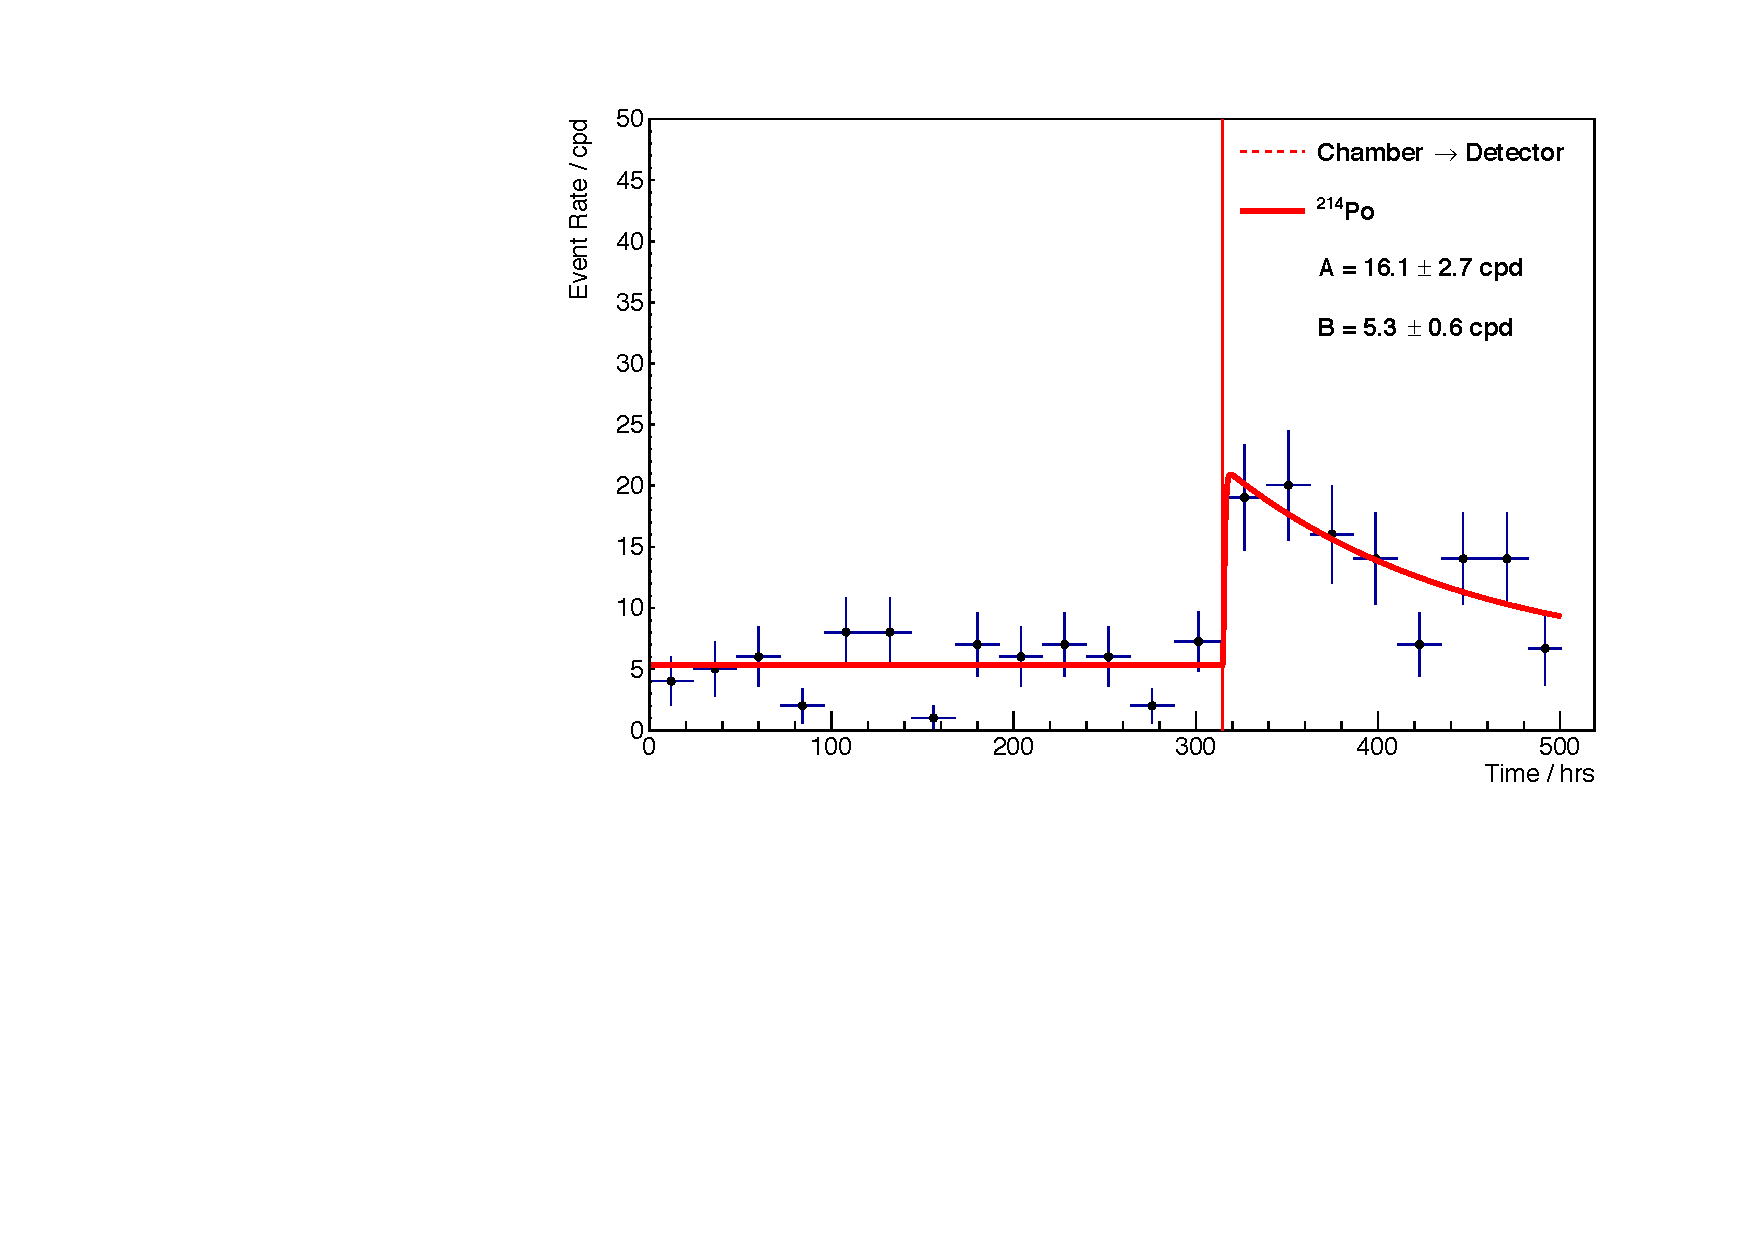
\includegraphics[scale=0.42]{Chapter_4/Figures/ucl_measurements/titanium_welding_block_pre_etching_1_Po214.pdf}
    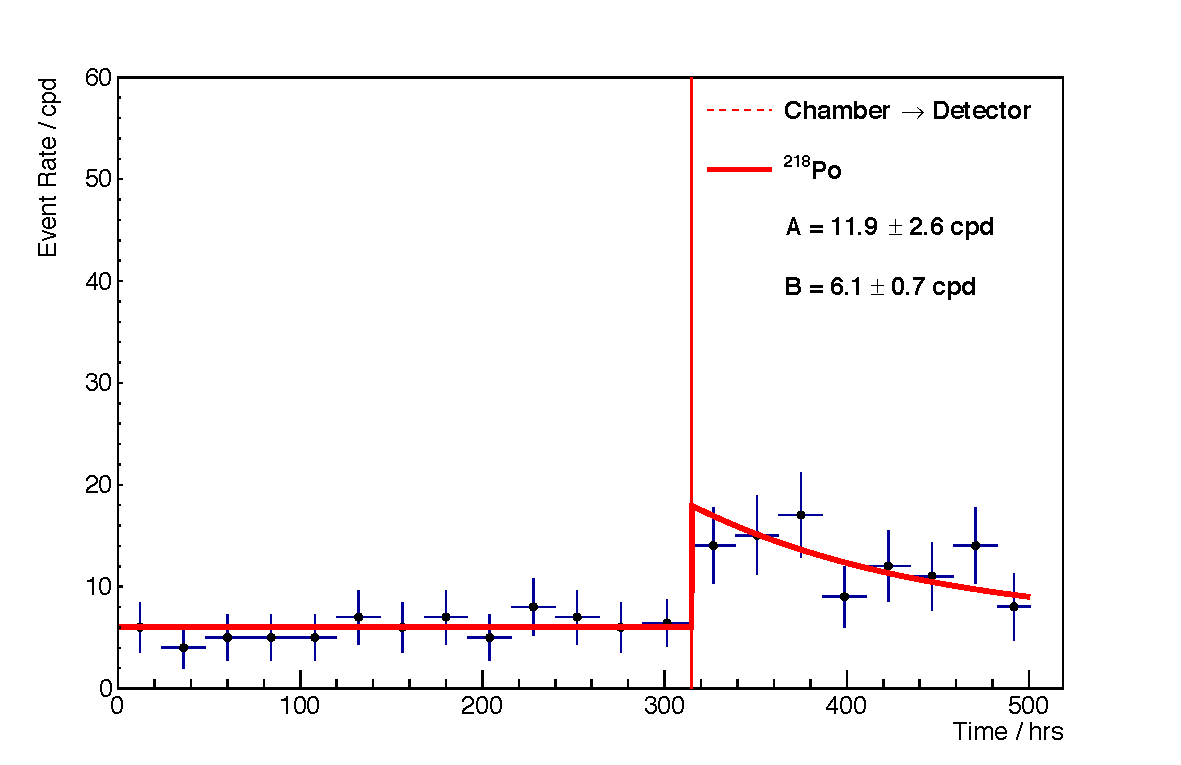
\includegraphics[scale=0.42]{Chapter_4/Figures/ucl_measurements/titanium_welding_block_pre_etching_1_Po218.pdf}
    \caption[Pre-corrected \PoTOF{} and \PoTOE{} event rate results obtained from the single measurement made on the pre-etched titanium welded block.]
    {Pre-corrected \PoTOF{} and \PoTOE{} event rate results obtained from the single measurement made on the pre-etched titanium welded block. The block was initially wiped extensively with wet cleanroom wipes and ultrasonic bathed.}
    \label{fig:ti_pre_etched_welded_block_results}
\end{figure}
%
%
\begin{figure}[h!]
    \centering
    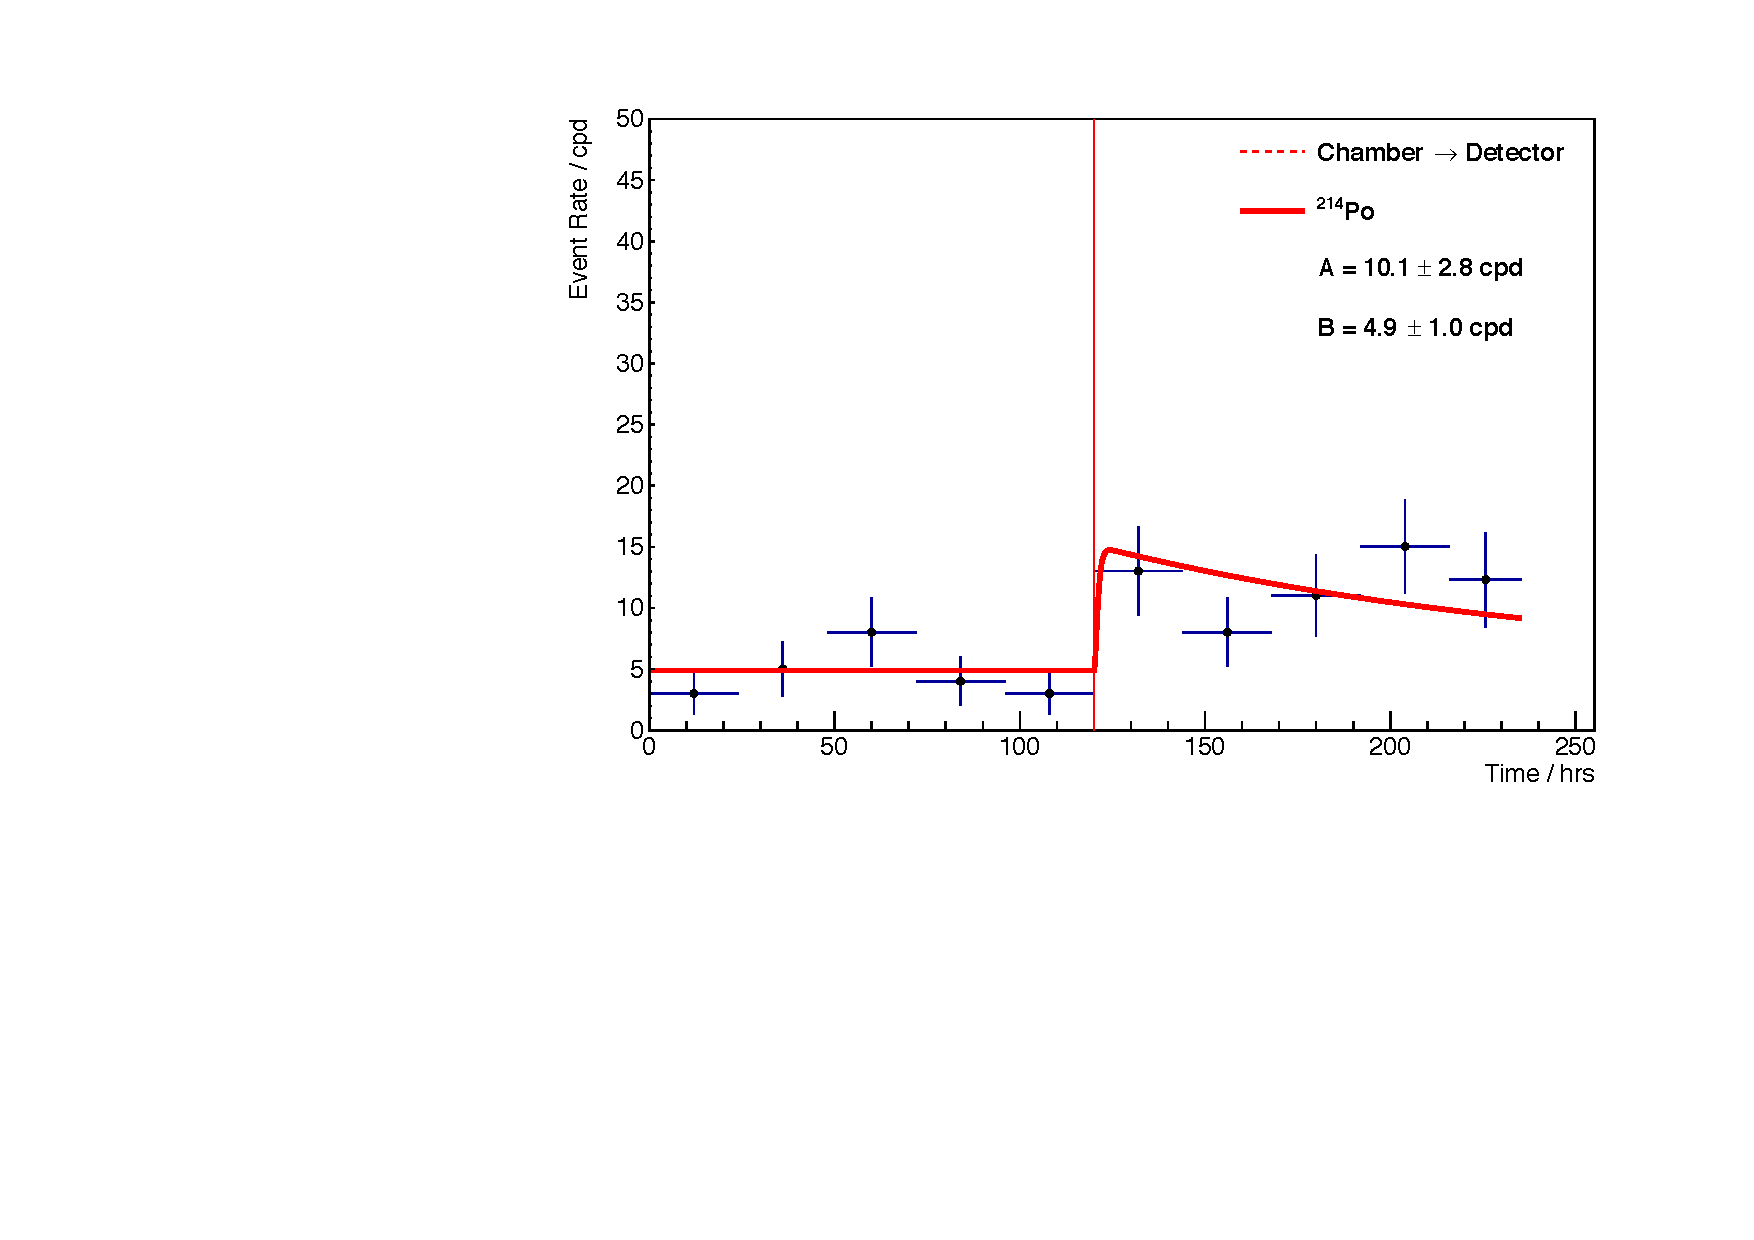
\includegraphics[scale=0.42]{Chapter_4/Figures/ucl_measurements/titanium_welding_block_post_etching_1_Po214.pdf}
    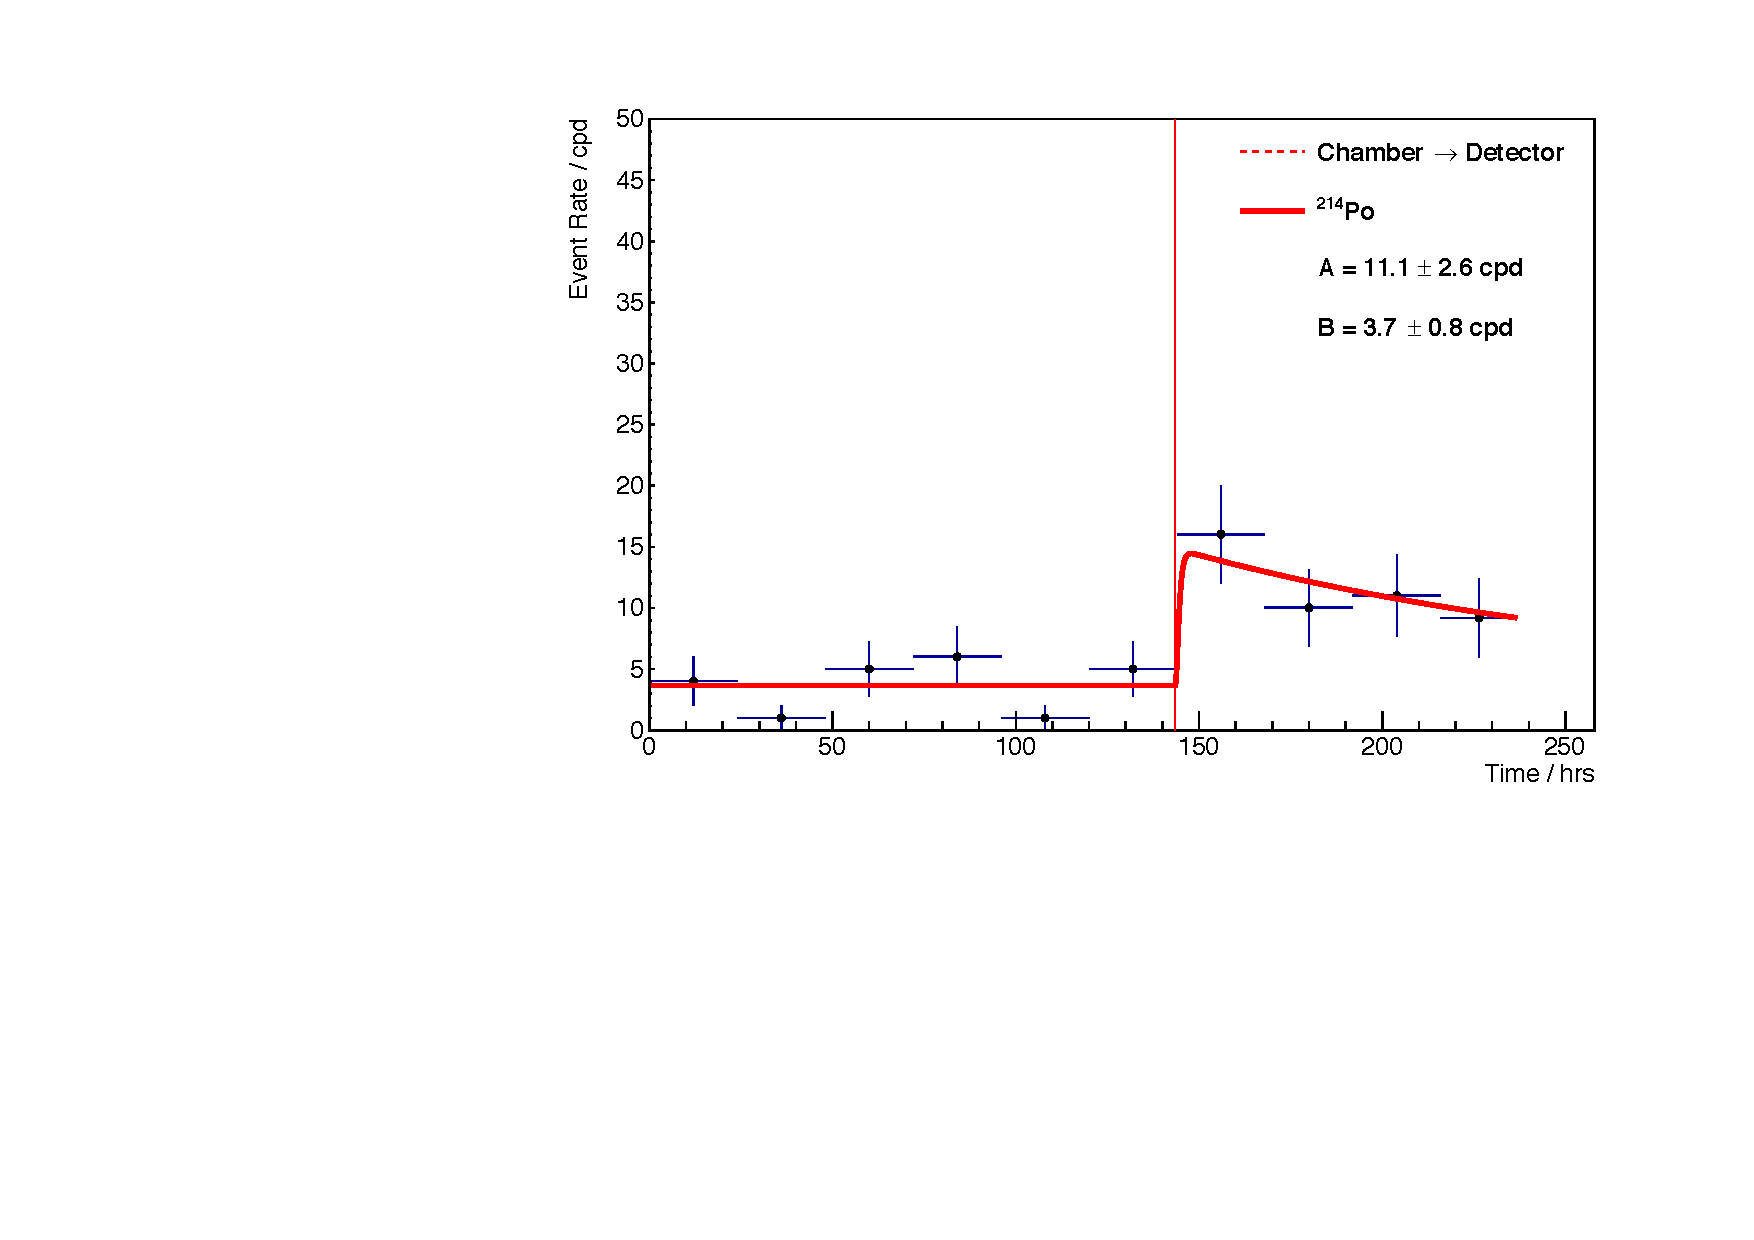
\includegraphics[scale=0.42]{Chapter_4/Figures/ucl_measurements/titanium_welding_block_post_etching_2_Po214.pdf}
    \caption[Pre-corrected \PoTOF{} event rate results obtained from the two measurements made on the post-etched titanium welded block.]
    {Pre-corrected \PoTOF{} event rate results obtained from the two measurement made on the post-etched titanium welded block.}
    \label{fig:ti_post_etched_welded_block_results}
\end{figure}
%

The output from the \PoTOF{} rate of the pre-etched welded block indicated an emanation rate of $560\pm97$ \micro{}Bq, which was in good agreement with \PoTOE{} within error. The averaged output from the post-etched block indicated a rate of $370\pm68$ \micro{}Bq. Although the errors are relatively large and the dataset is constrained by so few measurements, the result seems to indicate that there is a substantial amount of radon emanating out of the block. 


\subsubsection{Titanium Sheets}

To examine radon emanation from the cryostat titanium, a collection of titanium cutouts from the OCV were assayed. 8 pieces totalling to an area of 2350 cm\squared{} were initially wiped down with cleanroom wipes and ultrasonic bathed to remove any dust residue. These sheets are identical to those used in the ICV. Two sets of measurements were performed on the sheets: pre-etched and post-etched measurements. The slight curvature on the sheets, as shown on figure \ref{fig:titanium_welding_sheets}, prevented the sheets from stacking over one another, as stacking could in theory reduce the measured emanation rate due to recoiling atoms lodging into close surfaces. Results obtained for the pre-etched and post-etched sheets are shown in figure \ref{fig:ti_pre_etched_sheets_results} and \ref{fig:ti_post_etched_sheets_results}, respectively. Pre-etched block was measured once, whereas the post-etched block was measured three times.
%
\begin{figure}[b!]
    \centering
    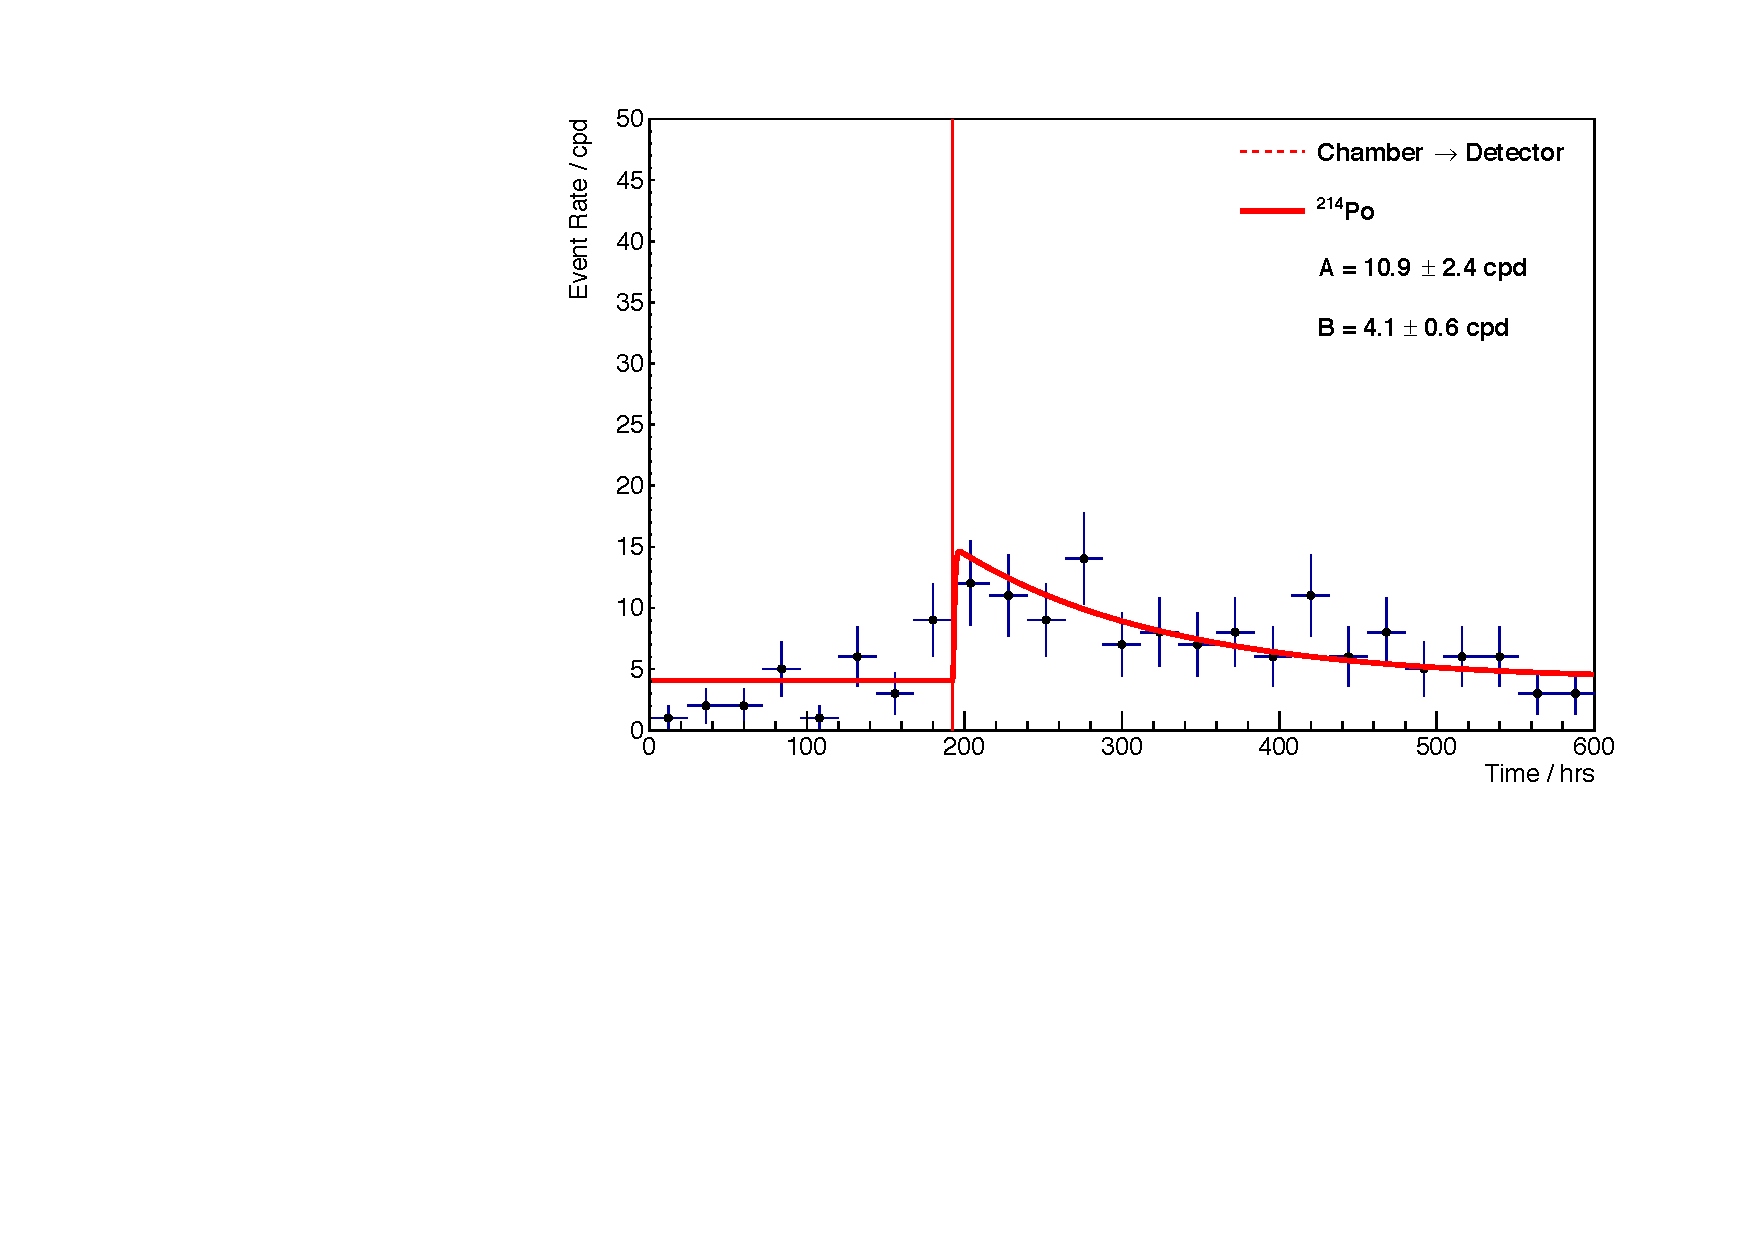
\includegraphics[scale=0.42]{Chapter_4/Figures/ucl_measurements/titanium_sheets_pre_etching_1_Po214.pdf}
    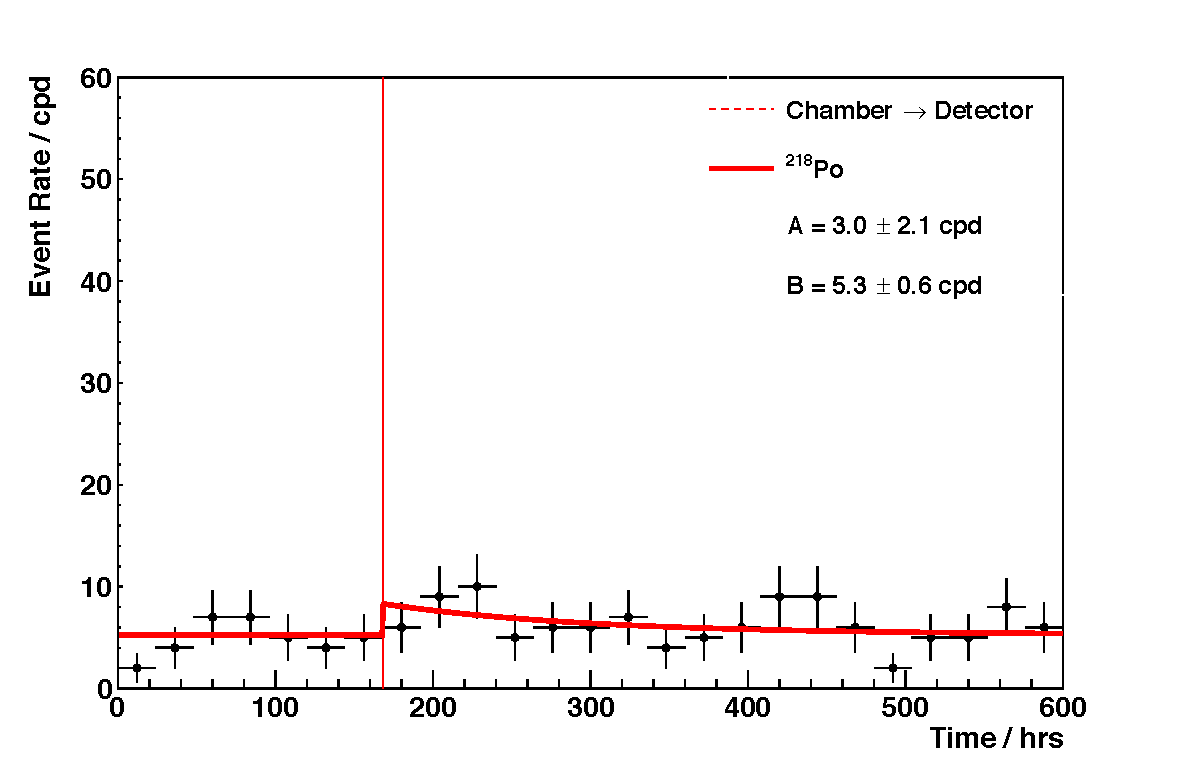
\includegraphics[scale=0.42]{Chapter_4/Figures/ucl_measurements/titanium_sheets_pre_etching_1_Po218.pdf}
    \caption[Pre-corrected \PoTOF{} and \PoTOE{} event rate results obtained from the single measurement made on the pre-etched titanium welded block.]
    {Pre-corrected \PoTOF{} and \PoTOE{} event rate results obtained from the single measurement made on the pre-etched titanium welded block.}
    \label{fig:ti_pre_etched_sheets_results}
\end{figure}
%

The output from the \PoTOF{} rate indicates an emanation rate above the background measured prior to transfer, corresponding to a corrected activity of $380\pm88$ \micro{}Bq. However, the \PoTOE{} rate suggests a background only measurement. This behaviour has previously been observed and is attributed to outgassing of porous samples, for example the \PoTOE{} in comparison to \PoTOF{} has been shown to be suppressed under the presence of (N$_{2}$O). Although a signal has been observed, the presence of neutralising agents may add a systematic error that is currently difficult to determine. 
%
\begin{figure}[t!]
    \centering
    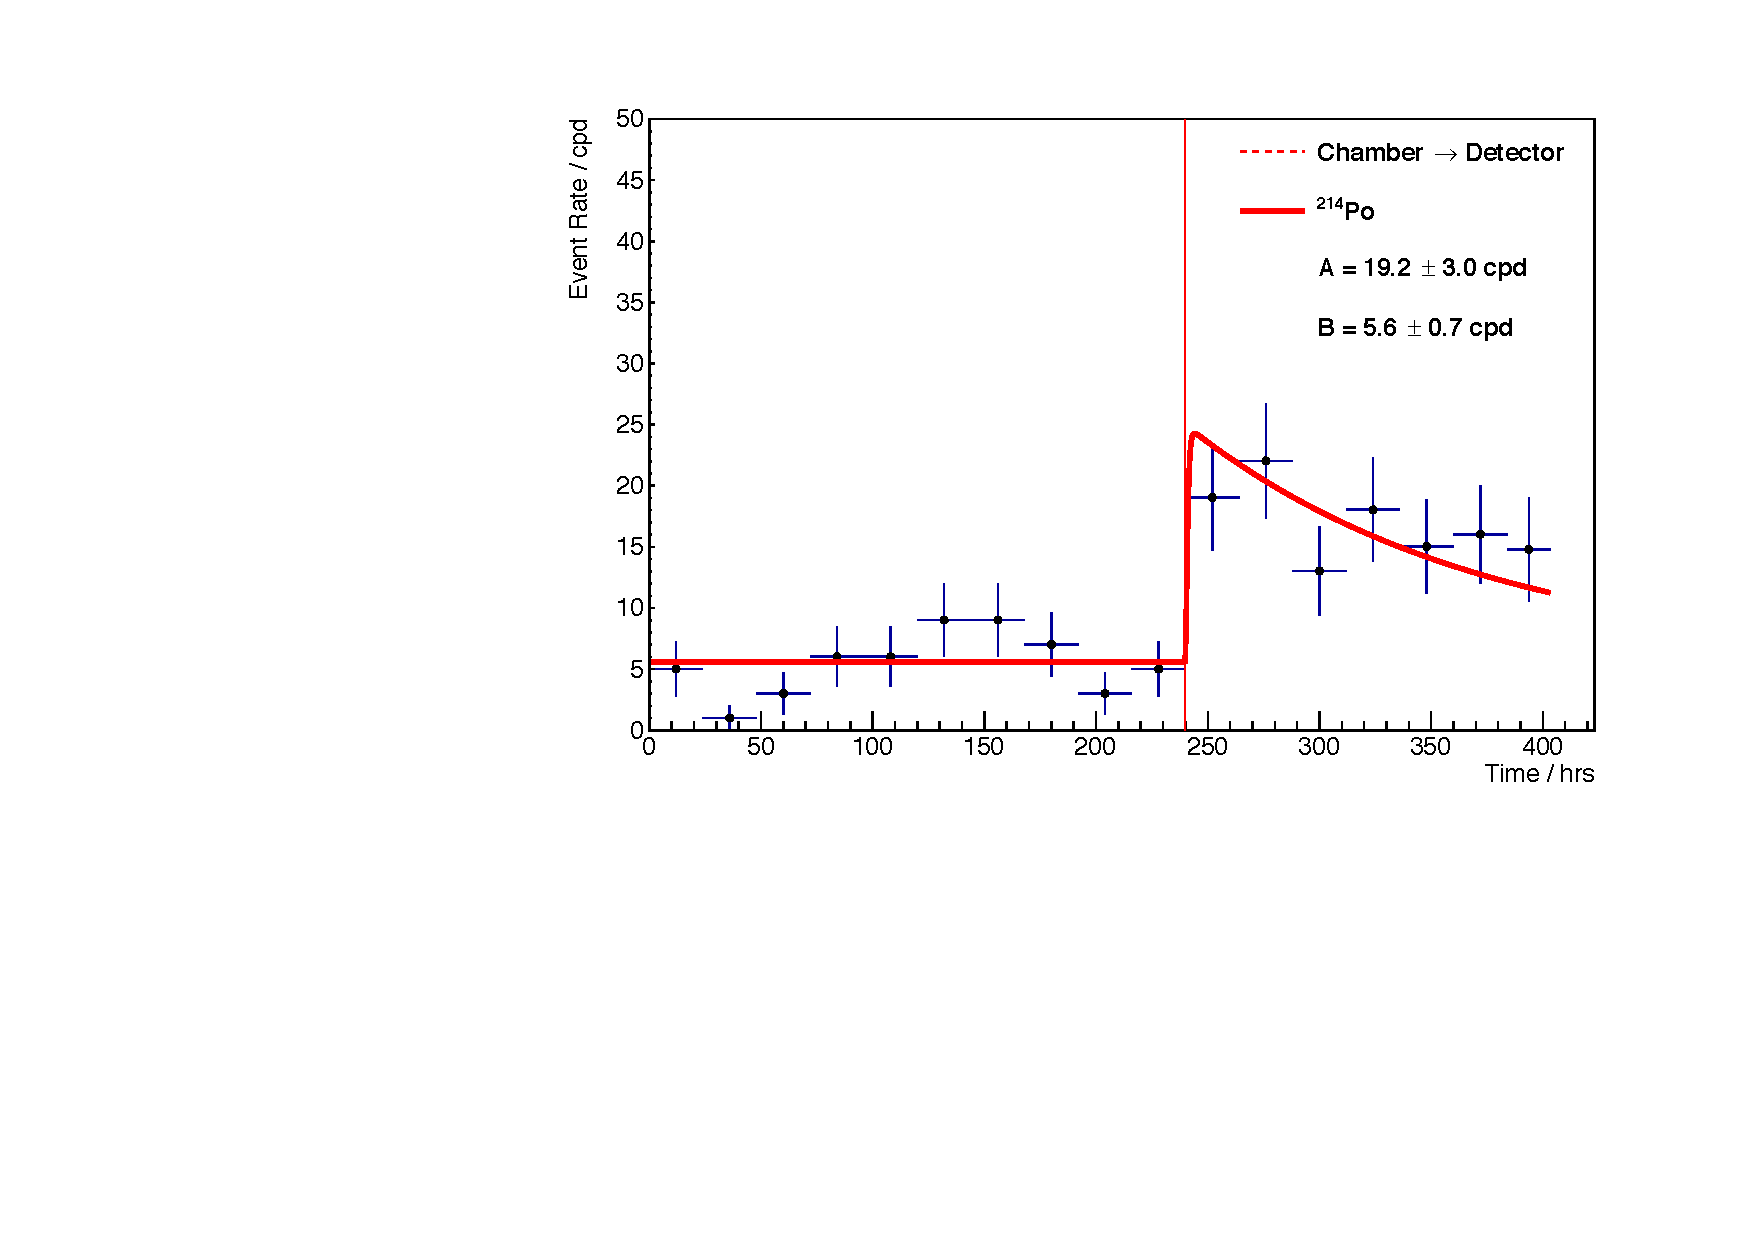
\includegraphics[scale=0.42]{Chapter_4/Figures/ucl_measurements/titanium_sheets_post_etching_1_Po214.pdf}
    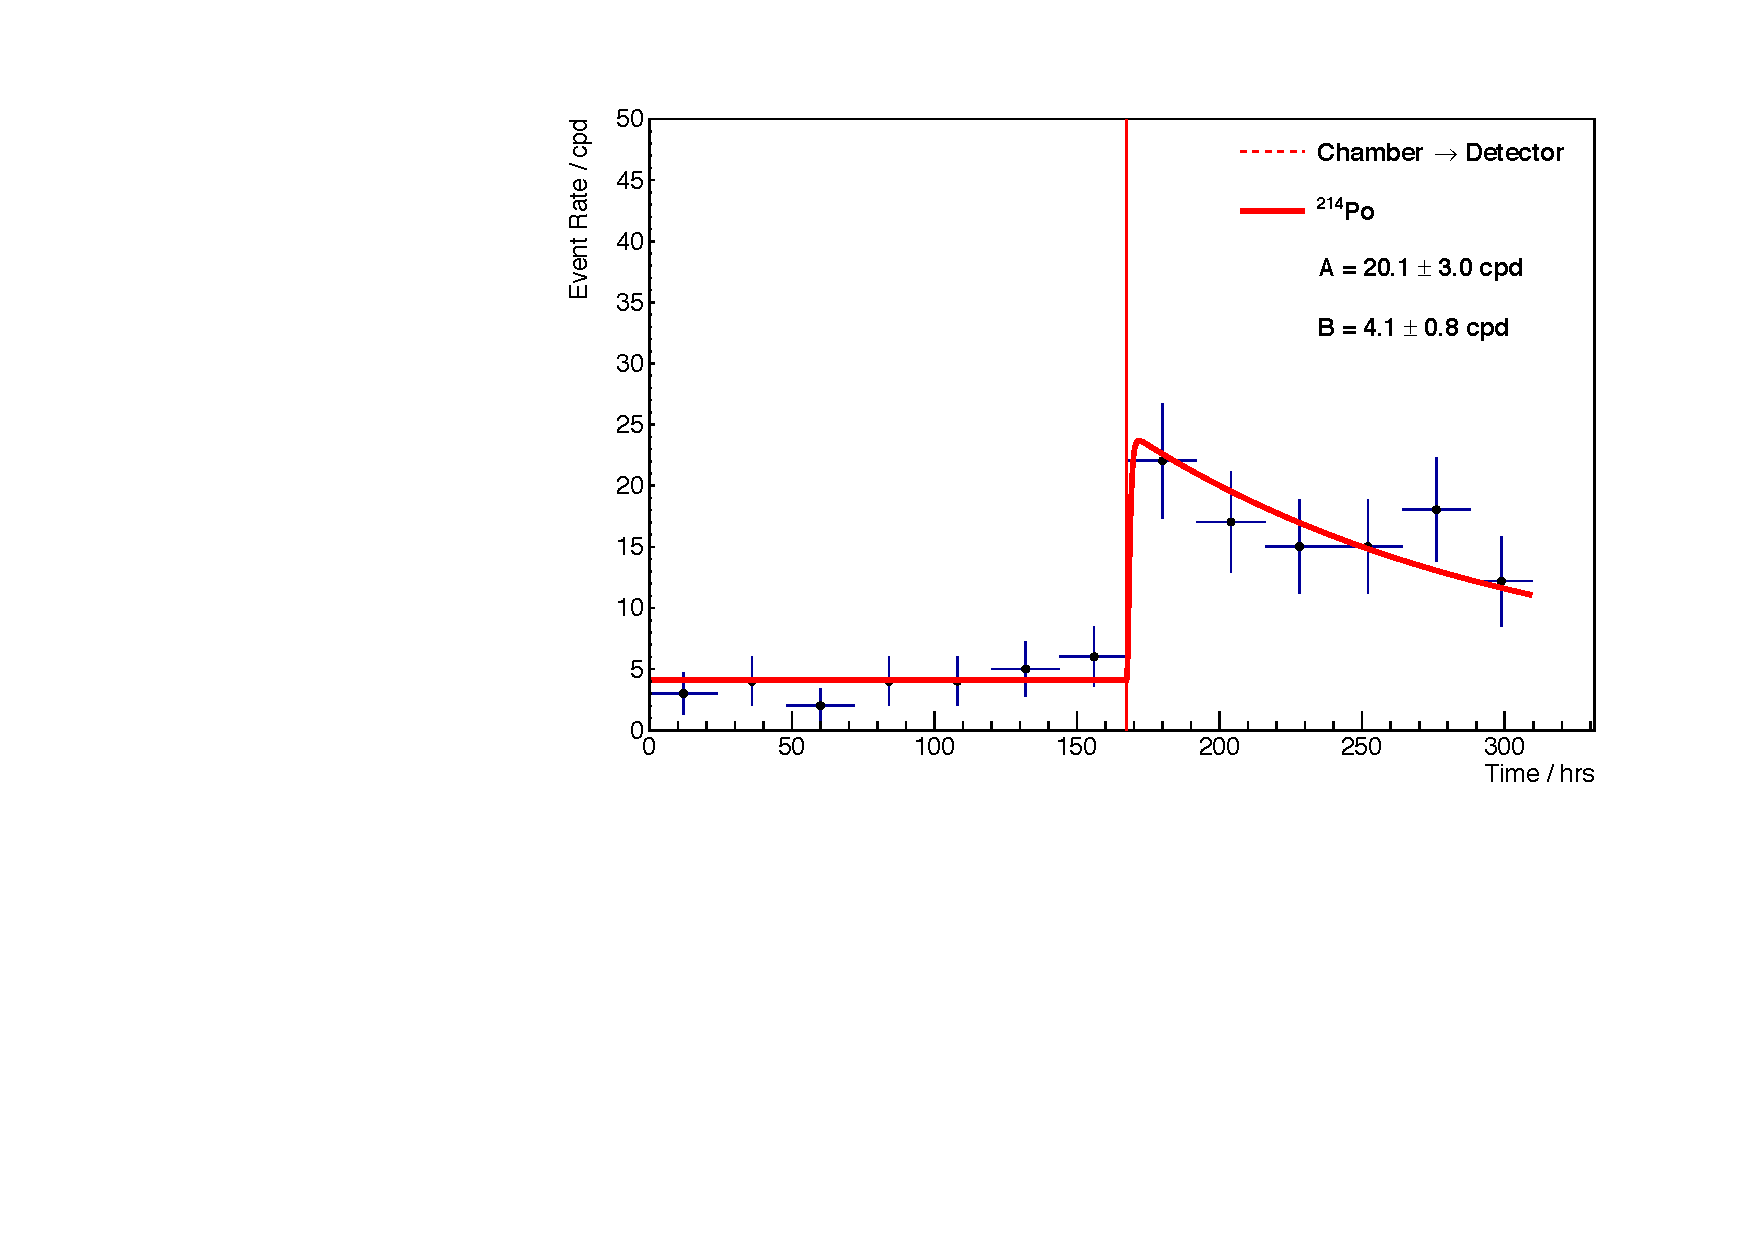
\includegraphics[scale=0.42]{Chapter_4/Figures/ucl_measurements/titanium_sheets_post_etching_2_Po214.pdf}    
    \caption[Pre-corrected \PoTOF{} and \PoTOE{} event rate results obtained from the single measurement made on the pre-etched titanium sheets.]
    {Pre-corrected \PoTOF{} event rate results obtained from the two measurements made on the post-etched titanium sheets.}
    \label{fig:ti_post_etched_sheets_results}
\end{figure}
%

The \PoTOF{} activity measured from the same sample after etching at AstroPak has also shown a signal above the measured background. The two measurements are in good agreement and the averaged rate is calculated to be $685\pm81$ \micro{}Bq. The averaged observed for \PoTOE{} for these two measurements were $476\pm79$ \micro{}Bq. Although there was a clear signal above background, the suppression in comparison to \PoTOF{} still indicates an outgassing induced neutralisation. 

\subsubsection{Discussion \& Conclusion}

The pre- and post-etched emanation rates from the titanium welded block normalised for surface area result in $17.2\pm3.0$ \mBqms and $11.4\pm2.1$ \mBqms, respectively. The surface area normalisation for the titanium sheets for pre- and post-etched measurements give $1.62\pm0.37$ \mBqms and $2.91\pm0.35$ \mBqms, respectively. The titanium results obtained from this study, and for comparison, similar results obtained for stainless steel are highlighted in table \ref{tab:titanium_results}.

The findings from these measurements are unexpected and surprising. The initial expectation for emanation from the titanium was in the order of that measured for stainless steel, but despite the etching, the titanium results in an activity that is $\sim3$ orders of magnitude higher. A small reduction in activity is observed on the titanium welding post etching, but this effect is reversed for the raw titanium sheets, were the activity rises; thus suggesting an ineffectiveness of the etching process on metallic surfaces. Recent results published by the XENON1T collaboration also seem to indicate relatively high emanation rates for titanium. The untreated titanium sheets measured by XENON1T (supplied from Nitronit) are in good agreement with the emanation rates measured for the LZ titanium \cite{Aprile:2020vmn}. They however demonstrate that electropolishing of the titanium surface and removing $\sim30$ $\micro$m from the surface, eliminates all of the measured activity, indicating that the emanation rate is predominantly due to a form of surface contamination. Although electropolishing is known to be a very effective way of removing surface contamination, the size of the LZ detector restricted the use of this technique---leading to alternative forms of etching. 

The total titanium surface within the ICV is 15.1 m\squared{} and a further 0.66 m\squared{} of titanium welding is present in multiple locations. Scaling the etched results from this study to the ICV results in a total emanation rate of $43.9\pm5.3$ mBq and $7.5\pm1.4$ mBq at room temperature for the raw titanium and welded surfaces respectively. For comparison, the bottom-up radon emanation projection prior to the titanium measurement was $\sim20$ mBq from the entire detector. Applying the cross-calibration correction of the UCL detector results in $28.7\pm3.5$ mBq and $4.9\pm0.9$.
%
\begin{table}[h!]
\centering
\caption
[Radon emanation results as obtained from the UCL system for the titanium welded block and titanium sheet assays.]
{Radon emanation results as obtained from the UCL system for the titanium welded block and titanium sheet assays. The results do not take into account the cross-calibration systematic of the UCL detector. For comparison, radon emanation results of titanium (middle rows) and stainless steel welding and foil (bottom rows) are provided, as measured by the XENON1T$^{1}$ collaborations \cite{Aprile:2020vmn} and the GERDA$^{2}$ \cite{osti_20719228, ZUZEL2009889}, respectively.}
\label{tab:titanium_results}
\vspace{1mm}
\renewcommand{\arraystretch}{1.2}
    \begin{tabularx}{1\linewidth}{@{\extracolsep{\fill}}lll}
    \toprule
    
    \textbf{Sample Description} & %1
    \textbf{\RnTTT{} emanation rate} & %2
    \textbf{} & %3
    
    \hline
    \hline
    Titanium welded block (untreated) & $17.2\pm3.0$  & \mBqms{} \\
    Titanium welded block (etched)      & $11.4\pm2.1$  & \mBqms{} \\
    Titanium sheets (untreated)       & $1.62\pm0.37$ & \mBqms{} \\
    Titanium sheets (etched)            & $2.91\pm0.35$ & \mBqms{} \\    

    \hline
    Titanium sheets$^{1}$ (untreated)       & $2.81\pm0.19$ & \mBqms{} \\
    Titanium sheets$^{1}$ (electropolished)       & $<80$ & \uBqms \\
    
    \hline
    Steel welds$^{2}$ (untreated)                   & $0.24\pm0.03$ & \mBqms{} \\   
    Steel welds$^{2}$ (etched \& passivated)          & < 0.1         & \mBqms{} \\
    Stainless steel foil$^{2}$ (untreated)          & $10.2\pm0.8$  & \uBqms{} \\
    Stainless steel foil$^{2}$ (etched \& passivated) & $4.6\pm0.9$   & \uBqms{} \\
    \bottomrule
    \end{tabularx}
\end{table}
%


\subsection{Other Measurements}
\label{secsec:other_emanation}

The UCL radon facility has been used to assay several other components for the LZ experiment. The procedure followed for these assays are identical to those detailed in the former sections. Samples are initially cleaned by cleanroom approved wet wipes prior to the placement into the emanation chamber and left to emanate for $\sim2$ weeks. One week of background data is recorded prior to each transfer and the background rate is subtracted from any observed signal. Results from these measurements are summarised in table \ref{tab:ucl_emanation_results}.

\subsubsection{Cirlex PCBs}

The Cirlex boards screened here are from the same batch of material to those assayed in section \ref{secsec:pmt_base_emanation}, but without all of the electronic components highlighted in table \ref{tab:pmt_base_components}. In an effort to distinguish the radon emanating out of the Cirlex alone a total of 124 3" and 7 1" PCBs, totalling 421 grams were assayed twice. The averaged rate was determined to be $636\pm77$ \micro{}Bq, equating to $1.51\pm0.18$ \micro{}Bq/g. 

\subsubsection{HV Components}

A mixture of HV components were assayed at UCL including; 90" peek rods, 4.5 feet polyethylene tubes, 18 polyethylene displacer discs, 9 feet of fluorinated ethylene propylene (FEP) and 54 polyethylene insulating boomerangs, each provided at a quantity 1.5 times more than required by the LZ detector. Although the activity of the individual components cannot be quantified, an emanation rate of $369\pm85$ \micro{}Bq were measured for the entire batch. 

\subsubsection{DB25s}

As part of the radon screening campaign for the excess ICV radon, a pair of DB25s were assayed. These items were temporarily used in the ICV during the skin installation and hence was an unaccounted item. The measurements resulted in an upper limit of <0.13 mBq.

\subsubsection{Nitrile O-rings}

A total of 90 nitrile rubber o-rings were assayed. The total surface area of the assayed rings were 9.15 cm\squared{}. An emanation rate of $17.6\pm1.7$ mBq was measured per ring. LZ will use a total of 2 nitrile rubber o-rings. 

\subsubsection{Polyoxymethylene (Delrin) Discs}

A collection of 50 Delrin discs with a total surface area of 0.54 m\squared{} was assayed for radon emanation. An emanation rate of $450\pm11$ \uBqms was measured. LZ requires a total of 200 cm\squared{} as part of the installation of the HV umbilical cord, resulting in a contribution of $9\pm2$ \micro{}Bq.


\subsubsection{Titanium Rods}

As part of the radon emanation cross-calibration campaign of the four facilities used by LZ, a set of titanium rods were procured and screened at the various facilitates. A total of 20 rods, 16 cm in lenth and 1 mm in diameter were screened along two small aluminium plates used for structural support. The emanation rate for the sample was measured at $404\pm98$ \micro{}Bq. 


\subsubsection{Summary of Emanation Results}

A summary table of the key measurements made by the UCL system are provided in table \ref{tab:ucl_emanation_results}. The results are provided in easily scalable units for future use and multiple measurements are combined to a single emanation rate. 
%
\begin{table}[h!]
\centering
\caption{Radon emanation results as obtained from the UCL system for all the components measured for the LZ experiment. These results do not include the cross-calibration correction ratio of 1.53.}
\label{tab:ucl_emanation_results}
\vspace{1mm}
\renewcommand{\arraystretch}{1.2}
    \begin{tabularx}{1\linewidth}{@{\extracolsep{\fill}}lll}
    \toprule
    \textbf{Sample Description} & %1
    \textbf{\RnTTT{} emanation rate} & %2
    \textbf{} & %3
    \hline
    \hline
    Titanium welded block (not treated) & $17.2\pm3.0$  & \mBqms{} \\
    Titanium welded block (etched)      & $11.4\pm2.1$  & \mBqms{} \\
    Titanium sheets (not treated)       & $1.62\pm0.37$ & \mBqms{} \\
    Titanium sheets (etched)            & $2.91\pm0.35$ & \mBqms{} \\  
    1" PMT Bases                        & $4.42\pm0.90$ & \micro{}Bq/base \\ 
    3" PMT Bases                        & $5.33\pm0.63$ & \micro{}Bq/base \\ 
    Cirlex PCBs                         & $1.51\pm0.18$ & \micro{}Bq/g \\ 
    HV Components                       & $369\pm85$    & \micro{}Bq/batch \\ 
    DB25s                               & $<0.13$    & \micro{}Bq/unit \\ 
    O-rings (Nitrile)                   & $17.6\pm1.7$    & \micro{}Bq/ring \\ 
    Polyoxymethylene (Delrin) Discs     & $450\pm11$    & \uBqms{} \\ 
    Titanium Rods ($\times$20, L=16 cm, D=1 mm)    & $404\pm98$    & \micro{}Bq \\ 
    \bottomrule
    \end{tabularx}
\end{table}
%


\subsection{Large Scale Radon Emanation Studies}
\label{secsec:large_scale_measurements}

Room temperature measurements from individual material and components measured by various radon facilities are all presented in \cite{lz_screening}. Furthermore, measurements from fully assembled sub-systems, such as the ICV, xenon purification and circulation system are also presented in figure \ref{LZ_radon_diagram_paper}. Measurements for three of these assemblies are discussed in the following sub-sections. These measurements were made possible by the portable radon harvesting system deployed at SURF. 

\subsubsection{Inner Cryostat Vessel}

Radon emanation from the ICV was measured several times during various integration stages of the construction of the skin veto region and the TPC installation. The final assay was made following after the ICV was fully complete and sealed. The cryostat at this stage housed both the top and the bottom PMT arrays for the TPC and the skin veto regions, and their corresponding PMT bases and cables. Furthermore, the entire field cage, PTFE coating, various sensors, and conduit volumes of the cables were a part of these measurement.

A portable radon trapping system was deployed underground at SURF with minimal plumbing due to space constraints. After leak-checking and purging, the trapping system was opened to the ICV and the emanated gas was harvested over a 6.3 hour period---equivalent to 18.25\% of the gas within the ICV. After the harvest, the trap was carefully disconnected and transported to SDSM\&T radon facility for screening. The radon trap also captures outgassing molecular species that would serve as neutralisers of positively charged radon-daughters, leading to a drop in detection efficiency. An in-house procedure was followed to separate out these species by transferring the sample from a cold trap held at -109$^{\circ{}}$C to one at -196$^{\circ{}}$C with sufficient flow to effectively transfer all of the radon atoms while leaving most of the contaminants behind. This process was repeated until measurements with a residual gas analyzer indicated no further reduction in contaminant concentration, after which the sample was transferred to the detection chamber via a secondary small cold trap. Results indicate a room-temperature emanation rate of $46.1^{+4.0}_{-3.8}\,$mBq under the assumption of an even sampling of the radon within the ICV.


\subsubsection{Xenon Circulation System}

The xenon gas circulation system brings together multiple components and surfaces that are potential radon emitters. The system consists of two gas compressors, a heated zirconium getter, and a main valve and instrumentation panel. The compressors (model A2-5/15 from Fluitron) have two heads, each enclosing a flexible all-metal diaphragm sealed with copper plating. Check valves, accumulation bottles, and associated plumbing and instrumentation are also included in the compressor assemblies. The compressors operate in parallel to achieve a gas flow rate of 500 standard liters per minute. Much of the system was fabricated at the University of Wisconsin's Physical Sciences Laboratory. Whilst there, a portable radon trapping system was used to harvest emanation samples that were then shipped to shipped to the U. Maryland radon facility for counting.

Initial radon emanation measurements of compressor 2 found that the heads emanated \SI{< 1}{\milli\becquerel} each, however, the integrated compressor skid assembly presented $\sim$\SI{17}{\milli\becquerel}. After replacing most of the welded stainless steel plumbing and etching the accumulation bottles in citric acid, the rate was reduced to $1.48\pm0.31$\,mBq. A similar treatment was applied to compressor 1 but this compressor was not measured for radon emanation and hence is assumed to have the same rate as compressor 2. The main circulation panel contains most of the valves and instrumentation exposed to the xenon in gas phase, and it was found to contribute \SI{0.74}{\milli\becquerel} of radon. The fully loaded getter (model PS5-MGT50-R-535 from SAES) was measured at its operational temperature of $400 ^{\circ}$C using helium carrier gas and its emanation rate was determined to be \SI{2.26}{\milli\becquerel}. The entire circulation system amounted to a total emanation rate of $5.22\pm0.75$\,mBq.


\subsubsection{Xenon Tower}

The xenon tower is a cryogenic system that thermally couples the gaseous and LXe portions of the purification circuit for efficient heat transfer, serving to vaporize and re-condense the liquid for continuous purification. It consists of a two-phase heat exchanger (supplied from Standard Xchange), three cryogenic valves (manufactured by WAKE), a sub-cooler/phase-separator vessel to hold LXe returning to the detector, a reservoir vessel to hold liquid exiting the detector, two liquid xenon purity monitors, and several custom liquid xenon heat exchangers. The tower can be viewed as having two sides: the heat exchanger assembly on one side and the weir reservoir, sub-cooler and purity monitor on the other. Radon emanation from sub-components was measured prior to full integration of the xenon tower and was found to contribute a total of \SI{<1}{\milli\becquerel}. 

A preliminary measurement of the tower after integration found a very high radon activity in the reservoir side, possibly due to a leak into the system from laboratory air. As a precautionary measure, the reservoir vessel was flushed with a concentrated solution designed for removing radioactive contamination (Radiacwash\textsuperscript{TM}) and rinsed with deionized water. The portable radon trap was then deployed underground to measure the two sides of the complete xenon tower prior to the installation of the purity monitor and found a total emanation rate of $3.14^{+0.86}_{-0.81}$\,mBq.


%%------------------------------$$
\section{Radon Emanation Projection in LZ}
\label{sec:lzradon}
%%------------------------------$$

Sensitivity projections for LZ presented in \cite{akerib2018projected} include the effect of the online charcoal-based radon-removal system, operating continuously to scrub gaseous Xe \cite{lz_tdr, Pushkin:2018wdl}. Although this system will not scrub majority of the xenon within the ICV, a volumetric gas flow of 2 slpm has been shown to eliminate 90\% of the radon from cables and feedthroughs. LZ will utilise on a 7.0 kg charcoal trap to reduce radon emanation from instrumentation immersed in GXe; particularly, radon emanation from the top PMT array, cabling and sensors, along with all the titanium surfaces on the upper-side of the ICV. 

Projections also assume an expected suppression of radon diffusion in certain materials at low temperatures, namely those suspended within the LXe were the operational temperature is 175.8 K (-97.4$^{\circ{}}$C). Its important to note that the radon emanation assays from all the samples---whether individual components screened using emanation chambers, or system-wide instrumentation's screened using a portable harvesting system---were all performed at room temperature (\sim{}20$^{\circ{}}$C).

The projection of radon emanation from warm measurements to operational conditions is a difficult task involving multiple assumptions and approaches. In calculating an operational rate, both the radon reduction system and the suppression due to cold temperature has to be taken into account. The ratio of components sitting within the operational volume of the radon reduction system is well known, but there are still many uncertainties on the suppression rates obtained at cold temperature. Furthermore, these rates heavily depend on the type of material used; more emanation reduction is expected from porous materials like plastics and ceramics when cold. The sections below will initially construct a warm emanation rate projection of the entire detector, and a further attempt to quantify operational rates through literature-based educated assumptions on suppression.  


\subsection{Bottom-up Projection}

Prior to large scale emanation results during construction, the radon projection was constructed entirely from a bottom-up approach from measuring components and material in fractional quantities and scaling the emanation results to quantities present in LZ. The results from this approach with various projections are detailed in table \ref{tab:lz_bottom_up_results}.

Although the table does not fully account for all of the items to be used in LZ, majority of the radon contributors are included. Components such as sensors and screws have previously been emanated but contribute negligible amounts to the total sum. The results obtained by UCL, i.e., the raw titanium, titanium welding and PMT base results, take into account the systematic correction of 0.65 from cross-calibrations. Components that are within the operational ground of the radon removal system are further suppressed by the previously determined 90\% removal efficiency. The GXe suppression factor therefore is $S=0.1$, where the LXe suppression factors are component specific: $S1=0.5,\;S2=0.1,\;S3=0.01,\;S4=0.001,\;S5=0.0001$. The cold reduction values for plastics (S3, S4, S5) originate from diffusivity data on Kapton, Acrylic and PTFE; where temperature dependence of diffusivities of Ar and Kr were evaluated from \cite{Schowalter_2010} by the EXO collaboration and a model for radon is constructed. Components using mixtures of material---such as the bases---use a conservative suppression value ($S2$); though its important to note that the majority of the emanation is from Cirlex ($\rho{}\simeq{}1.42$g/cm$^{3}$), which has a similar density as PTFE ($\rho{}\simeq{}2.2$g/cm$^{3}$). 

Finally, ($S1$) is used for components with metallic surfaces; i.e. PMTs, but more importantly the titanium welding and cryostat. Material such as glass and metals are crystalline in nature and hence space for additional atoms is often limited, especially for the large radon atom. Hence diffusion through such material is suppressed as a nature of the material, as radon would then have to displace or significantly deform the lattice structure to squeeze through, which is heavily suppressed at room temperature. In such a case, emanation is dominated by recoil and hence no suppression at colder temperatures. However, this assumption only applies to perfect lattice structure. The lattice formation depends heavily on the cooling methods when forming the solid metal. A slow cooling process can lead to large crystalline grain formations, whereas a fast cooling process leads to small grains. The grain boundaries represent a surface of imperfect lattice that could be a route for radon to diffuse. 

The expected radon emanation from the LZ detector that emanates directly into volumes in line with the GXe and LXe without any suppression factors result in a rate of $60.8^{6.0}_{-6.1} \;  \MathText{mBq}$. Although not detailed in table \ref{tab:lz_bottom_up_results}, by taking only into account the suppression from the radon removal system and omitting any cold suppression, an emanation rate of $41.3^{+4.4}_{-4.5}$ mBq is obtained. Taking into account the conservative cold suppression factors in table \ref{tab:lz_bottom_up_results}, this rate further drops to $21.6^{+2.3}_{-2.3}$ mBq. If a substantial amount of emanation from the cryostat and the welding is as a result of diffusion, a significant suppression due to cold could be expected. To reflect this, the conservative ($S1$) suppression factor was substituted with ($S2$), giving a total expected emanation rate of $11.0^{+1.0}_{-1.0}$ mBq for an optimistic scenario. The LZ detector is expected to take commissioning data operating fully in GXe and with LXe, hence the comparison of that data to estimations presented here is of utmost interest.

\subsection{Large Scale Assay Projections}

A second method to estimate for the total radon in LZ was by using the large scale measurements highlighted in section \ref{secsec:large_scale_measurements}. Results obtained using this method for the sub-systems of interest is provided in figure \ref{LZ_radon_diagram_paper}. The main difference here is that the entire ICV and the xenon tower has been emanated after the installation of all sub-components. The comparison between large-scale and bottom-up ICV measurements obtained from table \ref{tab:lz_bottom_up_results}, result in a remarkably good agreement, with $46.1^{+4.0}_{-3.8}$ mBq and $48.5^{+5.9}_{-6.0}$ mBq, respectively. Combining the outcomes of the large-scale measurements result in a total emanation rate of $60.4^{+4.2}_{-4.0}$ mBq for the LZ experiment, which in good agreement with the bottom-up estimations when excluding suppression factors.


\subsection{Discussion}
\label{secsec:radon_discussion}

The results obtained from bottom-up assays and large scale emanation measurements during sub-system installation at the SAL are in good agreement within error. A large proportion of the emanation rate is expected from the ICV, of which, the largest contribution comes from the cryostat, welding and the PMT-base pairings. The emanation rate measured from the cryostat titanium was unexpected. Exclusion of the titanium emanation rate from the bottom-up ICV results lead to a substantial underestimation of the emanation rate when compared to the large-scale ICV result. Furthermore, the issue around the UCL systematic adds another layer of complexity, but it is safe to say that this factor is indeed a systematic and not a result of external circumstances. This conclusion is reached when considering the comparison between the ICV bottom-up and total; if this correction was not applied, the bottom-up scenario will substantially overestimate the result from the complete ICV emanation. The agreement between the large scale emanation results and that of the bottom-up adds further confidence to the cross-calibration factor used to estimate radon emanation at operational conditions. Assuming the fraction of radon emanation coming from each sub-component is accurate and the suppression factors are conservative; the worst case scenario with only the radon removal suppression yields an emanation rate of $41.3^{+4.4}_{-4.5}$ mBq. This further reduces to $21.6^{+2.3}_{-2.3}$ mBq and $11.0^{+1.0}_{-1.0}$ mBq when less conservative ($S1\rightarrow{}S2$) suppression factors for LXe are successively assumed. Chapter \ref{chap:chap5} will investigate the significance of the radon background for the WIMP search, studying the implications of these scenarios for the sensitivity and the discovery potential of WIMPs.

%
\vspace{1.5cm}
\begin{figure}[h]
    \centering
    \hspace*{-0.2cm}
    \includegraphics[scale=0.3]{Chapter_4/Figures/LZ_Radon_Diagram_Paper.png}
    \caption
    [Approximate schematic of LZ highlighting key sub-systems and xenon circulation paths in and out of the ICV.]
    {Approximate schematic of LZ highlighting key sub-systems and xenon circulation paths in and out of the ICV. The diagram condenses some of the key radon emanation measurements that will contribute to the overall radon budget of LZ. The results presented in green text are directly from measurements and those in black show summed results for that particular component. All of the results shown are measurements made at room temperature and does not include the cold suppression expected under full operation.}
    \label{LZ_radon_diagram_paper}
\end{figure}
%

%
\begin{table}[p!]
\centering
\caption{Results obtained from component and material radon emanation from various facilities used by LZ. The UCL results provided take into account the systematical fraction highlighted in table (\ref{tab:ReDet}). Provided are the components and quantities used in LZ and emanation results obtained from same/similar samples. Fraction of components occupying either the GXe region of the detector---where radon removal system will operate, or the LXe region---where cold suppression is considered. Emanation rates expected from these two regions after applying the suppression factors is given in the last two columns. The  GXe suppression factor is S=0.1, where the LXe suppression factors are component specific: S1=0.5, S2=0.1, S3=0.01, S4=0.001, S5=0.0001. Those components were neither suppression factor apply are left blank; i.e. xenon tower and circulation. The remaining results from the radon emanation campaign are detailed in \cite{lz_screening}.}
\label{tab:lz_bottom_up_results}
\vspace{1mm}
\renewcommand{\arraystretch}{1.2}
    \begin{adjustbox}{width=\textwidth,center}
    \tabcolsep=4pt
        \begin{tabular}{lcc|cc|cc|cc}
        \toprule
        
        \multicolumn{1}{l}{\textbf{Component}} %1
        & \multicolumn{2}{c|}{\textbf{Quantity}} %2
        & \multicolumn{2}{c|}{\textbf{\RnTTT}} %4
        & \multicolumn{2}{c|}{\textbf{Location [\%]}} %6 
        & \multicolumn{2}{c}{\textbf{Suppression [\micro{}Bq]}} \\ %7 
        
            %1
        &   %2
        &   %3
        &   %4
        &   %5
        & GXe %6
        & LXe %7
        & GXe %8
        & LXe \\ %9
        
        \hline
        \hline
        
        \textbf{ICV} &  &  &  &  &  &  &  &  \\
        
        Titanium (Raw)\textsuperscript{S1} & 15.1 & m\squared & 2910.0$^{+0.4}_{-0.4}$ & \uBqms & 0.25 & 0.75 & 35.90 & 10769.85 \\
        Titanium (Welding)\textsuperscript{S1} & 0.66 & m\squared  & 7451.0$^{+2.1}_{-2.1}$ &	\uBqms & 0.10 &	0.90 & 2.46 & 2212.94 \\
        3" PMTs (R11410)\textsuperscript{S1} & 494 & unit & 1.8$^{+1.7}_{-1.8}$ & \micro{}Bq/unit & 0.51 & 0.49 & 2.28 & 216.96 \\
        PMT Bases (3")\textsuperscript{S2} & 499 & unit & 3.5$^{+0.6}_{-0.6}$ & \micro{}Bq/unit & 0.51 & 0.49 & 4.46 &	84.66 \\
        2" PMT (R8520)\textsuperscript{S1} & 48 & unit & 1.8$^{+1.0}_{-1.3}$ & \micro{}Bq/unit & 0.00 & 1.00 & 0.00	& 43.92 \\
        PMT Bases (2")\textsuperscript{S2} & 49 & unit & 3.5$^{+0.6}_{-0.6}$ & \micro{}Bq/unit & 0.00 & 1.00 & 0.00	& 17.07 \\
        1" PMT (R8778) & 93 & unit & 7.1$^{+2.6}_{-3.0}$ & \micro{}Bq/unit & 1.00 & 0.00 & 3.30 & 0.00 \\
        PMT Bases (1")\textsuperscript{S2} & 94 & unit & 2.9$^{+0.9}_{-0.9}$ & \micro{}Bq/unit & 0.99 &	0.01 & 1.34 & 0.30 \\
        Cables (Axon)\textsuperscript{S4} &	14802 &	m &	0.6$^{+0.1}_{-0.1}$ & \micro{}Bq/m & 0.55 &	0.45 & 24.65 &	4.10 \\
        Cables (Koax)\textsuperscript{S4} &	1771 & m & 0.03$^{+0.23}_{-0.03}$ &	\micro{}Bq/m & 0.70 & 0.30 & 0.16 &	0.01 \\
        PTFE\textsuperscript{S5} & 84 &	m\squared & 12.4$^{+5.3}_{-10.0}$ & \uBqms & 0.00 & 1.00 & 0.00	& 0.10 \\
        Kapton Sheets &	1.25 &	m\squared &	56.0$^{+104.0}_{-56.0}$ & \uBqms & 1.00 & 0.00 & 0.35 &	0.00 \\
        HV Feedthrough & 21 & unit & 37.0$^{+12.0}_{-12.0}$ & \micro{}Bq/unit &	1.00 & 0.00 & 3.89 & 0.00 \\
        Signal Feedhrough &	31 & unit &	23.0$^{+18.0}_{-14.0}$ & \micro{}Bq/unit & 1.00 & 0.00 & 3.57 & 0.00 \\
        Anode/Cathode Feedhrough & 3 &	unit &	18.8$^{+19.0}_{-18.8}$ & \micro{}Bq/unit & 1.00 & 0.00 & 0.28 &	0.00 \\

        \hline
        \textbf{HV Umbilical} &  &  &  &  &  &  &  &  \\
        Umbilical Cable\textsuperscript{S3} & 7.8 &	m &	52.0$^{+8.0}_{-8.0}$ & \micro{}Bq/m & 0.51 & 0.49 & 1.04 &	1.98 \\
        Mixed Components\textsuperscript{S2} & 0.67 & batch & 369.0$^{+85.0}_{-85.0}$ & \micro{}Bq/batch & 0.20 & 0.80 & 0.25 & 19.68 \\
    
        \hline
        \textbf{Radon Removal \& Transfer Lines} &  &  &  &  &  &  &  &  \\
        Activated Carbon (Trap) & 6 & kg & 510.0$^{+90.0}_{-90.0}$ & \micro{}Bq/kg & 1.00 &	0.00 & 400.86 & - \\
        Radon Reduction Panel &	1 & unit & 290.0$^{+110.0}_{-110.0}$ & \micro{}Bq/unit & 1.00 &	0.00 & 1.45 & - \\
        Xenon Transfer Lines & 1 & unit	& 220.0$^{+70.0}_{-70.0}$ &	\micro{}Bq/unit & 0.00 & 1.00 & 0.00 & 220.00 \\

        \hline
        \textbf{Xenon Circulation} &  &  &  &  &  &  &  &  \\
        Purification Getter & 1 & unit & 2260.0$^{+280.0}_{-280.0}$ & \micro{}Bq/unit &	- &	- & 2260.00 & - \\
        Compressors & 2 & unit & 1480.0$^{+310.0}_{-310.0}$ & \micro{}Bq/unit & - & - & 2960.00 & - \\
        Circulation Panel &	1 &	unit & 740.0$^{+200.0}_{-200.0}$ & \micro{}Bq/unit & - & - & 740.00 & - \\   
        
        \hline
        \textbf{Xenon Tower	} &  &  &  &  &  &  &  &  \\
        Xylem HEX &	1 & unit & 529.0$^{+132.0}_{-132.0}$ &	\micro{}Bq/unit & - & - & 529.00 & - \\   
        Subcooler HEX &	1 &	unit & 300.0$^{+140.0}_{-300.0}$ & \micro{}Bq/unit & - & - & 300.00 & - \\   
        WEKA Valves & 3 &	unit & 60.0$^{+10.0}_{-10.0}$ &	\micro{}Bq/unit & - & - & 180.00 & - \\   
        Conditioning Heater &	2 &	unit & 36.0$^{+17.0}_{-15.0}$ & \micro{}Bq/unit & - & - & 72.00 & - \\   
        Misc Others & 1 & batch & 500.0$^{+500.0}_{-500.0}$ & \micro{}Bq/batch & - & - & 500.00 & - \\   
        
        \hline
        \hline
        
        \textbf{Sub-total [mBq]} & & & & & & & \textbf{8.03$^{+0.89}_{-0.93}$} & \textbf{13.6$^{+2.1}_{-2.1}$} \\
        \textbf{Total [mBq]} & & & \textbf{60.8$^{+6.0}_{-6.1}$} &  & & & \multicolumn{2}{c}{\textbf{21.6$^{+2.3}_{-2.3}$}} \\
        
        \bottomrule
        \end{tabular}
    \end{adjustbox}
\end{table}
%
  \chapter{LZ Sensitivity Studies}
\label{chap:chap5}

Understanding the physical response of a detector to its environment is key in assessing the capacity of the detector in looking for the desired physics objectives. Furthermore, detector design has to take into account this response to optimise construction and allow for the testing of theories and models by comparison to data. Over the past few years, the LZ simulation and statistical packages were developed alongside the design and construction of the experiment. The focus of this chapter is initially to give a brief introduction to these packages, focusing primarily on the statistical software package \textsc{LZStats}, which has been developed and used to study the sensitivity and discovery potential of the experiment to WIMP dark matter. Moreover, sensitivity studies are presented using the statistical framework, showing how varying levels of radon and other backgrounds in the detector impact our science reach; highlighting the essentiality of precision understanding and reduction of the backgrounds to maximize detector sensitivity.


%%------------------------------$$
\section{Overview}
\label{sec:overview_5}
%%------------------------------$$

The instruments used in pursuit of new physics becomes a playground in which new discoveries can be made. However, without fully understanding the internal dynamics of this playground and the precise response mechanics taking place as a result of known (background) and unknown (signal) interactions, the ability to claim a discovery is diminished. Simulation of detectors through the means of Monte Carlo modeling is an essential tool in physics to test theories and models by comparison to data, and more importantly, to understand the response dynamics of such a playground to these interactions. 

Although the origin of background events and their response mechanisms in LXe are well understood, this alone is not enough to determine the actual rates observed by the entire system operating in unison. The simulation of events for LZ serves multiple purposes; the primary of which is to determine an optimal detector design that takes into account material specific background rates, and their physical and geometric features in constructing an ultra low-background detector optimised for the detection of WIMPs. Furthermore, upon a verified detector design, the simulations are used for the calculation of background rates in LZ with input from radioactivity measurements. Through the use of these rates and by utilising on a Profile Likelihood Ratio analysis (PLR), the sensitivity of the experiment to various rare event searches is predicted. 

The LZ simulation chain brings together a class of packages that simulate the response of the detector beginning from the initial interaction point---the point of first energy deposition, all the way through the electronic and algorithmic response models in creating a realistic event topology. The chain starts with a \textsc{Geant4} based in-house code \textsc{BACCARAT}, standing for 'Basically a component centric analog response to anything', to track the passage of particles through the detector, identifying and recording their interaction points. The output from \textsc{BACCARAT} is further used in two separate chains as detailed in figure \ref{fig:lz_simulation_chains}. 

%
\begin{figure}[b]
    \centering
    \hspace*{-0.2cm}
    \includegraphics[scale=0.7]{Chapter_5/Figures/LZ_simulations_chains.jpg}
    \caption
    [The LZ simulation packages, detailing the fast and the full processing chains of background simulations.]
    {The LZ simulation packages, detailing the fast and the full processing chains of background simulations. The fast chain is primarily used in sensitivity studies, whereas the full chain is used to generate ultra-realistic pulses for Mock Data Challenges (MDCs).}
    \label{fig:lz_simulation_chains}
\end{figure}
%

The fast simulation chain records energy depositions using \textsc{BACCARAT} and passes these depositions over to \textsc{NEST}, where the energy depositions are converted into S1 and S2 signals by using well understood light and charge yields in LXe, and applying detector-averaged quantities. In enabling fast generation of large datasets, this chain is often used in analysing background rates and informing sensitivity estimates. However, more minute details of events, such as, times of interaction and PMT photon hits are inaccessible. The full simulation chain includes the simulation of VUV photons and ionization electrons that are produced during xenon interactions, as well as the scintillation light generated in the skin and OD veto systems. Furthermore, a detector electronics response (DER) simulation is used to model the PMT response to VUV photons including quantum efficiency and dark noise, front-end and back-end electronics to generate realistic waveforms. These waveforms are stored in realistic data structure to that of expected data---facilitating a training dataset used to prepare for real data through Mock Data Challenges (MDCs). These waveforms are passed through the LZ Analysis Package (LZap), which reconstructs pulse and event level information through a multitude of algorithms for data analysis.

The simulation studies highlighted in this chapter focus predominantly on the fast simulation chain. The expected backgrounds from screening results are used as a bases to input into \textsc{BACCARAT}, where detector related background rates are determined. Dedicated particle generators are used to simulate surface and xenon contaminants; backgrounds from the cavern, cosmogenic muons and various physics backgrounds, such as solar, atmospheric and diffused supernova neutrinos. NEST is then used to generate background specific S1 and S2 signals that plug into the \textsc{LZStats} framework for the evaluation of sensitivity projections. The following sections will give a brief introduction to the fast simulation chain used in this work, a more in-depth highlight can be found in \cite{lz_simulations}. A description of \textsc{LZStats} framework and its statistical approach is detailed. Furthermore, projections made for the WIMP sensitivity of the LZ dark matter experiment and various other sensitivity studies, emphasising on the impact of the dominant radon background of LZ are presented.


%%------------------------------$$
\section{LZ Simulation Framework \& Detector Parameters}
\label{sec:LZ_simulation_framework}
%%------------------------------$$


\subsection{BACCARAT}
\label{secsec:BACCARAT}

\textsc{Geant4} is a toolkit used extensively in the nuclear and high-energy physics community to simulate the passage of particles and particle interactions through detectors and materials. The LZ simulation package \textsc{BACCARAT} is an extension to the simulation package developed for LUX \cite{AKERIB201263}, providing a more user-friendly interface to \textsc{Geant4} for low-background experiments. Simulations in low-background experiments differ to conventional particle colliders due to the origin of background sources. In low-background experiments, such as LZ, one of the main sources of background is embedded radioactive isotopes scattered throughout detector material; placing the source of radiation across a three-dimensional volume. Furthermore, every material and component within the detector has a unique radioactive composition; the simulation of which requires a collection of sources with potentially complicated spatial and radioactive extent.

\textsc{BACCARAT} is a simulation framework designed and used by LZ that takes a component-centric approach to event generation and recording. It implements a C++ detector component object that allows for spacial origin for radioactivity across a three-dimensional component or material for a more accurate modeling of impurities. Furthermore, each component can independently have a material specific recording level for the amount of information required, such as position, scattering information or energy deposition---significantly improving memory usage. The defined geometry of the LZ detector, illustrated on figure \ref{fig:lz_geometry_viz} relies heavily on \textsc{Geant4} classes.

%
\begin{figure}[b]
    \centering
    \includegraphics[scale=0.21]{Chapter_5/Figures/lz_geometry_viz.png}
    \caption
    [The geometry of the LZ detector as constructed by the \textsc{BACCARAT} simulation package illustrating some of the key components.]
    {The geometry of the LZ detector as constructed by the \textsc{BACCARAT} simulation package illustrating some of the key components. The entire detector is immersed inside a water tank, with the inner part of the water tank shown in blue; holding the OD PMT structure, which face the GdLS outer detector tanks (yellow). The outer and the inner. cryostat (light green) holds the central TPC (magenta).}
    \label{fig:lz_geometry_viz}
\end{figure}
%

In modeling various physics processes, \textsc{BACCARAT} implements several modules that are contained in the \textsc{Geant4} toolkit, including \textit{G4EMLivermorePhysics}---covering electromagnetic interactions for \gamma{}-rays and electrons down to $\sim10$\,eV, where low energy processes, such as bremsstrahlung, the photoelectric effect, Rayleigh and Compton scattering are modeled \cite{osti_295438, osti_5691165}. Furthermore, when run in full simulation mode, \textsc{BACCARAT} implements a custom-built physics list (NEST) directly into the \textsc{Geant4} interface under \textit{G4S1Light} \& \textit{G4S2Light}, governing the detector specific generation of light and charge quanta in a xenon volume, respectively.

In addition to these, there are several other physics lists that have been implemented to simulate various other potential event topologies in LZ, such as, Cherenkov processes in non-xenon materials, rest and in-flight decay of radioactive nuclei via \alpha, $\beta{}^{\pm}$, \gamma-emission or electron capture; and relaxation of excited atomic states via the emission of X-rays and electrons. The \textsc{BACCARAT} physics list, particle generators and processes such as charge transport within xenon are continually improved for more realistic simulations. The code is maintained via an LZ inclusive Git repository and the studies highlighted in this chapter are with BACCARAT verified against \textsc{Geant4} version 10.3.


\subsection{NEST}
\label{secsec:NEST}

The NEST package introduced in section \ref{subsubsec:light_charge} plays a key role in the fast simulation chain. NEST is a semi-empirical collection of models, relying on data from a multitude of past and present science and calibration datasets for \beta, \gamma and neutron-induced xenon recoils in varying electric fields, simulating the excitation, ionization, recombination, and electron electroluminescence processes in liquid or gaseous xenon. The previous versions of NEST \cite{Szydagis_2011, Mock_2014} modeled light and charge yields as a function of energy inspired by the Thomas-Imel box recombination model at low energies \cite{PhysRevA.36.614} and Doke modification to Birks’ law \cite{DOKE1988291} at high energies, with coefficients as functions of field. The version used as part of this study, v2.0, uses a range of sigmoidal-class functions to model yields as functions of energy \cite{nest_v2}. The yields are readily modeled as a function of particle and interaction type, energy, ionisation density, electric field and fluid density.

The output from \textsc{BACCARAT}; information on energy deposition, material media, type of interaction, is fed into NEST for a rapid conversion into the detector observable quantities. The conversion from deposited energy to detector observables (S1 \& S2) is calculated in multiple steps, where the exciton-to-ion ratio is first considered to determine the amount of excitons, leading to primary scintillation (S1) and electron-ion pairs. Energy-specific recombination probabilities are then applied to determine the amount of electron-ion recombination, resulting in a reduction in S2 signal, but an increase in S1. For processes where energy is lost through heat, i.e., nuclear recoil events, a simple power law approximating the Lindhard factor is applied \cite{Lindhard, Lindhard_2}. The transportation of escaped electrons to the liquid-gas interface is handled by NEST through a parametrised electric field applying diffusion and a finite mean free path; where upon reaching this barrier, an extraction efficiency is applied through probabilistic quantities dependent on extraction field strength in the gas phase. The resulting output from NEST then takes into account detector specific quantities to produce a corrected S1$_{c}$ and S2$_{c}$ signal in \textit{photons detected} (phd).


\subsection{Detector Parameters}
\label{secsec:detector_param}

%
\begin{table}[b!]
\centering
\caption
[Key detector parameters for the LZ experiment.]
{Key detector parameters for the LZ experiment. PDE refers to \textit{photon detection efficiency}, SE to \textit{single electron}, e to \textit{electron}, ph and phd to \textit{photon} and \textit{photons detected}, respectively.}
\label{tab:lz_parameters}
\vspace{1mm}
\renewcommand{\arraystretch}{1.2}
    \begin{tabularx}{0.7\linewidth}{@{\extracolsep{\fill}}lll}
    \toprule
    \textbf{Detector Parameter} & %1
    \textbf{Value} & %2
    \textbf{} & %3
    \hline
    \hline

    Drift electric field                        & 310 & V/cm \\
    Electron lifetime                           & 850 & \micro{}s \\
    Electron extraction efficiency              & 95 & \% \\
    Average PMT efficiency                      & 27 & \% \\
    Average PDE in liquid (\textit{g$_{1}$})    & 0.119 & phd/ph \\
    Average PDE in gas (\textit{g$_{1gas}$})    & 0.102 & phd/ph \\
    Single electron size                        & 83 & phd \\
    Effective charge gain (\textit{g$_{2}$})    & 79.2 & phd/e \\
    S1 coincidence level                        & 3 & ph \\
    Single phe trigger efficiency               & 95 & \% \\
    PTFE reflectivity in LXe                    & 97.7 & \% \\
    PTFE reflectivity in GXe                    & 85 & \% \\ 
    
    \bottomrule
    \end{tabularx}
\end{table}
%

The detector parameters that are key in determining the actual observed signal for \textit{S1, S2, x-y-z}, from the point of interaction and through the physical and electrical processes of LZ are summarised in table \ref{tab:lz_parameters}. Once an event occurs within the LXe volume, the photons that are produced---referred to as raw S1---traverse the volume, reflecting off of the PTFE walls before hitting a PMT successfully. The $g_{1}$ factor, formally known as the photon detection efficiency in the liquid represents the averaged successful recording of a single photon, taking into account reflectively and PMT quantum efficiencies; $g_{1gas}$ is the equivalent detection efficiency for S2 electroluminescence photons generated in the gaseous extraction region. The current estimates derived from optical simulations based on reflectively measurements of the LZ PTFE \cite{Neves_2017, Haefner_2017} for $g_{1}$ and $g_{1gas}$ are 0.119 phd/ph and 0.102 phd/ph, respectively. These values include considerations of 3'' Hamamatsu PMT quantum efficiency, double photoelectron emission probabilities \cite{L_pez_Paredes_2018}, first dynode collection efficiency and photon absorption length in LXe motivated by the literature \cite{lux_signal_yields}. Single electron size represents the average number of photons detected per extracted electron, whereas the photons detected from a raw S2 signal is represented by the $g_{2}$ factor. $g_{2}$ takes into account the extraction efficiency at the liquid-to-gas boundary, adding an averaged correction for the lost electrons, resulting in an effective charge gain of 79.2 phd/e.

The detector parametrisation factors detailed in table \ref{tab:lz_parameters} are evaluated alongside the \textsc{BACCARAT} input to the \textsc{NEST} framework in calculating corrected detector observable signals, S1$_{c}$ and S2$_{c}$. Although this process takes certain parameters as their averaged representations; excluding differences arising from event location, or PMT specific divergences on an event-to-event bases; it allows for fast generation of (S1$_{c}$, S2$_{c}$) probability density functions (PDF) that are representative of detector operational conditions. The PDFs of background and signal events are then fed into the LZ statistical framework, \textsc{LZStats}, for sensitivity studies. The event selection criteria and the representative background rates under projected operational conditions, as determined by the use of the LZ simulation framework are detailed in the next section.   



%%------------------------------$$
\section{Background Projections for WIMPs}
\label{sec:uclradon}
%%------------------------------$$

The LZ detector is capable of detecting signals from a wide spectrum of event topologies and energy ranges. This wide range of energy-space is made accessible by exploiting the two signal types in LZ, measurement of scintillation light and charge production, in various search types; i.e. S2-only, S1-S2 and S1-only searches. At sub-keV energies, S2-only searches are used to probe for lighter WIMPs, sub-GeV hidden sector and asymmetric dark matter models. Low energy depositions at this regime usually result in free electrons extracted without any accompanying S1 signal. At much higher energies, LZ is capable of probing the \XeOTS{} \neutrinolessDoubleBeta{}-decay with a $Q_{\beta \beta}$ value of 2458 keV \cite{Akerib_2020_double_beta}.

The observation of a WIMP signal is conducted in the S1-S2 space in the LZ detector, coming from an excess of single-scatter nuclear recoil events taking place within a WIMP centric fiducial volume and a pre-defined energy region of interest (ROI), optimised for the signal-to-background ratio. The full ROI can be seen as a selection of detector-specific cuts applied to the outcome of the Monte Carlo simulations, which are dictated by measured material radioactivity and anticipated levels of dispersed and surface radioactivity. The following sections will highlight the WIMP search event selection criteria used for constructing the background model for the sensitivity projections, and present the integrated background rate for ER and NR counts in the 5.6 tonne fiducial mass for a 1000 live day run using a reference cut-and-count analysis; which was used for the purpose of tracking material radioactivity throughout the design and construction phase of the LZ experiment. The full ROI highlighted below is relevant for the PLR analysis, detailed in section \ref{sec:lz_stats}, and used to calculate the sensitivity and the discovery potential for WIMPs using the LZ detector.


\subsection{Background Selection Cuts}
\label{secsec:background_selection}

In the design and construction phase of the detector, the attribution of specific backgrounds to planned operational conditions and material radioactivity is vital in selecting the most appropriate materials and the final design of the experiment. Analysis of simulation results are used to determine the total number of background events and their distribution in the S1$_{c}$--S2$_{c}$ space, from which PDFs are generated for the PLR analysis. A set of cuts is applied to the simulated data to select WIMP-like events and determine the impact of backgrounds on the WIMP-search analysis. These cuts, which are aimed at imitating those that will be applied to real WIMP search data are as follows:

\begin{itemize}
  \item Region of interest---\textbf{ROI}: Defines the energy window of the expected WIMP-like events in LXe. Backgrounds of interest for the WIMP search are those that fall into this energy region of interest.
  
  \item Single scatter--\textbf{SS}: Requirement of the energy deposition taking place in a single spacial (\textit{x-y-z}) coordinate within expected detector resolution. 
  
  \item Skin veto--\textbf{Skin}: Rejection of events in the active volume if an accompanying event occurring in the skin region.
  
  \item Outer detector veto--\textbf{OD}: Rejection of events in the active volume if an accompanying event occurring in the outer detector.
  
  \item Fiducial Volume--\textbf{FV}: The virtual volume within the active LXe TPC that an event is required to take place. This volume is defined to remove the overwhelming background from the walls of the TPC.
\end{itemize}

The region of interest for WIMPs is defined both in energy-deposition terms, i.e., in keV and in detector observables, S1-S2. In the energy space, where deposition-only simulations are considered without the implementation of NEST, instead of using the full ROI, a restricted region relevant to a 40 GeV/c\squared{} WIMP spectrum, equivalent to approximately 1.5–6.5 keV for
ERs and 6–30 keV for NRs is considered. The difference between these energy terms is to represent the quenching that takes place for an NR event. The conversion between these two representative energy depositions is given by, 
%
\begin{equation}
    &E_{dep}(keV_{ee}) = E_{ER} + \frac{1.5}{6.0} E_{NR} \\
    \vspace{2mm}
    &E_{dep}(keV_{nr}) = E_{NR} + \frac{6.0}{1.5} E_{ER}.
    \label{eq:kev_ee_nr}
\end{equation}
%

The energy scale used is dependent on the type of simulated background; i.e., \beta and \gamma interactions are represented by \kevee{}, whereas nuclear recoil interactions are given as \kevnr{}. In real data, there is no definite way to distinguish ER from NR events, hence interactions are usually represented in one or the other version. To better replicate the real impact of the detector on energy depositions and to simulate the treatment of real data, the ROI is also defined in terms of S1 and S2 space. In this space, the WIMP ROI is defined by 0 < S1$_{c}$ < 80 phd, with a 3-fold S1 coincidence requirement within the TPC PMTs. The 3-fold cut is required to reduce background events leaking into the WIMP ROI from coincidences between PMT dark noise and S2-only events. In addition, the S2-raw signal is required to be greater than 420 phd---equivalent to $\sim5$ extracted electrons. This is to ensure an adequate S2 size for an accurate \textit{x-y} position reconstruction, reducing backgrounds due to misreconstruction of events into the fiducial volume.

Single scatter events are those that deposit all of their energy into a single interaction point, as expected from a WIMP interaction. Although on microscopic scales, the total energy deposition of background events may result from many micro-depositions taking place within a very small radial regime, these interactions cannot be resolved due to the expected spatial resolution of the detector. A single scatter cut applied on the energy-weighted standard deviations in the radial, $\sigma_{r}$, and vertical directions, $\sigma_{z}$, is used to reject multi-scattering neutrons and \grays{} that fall outside of the energy-weighted clustering resolution. The energy weighted mean position is defined as, 
%
\begin{equation}
    \big\langle r_{E} \big\rangle = \frac{\sum_{i}E_{i}r_{i}}{\sum_{i}E_{i}}, \;\;\;\;\; \big\langle z_{E} \big\rangle = \frac{\sum_{i}E_{i}z_{i}}{\sum_{i}E_{i}},
    \label{eq:weighted_mean_position}
\end{equation}
%
where $r_{i}$ and $z_{i}$ represent the radial and vertical interaction points and $E_{i}$, the energy deposited into each vertex, represented by $i$. The energy-weighted variance ($\sigma_{z}$ \& $\sigma_{r}$) is then given by,
%
\begin{equation}
    \sigma_{r} = \sqrt{\frac{\sum_{i}E_{i}(r_{i} - \big\langle r_{E} \big\rangle)^{2} \times \sum_{i}E_{i}}{(\sum_{i}E_{i})^{2} - \sum_{i}(E_{i}^{2})}}, \;\;\;\;\; \sigma_{z} = \sqrt{\frac{\sum_{i}E_{i}(z_{i} - \big\langle z_{E} \big\rangle)^{2} \times \sum_{i}E_{i}}{(\sum_{i}E_{i})^{2} - \sum_{i}(E_{i}^{2})}}.
    \label{eq:energy_weighted_sd}
\end{equation}
%
The single scatter requirements used in the background selection of LZ simulations is developed through taking into account the PMT size and the array layout, and by incorporating previous LUX position reconstruction studies \cite{Akerib_2018_lux_position}. A conservative requirement of $\sigma_{r}$ < 3.0 cm and $\sigma_{z}$ < 0.2 cm is set for S2 signals at the detection threshold. Position resolution in real LZ data will make use of hit patterns and waveform shapes, and is expected to be < 1 cm radially and to vary with energy and radial position. 

In addition, events occurring in the active volume of the TPC with a time-coincident event taking place within the skin or the outer detector veto system are also rejected. For the LXe skin veto, at least 3 phd must be observed within an 800 \micro{}s coincidence window, either before or after the TPC S1 signal. Whilst for the OD, a minimum of 200 keV must be deposited within a 500 \micro{}s interval. The primary purpose of the veto systems is to ensure the vetoing of both prompt \gamma and delayed signals from thermal neutron capture.

%
\begin{figure}[b]
    \centering
    \includegraphics[scale=0.39]{Chapter_5/Figures/er_efficiency.pdf}
    \includegraphics[scale=0.39]{Chapter_5/Figures/nr_efficiency.pdf}
    \caption[Simulated detection efficiency for electronic (left) and nuclear recoil (right) events after the application of the WIMP ROI event selection cuts.]%
    {Simulated detection efficiency for electronic (left) and nuclear recoil (right) events after the application of the WIMP ROI event selection cuts. These cuts include the 3-fold S1 coincidence, S1$_{c}$ < 80 phd and S2 > 420 phd. Figure adapted from \cite{akerib2018projected}.}
    \label{fig:lz_er_nr_efficiency}
\end{figure}
%

Lastly, the final crucial event selection criteria is the fiducial volume cut. This cut is designed to remove events near the edge of the TPC. A cylindrical virtual volume with boundaries defined to be 4 cm from the TPC walls, 2 cm above the cathode grids (with 14.8 cm of LXe below the cathode providing further shielding) and a further 13 cm below the gate grid. This volume contains a total of 5.6 tonnes of LXe and is largely motivated by the misreconstructed wall events leaking into the FV. This leakage probability has previously been studied using the Mercury algorithm \cite{Akerib_2018_lux_mercury}---which is responsible for the \textit{x-y} reconstruction from S2 PMT hits---and shown to be less than $10^{-6}$ for the smallest S2 signals at 4cm away from the walls, ensuring that wall events are a sub-dominant background \cite{Akerib_2018_lux_mercury}. The algorithm algorithm is based on a
statistical test that makes use of an iterative method to recover the photomultiplier tube
light response directly from the calibration data. Simulated efficiencies after the application of the WIMP ROI cuts as a function of recoil energy for electronic and nuclear recoils is shown in figure \ref{fig:lz_er_nr_efficiency}.


\subsection{Projected Background Rates}
\label{secsec:background_table}

During the construction phase of the detector, a cut-and-count style analysis was performed on the simulated background dataset as a means of assessing the impact of design specific decision making. The integrated rates calculated for the ER and NR backgrounds were selected using the WIMP ROI in the energy-space, where ER events between 1.5–6.5 keV and NR events between 6–30 keV were selected in a full 1000 live day run with a 5.6 tonne fiducial mass. Although the analysis takes a different approach to that used by the PLR analysis, it nevertheless provides an insight into the rates expected for the WIMP search and in informing design specifications. The analysis simulates many of the backgrounds detailed in section \ref{sec:background_origins} and various other event types that contribute towards the integrated background rate; such as physics backgrounds from astrophysical neutrinos. The contributions from the most relevant background components are listed in table \ref{tab:lz_background_count}, with the expected ER and NR counts for each entry. 

Background events from \textit{detector components} originate from naturally occurring radioactive isotopes found within the construction material of the experiment. Isotopes of interest for simulations are the decay chains of \UTTE{}, \UTTF{}, \ThTTT{}; as well as, \gamma-emitting isotopes of \KFZ{}, \CsOTS{} and \CoSZ{}. The results from the comprehensive screening campaign of LZ (> 1200 assays over 5 years) are used to quantify the activity of such isotopes within the component-centric BACCARAT framework. Due to the selective material sourcing process used by LZ, backgrounds from detector components are sub-dominant. Furthermore, isotopic \textit{surface contamination}, through dust deposition (500 ng/cm\squared{}) and \RnTTT{} plate-out (50 nBq/cm\squared) leads to both ER events near the detector surface and NR events from \alphaN{} processes. Although a significant amount of wall events are rejected by the fiducial volume cut, some make it into this volume due to algorithmic spatial misreconstruction near the walls and mobility of \BiTOZ{}. Wall backgrounds have been a huge focus during construction with extensive surface cleanliness protocols in place as detailed in section \ref{subsec:surface_contaminants}, thus the assumptions used in this study are expected to be conservative.

%
\begin{table}[]
\centering
\caption{Estimated background rates from all significant contributors in a 1000 live day run and a 5.6 tonne fiducial mass. The ER and NR counts are from a region of interest relevant to a 40 GeV/c\squared{} WIMP; approximately 1.5--6.5 keV for ERs and 6--30 keV for NRs; and after application of the single scatter, skin and OD veto cuts. Counts from the solar \BE{} and hep neutrinos are given as a reference, as they are not significant above an NR energy of 6 keV. The ER discrimination is a conservative value taken from the LZ TDR \cite{lz_tdr}, aimed at selecting events from the energy-space that is most relevant for NR interactions.}
\label{tab:lz_background_count}
\vspace{1mm}
\renewcommand{\arraystretch}{1.2}
    \begin{tabularx}{1.0\linewidth}{@{\extracolsep{\fill}}lll}
    \toprule
    \textbf{Background Sources} & %1
    \textbf{ER} & %2
    \textbf{NR} & %3
    \hline
    \hline

    Detector components                         & 9    & 0.07 \\
    Surface contamination                       & 40   & 0.39 \\
    Laboratory and cosmogenics                  & 5    & 0.06 \\
    \textbf{Dispersed radioisotopes (Xenon)}    &      &      \\
    \RnTTT{} (1.8 \micro{}Bq/kg)                & 681  & 0    \\
    \RnTTZ{} (0.09 \micro{}Bq/kg)               & 111  & 0    \\
    \XeOTS{} ($2\nu\beta\beta$)                 & 67   & 0    \\
    \KrEF{} (0.015 ppt g/g)                     & 24.5 & 0    \\
    \ArTN{} (0.45 ppb g/g)                      & 2.5  & 0    \\
    \textbf{Astrophysical neutrinos}            &      &      \\
    Atmospheric (Atm)                           & 0    & 0.46 \\
    Diffuse supernova (DSN)                     & 0    & 0.05 \\
    Solar (\BE{} + \textit{hep})                & 0    & 38*  \\
    Solar (\textit{pp} + \BeS{} + \NOT{})        & 191  & 0    \\
    \hline
    Total                                                       & 1131 & 1.03 \\
    Total (with 99.5\% ER discrimination, 50\% NR efficiency)   & 5.66 & 0.52 \\
    
    \bottomrule
    \end{tabularx}
\end{table}
%

Environmental backgrounds either generated from cosmogenic activation or originating from the surrounding environment of the detector are combined under \textit{laboratory and cosmogenics}. The ER background from this source is predominantly from \gamma-ray events from the rock, as detailed in section \ref{sec:external_backgrounds}; with a slight contribution from activation products \XeOTS{} and \ScFS{}. The NR background is from muon-induced neutrons. 

Although xenon is mostly radiopure, there are trace amounts of internal and external contaminants that contribute strictly in the ER band of the background spectrum. The dominant internal background comes from the $2\nu\beta\beta$ of \XeOTS{}, which exists in trace amounts within the sourced xenon. Xenon usually contains other isotopes, such as \KrEF{} and \ArTN{}. These isotopes are remnants from the production of xenon. The concentration of these isotopes provided in table \ref{tab:lz_background_count} are estimated based on the expected performance of the a custom-made gas chromatography system designed and installed at SLAC to remove krypton \cite{lz_tdr}. The krypton requirement is ambitious, hence sensitivity studies using 0.30 ppt g/g concentrations have also been performed to quantify the impact. The largest contributor from xenon contaminants is the backgrounds originating from radon emanation. The ER contributions from \RnTTT{} and \RnTTZ{} account to a total of 792 events---equivalent to $\sim70\%$ of all ER backgrounds from the cut-and-count analysis. This is based on a uniform \RnTTT{}(\RnTTZ{}) activity of 1.8(0.09) \micro{}Bq/kg; which falls within the bounds of the optimistic and the conservative projections from section \ref{secsec:radon_discussion}.

The last major background contribution to the WIMP search ROI is from \textit{astrophysical neutrinos}. The elastic neutrino-electron scattering \cite{HASERT1973138} and coherent elastic neutrino-nucleus scattering (CE$\nu$NS) \cite{Akimov_2017} are the two main interaction types, leading directly to ER and NR events, respectively. There are several sources of neutrino backgrounds observed by the LZ detector; atmospheric neutrinos produced in muon and pion decays, neutrinos produced in distant supernovae events, and solar neutrinos originating from various fusion reactions within the sun. The solar neutrino background for WIMP masses greater than $\sim20$ GeV/c\squared{} is dominated by \textit{pp} neutrinos, with contributions from the \BeS{} and CNO (Carbon-Nitrogen-Oxygen) cycles. The observed rates from elastic neutrino-electron scattering leading to ER events in LZ are calculated using flux and spectra from \cite{Bahcall_2004}, incorporating up-to-date oscillation parameters from \cite{Patrignani:2016xqp}. To take into account the effect of atomic binding, a scaling factor based on the relativistic random phase approximation calculation in \cite{Chen_2017} is applied to the free electron scattering rate below 30 keV. The \BE{} and hep neutrino rates are only relevant for NR energies $\lesssim 6$ keV, equivalently for WIMP masses below $\sim20$ GeV/c\squared{}. At this regime, CE$\nu$NS of neutrinos originating from the two fusion processes,
%
\begin{equation}
    ^{8}\MathText{B} \;\; &\rightarrow \;\; ^{7}\MathText{Be}^{*} \; + \; \MathText{e}^{+} + \nu_{e} \;\;\; (^{8}\MathText{B} \;\; neutrinos), \\
    ^{3}\MathText{He} + p \;\; &\rightarrow \;\; ^{4}\MathText{He} \; + \; \MathText{e}^{+} \; + \; \nu_{e} \;\;\; (hep \;\; neutrinos),
    \label{eq:solar_neutrino_generation}
\end{equation}
%
become dominant irreducible NR backgrounds. Although table \ref{tab:lz_background_count} provides a reference event rate for \BE{} and \textit{hep} neutrinos, they do not contribute to the total cut-and-count rate observed for a 40 GeV/c\squared{} WIMP; nevertheless, they are included in the WIMP sensitivity calculations using the full PLR treatment described in section \ref{sec:lz_stats}.

The cut-and-count analysis for a 40 GeV/c\squared{} WIMP results in a total of 1131 ER events and 1.03 NR events, prior to ER--NR discrimination. In applying a 99.5\% discrimination selection on ER events as described in figure \ref{fig:er_nr_discrimination} and a 50\% NR efficiency; the total sum of irreducible backgrounds in the signal region result in 6.18 events in a 1000 live day run within a 5.6 tonne fiducial volume. The spectral contributions from the background sources highlighted in table \ref{tab:lz_background_count} for NR and ER events are shown in figures \ref{fig:lz_nr_spectrum} \& \ref{fig:lz_er_spectrum}, respectively. These figures show spectral rates of single scatter events in the fiducial volume, including the energy ROI, skin, OD cuts to provide a wider picture of background rates. The S1--S2 PDFs are a bi-product of the rates shown here, after the application of WIMP-specific ROI cuts and are used as an input to the \textsc{LZStats} framework for sensitivity studies.

%
\begin{figure}[h]
    \centering
    \includegraphics[scale=0.5]{Chapter_5/Figures/nr_background_spectrum.pdf}
    \caption[The projections of NR background spectra in the 5.6 tonne fiducial volume for single scatter events, including the skin and OD veto cuts.]%
    {The projections of NR background spectra in the 5.6 tonne fiducial volume for single scatter events, including the skin and OD veto cuts. Detector efficiency and WIMP-ROI cuts on S1$_{c}$ are also including. Laboratory, cosmogenic and surface backgrounds are combined together as (Det. + Sur. + Env.). Figure adapted from \cite{akerib2018projected}.}
    \label{fig:lz_nr_spectrum}
\end{figure}
%

%
\begin{figure}[t!]
    \centering
    \includegraphics[scale=0.5]{Chapter_5/Figures/er_background_spectrum.pdf}
    \includegraphics[scale=0.5]{Chapter_5/Figures/er_background_spectrum_zoomed.pdf}
    \caption[The extended (above) and the close-up (below) projections of ER background spectra in the 5.6 tonne fiducial volume for single scatter events, including the skin and OD veto cuts.]%
    {The extended (above) and the close-up (below) projections of ER background spectra in the 5.6 tonne fiducial volume for single scatter events, including the skin and OD veto cuts. Detector efficiency and WIMP-ROI cuts on S1$_{c}$ are also including. The scaling applied to the \textit{pp} + \BeS{} + \NOT{} from relativistic random phase approximation (RRPA)calculations is visible below 30 keV \cite{Chen_2017}. Laboratory, cosmogenic and surface backgrounds are combined together as (Det. + Sur. + Env.). Figure adapted from \cite{akerib2018projected}.}
    \label{fig:lz_er_spectrum}
\end{figure}
%


%%------------------------------$$
\section{Statistical Approach}
\label{sec:lz_stats}
%%------------------------------$$

The eventual outcome expected from the LZ experiment is either to discover a dark matter signal that is significantly different from the expected background model---WIMP-like or otherwise, or in a less favourable scenario, verify the expected background model and set a statistical limit on the excluded model parameters. Often the outcome of the experiment is evaluated against the \textit{null}, $H_{0}$, and the \textit{alternative}, $H_{1}$, hypothesis in determining the compatibility of the observed experimental dataset with the hypotheses. In testing for a hypothesis, $H_{0}$ is assumed to be true until it is rejected by the observed dataset. The definition of the null and alternative hypothesis is dependent on the type of statistical statement being made; either claiming a significance for discovery or setting limits on model parameters. 

Typically, new physics searches are looking for a signal that is adding on top of the expected background. The discovery of a signal is formulated by a hypothesis test where the background-only hypothesis plays the role of the null hypothesis and the signal-plus-background hypothesis plays the alternative. In claiming a discovery, the background-only hypothesis is rejected on the basis that it is incompatible with the observed data. When the observed dataset fails to reject the null hypothesis, hence failing to claim significance, there remains the question of what values of the theoretical parameter space is still allowed---holds potential for discovery, likewise, what values of the model parameter space is excluded with the available data. In the limit setting scenario, the null and the alternative hypothesis are flipped around, where the null hypothesis is defined as the signal-plus-background and the alternative is background-only. Hence, a series of null hypothesis are tested with increasing values of the parameter of interest until a median value is reached for the desired exclusion significance---also known as the confidence region/interval. 

The approach taken in determining the discovery potential and the sensitivity of LZ to WIMPs is the Profile Likelihood Ratio (PLR) test statistic \cite{Rolke_2005} utilising an unbinned maximum likelihood. This method allows an event-by-event comparison of the observed (or pseudo) data to a given model, providing a near-optimal exploration due to its ability to discriminate between signal and background by utilizing a number of variables that may have limited discrimination power on their own. In utilising on this method, a statistical package, \textsc{LZStats}, was developed, that built upon the RooStats package frequently used by the HEP community \cite{moneta2010roostats}. A detailed description of the \textsc{LZStats} package can be found in \cite{ibles}. The following sections will lay out the foundations of the approach taken in \textsc{LZStats}, focusing on the PLR test statistic, construction of the null and the alternative hypothesis for the WIMP search, which become the inputs to \textsc{LZStats} and finally, the output from this package and the construction of the sensitivity and discovery potential of the LZ experiment.


\subsection{Profile Likelihood Ratio Method}
\label{secsec:statistical_terminology}

\subsubsection{Statistical Terminology}

A detector usually records an extensive amount of data of which only a selected few are of interest. The selection criteria for the WIMP search in LZ has been described in section \ref{secsec:background_selection}. The dataset used in the studies to follow are achieved by Monte Carlo techniques to generate pseudo-experiments under the condition imposed by the hypothesis. Each event is parameterised by a vector $\pmb{x}$ of constructed quantities, known as observables. The observables in LZ data include $S1_{c}$, $S2_{c}$, \textit{x-y-z} and $t$. The spatial quantities are assumed to be uniform due to fiducialisation and events are assumed to be time-independent; hence, these variables are not included in the list of PLR observables. The observables for the WIMP search study are selected as $\pmb{x} = (S1_{c}, \; S2_{c})$, following the definitions of these two quantities from the previous chapter.

The background and signal \textit{event probability models} representing the hypotheses is then constructed as a parametric family of probability density functions (PDF) in obtaining a particular event for a particular background or signal component, $c$, and is expressed by, 
%
\begin{equation}
    f_{c}(\pmb{x}|\pmb{\theta}).
    \label{eq:pdf}
\end{equation}
%
The parameters of the model given by $\pmb{\theta}$ are intrinsic to the model, representing parameters of a physical theory, or an unknown property that can be estimated from data. The complete set of model parameters include the \textit{parameters of interest} (POI), $\pmb{\alpha}$ and the \textit{nuisance parameters}, $\pmb{\nu}$, which account for unknown experimental properties of the physical theory, such as uncertainties; carrying no intrinsic value but necessary for an accurate depiction of the model. The event probability model typically contains a number of background components and a signal component, each with their associated PDFs and an expected mean number of events, $\mu_{c}(\pmb{\theta})$, the sum of which is given by $\mu(\pmb{\theta})$. For a total number of N components, total probability model is then given as the weighted sum of each individual component, where
%
\begin{equation}
    f(\pmb{x}|\pmb{\theta{}}) = \sum_{c=1}^{N}\left(\frac{\mu_{c}(\pmb{\theta})}{\mu(\pmb{\theta})}\right) f_{c}(\pmb{x}|\pmb{\theta}).
    \label{eq:pdf}
\end{equation}
%
In considering a dataset with $n$ events, where $\mathcal{D} = \{\pmb{x}_{i}\}_{i=1}^{n}$ where events are independently drawn from the same underlying distribution, the \textit{joint probability distribution} of each events takes the form of the product of the individual probability distributions of each event. Furthermore, the overall Poissonian nature of observing $n$ events given $\mu(\pmb{\theta})$ has to be taken into account, resulting in
%
\begin{equation}
    f(\mathcal{D}|\pmb{\theta}) &= Pois(n|\mu(\pmb{\theta}))\prod_{i=1}^{n}f(\pmb{x}_{i}|\pmb{\theta}) \\
    &= \bigg( \frac{\mu(\pmb{\theta})^{n}}{n!}e^{-\mu(\pmb{\theta})} \bigg) \prod_{i=1}^{n}f(\pmb{x}_{i}|\pmb{\theta}).
    \label{eq:pdf}
\end{equation}
%
The final form of the probability density model takes into account the nuisance parameters as approximated Gaussian constraints; the form used in LZ is shown in equation \ref{eq:full_lz_likelihood}. Due to the uncertain nature of these parameters, which contain a degree of uncertainty on the estimate, they are added as a \textit{constraining term}, leading to the fully generalised form of the probability density model
%
\begin{equation}
    f(\mathcal{D}|\pmb{\theta}) &= \MathText{Pois}(n|\mu(\pmb{\theta})) \bigg[ \prod_{i=1}^{n}f(\pmb{x}_{i}|\pmb{\theta}) \bigg] \prod_{j=1}^{N_{c}}g(\pmb{\alpha}_{j}|\nu_{j}),
    \label{eq:final_pdf}
\end{equation}
%
where the constraining term $g(\alpha_{j}|\nu_{j})$ is given as the product of $N_{c}$ constraining functions for each nuisance parameter, $\nu_{j}$.

\subsubsection{Profile Likelihood Ratio}

The likelihood function $\mathcal{L}(\pmb{\theta})$ is numerically equivalent to equation \ref{eq:final_pdf} with a fixed $\mathcal{D}$ and is used to determine the combination of model parameter values that maximize the probability of drawing the obtained dataset, $\mathcal{D}_{obs}$. It should be noted that the likelihood function does not represent the probability density for $\pmb{\theta}$ and often does not normalise to unity. The likelihood function is used to investigate the measure of agreement between the observed data and a given hypothesis, through the construction of a function of the measured variables, called a \textit{test statistic}, $t(\mathcal{D})$. Although a test statistic can be multidimensional, often it is constructed as a scalar function to lower the dimensionality of the data without losing the ability to discriminate between hypotheses. Each hypothesis will imply a test statistic distribution, i.e., $f(t|H_{0}), \; f(t|H_{1})$; which may be calculated analytically or numerically. Commonly, Monte Carlo techniques are used to generate pseudo-experiments for complicated likelihoods, from which a test statistic distribution is obtained and a statement about the compatibility of the hypotheses is inferred. 

A widely used test statistic for a given parameter of interest, $\mu$, and a collection of nuisance parameters, $\nu$, is the profile likelihood ratio (PLR) \cite{Rolke_2005, Cowan:2010js}, defined as
%
\begin{equation}
    \lambda(\mu) = \frac{\mathcal{L}(\mu, \pmb{\hat{\hat{\nu}}})}{\mathcal{L}(\hat{\mu}, \pmb{\hat{\nu}})}.
    \label{eq:plr}
\end{equation}
%
The $\pmb{\hat{\hat{\nu}}}}$ represents the value of $\nu$ which maximises the log likelihood function for a fixed value of $\mu$, known as the \textit{conditional maximum-likelihood estimator}. The denominator is the maximised (unconditional) likelihood-function estimator of $\mu$, where the single hat refers to the \textit{maximum-likelihood estimators} (MLE), which are defined as the value that which maximises the likelihood function. The impact of the nuisance parameters broaden the profile likelihood as a function of $\mu$, reflecting the lack of information about $\mu$ due to the systematic uncertainties. 

In examining the comparability of hypotheses as a means for limit setting or assessing discovery potentials, it is convenient to use the test statistic
%
\begin{equation}
    t_{\mu} = -2\MathText{log}\lambda(\mu),
    \label{eq:plr_test}
\end{equation}
%
which is distributed between 0 and infinity, with larger values of the test statistic corresponding to increasing incompatibility between the two hypothesis of interest.

\subsubsection{Hypothesis Testing}

Once the distributions of the null and the alternative hypotheses are constructed through the test statistic, it becomes possible to define a hypothesis test to derive a statistical statement on whether the null hypothesis can be rejected. This is achieved through the definition of the \textit{p}-value, defined as the probability of obtaining a result as the observed dataset under the assumption that the null hypothesis $H_{0}$ is true, i.e.,
%
\begin{equation}
    p &= P(t>t_{obs}|H_{0}), \\
    &= \int_{t_{obs}}^{\infty} f(t|H_{0})dt.
    \label{eq:p_value}
\end{equation}
%
A hypothesis test is constructed where a critical region is defined with a pre-declared size $\alpha$ such that the null hypothesis $H_{0}$ is rejected if the observed test statistic $t_{obs}$ falls in this region, i.e., $p < \alpha$. The confidence level (CL) of the test is defined as ($1-\alpha$)\%, where the size of $\alpha$ is typically given as 5\% or 10\%. In direct detection of dark matter, and in this work, the CL is set to 90\%. In particle physics, a common practice of reporting statistical results of a hypothesis test is via the significance Z, given as
%
\begin{equation}
    Z = \Phi^{-1}(1-p),
    \label{eq:significance}
\end{equation}
%
where $\Phi^{-1}$ is the inverse of the cumulative distribution of a standard Gaussian. Z represents the number of standard deviations above the mean of a normal Gaussian distribution such that the upper-tail probability is equal to the \textit{p}-value. The significance for evidence or a discovery correspond to $5\sigma > Z	 \geq 3\sigma$ and $ \geq 5\sigma$, respectively.


\subsection{Input}
\label{secsec:plr_input}

The background only hypothesis for the PLR analysis is constructed by an 11-component background model that is based on the analysis selection criteria detailed in section \ref{secsec:background_selection}. The estimated number of counts per component in the extended $S1_{c}\mhyphen{}S2_{c}$ space and their corresponding uncertainties that feed into the PLR analysis as the nuisance parameter terms is shown in table \ref{tab:lz_pdf_estimations}. The component specific uncertainties are estimated on a component-by-component basis. The \textit{Det. + Sur. + Env.} uncertainties for both ER and NR contributions come from counting and simulation results, those on the neutrino components are primarily flux uncertainties, and the uncertainties on radon are from the branching ratio uncertainty of \PbTOF{} and \PbTOT{} to their respective ground states. Finally, those on \KrEF{} and \XeOTS{} are estimates from uncertainties on the spectral shapes at low energies. Although these systematics are treated as nuisance terms in the LZ PLR with Gaussian priors, preliminary studies on their importance result in minimal shifts in the sensitivity results due to the low number of background counts expected in LZ. No other nuisance terms are included in the sensitivity calculation presented here. 

%
\begin{table}[t!]
\centering
\caption
[Eleven background types considered in the PLR analysis, along with the integrated counts in the LZ 1000 day WIMP search exposure and the systematic uncertainties on their normalisations, included as nuisance parameters in the PLR.]
{Eleven background types considered in the PLR analysis, along with the integrated counts in the LZ 1000 day WIMP search exposure and the systematic uncertainties on their normalisations, included as nuisance parameters in the PLR. Counts are for the WIMP search ROI (S1 with $\geq$ 3−fold coincidence, S1c < 80 phd and uncorrected S2 > 415 phd): approximately 1.5–15 keV for ERs and 4–60 keV for NRs; and after application of the single scatter, skin and OD veto, and 5.6 tonne fiducial volume cuts.}
\label{tab:lz_pdf_estimations}
\vspace{1mm}
\renewcommand{\arraystretch}{1.2}
    \begin{tabularx}{0.9\linewidth}{@{\extracolsep{\fill}}llll}
    \toprule
    \textbf{Background Components} & %1
    \textbf{} & %2
    \textbf{Counts (N)} & %3
    \textbf{Uncertainty ($\sigma/N$)} & %3
    \hline
    \hline
    \textbf{ER}    &      &      \\
    Det. + Sur. + Env. & $\mu_{DetER}$ & 152 & 20\% \\
    \RnTTT{} & $\mu_{Rn\MathText{-}222}$ & 1705 & 10\% \\
    \RnTTZ{} & $\mu_{Rn\MathText{-}220}$ & 281 & 10\% \\
    \XeOTS{} \twoNeutrinoDoubleBeta{} & $\mu_{vvBB}$ & 406 & 50\% \\
    \KrEF{} & $\mu_{Kr\MathText{-}85}$ & 74 & 20\% \\
    Solar $\nu$ (\textit{pp} + \BeS{} + \NOT{}) & $\mu_{pp}$ & 548 & 2\% \\
    \textbf{NR}    &      &      \\
    Det. + Sur. + Env. & $\mu_{DetNR}$ & 0.77 & 20\% \\
    Atmospheric $\nu$ (Atm)  & $\mu_{atm}$ & 0.64 & 25\% \\
    Diffuse supernova $\nu$ (DSN) & $\mu_{DSN}$ & 0.14 & 50\% \\
    \textit{hep} $\nu$ & $\mu_{hep}$ & 0.78 & 15\% \\
    \BE{} $\nu$ & $\mu_{B\MathText{-}8}$ & 29 & 4\% \\
    
    \bottomrule
    \end{tabularx}
\end{table}
%

The background-only event probability model for the WIMP search is constructed from the expected spectral background as given in figures \ref{fig:lz_nr_spectrum} \& \ref{fig:lz_er_spectrum}, where component specific PDFs in the $S1_{c}\mhyphen{}S2_{c}$ space, normalised to the background specific expected number of events is shown in figure \ref{fig:lz_background_pdfs}. The background PDFs, $f_{b}(\pmb{x_{i}}})$, include no implicit dependence on any model parameters, i.e., no shape-varying nuisance parameters such as $g_1$ or $g_2$. These distributions are generated by taking samples from the corresponding recoil energy spectra and converting them into the corrected (flat-fielded) S1 and S2 signals with the application of LZ specific detector parameters as detailed in section \ref{secsec:detector_param}, by using NEST. As previously mentioned, the PLR analysis does not take into account any position related information, as majority of the background sources are expected to be uniformly distributed. The non-uniformity observed closer to the TPC walls, arising from detector the \textit{Det. + Sur. + Env.} component is largely minimised due to fiducialisation.

The full LZ likelihood function for the WIMP search includes the signal spectrum for the WIMP recoils at varying WIMP mass, $m_{\chi}$. The signal spectra are calculated using the standard halo model as discussed in detail in section \ref{subsec:wimp_dm} with $v_{0} = 220 \; \MathText{km/s}$, $v_{esc} = 544 \; \MathText{km/s}$ and $\rho_{0} = 0.3 \; \MathText{GeV/c}^2$. The SI WIMP-nucleon recoil rate is calculated using the Helm from factor, as provided in \cite{PhysRev.104.1466}, whereas the SD WIMP-nucleon recoil rate is driven from nuclear structure functions from \cite{PhysRevD.88.083516}. The full sensitivity is calculated over a range of WIMP mass, $m_{\chi}$, where a PDF for each mass is used as a standalone signal hypothesis to be tested. The power of the PLR technique arises from an optimal weighting of the background-free and background-rich regions, and for all WIMP masses considered background rejection exceeds 99.5\% for a signal acceptance of 50\%. An example pseudo-experiment simulated from the total probability model in the $S1_{c}\mhyphen{}S2_{c}$ space as expected by the LZ experiment after the completion of a full 1000 live-day run is shown in figure \ref{fig:lz_1000_day_run}. 

The simulated dataset in figure \ref{fig:lz_1000_day_run} corresponds to a background-only scenario in which majority of the events will occur in the ER band of the $S1_{c}\mhyphen{}S2_{c}$ space. The ER and NR bands discussed previously in section \ref{subsubsec:recom_disc}, highlighting the discrimination power between the two event types, are shown here in blue and red, respectively. Furthermore, backgrounds expected from \BE{} + \textit{hep} neutrinos and a potential 40 GeV/c\squared{} signal as seen in the $S1_{c}\mhyphen{}S2_{c}$ space is overlaid with their corresponding $1\sigma$ and $2\sigma$ contours. The signal contour is a direct consequence of the standard halo model of WIMPs. In setting limits, studying the sensitivity or the discovery potential of the detector, the parameter of interest is represented by the signal mean $\mu_{s}(\sigma)$ of a specific WIMP mass, which is directly proportional to the WIMP-nucleon scattering cross-section. Moreover, the expected mean of each background component $\mu_{b}$ assumes a degree of uncertainty as specified in table \ref{tab:lz_pdf_estimations}, thus is varied in the PLR analysis with a Gaussian variability constraint. The full log-likelihood function utilised by LZ for the WIMP analysis is thus given by the equation:

%
\begin{equation}
    \begin{split}
    - 2\MathText{log}\mathcal{L}(\mu_{s}(\sigma), \pmb{\nu}) = \; &2\left(\mu_{s} + \sum_{b=1}^{N_{c}}\mu_{b} \right) \\
    &- 2\sum_{i=1}^{n_{0}} \MathText{log} \left( \mu_{s}(\sigma)f_s(\pmb{x}_{i}|m_{\chi})
    + \sum_{b=1}^{N_{c}} \mu_{b}f_{b}(\pmb{x}_{i}) \right) \\
    &+ \sum_{b=1}^{N_{c}} \frac{(\mu_{b}-n_{b})^{2}}{\nu_{b}^{2}},
    \end{split}
    \label{eq:full_lz_likelihood}
\end{equation}
%
where $\pmb{\nu}$ represents the set of all nuisance parameters, $n_{b}$ and $\nu_{b}$ refer to the estimated number of counts of a given background component in the WIMP search ROI and its associated uncertainty, respectively. The subscript, $i$, runs over each of the $n_{0}$ events in the dataset and $b$ runs over each background component; evaluating the full LZ WIMP likelihood.  

\begin{figure}[h!]
    \centering
    \includegraphics[scale=0.6]{Chapter_5/Figures/sensitivity_studies/background_with_40_gev_wimp.pdf}
    \caption[LZ simulated data set for a background-only 1000 live day run and a 5.6 tonne fiducial mass.]%
    {LZ simulated data set for a background-only 1000 live day run and a 5.6 tonne fiducial mass. ER and NR bands are indicated in blue and red, respectively (solid: mean; dashed: 10\% and 90\%). The $1\sigma$ and $2\sigma$ contours for the low-energy \BE{} and \textit{hep} NR backgrounds, and a 40 GeV/c\squared{} WIMP are shown as shaded regions. Diagram adapted from \cite{akerib2018projected}.}
    \label{fig:lz_1000_day_run}
\end{figure}
%

%
\begin{figure}[h!]
    \centering
    \includegraphics[scale=0.7]{Chapter_5/Figures/sensitivity_studies/background_pdfs_1.pdf}
    \caption[Background components of the event probability model for the WIMP search ROI (1).]%
    {Background components of the event probability model for the WIMP search ROI with the electronic recoil background PDFs (left) and nuclear recoil background PDFs (right) normalised to their specific contribution in the corrected $S1\mhyphen{}S2$ space (part 1).}
    \label{fig:lz_background_pdfs}
\end{figure}
%
\begin{figure}[h!]
    \ContinuedFloat 
    \centering
    \includegraphics[scale=0.7]{Chapter_5/Figures/sensitivity_studies/background_pdfs_2.pdf}
    \caption[Background components of the event probability model for the WIMP search ROI (2).]%
    {Background components of the event probability model for the WIMP search ROI with the electronic recoil background PDFs (left) and nuclear recoil background PDFs (right) normalised to their specific contribution in the corrected $S1\mhyphen{}S2$ space (part 2).}
    \label{fig:lz_background_pdfs}
\end{figure}
%

\clearpage

\subsection{Output}
\label{secsec:detector_param}

The statistical statement inferred by setting a limit or a sensitivity curve in the case of an experimental projection prior to data taking, is one which tries to determine the amount of a potential signal that can be present until the null hypothesis is no longer justifiable to a certain confidence level. Hence, the goal is to find the value of the parameter of interest (POI), in this case, the number of detected WIMP particle interactions above which the signal plus background ($S+B$) hypothesis is incompatible with the background-only ($B_{only$) hypothesis at a 90\% CL. Therefore, the signal strength $\mu_{s}$ is scanned over to construct a multitude of test statistic distributions to determine the value of $\mu_{s}$ at which the statistical statement is achieved. 

The corresponding one-sided PLR test statistic distributions from a 40 GeV/c\squared{} SI-WIMP interaction is shown in the upper panel of figure \ref{fig:plr_hypothesis_distributions} for 16 values of the PIO where $\mu_{s}$ is scanned from 0--16. The null distribution corresponding to the $S+B$ hypothesis of an increasing $\mu_{s}$ is shown from top left to bottom right. The median of the alternative hypothesis representing the $B_{only}$ scenario is taken as a proxy for the observed test statistic (vertical black line). The median alternative hypothesis test statistic used for a projected limit would otherwise be substituted for the observed dataset in the presence of real data. The lower panel in figure \ref{fig:plr_hypothesis_distributions} represents the \textit{p}-values (black dots) calculated from the pseudo experiments generated through the use of a Monte Carlo method of the above panel. A \textit{p}-value is obtained for each hypothesis test, which represents the value of $\mu_{s}$ used in constructing the $S+B$ hypothesis. Moreover, for each value of $\mu_{s}$ that is tested, $1\sigma$ and $2\sigma$ deviations from the median of the alternative hypothesis is also obtained, represented in green and yellow, respectively. These are representative of the possible statistical and systematic fluctuations of the observed upper limit over repeated experiments.

\begin{figure}[H!]
    \centering
    \vspace{-1cm}
    \includegraphics[scale=0.72]{Chapter_5/Figures/sensitivity_studies/statistical_distributions.pdf}
    \caption[The projected sensitivity output from the \textsc{LZStats} package used for the PLR analysis.]%
    {The projected sensitivity output of a 40 GeV/c\squared{} WIMP as analysed through the PLR analysis using \textsc{LZStats}. \textit{Above}: Shows the test statistic distributions under the null (signal plus background in red) and the alternative (background-only in blue), constructed using the one-sided PLR test statistic in equation \ref{eq:plr_test}. The vertical black line indicates the median of the alternative distribution used in calculating the median \textit{p}-value of the hypotheses. Increasing values of the POI, $\mu_{s}$ is tested from top left to bottom right. \textit{Below}: Shows the calculated null \textit{p}-value from both Monte Carlo (black dots) and the asymptotic formula (magenta diamonds). The \textit{p}-value assuming $1\sigma$ and $2\sigma$ shifts from the median of the alternative distribution for each hypothesised $\mu_{s}$ are also indicated with green and yellow bands, respectively. The 90\% upper limit on the POI is obtained when the two hypotheses result in a disagreement where the median \textit{p}-value is equal to or less than 0.1; represented by the horizontal red line.}
    \label{fig:plr_hypothesis_distributions}
\end{figure}
%

The projected 90\% CL upper limit on the POI, $\mu_{s}^{90\%}$, is obtained by determining the point at which the two hypotheses are no longer in agreement with one another; when the agreement between the two hypotheses fall to 10\%. This is indicated as the point at which the \textit{p}-value of a given $\mu_{s}$ is equal to 0.1, as shown by the horizontal red line in figure \ref{fig:plr_hypothesis_distributions}. 

An alternative statistical test is to determine the projected discovery significance of an input signal model. In this case, the null hypothesis in the limit setting scenario is replaced by the background-only hypothesis and similarly, increasing values of the POI are considered. The projected discovery significance at a $3\sigma$ level is calculated by using the median of the $S+B$ alternative hypothesis until a \textit{p}-value of 0.14\% is reached, where
%
\begin{equation}
    \begin{split}
    p(\mu_{s}^{3\sigma}) &= 1 - \Phi(3) \\
    &= 0.0014. 
    \end{split}
    \label{eq:full_lz_likelihood}
\end{equation}
%
The $\Phi(Z)$ in the above equation is the normal cumulative function. In addition, an alternative method in calculating sensitivity and discovery potential to that of the frequentest method using the asymptotic formula is represented by the magenta lines in figure \ref{fig:plr_hypothesis_distributions}. This alternative way is not the focus of this thesis, but more information on this can be found in \cite{ibles}. The final sensitivity and discovery potential curves for the LZ experiment are computed across a range of WIMP masses using the statistical methodology described in this section. The following sections will highlight several of these studies, conducted due to the uncertainties arising as a result of the construction phase of the experiment. These are followed by the final projections of the LZ experiment to galactic WIMP dark matter.


%%------------------------------$$
\section{Impact of Radon on Sensitivity and Discovery Potential}
\label{sec:radon_impact}
%%------------------------------$$

The simplified cut-and-count analyses detailed in section \ref{secsec:background_table} resulted in a total of 1131 ER and 1.03 NR background events over the duration of a 1000 live day experiment in the WIMP region of interest. A significant proportion of these events are as a result of radon emanation from detector material. In assuming a \RnTTT{}(\RnTTZ{}) activity of 1.81(0.09) \micro{}Bq/kg within the LXe active volume, the approximated events arising from these two sources add up to 792 ER interactions, making up $\sim70\%$ of all ER events, as summarised in table \ref{tab:lz_background_count}. However, as discussed in detail in section \ref{sec:lzradon}, the radon emanation projections arising from both the bottom-up and large scale screening efforts of detector materials in LZ come with a range of possible activities. These depend on the performance of the radon removal system in gas, the uncertainties of cold temperature suppression across different material and any systematics that may otherwise be unaccounted. Moreover, the unexpected radon emanation rate observed from the titanium cryostat risked the possibility of failing to reach the sensitivity requirement of $3.0 \times 10^{-48} \; \MathText{cm}^2$ for the SI-WIMP hypothesis as defined by the LZ technical design report \cite{lz_tdr}. 

In order to address these range of possibilities, the potential impact of unexpected radon emanation rates were examined for a range of radon activities, assessing the variability of sensitivity and discovery potential to the SI-WIMP hypothesis. The uniformity of the \RnTTT{} background in the fiducial volume lead to the realisation of an invariable spectral shape under a varying normalisation factor to the radon background. Therefore, a linear shift in normalisation---or the expected activity of radon---results in a vertical spectral shift of the \RnTTT{} and \RnTTZ{} rates provided in figure \ref{fig:lz_er_spectrum}. The \textsc{LZStats} framework was used to alter the levels of expected radon emanation of the background model, $\mu_{^{222}Rn}$, ranging from 0.1 \micro{}Bq/kg to 10.0 \micro{}Bq/kg of radon activity. Although the results are given in \RnTTT{} specific activity, the \RnTTZ{} activity was also scaled by the same factor, keeping the ratio of \RnTTT{}/\RnTTZ{} constant at all times. 

To accurately explore the potential impact of radon, roughly $200$k pseudo-experiments were produced for each new background hypothesis driven from $\mu_{^{222}Rn}$ and repeated over 16 test values of the POI ($\mu_{s}$) to calculate the \textit{p}-value of the corresponding one-sided median 90\% CL. The change in SI-WIMP sensitivity of a 40 GeV/c\squared{} WIMP as a function of \RnTTT{} activity and the corresponding $3\sigma$ discovery potential is shown in figure \ref{fig:radon_vs_sensitivity}. These plots are overlaid with the best and the worst possible expected radon emanation scenarios driven from section \ref{sec:lzradon}; where scenario A (11.0 mBq) represents a rate assuming radon removal (RR) in gas and optimistic cold suppression (CS) factors; B (21.6 mBq) assumes RR and moderate CS factors. Scenarios C (41.3 mBq) and D (60.8 mBq) represent RR-only and warm emanation results, respectively, where CS is not assumed. The projected radon emanation rate given by the vertically dashed green line as assumed in \cite{akerib2018projected} is given as 1.81 \micro{}Bq/kg, situated between scenarios A and B. As observed from figure \ref{fig:lz_er_spectrum}, both the sensitivity and the discovery potential gradually worsens with an increasing radon activity. However, this increase is substantially slow over the range of possible radon scenarios, with the median 90\% CL limit staying well below the LZ requirement of $3.0 \times 10^{-48} \; \MathText{cm}^2$. 

%
\begin{figure}[H!]
    \centering
    \vspace{-1cm}
    \includegraphics[scale=0.68]{Chapter_5/Figures/sensitivity_studies/radon_sensitivity.pdf}
    \includegraphics[scale=0.68]{Chapter_5/Figures/sensitivity_studies/radon_sensitivity_discovery.pdf}
    \caption[Projected SI sensitivity and discovery potential for a 1000 live-days run in 5.6 tonnes of fiducial volume as a function of \RnTTT{} activity as observed in the fiducial volume for a WIMP mass of 40 GeV/c\squared{} WIMP.]%
    {Projected SI sensitivity and discovery potential for a 1000 live-days run in 5.6 tonnes of fiducial volume as a function of \RnTTT{} activity as observed in the fiducial volume for a WIMP mass of 40 GeV/c\squared{} WIMP. \textit{Above}: Shows the median 90\% CL sensitivity with the projected estimate for \RnTTT{} activity of 1.81 \micro{}Bq/kg marked with a green vertical line. Scenarios A, B, C and D (black vertical lines) are driven from emanation results in section \ref{sec:lzradon}, indicating the four scenarios ranging from the most optimistic to the pessimistic scenarios. \textit{Below}: Shows the same result as above but with the variation observed on the $1\sigma$ band of the median sensitivity and the $3\sigma$ discovery potential as radon activity is increased. The LZ sensitivity requirement of $3.0 \times 10^{-48} \; \MathText{cm}^2$ is given with the horizontally dashed red line.}
    \label{fig:radon_vs_sensitivity}
\end{figure}
%

At a \RnTTT{} activity of 1.81 \micro{}Bq/kg, the achieved sensitivity is $1.43 \times 10^{-48} \; \MathText{cm}^2$; whereas with the best (A) and worst (D) possible scenarios, the sensitivity shifts from $1.34 \times 10^{-48} \; \MathText{cm}^2$ to $1.76 \times 10^{-48} \; \MathText{cm}^2$. A drastic increase of 3.4 times (scenario D) in comparison to the baseline radon projection seems to result in a subtle loss is sensitivity, this loss is equivalent to $\sim23\%$ of the baseline sensitivity. To further examine the impact of elevated radon activity within the active volume, statistical tests were conducted to quantify the time impact of such elevated rates; i.e., given an increase of a factor $x$, how much longer does the experiment have to run to reach the desired sensitivity under the baseline projection scenario. 

%
\begin{figure}[H!]
    \centering
    \includegraphics[scale=0.8]{Chapter_5/Figures/sensitivity_studies/sensitivity_vs_time_radon.pdf}
    \caption[Projected SI sensitivity in 5.6 tonnes of fiducial volume as a function of live days of data taking, showing the evolution of the median 90\% CL evolution for a range of \RnTTT{} activities for a WIMP mass of 40 GeV/c\squared{} WIMP.]%
    {Projected SI sensitivity in 5.6 tonnes of fiducial volume as a function of live days of data taking, showing the evolution of the median 90\% CL evolution for a range of \RnTTT{} activities for a WIMP mass of 40 GeV/c\squared{} WIMP. The baseline projected scenario with \RnTTT{} activity of 1.81 \micro{}Bq/kg is given as the solid black line, along with the $1\sigma$ band (green). The median sensitivity evolution for radon activities increase by factors of x2, x4, x6 are displayed in dashed coloured lines. The LZ sensitivity requirement and the baseline sensitivity is overlaid with horizontal red and green lines, respectively.}
    \label{fig:radon_vs_time}
\end{figure}
%

The SI-WIMP sensitivity against live days of data taking is shown in figure \ref{fig:radon_vs_time} for a multitude of radon activities. The solid black line in figure \ref{fig:radon_vs_time} shows the time evolution of the baseline scenario for the SI-WIMP sensitivity assuming a \RnTTT{} activity of 1.81 \micro{}Bq/kg across 0--2000 live days, overlaid with the $1\sigma$ band (solid green) of the median 90\% CL. Furthermore, the median 90\% CL sensitivity evolution of $x2$, $x4$, $x6$ radon activity factors in comparison to the baseline scenario is given as the dashed coloured lines, as indicated on the plot. As observed from the plot, doubling the \RnTTT{} activity to 3.6 \micro{}Bq/kg results in an extra $\sim48$ days above 1000 live days to regain the sensitivity loss in comparison to baseline projection. At a much larger radon activity---6 times the baseline projection, the impact becomes more substantial, where the baseline sensitivity is reached with an extra $\sim325$ live days.

In conclusion, the sensitivity studies detailed above on elevated radon levels within the active LXe volume of LZ indicate that the sensitivity and discovery potential to the SI-WIMP is not substantially impacted by even the worst case scenario arising from screening efforts. Despite the gradual increase in both sensitivity and discovery potential, a \RnTTT{} activity of 60.8 mBq results in a median sensitivity that remains below the LZ requirement \cite{lz_tdr, akerib2018projected}. Although the result is somewhat surprising, the \RnTTT{} background does indeed fall into the ER band, and ER-NR discrimination combined with the PLR analysis minimises the impact of such elevated radon levels. This is better understood when considering that although a shift in the \RnTTT{} normalisation increase the ER band population, it is the lower tail of the ER band distribution that leaks into the NR band. As can be seen from figures \ref{fig:lz_1000_day_run} \& \ref{fig:lz_background_pdfs}, the denser regions of the ER and NR distributions remain fairly separated. In a conventional cut-and-count analysis, the leaked events are evenly distributed in the signal region, whereas in a PLR analysis, their relative positions in the $S1\mhyphen{}S2$ space is conserved, hence a large amount of the signal space remains undisturbed by larger ER backgrounds, resulting in a gradual loss in sensitivity and discovery potential. Although it appears that elevated levels of radon is not a large issue for the WIMP search, the impact of radon on signal models that are expected in the ER band will be much larger.

\clearpage

%%------------------------------$$
\section{Impact of Krypton on Sensitivity and Discovery Potential}
\label{sec:krypton_impact}
%%------------------------------$$

During the construction of the LZ detector, a parallel effort in purifying the sourced xenon from its radioactive contaminants was in place to remove the \KrEF{} by using a custom-made gas chromatography system. The removal of krypton is a time consuming process and reaching the ambitious requirement of 0.015 ppt of \KrEF{} set by the LZ TDR \cite{lz_tdr} in line with the construction of the detector and the incorporation of the xenon into the circulation system was in question. To determine whether the experiment can save time on krypton removal and deliver the xenon in time, a similar statistical study to that of radon for elevated \KrEF{} activities was conducted. 

The sensitivity and discovery potential to a 40 GeV/c\squared{} was examined over a range of \KrEF{} activities from 0.015--1.0 ppt. To incorporate the impact of elevated radon activity into this study, the \KrEF{} scenarios were examined under the nominal radon projection of 1.81 \micro{}Bq/kg and 3.62 \micro{}Bq/kg of xenon---twice the nominal rate. The expected number of \KrEF{} events showing up in the signal region of interest, derived from the cut-and-out analysis explained in section \ref{secsec:background_table} and given in table \ref{tab:lz_background_count}, is 24.5 ER events in a 1000 live day run within the 5.6 tonne fiducial volume. As the krypton is expected to be uniformly dispersed within the LXe, the study was conducted by using the \textsc{LZStats} framework and altering the normalisation of the \KrEF{} distribution in the background model, $\mu_{^{85}Kr}$, for two \RnTTT{} scenarios. The median 90\% CL sensitivity and the $3\sigma$ discovery potential of varied \KrEF{} activities for both the nominal and twice the nominal projected radon levels are shown in figure \ref{fig:krypton_sensitivity_discovery}. The irregularity observed in figure \ref{fig:krypton_sensitivity_discovery} is as a result of the lower statistics ($\sim10$k pseudo-experiments per hypothesis) used in assessing the impact of krypton.

As can be seen in figure \ref{fig:lz_background_pdfs}, the \KrEF{} distribution is very similar to that of \RnTTT{}; with both residing in the ER band of the $S1\mhyphen{}S2$, hence the implication of an increased \KrEF{} to the SI-WIMP sensitivity is expected to be similar to that of radon. The objective key performance parameter (KPP) of 0.015 ppt and the threshold KKP of 0.3 ppt of \KrEF{} activity as defined by the LZ project is shown in dashed green and red lines in figure \ref{fig:krypton_sensitivity_discovery}, respectively. For both scenarios of \RnTTT{}, the elevated levels of \KrEF{} activity results in a gradual worsening in sensitivity and discovery potential; where the LZ sensitivity requirement is still achievable under the KPP threshold of 0.3 ppt of radon. The LZ sensitivity requirement remains to be achievable even at a much larger elevation of 1.0 ppt of \KrEF{} and twice the nominal radon projection. Although the SI-WIMP search is not drastically impacted by elevated levels of \KrEF{}, the overall goal of the experiment is to keep \KrEF{} concentrations well below the KPP threshold of 0.3 ppt, so to reduce the impact of \KrEF{} on ER physics searches.

%
\begin{figure}[h!]
    \centering
    \includegraphics[scale=0.8]{Chapter_5/Figures/sensitivity_studies/lz_krypton_vs_sensitivity.pdf}
    \caption[Projected SI sensitivity and discovery potential for a 1000 live-days run in 5.6 tonnes of fiducial volume as a function of \KrEF{} as activity as observed in the fiducial volume for a WIMP mass of 40 GeV/c\squared{} WIMP.]%
    {Projected SI sensitivity and discovery potential for a 1000 live-days run in 5.6 tonnes of fiducial volume as a function of \KrEF{} as activity as observed in the fiducial volume for a WIMP mass of 40 GeV/c\squared{} WIMP. The median 90\% CL sensitivity and $3\sigma$ discovery potentials of \KrEF{} ranging from 0.015--1.0 ppt concentration are shown for two \RnTTT{} specific activities of 1.81 \micro{}Bk/kg and 3.62 \micro{}Bq/kg. The lower two curves show the variation in sensitivity, whereas the above two curves show the variation in discovery potential.}
    \label{fig:krypton_sensitivity_discovery}
\end{figure}
%


%%------------------------------$$
\section{Projected WIMP Sensitivity and Discovery Potential}
\label{sec:lz_sensitivity}
%%------------------------------$$

The projected LZ sensitivity and discovery potential to the SI WIMP-nucleon cross section at a 90\% CL is shown in figures \ref{fig:projected_lz_sensitivity} \& \ref{fig:projected_lz_discovery}. The statistical studies are conducted over a wide range of WIMP masses varying from 5--2000 GeV/c\squared{}. Each mass is taken as an independent signal model in constructing the null and the alternative hypotheses, where a set of pseudo-experiments are generated for 20 test values of the POI ($\mu_{s}$), equally spaced between 0 to 30. In the limit setting scenario (above), for each mass, the test statistic distributions are used to determine the \textit{p}-values of the median, $1\sigma$ and the $2\sigma$ bands at the 90\% CL. In the case of discovery potential (below), the $3\sigma$ and $5\sigma$ potentials are determined, showing the region of parameter space above which the LZ experiment would have the ability to exclude the background-only hypothesis at the indicated significance.

The best sensitivity on the SI WIMP-nucleon cross section is expected for 40 GeV/c\squared{} WIMPs with a sensitivity of $1.43 \times 10^{-48} \; \MathText{cm}^2$, achieving a limit that is more than an order of magnitude lower than the limits set by recent LXe experiments \cite{lux_full, xenon_1t, pandax_limit}. As shown in figure \ref{fig:projected_lz_sensitivity}, the projected median sensitivity, given as the solid black line, is expected to probe a significant fraction of the parameter space above the irreducible coherent neutrino scattering background, dubbed as the \textit{neutrino floor}, indicated as the shaded orange region. At a region closer to the neutrino floor, the NR signal region of WIMPs across all masses are saturated with nuclear recoils from coherent elastic neutrino-nucleus scattering, significantly reducing the sensitivity improvements from experimental scaling. At lower WIMP masses ($\leqslant10$ GeV/c\squared{}), the presence of neutrino backgrounds from \BE{} and \textit{hep} is already limiting the sensitivity gains made my larger scale experiments. However, although the coherent elastic neutrino-nucleus scattering is becoming significantly more constraining for WIMP searches in LXe, studying CE$\nu$NS with LXe detectors can pave the way for a better understanding of their flux and hence improve future WIMP searches with more precise modeling of these backgrounds. For LZ, the low energy event rates for background and signal modeling will ultimately depend on the low energy nuclear recoil efficiency of the experiment, which is currently capped at 1.1 keV due to the limitations of experimental data below this energy.  

Furthermore, the $3\sigma$ and $5\sigma$ discovery potential for the SI WIMP-nucleon scattering is shown as a function of WIMP mass and compared with the 90\% CL sensitivity in figure \ref{fig:projected_lz_discovery}. In conducting these studies, the median of the alternative distribution is taken as the value of the observed test statistic and hence, these projections represent the outcome of the median experiment over repeated realisations. At 40 GeV/c\squared{}, the median $3\sigma$ and $5\sigma$ significance is projected to occur at $3.4 \times 10^{-48} \; \MathText{cm}^2$ and $6.5 \times 10^{-48} \; \MathText{cm}^2$. Across all tested WIMP masses, the projected $3\sigma$ and $5\sigma$ significance is below the 90\% CL limits from recent experiments, leaving a significant region of the parameter space open for the discovery of a SI WIMP signal with the LZ experiment.

%
\begin{figure}[h!]
    \centering
    \includegraphics[scale=0.8]{Chapter_5/Figures/sensitivity_studies/lz_projection_1000_day.png}
    \caption[LZ projected sensitivity to the SI WIMP-nucleon elastic scattering for 1000 live days and a 5.6 tonne fiducial volume in WIMP search region of interest.]%
    {LZ projected sensitivity to the SI WIMP-nucleon elastic scattering for 1000 live days and a 5.6 tonne fiducial volume in WIMP search region of interest. The best median 90\% CL sensitivity of $1.43 \times 10^{-48} \; \MathText{cm}^2$ is achieved at a WIMP mass of 40 GeV/c\squared{} (solid black line). The $-2\sigma$ expected region is omitted based on the expectation that the limit will be power constrained \cite{Cowan:2011an}. Recent results achieved by other LXe experiments are also shown for comparison \cite{lux_full, xenon_1t, pandax_limit}. The lower shaded region and dashed line indicate the emergence of backgrounds from coherent scattering of neutrinos \cite{neutrino_floor} and the gray contoured regions show the favored regions from recent pMSSM11 model scans \cite{pMSSM11}.}
    \label{fig:projected_lz_sensitivity}
\end{figure}
%

%
\begin{figure}[H!]
    \centering
    \includegraphics[scale=0.8]{Chapter_5/Figures/sensitivity_studies/lz_discovery_1000_day.pdf}
    \caption[LZ projected discovery potential to the SI WIMP-nucleon elastic scattering for 1000 live days and a 5.6 tonne fiducial volume in WIMP search region of interest.]%
    {LZ projected discovery potential to the SI WIMP-nucleon elastic scattering for 1000 live days and a 5.6 tonne fiducial volume in WIMP search region of interest. The best 3(5)$\sigma$ significance is achieved at $3.4(6.5) \times 10^{-48} \; \MathText{cm}^{2}$ for 40 GeV/c\squared{} WIMPs. The current best limit XENON1T is shown for comparison \cite{xenon_1t}. Figure adapted from \cite{akerib2018projected}.}
    \label{fig:projected_lz_discovery}
\end{figure}
%


  
  \chapter{Sensitivity Studies for G3 Dark Matter}
\label{chap:chap6}

Second generation dual-phase liquid xenon detectors due to go online are projected to reach SI-WIMP sensitivities of $\sim1.4 \times 10^{-48}$ cm$^{2}$ at a 90\% CL \cite{akerib2018projected, xenon_1t}. In comparison to their predecessors, they will probe the WIMP dark matter paradigm with orders of magnitude improvement. However, a significant amount of the parameter space prior to the cosmic neutrino background---the so called \textit{neutrino floor}---will remain to be explored. In an effort to examine the necessary scale of a future LXe detector and the required background levels to probe down to the neutrino floor, a third-generation (G3) toy LXe detector was envisioned. This chapter outlines the rationale behind a G3 experiment and the assumptions made in constructing a potential sensitivity curve for the SI WIMP paradigm by using LZ as a model detector and the \textsc{LZStats} package to assess the statistical reach. 


%%------------------------------$$
\section{Motivation}
\label{sec:motivation}
%%------------------------------$$

The primary purpose of a third-generation (G3) dark matter experiment using dual-phase xenon technology will be focused towards designing a detector with optimal sensitivity for WIMPs. Furthermore, with the scale of a G3 experiment, there is a real possibility of transitioning from an experiment focusing mainly on dark matter, to one which operates as an observatory for a range of rare event physics searches. Some of these avenues include the search for neutrinoless double beta decay with pre-existing isotopes of \XeOTF{} and \XeOTS{}, and the study of solar and cosmic neutrinos, provided enough active LXe is present. The current generation experiments, such as LZ and XENONnT, are soon to begin data taking, with sensitivity projections for the SI WIMP-nucleon interaction around $\sim1.4 \times 10^{-48}$ cm$^{2}$ for a 40 GeV/c$^{2}$ mass WIMP at a 90\% CL \cite{akerib2018projected, Aprile:2020vtw}. Although these experiments are expected to probe a considerable magnitude of the favoured phenomenological MSSM parameter space \cite{pMSSM11}, their reach is restricted by various backgrounds and the scale of the active LXe mass. However, a significant amount of the pMSSM parameter space prior to the cosmic neutrino background---which poses a hard boundary on the WIMP discovery potential---will remain to be explored. Exploring cross-sections below $\sim10^{-49}$ cm$^{2}$ is extremely difficult given the uncertainties on the neutrino fluxes and their irreducible nature in the $S1\mhyphen{}S2$ space; thus, precise measurements of different neutrino flux components are of utmost importance for a G3 experiment and beyond in reducing the impact of neutrino backgrounds on direct detection experiments \cite{neutrino_floor}.

There are several sources of known background events expected in a potential G3 detector, similar to those expected in G2 experiments, as detailed in chapters (\ref{chap:chap4} \& \ref{chap:chap5}). The degree in which these backgrounds impact the potentiality of a discovery varies with the search type and therefore the energy scale of the search region of interest. Despite their production mechanisms, these backgrounds are observed either as NRs or ERs for the WIMP hypothesis, and hence are more or less WIMP-like, respectively. Isotopic backgrounds originating from material and components, surface contamination and the environment are all expected to contribute to the overall background rates. Therefore, beyond the scaling of the detector, a G3 experiment will require similar or improved techniques of screening, handling and construction of the detector to reduce background rates. The rates expected from the material specific backgrounds depend on various factors: location of experiment, material selection and cleanliness, veto detector efficiency, xenon purification efforts and other variables; hence their rates can be altered and reduced through a multitude of approaches.

A major background contribution to the WIMP search ROI is from astrophysical neutrinos. The elastic neutrino-electron scattering \cite{HASERT1973138} and coherent elastic neutrino-nucleus scattering (CE$\nu$NS) \cite{Akimov_2017} lead directly to ER and NR events, respectively. There are several sources of neutrino backgrounds observable more prominently by a future G3 detector; atmospheric neutrinos produced in muon and pion decays, neutrinos produced in distant supernovae events, and solar neutrinos originating from various fusion reactions within the sun. The solar neutrino background for WIMP masses greater than $\sim$20GeV/c$^{2}$ is dominated by \textit{pp} neutrinos, with contributions from the \BeS{} and CNO (Carbon-Nitrogen-Oxygen) cycles, and are expected to become the largest ER contribution at G3 scales. The \BE{} and \textit{hep} neutrino rates significant for NR energies $\lesssim 6$ keV---equivalent to WIMP masses below $\sim20$ GeV/c$^{2}$---is expected to be observed in $\mathcal{O}(100)$ events. The astrophysical neutrino background rates are independent of detector dependent approaches and hence are irreducible in nature and is expected to be the dominant source of background events for a future G3 experiment in both the ER and the NR bands. Although these signatures are backgrounds to the WIMP analysis, extensive studies on these signatures in theory can lead to improvements for the WIMP search and neutrino physics in general. Albeit, the primary focus of the study highlighted in this chapter is to consider the rates of these backgrounds as inputs into a potential G3 experiment in search for WIMP dark matter to determine the potential parameter space such an experiment can cover. The following sections will detail any potential improvements a G3 experiment can benefit from, the assumptions made in constructing the statistical models, and the results of such an experiment for the SI WIMP sensitivity. 


%%------------------------------$$
\section{Potential Improvements}
\label{sec:g3_improvements}
%%------------------------------$$

A combination of cleanliness protocols and an ultra-selective screening campaign, likes of which has been demonstrated by the LZ collaboration \cite{lz_screening}, is expected to lead to substantial reductions on backgrounds from detector related radioactive isotopes. Moreover, a G3 experiment utilising an outer detector (OD) with a gadolinium load liquid scintillator (GdLS), and a LXe skin veto system with a more stringent fiducial volume that makes use of the self-shielding effect of LXe, is likely to benefit from a significant reduction in detector related backgrounds in comparison to G2 experiments. Furthermore, with more effective shielding---either by utilising a larger water tank or making use of lead-like shielding---a significant reduction on environmental backgrounds may also be expected. Improvements on dispersed xenon contaminants are more challenging in nature. The background rate from the $2\nu\beta\beta$ of \XeOTS{} is expected to be constant, unless isotopic purification of xenon is considered. Current experiments are making use of custom-made gas chromatography systems to expel the \KrEF{}, and in theory can achieve \KrEF{} concentrations of 0.015 ppt \cite{lz_tdr}. The krypton rate is already deemed to be highly ambitious, hence a significant improvement will be highly unlikely for a G3 experiment using tens of tonnes of LXe. 

Without further development, the background from radon emanation, more specifically, the \textit{naked}-\beta{} emission from \PbTOF{} in the \RnTTT{} sub-chain---the current most dominant background in G2 experiments---is expected to be a significant limiting factor in the science reach of a future G3 experiment. With a radon screening campaign selecting low-emanation material and a radon removal system deployed for the gas-phase of the detector \cite{lz_screening, lz_tdr}, the LZ collaboration is projected to achieve a radon activity between 1.10--2.16 $\micro{}$Bq/kg of xenon. Despite these efforts, the background contributions from radon are expected to make up $\sim70\%$ of all ER backgrounds for the WIMP search in LZ \cite{akerib2018projected}. Accurate radon-induced background estimates and characterisation of their impact is challenged by poor understanding of material- and temperature-dependent radon diffusion coefficients and emanation rates. While radon diffusion is suppressed in some material at cryogenic temperatures, radon progeny recoiling out from surfaces is not. There is limited data available on the overall temperature dependence of radon outgassing from material, with even less distinguishing surface from bulk emission. Similarly, there is very limited data on potential radon barriers that could be applied to material surfaces to inhibit radon emanation. A future G3 experiment adopting more accurate radon screening methods---aimed towards a better understanding of emanation out of varying detector material at LXe temperatures---can lower contributions through a more selective material sourcing process. In addition, the use of potential radon barriers applied on material surfaces can further reduce emanation out of surfaces. Combining these approaches with online radon removal techniques, as demonstrated in \cite{Aprile:2017kop} by the use of cryogenic distillation and analytically-driven approaches in tagging and vetoing the \textit{naked}-\beta{} emission from \PbTOF{}, a substantial reduction in radon-related backgrounds is possible. With a more driven campaign, G3 experiments will likely reduce the impact of radon backgrounds on the WIMP ROI, which will also positively impact any other physics searches in the ER band.  


%%------------------------------$$
\section{Toy G3 Detector \& Background Assumptions}
\label{sec:g3_assumptions}
%%------------------------------$$

In an effort to examine what it takes to probe the remaining parameter space of the pMSSM model and exploiting the full discovery potential of dual-phase xenon TPC technology down to the so-called \textit{neutrino floor}, a toy G3 detector was envisioned. To reach a cross-sectional sensitivity of $\sim10^{-49}$ cm$^{2}$, a future detector would vaguely require a target mass 10 times that of current-generation detectors. The proposed toy detector is conceptualized to be similar to current G2 experiments for simplicity, with a diameter and an active length of 3.14 m, holding a total of 70 tonnes of LXe with the TPC. To reduce detector and wall related backgrounds, a virtual fiducial volume is assumed, cutting away 7.85 cm of active volume from the walls, below the cathode and above the gate, resulting in a fiducial volume of 60 tonnes. A TPC of this size is roughly twice as large as the current-generation detectors and offers a factor of $\sim10$ increase in active mass. In assuming a similar design to its predecessors, its likely that a significant fraction of detector related backgrounds will originate from the top and bottom PMT arrays; which will require around 2300 3-inch-diameter PMTs to provide a similar coverage density as utilised in G2 detectors. 

The detector parameters of a G3 experiment will play a big role in the expected signal and background rates as seen through the reconstructed observables \textit{S1, S2, x-y-z, t}. These variables are fundamentally dependent on the photon detection techniques used in such detectors. A future G3 experiment will likely use a similar approach to G2 experiments in optimising for light and charge collection, through the use of PMTs or silicon photomultipliers \cite{Gundacker_2020} and PTFE coverings to reduce absorption. The end result of such techniques will result in a $g_{1}$, $g_{1gas}$ and a $g_{2}$ factor as described in section (\ref{secsec:detector_param}). Although photon and charge collection efficiencies may improvement as a result of technological advancements, as a conservative measure, the toy detector assumes identical parameters to that of the LZ experiment, where $g_{1}$ = 0.119 phd/ph, $g_{1gas}$ = 0.102 phd/ph and $g_{2}$ = 79.2 phd/e, as detailed in table (\ref{tab:lz_parameters}). These factors are used in converting the scaled background spectra from figures (\ref{fig:lz_nr_spectrum} \& \ref{fig:lz_er_spectrum}) to the $S1\mhyphen{}S2$ representation needed to construct the background specific PDFs. 


In calculating the sensitivity of a G3 detector to SI WIMPs, a total of 5 live years was assumed, equating to an exposure of 300 tonne$\times$years. An 11-component background model including those detailed in sections (\ref{secsec:background_table} \& \ref{secsec:plr_input}) with projections of improvements for several of the sources are assumed. A simplified background table using a cut-and-count analysis, approximating the number of background counts from a region of interest relevant to a 40 GeV/c$^{2}$ WIMP, approximately 1.5--6.5 keV for ERs and 6--30 keV for NRs, is provided in table (\ref{tab:g3_background_count}). The rates of detector related backgrounds and dispersed backgrounds from \RnTTT{} and \RnTTZ{} were scaled by a factor of 0.1 in comparison to LZ. The remaining background contributors were kept at the same rate as LZ for the reasons given in section (\ref{secsec:g3_improvements}). With these assumed improvements, detector and dispersed radioisotopic backgrounds become sub-dominant to solar backgrounds for ER events. The largest impact to WIMP sensitivity above $\sim20$ GeV/c$^{2}$ is expected to come from atmospheric and solar (\textit{pp} + \BeS{} + \NOT{}) neutrino backgrounds. At energies below 6 keV the solar neutrinos from (\BE{} $+$ \textit{hep}) is dominant. 

Furthermore, topologically non-standard backgrounds that are potentially dangerous for the WIMP search is considered. One of these are accidental coincidence events from enmeshed PMT dark count and S2-only interactions. Dark count events can lead to fake S1-only events, and very low energy events can show up as S2-only without an S1 component; the combination of which can create an S1-S2 pair in the WIMP ROI. This background component can be estimated using the cold PMT dark count measurement of 25 Hz (reported in \cite{Aprile_2017}) and a 1 mHz S2-only rate (twice that seen in LUX \cite{Akerib_2016}). Taking into account the increased number of PMTs and live days for the proposed toy G3 experiment, the expected coincidental background when enforcing a 3-fold PMT coincidence level is expected to total 29.8 events. This is substantially more significant than that expected in LZ (less than 0.2 events). Increasing the PMT coincidence threshold to 4-fold will reduce the events to less than 0.05 events but this comes at the cost of increasing the low-energy threshold of the detector, thus reducing the sensitivity to lower mass WIMPs. A possible G3 experiment will require more stringent PMT dark count and S2-only rates to sustain a 3-fold coincidence level. 

%
\begin{table}[]
\centering
\caption{Estimated background rates from all significant contributors in a 5 live year run and a 60 tonne fiducial mass. The ER and NR counts are from a region of interest relevant to a 40 GeV/c\squared{} WIMP; approximately 1.5--6.5 keV for ERs and 6--30 keV for NRs; and after application of the single scatter, skin and OD veto cuts. Counts from the solar \BE{} and hep neutrinos are given as a reference, as they are not significant above an NR energy of 6 keV. The ER discrimination of 99.9\% is aimed at selecting ER events from the energy-space that is most relevant for NR interactions.}
\label{tab:g3_background_count}
\vspace{1mm}
\renewcommand{\arraystretch}{1.2}
    \begin{tabularx}{1.0\linewidth}{@{\extracolsep{\fill}}lll}
    \toprule
    \textbf{Background Sources} & %1
    \textbf{ER} & %2
    \textbf{NR} & %3
    \hline
    \hline

    Detector (Det. + Lab. + Cosmo. + Surf.)     & 106  & 1.00 \\
    \textbf{Dispersed radioisotopes (Xenon)}    &      &      \\
    \RnTTT{} (0.18 \micro{}Bq/kg)                & 1333 & 0    \\
    \RnTTZ{} ($9\times10^{-3}$ \micro{}Bq/kg)               & 217  & 0    \\
    \XeOTS{} ($2\nu\beta\beta$)                 & 1311 & 0    \\
    \KrEF{} (0.015 ppt g/g)                     & 528  & 0    \\
    \textbf{Astrophysical neutrinos}            &      &      \\
    Atmospheric (Atm)                           & 0    & 10.4 \\
    Diffuse supernova (DSN)                     & 0    & 1.00 \\
    Solar (\BE{} + \textit{hep})                & 0    & 722* \\
    Solar (\textit{pp} + \BeS{} + \NOT{})       & 4990 & 0    \\
    \hline
    Total                                                       & 8485 & 12.4 \\
    Total (with 99.9\% ER discrimination, 40\% NR efficiency)   & 8.49 & 4.96 \\
    
    \bottomrule
    \end{tabularx}
\end{table}
%

%%------------------------------$$
\section{G3 SI WIMP Sensitivity}
\label{sec:g3_sensitivity}
%%------------------------------$$


The component specific background spectra for the LZ WIMP search analysis, as shown in figures (\ref{fig:lz_nr_spectrum} \& \ref{fig:lz_er_spectrum}) was scaled and used to produce two dimensional probability density functions (PDFs) using NEST v.2.0.0 in $S1\mhyphen{}S2$ space and fed into a profile likelihood ratio analysis framework used by LZ. The WIMP ROI for this analysis was defined by 0 $<$ S1$_{c}$ $<$ 80 phd, with a 3-fold S1 coincidence requirement. The 3-fold cut is required to reduce background events leaking into the WIMP ROI from coincidences between PMT dark noise and S2-only events---although this background topology still contributes significantly with generation 2 rates for PMT dark noise and S2-only rates, it has been ignored for this study with an anticipation of improvements for a possible G3 experiment. In addition, the S2-raw signal is selected to be greater than 420 phd---equivalent to $\sim5$ extracted electrons. Furthermore, only single scatter events, passing the skin and the OD vetoing were selected and scaled. 

The SI WIMP sensitivity of the toy G3 experiment is evaluated using the same PLR method as described in sectin (\ref{sec:lz_stats}), with an unbinned and extended likelihood, as shown in equation (\ref{eq:full_lz_likelihood}), providing optimal exploration between the signal and background models, based on 2-dimensional $S1\mhyphen{}S2$ PDFs. A scan over the parameter of interest, $\mu_{s}$---equivalent to the SI WIMP cross section---at a 90\% confidence level was evaluated for WIMP masses ranging from 5 GeV/c$^{2}$ up to 20,000 GeV/c$^{2}$ by performing a frequentest hypothesis test inversion using the RooStats package \cite{moneta2010roostats}. The sensitivity projection uses a one-sided PLR test statistic in evaluating the upper limit. 

The projected sensitivity for the toy G3 detector with the assumed background scaling and an exposure of 300 tonne$\times$years to SI WIMP-neucleon scattering is shown in figure (\ref{Fig:si_wimp_sensitivity}). The best sensitivity is achieved at a WIMP mass of 40 GeV/c$^{2}$ with a cross section of $1.2 \times 10^{-49}$ cm$^{2}$. With this sensitivity, the remaining parameter space that G2 experiments will fail to examine above the coherent scattering of neutrinos from astrophysical sources is comfortably reached. For comparison, figure (\ref{Fig:si_wimp_sensitivity}) also shows the limits achieved by some of the leading dark matter experiment and those that are projected by current G2 experiments approaching data-taking. Neutrino isoevent contour lines derived for a background-free LXe detector with sub-keV energy threshold from \cite{Billard_2014} is also presented. The significant reduction in sensitivity observed below 20 GeV/c$^{2}$ WIMP masses is due to the dominance of the solar neutrinos NR background from \BE{} and \textit{hep} neutrinos. 


\begin{figure}[h!]
    \centerline{\includegraphics[width=\linewidth]{Chapter_6/Figures/g3dm_si_vs_mass.pdf}}
    \caption{Projected sensitivity (90\% CL) to SI WIMP-nucleon elastic scattering for a total exposure of 300 tonne-years. A minimum of $1.2 \times 10^{-49}$ cm$^{2}$ is expected at 40 GeV/c$^{2}$. Sensitivity projections from the LZ experiment \cite{lz} and exclusion limits achieved by XENON1T \cite{Dark Matter Search Results from a One Ton}, PandaX-II \cite{pandax_limit}, LUX \cite{Akerib:2017kat} and the DEAP-3600 \cite{DEAP_3600} collaborations are also provided as a reference. Neutrino isoevent contour lines derived for a background-free LXe detector with sub-keV energy threshold is detailed in \cite{neutrino_floor}.}
    \label{Fig:si_wimp_sensitivity}
\end{figure}

\newpage    
  %% To ignore a specific chapter while working on another, making the build faster, comment it out:
  %\chapter{Radon Emanation in LZ}
\label{chap:chap4}

The discovery of radon dates back to 1900, when Friedrich Ernst Dorn reported results showing the emanation of a radioactive gas from radium compounds \cite{PARTINGTON1957}. Since then we now know that all isotopes of radon are radioactive, and only five are found in nature. With advancements in reducing cosmogenic and detector backgrounds in low-background dark matter experiments, emanation of radon is now the largest background contributor for the WIMP search ROI \cite{akerib2018projected}. The focus of this chapter is to highlight the relevance of radon for the LZ experiment; detailing the radon screening campaign of LZ, predominantly focusing on the work done at UCL and presenting the total expected radon emanation of the LZ detector.


%%------------------------------$$
\section{Overview}
%%------------------------------$$

Radon is a chemical element with an atomic number 86 found in the 6\textsuperscript{th} period of the noble gases. It occurs naturally in trace amounts in the radioactive decay chains through which uranium and thorium decay into lead and various other short-live radioactive elements, as shown in figure \ref{fig:u_238_and_th_232}. It is found as a monatomic gas due to its full outer valence shell with solely radioactive isotopes. A consequence of its inert nature is that radon often exhibits a long diffusion length through solids. Its inert nature makes it extremely difficult for any filtration via chemical means, hence most removal attempts are achieved through physical methods. 

Radon is a colourless and odourless gas under standard temperature and pressure (STP). Its melting and boiling points are comparatively high for a noble gas, at -71$^{\circ}$C and -61.7$^{\circ}$C, respectively, and is densest of the noble gases with a density of 9.7 kg/\cubicmeter{} at standard temperature and pressure. Activity of radon can vary substantially due to the composition of the environmental conditions. Typical atmospheric activities are $\sim10$ Bq/\cubicmeter{} and around 30--50 Bq/\cubicmeter{} for indoor environments. In underground laboratories, such as SURF, the activities can vary between 200--1000 Bq/\cubicmeter{} \cite{Heise_2015}, with significant fluctuations due to the variance in ventilation rate of the underground facility. Salt mines report amongst the lowest activities of all underground laboratories, such as the Boulby mine with $\sim3$ Bq/\cubicmeter{} \cite{scovell_boulby}. 

The significance of the radon background in LZ motivates a need for material screening and selection. Although \gray{} spectroscopy can be useful in measuring the bulk activities of \UandTe{} and \UandTl{}, without material specific radon diffusion coefficients, its difficult to understand the radon emanation rate of materials purely from \gamma-spectroscopy. LZ utilises four facilities for radon emanation screening, built to collect and directly measure the emanated radon from screened samples, leading to a more accurate result in constructing the radon-induced background rate. The following sections will focus primarily on the operation of the UCL facility, highlighting important results measured for the LZ experiment. Thereafter, summaries of the other facilities will be detailed and the total radon budget of LZ will be taken into account. 

%%------------------------------$$
\section{Radon Backgrounds in LZ}
\label{sec:radon_and_lz}
%%------------------------------$$

\subsection{Origin of Radon Emanation}
\label{secsec:radon_origins}

All isotopes of radon are radioactive and only five are naturally found in minute quantities in nature. Those of interest for the LZ background model and often other low background experiments in search for WIMP dark matter or \neutrinolessDoubleBeta{} experiments are \RnTTT{} ($\tau_{1/2}=3.8232 \; d$) from the \UTTE{} decay chain and \RnTTZ{} ($\tau_{1/2}=55.8 \; s$) from the \ThTTT{} decay chain; hereafter called radon and thoron, respectively. Due to the long lifetime of their progenitor isotopes, radon and thoron are produced at a near-constant rate within detector material. They can then diffuse out, mixing with the GXe or LXe, and inevitably decaying within the active volume of the detector. The emanation rate of a material can be broken down into two parts: emanation due to recoiling radon atoms (i.e. \RnTTT{} or \RnTTZ{}) from their subsequent radium parent isotopes (i.e. \RaTTS{} or \RaTTF{}), $E_{recoil}$, and emanation due to diffusion, $E_{diffusion}$. The total emanation rate is then given by the sum total of the two components,
%
\begin{equation}
    E_{tot} = E_{recoil} + E_{diffusion}.
    \label{eq:radon_emanation}
\end{equation}
%
Emanation due to diffusion can vary drastically depending on chemical and lattice structures of a material, density, surface roughness, and temperature; whereas the emanation from recoiling radon atoms depend heavily on the density of the material and the kinetic energy carried by the radon atom from the subsequent radium decay. \RnTTT{} (\RnTTZ{}) recoils with a kinetic energy of 86.26 (103.4) keV, with recoil ranges varying between 20--30 nm for materials such as Zircon or Quartz, and 60--65 \micro{}m for air and water \cite{radon_emanation_modeling}. The diffusion length, $L(m)$, is given as, 
%
\begin{equation}
    L(m) = \sqrt{D/\lambda},
    \label{eq:radon_emanation_diffusion}
\end{equation}
%
where $D$ is the diffusion coefficient and $\lambda{}$ the decay constant. A diffusion coefficient of $10^{-24} \; \MathText{m}^2 \; \MathText{s}^{-1}$ corresponds to 0.7($9 \times{} 10^{-3}$) nm for \RnTTT{} (\RnTTZ{}). Due to the much shorter half-life of \RnTTZ{}, the emanation of \RnTTZ{} in almost all material used in LZ is assumed to be dominated by the recoil emanation, whereas for \RnTTT{} both factors are assumed to play a role in the total emanation rate, with the ratio $E_{diffusion}/E_{recoil}$ expected to be suppressed in colder temperatures. 


\subsection{Radon Emanation Background in LZ}
\label{secsec:radon_in_lz}

In LZ, the material and surfaces of interest for radon emanation are those that are in direct contact with either GXe or LXe. Upon emanation, due to its relatively long half-life, \RnTTT{} is expected to mix homogeneously within the active volume. Although the same assumption is made for \RnTTZ{}, due to its much shorter half-life and diffusion length, a significant suppression is expected relative to \RnTTT{}, hence the assumed activity for \RnTTZ{} is 5\% that of the expected activity of \RnTTT{} as measured and estimated by radon screening. This assumption is made as a conservative measure upon measurements from the LUX detector, as its extremely difficult to screen for \RnTTZ{} emanation due to its short half-life.

The background from radon emanation for the WIMP search ROI is dominated by the ground-state to ground-state or \textit{naked} \beta-emission from the \PbTOF{} progeny of the \RnTTT{} sub-chain, as it decays to \BiTOF. This results in a uniform ER background with a \beta-spectrum of up to 1019 keV. Similarly, the background from \RnTTZ{} is from the \textit{naked} \beta-emission from \PbTOT{}, as it decays into \BiTOT{} with a \beta-spectrum of up to 569.9 keV. The remaining decays from the sub-radon chain are either too high in energy---in the case of \alpha-decays---or decay with a subsequent particle, i.e., a \gray{} or an \alpha particle, and hence can be vetoed via coincidence tagging, as such is the case for the \beta-decay of \BiTOF{}, which is subsequently followed by the \alpha-decay of \PbTOF{} with a half-life of $\tau{} = 162.3 \; \MathText{\micro{}s}$ \cite{radiogenic_muon_lux,Araujo:2011as}. For the WIMP search RIO, the tagging efficiency for \BiPoTOF{} and \BiPoTOT{} is near-optimal, as the \alpha{} particle falls into the same trigger window as the \beta{}. Another isotope to consider is \BiTOZ{}, however due to its relatively long half-life, most of the \BiTOZ{} is expected to be captured by the circulation system; \BiTOZ{} due on TPC surfaces due to plate-out is considered in \ref{chap:chap3}. The details of the decay of each isotope in the radon and thoron sub-chain are summarised in table \ref{tab:radon_decay_chains}.

Radon emanation requirements for the LZ experiment are predetermined to ensure that the background due to radon does not significantly dominate over the irreducible \textit{pp} solar neutrino background, in order to maximise the WIMP search sensitivity in the low mass region. A total of 20 mBq of \RnTTT{} activity is set as the threshold, of which 13.4 mBq is within the 7 tonnes of the active volume and 11.2 mBq in the 5.6 tonne fiducial volume. The radon emanation background from the latest projections account to $\sim66\%$ of the projected ER background in the WIMP search region of interest in LZ~\cite{akerib2018projected}, predominantly from a projected \RnTTT{}(\RnTTZ{}) specific activity of $1.83(0.09) \; {\micro\becquerel\per\kilogram}$ that corresponds to approximately \SI{18.3(0.9)} mBq in the 10 tonnes of xenon. The methodology used in estimating the projected activity of \RnTTT{} and \RnTTZ{} will be highlighted in later sections. 

\begin{table}[h]
\centering
\caption{Details of isotopes in the \RnTTT{} and \RnTTZ{} decay chains, starting from \RaTTS{} (upper) and \RaTTF{} (lower), down to \PoTOF{} and \PoTOT{}, respectively. The table also details the progenitor isotopes of the radon and thoron chains; \UTTE{} and \ThTTT{}.}
\label{tab:radon_decay_chains}
\vspace{1mm}
\renewcommand{\arraystretch}{1.2}
    \begin{tabular}{llllll}
    
    \textbf{Isotope} & %1
    \textbf{Decay} & %2
    \textbf{Q-value [MeV]} & %3
    \textbf{$\tau_{1/2}$} & %4
    & %4
    \textbf{Daughter} & %5
    
    \hline
    \hline
    
    \UTTE{}	    & \alpha{}      & 4.270     & 4.47($10^{9}$)  & y     & - \\ 
    \vdots      & \vdots        & \vdots    & \vdots          &       & \vdots \\ 
    \RaTTS{}	& \alpha{}      & 4.871     & 1600            & y     & \RnTTT{} \\ 
    \RnTTT{}	& \alpha{}      & 5.590     & 3.8232          & d     & \PoTOE{} \\ 
    \PoTOE{}	& \alpha{}      & 6.115     & 3.071           & m     & \PbTOF{} \\
    \PbTOF{}	& \beta{}       & 1.019     & 26.9            & m     & \BiTOF{} \\
    \BiTOF{}	& \beta{}       & 5.621     & 19.8            & m     & \PoTOF{} \\
    \PoTOF{}	& \alpha{}      & 7.833     & 162.3           & \micro{}s  & \PbTOZ{} \\
    
    \hline
    \hline
    
    \ThTTT{}	& \alpha{}      & 4.081     & 14.02($10^{9}$)   & y     & - \\ 
    \vdots      & \vdots        & \vdots    & \vdots            &       & \vdots \\ 
    \RaTTF{}	& \alpha{}      & 5.789     & 3.631             & d     & \RnTTZ{} \\ 
    \RnTTZ{}	& \alpha{}      & 6.405     & 55.8              & s     & \PoTOS{} \\ 
    \PoTOS{}	& \alpha{}      & 6.906     & 0.148             & s     & \PbTOT{} \\
    \PbTOT{}	& \beta{}       & 0.570     & 10.64             & h     & \BiTOT{} \\
    \BiTOT{}	& \beta{}       & 6.207     & 60.54             & m     & \PoTOT{} \\
    \PoTOT{}	& \alpha{}      & 8.954     & 300               & ns    & \PbTZE{} \\
    
    \bottomrule
    \end{tabular}
\end{table}




%%------------------------------$$
\section{UCL Radon Emanation System}
\label{sec:ucl_radon_system}
%%------------------------------$$

Material screening for radon emanation is often interpreted as the activity of radon released from the measured sample. Depending on the material at hand, the units are therefore either given in becquerels per surface area, mass or quantity of a given item. Most of the screening efforts are conducted on fractional quantities of the final material usage and the activities are scaled assuming to apply to the entirely of the material, provided they come from the same manufacturer and undergo the same cleanliness treatments as those screened.

Radon activity is reconstructed by measuring the radon sub-chain daughter isotopes, often \PoTOE{} and \PoTOF{}. Although commercial radon detectors are readily available---such as the Durridge Rad7 devices, their sensitivity is restricted to $~0.5$ Bq/\cubicmeter{}, which is orders of magnitude away from the sensitivity required for a reliable measurement of radon activities in the \micro{Bq}--mBq range, as required by LZ. The UCL radon emanation system, initially designed and constructed for the SuperNEMO \neutrinolessDoubleBeta{} experiment, utilises on a custom-made electrostatic detector, specially developed for use in many low background experiments. The following sections will briefly highlight the design and the operation of this system; outlining the detection technique, detector specifications and calibration measurements. More details on the construction of this system can be found in \cite{mott_2013, xin_2017}.


\subsection{Radon Detection \& Techniques}
\label{secsec:rn_detection_techniques}

The techniques involved in screening for radon generally reconstruct the radon emanation rate by measuring the radon sub-chain daughter isotopes. An indirect way of achieving this uses \gamma{} spectroscopy to measure the \BiTOF{} and \PbTOF{} decay rates, from which the radon decay rate can be inferred. Although some useful constraints can be derived, it is extremely difficult to distinguish between radon daughters decaying in the bulk of the material and those that decay outside of the material. Thus, emanation rates cannot be deduced without a material-specific diffusion model.

A more direct and accurate approach, one that has been utilised in the UCL system is to directly measure the activity of radon that has emanated out of detector material. The sample material is initially enclosed in an air-tight chamber that is filled with a low-radon carrier gas, typically helium or nitrogen. This carrier gas prevents recoiling radon atoms from embedding themselves in the walls of the chamber.  After an emanation period that allows the radon concentration in the chamber to approach equilibrium, the emanated radon atoms are transferred into a detector that can directly measure the rates of \PoTOE{} and \PoTOF{}. The emanation rate is reconstructed by correcting for the detection and transfer efficiencies measured during dedicated runs with radon sources of known activity. 

The radon emanation rate is often determined by detecting the \alpha-particles of the radon progenies \PoTOE{} and \PoTOF{} in electrostatic detectors. In using the progenies to reconstruct the emanation rate, its important to understand the relationship between the activities of these isotopes to that of their parent isotope \RnTTT{}. In a radioactive decay chain, the number of atoms of a given isotope is dictated by the homeostasis between the number of atoms decaying from the parent isotope and those that are decaying into new daughter isotopes. When considering the decay chain, it is useful to introduce the following notation to identify the number of atoms and decay constant for each isotope:
%
\begin{align*}
    &^{222}\MathText{Rn} \;\; \rightarrow \;\; ^{218}\MathText{Po} \;\; \rightarrow \;\; ^{214}\MathText{Pb} \;\; \rightarrow \;\; ^{214}\MathText{Bi} \;\; \rightarrow \;\; ^{214}\MathText{Po} \\
    &N_{0}, \lambda{}_{0} \,\,\,\,\,\,\,\,\,\,\,\,\,\,
    N_{1}, \lambda{}_{1} \,\,\,\,\,\,\,\,\,\,\,\,\,\,
    N_{2}, \lambda{}_{2} \,\,\,\,\,\,\,\,\,\,\,\,\,\,
    N_{3}, \lambda{}_{3} \,\,\,\,\,\,\,\,\,\,\,\,\,\,
    N_{4}, \lambda{}_{4} 
    \label{eq:radon_decay_chain}
\end{align*}
%

The number of atoms of a given isotope in the chain can be represented as, 
%
\begin{equation}
    \frac{dN_{i}}{dt} = \lambda_{i-1}N_{i-1} - \lambda_{i}N_{i}.
    \label{eq:isotopic_chance_in_chain}
\end{equation}
%

The activity of isotopes down the entire decay chain and its evolution with time can then be calculated by iteratively solving the above differential equation, provided $i=0$ represents \RnTTT{} and appropriate starting conditions are assumed; i.e. at $t=0$, $N_{0}= x \; \MathText{Bq}, \; N_{1-4} = 0$. The full derivation of activities down to \PoTOF{} can be found here \cite{mott_2013} and the evolution of activities of the chain starting from \RnTTT{} with an assumed activity of 1 mBq is shown in figure \ref{fig:radon_chain_activity_evolution}.
%
\begin{figure}[t!]
    \centering
    \includegraphics[scale=0.40]{Chapter_4/Figures/radon_chain_activities.png}
    \caption[The evolution of activities of the \RnTTT{} decay chain with respect to time under the starting condition of 1 mBq of \RnTTT{}.]
    {The evolution of activities of the \RnTTT{} decay chain with respect to time under the starting condition of 1 mBq of \RnTTT{}. $A_{D}$ represents the intrinsic background activity of the detector. Figure adapted from \cite{mott_2013}.}
    \label{fig:radon_chain_activity_evolution}
\end{figure}
%
Its important to note that the activity of \PoTOE{} quickly reaches an equilibrium with \RnTTT{}, whereas it takes $\sim4.5$ hours for \PoTOF{}. Hence, this slight delay needs to be taken into account if the emanation from a sample is transferred into the detector prior to equilibrium. Provided equilibrium is reached, the measured activity of both \PoTOE{} and \PoTOF{} will be equivalent to the activity of \RnTTT{}.


\newpage
\subsection{Electrostatic Detector}
\label{secsec:electrostatic_detector}

The electrostatic detector used in this work has been specifically developed for the use of ELEGANT V and Super-Kamiokande experiments in measuring low-levels of radon \cite{CHOI2001177, MITSUDA2003414}. A detector with identical specifications developed by the same group was later acquired for SuperNEMO for background studies, as detailed in \cite{mott_2013}. Its design capability can measure radon activities to 1-2 mBq/\cubicmeter{}, 2 orders of magnitude improvement upon commercially available radon detectors. The schematics of the system are shown in figure \ref{fig:elecrostatic_detector}. 
%
\begin{figure}[h!]
    \centering
    \includegraphics[scale=0.3]{Chapter_4/Figures/electrostatic_detector_1.png}
    \includegraphics[scale=0.3]{Chapter_4/Figures/electrostatic_detector_2.png}
    \caption[Pictorial diagram of the electrostatic detector used for the radon emanation results published in this work.]
    {Pictorial diagram of the electrostatic detector used for the radon emanation results published in this work. Left shows the detector in full operational mode and the right shows it without its lid, where the feedthrough for the PIN-diode can be seen.}
    \label{fig:elecrostatic_detector}
    %----------
    \vspace{2cm}
    %----------
    \includegraphics[scale=0.5]{Chapter_4/Figures/electrostatic_detector_schematic.png}
    \caption[A schematic diagram of the electrostatic detailing the electronics.]
    {A schematic diagram of the electrostatic detailing the electronics.}
    \label{fig:elecrostatic_detector_schematic}
\end{figure}
%

The simple design of the detector consists of an electro-polished stainless steel chamber with a 70 litre volume with a silicon PIN-diode attached to the top of the detector as shown schematically in figure \ref{fig:elecrostatic_detector_schematic}. The associated detector electronics are housed in the lid of the detector, separated from the measurement chamber by a sheet of perspex with a feedthrough for the PIN-diode. The detector has an inlet and an outlet valve for gas flow, all either metallic or have been coated with styrene butadiene rubber (SBR) to reduce the internal radon background that diffuse out or through material and into the detector volume. An electric field is generated inside the chamber by applying a negative high voltage (typically −1500 V) onto the PIN-diode.
 
In a standard operation, a sample is usually left to emanate for a set amount of time after which the gas content is transferred into the detection volume. The radon atoms decay within the volume result in daughter nuclei that are predominantly positively charged ions (\SI{87.3\pm1.6}{\percent} \cite{PAGELKOPF20031057}). These ions are effectively collected by the PIN-diode as a result of the applied electric field. The \alpha{} particles emitted from the \potoe{} and \potof{} ions are detected by the PIN-diode as they undergo \alpha{}-decay and are distinguished by the energies they deposit; \SI{6.1}{\mega\electronvolt} and \SI{7.9}{\mega\electronvolt}, respectively. 


\subsection{Detector Efficiency}
\label{sec:detector_efficiency}

Understanding the response of the detector to a known activity of radon is vital in modelling the detector response and correcting the measured activity for detector related efficiencies. In modelling this, a calibration source of \RaTTS{} (Pylon Electronics, RN-1025) with a known activity of 1.32 kBq was used. The source is designed to allow for gas flow through the material to transfer the emanated radon effectively into the detector volume, ensuring all of the radon to be exhausted.

The method used in calibrating the detector is sometimes referred to as the \textit{spike} method. The source volume is initially flushed out by the use of a helium carrier gas by around 10--100 times the volume of the source to ensure all of the radon is exhausted thoroughly. The volume is then sealed for a set amount of time to allow for a set amount of radon to build up. In a typical calibration, helium is used as a carrier gas to move 2.5 Bq of radon into the detector. The background spectrum of the electrostatic detector without and with a typical calibration source injection is shown in figure \ref{fig:background_calibration_spectrum}. 
%
\begin{figure}[hb!]
    \centering
    \includegraphics[scale=0.23]{Chapter_4/Figures/background_spectra.png}
    \includegraphics[scale=0.28]{Chapter_4/Figures/calibration_spectra.png}
    \caption[Spectrum from the electrostatic detector without and with 2.5 Bq of the calibration present.]
    {Spectrum from the electrostatic detector without (left) and with (right) 2.5 Bq of the calibration source present. The spectral peaks of \PoTOZ{}, \PoTOE{} and \PoTOF{} are displayed from left to right. The red, green and blue windows are used to select regions of the spectrum associated with the isotopes of interest for further analysis.}
    \label{fig:background_calibration_spectrum}
\end{figure}
%

In an event where the ionised radon progeny attaches onto the PIN-diode and undergoes \alpha{}-decay, the kinetic energy carried by the \alpha{}-particle can be identified by the induced amplitude of the signal. The energy resolution of these detectors is such that the peaks observed for the three isotopes of polonium are clearly visible after the source injection. Although some \PoTOZ{} is present as a result of the calibration source, the majority of its observed activity is as a result of residual exposure of the PIN-diode and its longer half-life of $\sim140$ days. This residual activity is more apparent on the background spectrum of the detector prior to source injection, as seen on the left in figure \ref{fig:background_calibration_spectrum}. Although one may naively think that the peaks of \PoTOE{} and \PoTOF{} should be identical in activity (counts), this is often not the case. An explanation for this apparent difference in efficiency could be resulting from \PoTOF{} decay taking place after multiple intermediate isotopic decays. The intermediate isotopes \PbTOF{} and \BiTOE{} are assumed to be predominantly created as ions and as a result are collected by the PIN-diode. This results in more \PbTOF{} either on the PIN-diode or close to the PIN-diode, reducing the probability of neutralisation, which often takes place under trace amounts of impurities, such as nitrous oxide (N$_{2}$O). Although \alpha{}-decay counts from both \PoTOE{} and \PoTOF{} can be used to reconstruct the radon activity, the activities quoted are from \PoTOF{} due to its higher detection efficiency. Furthermore, despite the energy resolution, some overlap between the \PoTOE{} and \PoTOZ{} peaks are unavoidable.
%
\begin{figure}[b!]
    \centering
    \includegraphics[scale=0.23]{Chapter_4/Figures/Po_218_Calibration.png}
    \includegraphics[scale=0.23]{Chapter_4/Figures/Po_214_Calibration.png}
    \caption[\PoTOE{} and \PoTOF{} event rates for a calibration injection of 2.5 Bq of radon into the detector via a helium carrier gas.]
    {\PoTOE{} (left) and \PoTOF{} (right) event rates for a calibration injection of 2.5 Bq of radon into the detector via a helium carrier gas. The fitted black line shows the expected response for the given isotope with all half-lives fixed to their known values.}
    \label{fig:calibration_decay_fit}
\end{figure}
%

To calculate the detection efficiency, the peaks of \PoTOE{} and \PoTOF{} are initially selected with predetermined windows, and their respective activities are fit using decay equations derived from equation \ref{eq:isotopic_chance_in_chain} and shown in detail in \cite{mott_2013}. A typical result from a 2.5 Bq of radon injection into the detector is shown in figure \ref{fig:calibration_decay_fit}. The detection efficiency was then calculated as $27.1\pm1.4\%$ and $31.6\pm1.6\%$ for \PoTOE{} and \PoTOF{}, respectively. The associated errors are dominated by the uncertainties on the source activity. Its important to note that the maximum detection efficiency achievable using this technique is 50\%, as half of the \alpha{}-particles are emitted away from the PIN-diode and hence never measured. 


\subsection{Detector Background Measurements}
\label{secsec:concentration_line}


\subsubsection{Detector Background}

The sensitivity of the detector and the measured activities are not limited to the efficiency of the detector alone but also the detector background rate. In general, a typical measurement would include a measurement of the background rate of the detector $\sim5$ days prior to the transfer. This background rate is then subtracted from the measured activity post transfer. Additionally, much longer background measurements are performed periodically to ensure the stability of the detector. In such measurements, the detector is fully sealed to both the gas line and the environment and the radon activity is continuously measured. The energy spectrum from this type of run is different to that of a calibration run as can be seen in figure \ref{fig:detector_background_spectrum}.
%
\begin{figure}[b!]
    \centering
    \includegraphics[scale=0.43]{Chapter_4/Figures/det_background/Spectrum_det_background.pdf}
    \includegraphics[scale=0.43]{Chapter_4/Figures/det_background/LogSpectrum_det_background.pdf}
    \caption[Energy spectrum of a long radon emanation detector backgrounds showing the peaks of \PoTOZ{}, \PoTOE{} and \PoTOF{}.]
    {Energy spectrum of a long detector background measurement with linear and logged y-axis. The peaks of \PoTOZ{}, \PoTOE{} and \PoTOF{} are displayed accordingly.}
    \label{fig:detector_background_spectrum}
\end{figure}
%

The observed spectrum is similar to that of a typical material measurement with a dominant \PoTOZ{} that has accumulated onto the PIN-diode from prior calibration runs. The peaks are selected with pre-determined windows as shown by the vertical lines on figure \ref{fig:detector_background_spectrum} and the activity of \PoTOF{}, along with that of \PoTOZ{} is shown in figure \ref{fig:detector_background_rates}. 
%
\begin{figure}[t!]
    \centering
    \includegraphics[scale=0.43]{Chapter_4/Figures/det_background/Po214_det_background.pdf}
    \includegraphics[scale=0.43]{Chapter_4/Figures/det_background/Po210_det_background.pdf}
    \caption[\PoTOF{} and \PoTOZ{} event rates for a typical background measurement run.]
    {\PoTOF{} (left) and \PoTOZ{} (right) event rates for a typical background measurement run. The \PoTOF{} rate shows a relatively low background level, whereas the \PoTOZ{} shows the stability of the detector.}
    \label{fig:detector_background_rates}
\end{figure}
%

The inferred \PoTOF{} rate, which is the primary channel to reconstruct the radon emanation rate shows an averaged daily rate of $6.2\pm{}0.7$\,counts-per-day (cpd). The detector in this measurement is initially flushed thoroughly and filled with helium gas, so by using the detector efficiency of 31.6\% for \PoTOF{}, the intrinsic activity of the detector is determined to be $0.20\pm0.02$\,mBq. Besides the \PoTOF{} rate, the \PoTOZ{} rate is also measured as shown in figure \ref{fig:detector_background_rates}. Although this does not inform on the radon activity, it is a useful measure in checking the stability of the detector and the DAQ over time, as this rate is expected to be constant over a measurement period. 

\subsubsection{Emanation Chamber Background}

In conducting measurements on samples, the radon emanated from these samples are initially collected in the emanation chambers as previously mentioned. Although these chambers are made from stainless steel, to fully account for all potential backgrounds, the chamber background used for the LZ was determined by a blank measurement. The chamber cleaned and enclosed for 30 days, after which the contents were flushed into the detector for a measurement. Both the \PoTOE{} and the \PoTOF{} spectra agreed with a detector background-only scenario, hence an upper limit was placed on the chamber background. Details of this measurement can be found in \cite{xin_2017}. The 90\% CL activity placed on \PoTOE{} and \PoTOF{} were $< 0.246$ mBq and $< 0.187$ mBq, respectively.


\subsection{System Design and Schematics}
\label{secsec:system_design_schematics}

The electrostatic detector as detailed in the previous sections is part of a large system that handles gas flow in and out of the sample chamber and detector. A pictorial and a schematic diagram of the design is shown in figures \ref{fig:detector_design_picture} \& \ref{fig:detector_design_schematic}.
%
\begin{figure}[]
    \centering
    \includegraphics[scale=0.4]{Chapter_4/Figures/radon_system_design.png}
    \caption[A pictorial diagram of the UCL radon emanation system with key components highlighted.]
    {A pictorial diagram of the UCL radon emanation system with key components highlighted.}
    \label{fig:detector_design_picture}
\end{figure}
%
%
\begin{figure}[]
    \centering
    \includegraphics[scale=0.38]{Chapter_4/Figures/radon_system_pid.png}
    \caption[A schematic diagram of the UCL radon emanation system.]
    {A schematic diagram of the UCL radon emanation system.}
    \label{fig:detector_design_schematic}
\end{figure}
%

The system is design to facilitate a high degree of flexibility in operation. The carrier gas enters from the location marked as \textit{He} and can either flow through the radon emanation chamber (REC) or by-pass the chamber; crucial for calibration source injection or flushing the system without impacting the source emanation with the REC. Although helium has been used as the primary gas carrier, nitrogen can also be injected through the same flow path. Prior to entry, the gas is initially passed through an activated charcoal trap stored in an ultra-low temperate freezer (193 K) with 0.5 micron stainless steel particulate filters fitted on both ends to reduce particulate contamination. The charcoal trap scrubs the radon generated from the cylinders of the gas carriers to supply radon-free gas into the entire system. The carrier gas is then directed by a series of valves, with a flow meter determining the flow rate. All pipework is made from stainless steel and all valves are fully metallic, which reduces radon emanation.

The system operates two 2.7 L stainless steel chambers as the emanation media, as shown pictorially in figure \ref{fig:detector_chamber}. Once the sample is sealed inside the chamber, the chamber is flushed thoroughly to remove any ambient radon trapped inside and checked for leaks using a helium leak detector (GasCheck Tesla Helium Leak Detector)---ensuring no leaks above 10$^{−6}$ cc/$m^3$ is observable. The larger detector volume and the small chamber volume allow a single step transfer process, where helium gas is flushed through the emanation chamber, carrying the emanated radon from the sample within the chamber directly into the detector. A carrier gas volume of ten times the chamber volume is used in this process to ensure a near 100\% transfer efficiency from the chamber into the detector. This mode of operation has been the primary way samples were screened for LZ.
%
\begin{figure}[]
    \centering
    \includegraphics[scale=0.4]{Chapter_4/Figures/radon_system_chamber.png}
    \caption[A pictorial diagram of the 2.7 L stainless steel radon emanation chamber used to house samples for emanation.]
    {A pictorial diagram of the 2.7 L stainless steel radon emanation chamber used to house samples for emanation.}
    \label{fig:detector_chamber}
\end{figure}
%

A second mode of operation for the system uses 57\,g of activated carbon (a synthetic charcoal sourced from Carbo-Act International \cite{Pushkin:2018wdl}) as a radon collection trap. In larger emanation volumes, the radon is initially adsorbed into the cooled trap while the carrier gas passes through. The trap is then heated to release the radon and the carrier gas is then used to transfer the concentrated radon into the detector volume. The trapping efficiency for this setup has been measured to be $\approx 93$\% at 248\,K \cite{xin_2017}.


%%------------------------------$$
\section{LZ Radon Emanation Facilities}
\label{sec:otherradon}
%%------------------------------$$

The LZ radon emanation screening campaign utilises on four different facilities in measuring small and large scale samples: the UCL facility as detailed in section \ref{sec:ucl_radon_system}, South Dakota School of Mines and Technology (SDSM&T), University of Maryland and University of Alabama facilities. More in-depth discussion and details on these facilities and their operational methods are highlighted in \cite{lz_screening}.

The facilities operate under similar approaches in measuring emanation rates, where samples are initially enclosed in air-tight emanation chambers and the radon is harvested into their respective detectors after the equilibrium period. SDSM\&T and Maryland facilities make use of electrostatic PIN-diode detectors to measure the \alpha-particles from the \PoTOF{} and \PoTOE{} isotopes to reconstruct the radon emanation rate. The Alabama facility operates an organic liquid scintillator detector with a low-activity 3" Hamamatsu R-1307 PMT. Boil-off nitrogen with low intrinsic radon content is used to transfer the radon from an emanation chamber into 150 mL of scintillator. The emanation rate is reconstructed by detecting the scintillation light from the delayed \BiTOF-\PoTOF{} coincidences. 

LZ also makes use of two portable radon collection systems for equipment that is too large or are part of the construction in the SURF Surface Assembly Laboratory (SAL); i.e. radon emanation measurements from the ICV post skin region and TPC installation. Emanated radon is transferred to a cold trap consisting of copper beads or wool that is double-sealed and then transported by car or overnight shipping to the radon facility at SDSM\&T or University of Maryland. The collected radon is then transferred over into the respective radon detector with transfer efficiencies taken into account from portable-system specific calibrations. The activity is then reconstructed by correcting for the transportation time, transfer and detector efficiency. These portable systems were critical for measurements of radon emanation from the assembled LZ detector and from large instrumentation used in the circulation path. Harvesting of radon from the getter system at the SAL using one of the portable systems is displayed on figure \ref{fig:portable_radon_harvesting_system}.
%
\begin{figure}[b]
    \centering
    \includegraphics[scale=0.45]{Chapter_4/Figures/portable_system_operation.pdf}
    \caption[A pictorial diagram of the portable radon harvesting system used at the SAL for the getter radon emanation measurement.]
    {A pictorial diagram of the portable radon harvesting system used at the SAL for the getter radon emanation measurement. The emanated radon is collected by transferring through one of the traps held under LN$_{2}$ temperature. The trap is later transported to a radon emanation facility for counting.}
    \label{fig:portable_radon_harvesting_system}
\end{figure}
%


\subsection{Cross-Calibration Campaign}
\label{secsec:cross_cal}

%% NEEDS EDITING
The LZ collaboration performed cross-calibrations for the four radon facilities deployed as part of the assay program. A rubber sample previously screened by the EXO collaboration~\cite{Albert:2015nta, Miller:2017tpl} was assayed at each of the radon emanation facilities. Prior to the emanation period, the sample was prepared under the same conditions to reduce the chances of environmental contamination. The surface of the sample was scrubbed with isopropyl alcohol-soaked lint-free wipes and inspected with UV-light to ensure no presence of surface contamination. The emanation of the sample was \mathcal{O}(mBq) and was thus well above the minimal detectable activities of the radon systems. Table \ref{tab:ReDet} presents the results of the cross-calibration and a summary of key details of the LZ radon screening facilities. The EXO emanation results obtained through internal documentation indicated an activity of $4.94\pm0.07$ mBq. The cross-calibration results are provided as a ratio between the EXO activity and that measured with the various systems. All but the UCL emanation system agrees with the EXO results within error.
%
\begin{table}[hb!]
    \centering
    \caption{Comparison of the key highlights of the four radon emanation facilities used by LZ. The chambers detailed are those used in containing the sample material, where radon is collected. Some facilities operate two chambers as detailed below. Chamber blank rates detail the emanation rate from the chambers alone and are background subtracted for sample measurements. Detector efficiency represents the fraction of activity measured from the total radon inside the detecting volume; independent of chamber usage and transfer efficiency. The cross-calibration figures represent the reconstructed emanation rate of a standard rubber sample previously used by other collaborations. When not stated, overall uncertainties are estimated to be 10-20\%.}
    \label{tab:ReDet}
    \begin{adjustbox}{width=\textwidth,center}
    \tabcolsep=4pt
        \begin{tabular}{lcccccc}
        \toprule
        \multicolumn{1}{c}{\textbf{Detector}} & %0
        \textbf{Type} & %1
        \multirow{1}{*}{\textbf{Chamber Volumes}} &  %2
        \multirow{1}{*}{\textbf{Chamber Blank Rates}} &  %3
        \multirow{1}{*}{\textbf{Transfer Efficiency}} & %4
        \multirow{1}{*}{\textbf{Detector Efficiency}} & %5
        \multirow{1}{*}{\textbf{Cross-Calibration}}\\ %6
        & %0
        & %1
        \multirow{1}{*}{\textbf{[L]}} & %2
        \multirow{1}{*}{\textbf{[mBq]}} & %3
        \multirow{1}{*}{\textbf{[\%]}} & %4
        \multirow{1}{*}{\textbf{[\%]}} & %5
        \multirow{1}{*}{\textbf{[Measured/EXO--activity]}}\\ %6
        \hline
        \hline
        \vspace{-4mm}
        \\ 
        SDSM\&T & 
        PIN-diode & 
        \multicolumn{1}{c}{\begin{tabular}[c]{@{}c@{}}13\\ 300\end{tabular}} & \multicolumn{1}{c}{\begin{tabular}[c]{@{}c@{}}0.2\\ 0.2\end{tabular}} & 
        \multicolumn{1}{c}{\begin{tabular}[c]{@{}c@{}}94\\ 80\end{tabular}} & 
        25 & 
        \multicolumn{1}{c}{\begin{tabular}[c]{@{}c@{}}0.89$\pm$0.15\\ 1.11$\pm$0.28\end{tabular}}
        \vspace{2mm}
        \\ 
        Maryland & 
        PIN-diode & 
        4.7 & 
        0.2 & 
        96 & 
        24 & 
        1.13 $\pm$ 0.19
        \vspace{2mm} \\
        UCL & 
        PIN-diode & 
        \multicolumn{1}{c}{\begin{tabular}[c]{@{}c@{}}2.6\\ 2.6\end{tabular}} &
        \multicolumn{1}{c}{\begin{tabular}[c]{@{}c@{}}0.2\\ 0.4\end{tabular}} & 
        \multicolumn{1}{c}{\begin{tabular}[c]{@{}c@{}}97\\ 97\end{tabular}} & 
        30 & 
        1.53$\pm$0.15
        \vspace{2mm} \\ 
        Alabama & 
        Liquid Scint. & 
        \multicolumn{1}{c}{\begin{tabular}[c]{@{}c@{}}2.6\\ 2.6\end{tabular}} &
        \textless{}0.4 & 
        34 &
        36 & 
        0.83$\pm$0.17
        \\
        \bottomrule
        \end{tabular}
    \end{adjustbox}
\end{table}
%

An explanation for this systematic could be the exposure of the sample to radium rich air, hence increasing the radon activity of the sample. Furthermore, the UCL system was calibrated with a 2.5 Bq source in comparison to the very low activities measured from most of the samples. Another issue could be the assumption that this high activity calibration still holds at low activities. Further work on this will need to be conducted. In order to verify whether this discrepancy was due to a mishandling of the sample, or truly a systematic uncertainty of the ULC system, a second cross-calibration is currently underway. Instead of using a rubber sample, 20 titanium rods were emanated in all of the radon emanation facilities. The preliminary results indicate that the activity observed by the UCL system is still relatively higher than the rest of the facilities. The analysis of this sample needs further work, hence the results are not yet published. Due to the uncertainties in understanding why the UCL system is behaving in such a way, it is difficult to conclusively explain this behavior and with the preliminary results from the titanium rods, this discrepancy is taken as a systematic and applied to all LZ results that were measured using the UCL system, applying a corrective factor of $0.65\pm0.06$ to these measurements.


%%------------------------------$$
\section{Radon Emanation Measurements for LZ}
\label{sec:uclradon}
%%------------------------------$$

Screening key components of the LZ detector that are in direct contact with the xenon circulation system for radon emanation has been one of the primary focal points in the LZ screening campaign. The UCL radon emanation system has been used extensively for several of these key measurements; including various PMT bases that are located inside the ICV and the TPC, the raw titanium and titanium welding used for the cryostats and several other structural segments with the ICV, and various other items. This section will highlight some of these results in detail.


\subsection{PMT Bases}
\label{secsec:pmt_base_emanation}

The LZ detector will use a total of 500 3", 39 2" and 94 1" PMT bases, all of which reside in the xenon volume of the detector. The components used in these bases are mostly (both in mass and area) made up of Cirlex (Kapton) printed circuit boards (PCBs), solder, capacitors, resistors and receptacles; together adding up to a considerable surface area within the xenon. Assays of these individual components have previously been conducted with \gamma{}-screening and radon emanation to build a \textit{bottom-up} model of the expected radon from the fully assembled bases. The solder and the receptacles were excluded as they yielded low \UTTEe{} activities with \gamma-screening; and emanation results from the other components yielded a \textit{bottom-up} approximation of 1.01 mBq for all bases used in LZ. This corresponds to 1.65 \micro{}Bq and 1.25 \micro{}Bq per a 3" and 1" base respectively. The pictorial diagram of the 1" and 3" bases used in this study are shown in figure \ref{fig:1_and_3_inch_bases}.
%
\begin{figure}[b]
    \centering
    \includegraphics[scale=0.2]{Chapter_4/Figures/ucl_measurements/pmt_bases.jpg}
    \caption[A pictorial diagram of the 1" (a) and 3" (b) PMT base boards and their positioning within the UCL emsanation chamber.]
    {A pictorial diagram of the 1" (a) and 3" (b) PMT base boards and their positioning within the UCL emsanation chamber.}
    \label{fig:1_and_3_inch_bases}
\end{figure}
%
%
\begin{table}[h]
\centering
\caption{Relation of components in the different kind of LZ bases. The Cirlex mass is proportional to the Cirlex surface since all the bases are made of a 1.5 mm thick Cirlex PCB. All resistors and capacitors have the same dimensions. Regarding the solder, please refer to the text.}
\label{tab:pmt_base_components}
\vspace{1mm}
\renewcommand{\arraystretch}{1.2}
    \begin{tabularx}{.9\linewidth}{@{\extracolsep{\fill}}llll}
    \toprule
    
    \textbf{Components} & %1
    \textbf{3" PMT Bases} & %2
    \textbf{2" PMT Bases} & %3
    \textbf{1" PMT Bases} & %4
    
    \hline
    \hline
    
    Cirlex PCB	    & 3300 mg       & 3300 mg       & 1680 mg   \\
    Resistors       & 15 units      & 15 units      & 13 units  \\       
    Capacitors	    & 5 units       & 5 units       & 3 units   \\        
    Receptacles	    & 19 units      & 20 units      & 3 units   \\       
    Solder  	    & 180 mg        & 180 mg        & 300 mg    \\       
    
    \bottomrule
    \end{tabularx}
\end{table}


%

Although the bases are all constructed from the same material, they do differ in the quantity of components use. These differences are highlighted in table \ref{tab:pmt_base_components}. The 3" and 2" PMT bases are essentially identical in size and component use, with the only minor difference being the additional receptacle used on the 2" PMT base. Hence, the results obtained for 3" bases are also assumed for 2" bases. The 1" bases are substantially different and hence were separately screened. The 180 mg value quoted for the total mass of solder used per 3" base was measured by weighing the bases before and after solder was applied. However, the same approach was not conducted for the 1" bases. The difficulty in doing a similar measurement was due to the variation in the amount of solder used for an individual 1" base. The 1" bases use similar number of components and in addition to this, they contain two reinforced solder tracks, hence a 300 mg was adopted as a best estimate. 


\subsubsection{Emanation of 3" Bases}

A total of 124 3" bases were packaged inside radon tight bags at the Imperial College cleanroom and transported to the radon facility cleanroom at UCL. Each base was then carefully taken out of the radon tight packaging and placed inside the emanation chamber with caution to avoid scratching or damaging base components. After the emanation period of 15 days, the radon was transferred into the electrostatic detector and measurements on the decay rates of \PoTOF{} and \PoTOE{} were made. A second measurement was followed before the bases were transported back to Imperial College. The pre-corrected \PoTOF{} rates from these two measurements are shown in figure \ref{fig:3_inch_pmt_base_results}. Although not provided, the \PoTOE{} rates were checked for completeness and was found to agree within error with those obtained from \PoTOF{}. The output from the \PoTOF{} result was then corrected by applying the detector efficiency corrections detailed in section \ref{sec:detector_efficiency} to give a total radon emanation rate of $0.62\pm0.11$ mBq and $0.70\pm0.11$ mBq for 124 3" bases for the first and the second measurement respectively. 
%
\begin{figure}[h!]
    \centering
    \includegraphics[scale=0.42]{Chapter_4/Figures/ucl_measurements/3_inch_bases_first_Po214.pdf}
    \includegraphics[scale=0.42]{Chapter_4/Figures/ucl_measurements/3_inch_bases_second_Po214.pdf}
    \caption[Pre-corrected \PoTOF{} event rate results obtained from the two measurements made on the 124 3" PMT bases screened using the UCL radon emanation system.]
    {Pre-corrected \PoTOF{} event rates of 124 3" PMT bases screened using the UCL radon emanation system. The bases were prepared and cleaned with a procedure identical to those used in the LZ detector.}
    \label{fig:3_inch_pmt_base_results}
\end{figure}
%


\subsubsection{Emanation of 1" Bases}

The emanation results from the 3" bases yielded a large discrepancy between the bottom-up estimations, hence 120 1" bases were emanated at the UCL facility to determine the radon background from these bases, as the bottom-up estimations were no longer reliable for the LZ background projections. Furthermore, the instrumental differences between the 3" and 1" could help understand why such a large discrepancy was observed; whether some of the components making up the bases were more radioactive than expected. These bases were treated identically to the 3" bases; initially cleaned at the Imperial College cleanroom to remove any surface contamination, and later transported to the UCL facility in radon tight packaging to minimise radon plate-out. After an emanation period of two weeks, en emanation measurement was conducted. The pre-corrected results obtained for \PoTOF{} and \PoTOE{} rates are in agreement within error and their rates within the detector are shown in figure \ref{fig:1_inch_pmt_base_result}. The output from the \PoTOF{} decay rate is then corrected by applying the detector efficiency corrections and the radon emanation rate of 120 1" bases are calculated to be $0.53\pm0.11$ mBq.
%
\begin{figure}[h!]
    \centering
    \includegraphics[scale=0.42]{Chapter_4/Figures/ucl_measurements/1_inch_base_Po214.pdf}
    \includegraphics[scale=0.42]{Chapter_4/Figures/ucl_measurements/1_inch_bases_Po218.pdf}
    \caption[Pre-corrected \PoTOF{} (left) and \PoTOE{} (right) event rates of 120 1" PMT bases screening, representative of those that are used in LZ.]
    {Pre-corrected \PoTOF{} (left) and \PoTOE{} (right) event rates of 120 1" PMT bases screened using the UCL radon emanation system. The bases were prepared and cleaned with a procedure identical to those used in the LZ detector.}
    \label{fig:1_inch_pmt_base_result}
\end{figure}
%


\subsubsection{Discussion \& Conclusion}

%
\begin{table}[b]
\centering
\caption
[HPGe screening of rock, shotcrete and gravel samples from the Davis cavern laboratory.]
{Radon emanation results as obtained from the UCL system for the 3" and the 1" bases with bottom-up comparisons. All the results are given per respective base. A measurement from the XENON1T collaboration for 3" bases with almost identical design and component usage is provided for comparison \cite{Natascha}.}
\label{tab:pmt_base_results}
\vspace{1mm}
\renewcommand{\arraystretch}{1.2}
    \begin{tabularx}{.9\linewidth}{@{\extracolsep{\fill}}lll}
    \toprule
    
    \textbf{Measurement} & %1
    \textbf{3" Bases [\micro{}Bq/base]} & %2
    \textbf{1" Bases [\micro{}Bq/base]} & %3
    
    \hline
    \hline
    
    Bottom-up 	            & 1.65\pm0.56$      & 1.25\pm0.47       \\
    1$^{st}$ Measurement    & $5.00\pm0.86$     & $4.42\pm0.90$     \\       
    2$^{nd}$ Measurement	& $5.65\pm0.90$     & -                 \\        
    \hline
    Averaged	            & $5.33\pm0.63$     & $4.42\pm0.90$     \\       
    XENON1T Bases           & $3.0\pm0.6$       & - \\
    
    \bottomrule
    \end{tabularx}
\end{table}


%
The radon emanation results from the 3" and the 1" bases, along with their bottom-up estimates are highlighted in table \ref{tab:pmt_base_results} for comparison. The results indicate a radon emanation activity of 5.33 \micro{}Bq and 4.42 \micro{}Bq per 3" and 1" base; which is 3.68 \micro{}Bq and 3.17 \micro{}Bq above the bottom-up estimation respectively. Although the 1" bases have less Cirlex and electronic components, the activity in comparison to the 3" bases are relatively high, suggesting the solder to have a non-zero activity comparable to some of the components taken into account. In assuming the 3" bases emanation rate also applied to the 2" bases, the contributions from all LZ bases together returns a total contribution of $3.21 \pm 0.35$ mBq.  Furthermore, a cross-calibration campaign between all of the radon facilities used by LZ, as highlighted in section \ref{sec:otherradon}, indicated an upwards systematic for the UCL radon emanation system of 1.53 when compared to the base rate of the sample. In considering this systematic, the total radon emanation rate of the bases go down to $2.10\pm0.23$ mBq. This equates to an activity of $3.38\pm0.41$ \micro{}Bq/[3” base]---in good agreement with the result obtained by XENON1T \cite{Natascha}. It is important to note that these values do not assume any reduction in rate due to temperature and the actual rate in LZ may be lower due a temperature suppression.


\subsection{Cryostat Titanium \& Titanium Welding}
\label{secsec:titanium_emanation}

In the early stages of the LZ experiment, an extensive R\&D campaign was conducted to source and produce enough titanium for the cryostat vessels of the detector. The ICV and the OCV, which contain the TPC and the 10 tonnes of LXe, make up a significant bulk of the LZ detector. Due to their scale and proximity to the TPC, it was necessary to ensure ultra-low levels of radiopurity for \UTTE{} and \ThTTT{} isotopes as well as \KFZ{} and \CoSZ{}. A detailed analysis using ICP-MS and gamma-ray spectroscopy of 22 different titanium samples was conducted, and the sample of the HN3469 product manufactured by TIMET was found to have the lowest background. The measured activities for \UTTEe{}, \ThTTTe{}, \CoSZ{} and \KFZ{} from the sample are significantly lower than requirements and were the lowest reported to date \cite{LZ_titanium_selection}. 

Assuming chemical equilibrium within the titanium for both the uranium and thorium series, the ultra-low activities measured by the ICP-MS facility for \UTTEe{} (<0.13 ppb) and \ThTTTe{} (0.069(7) ppb) lead to a negligible amount of radon emanation, with the assumption that diffusion would be heavily suppressed due to the dense metallic nature of titanium. To this day, there are no known measurement of radon emanation from titanium, however, results from steel sheets and welding have previous been reported by the GERDA collaboration with activities in $\mathcal{O}(10)$ \uBqms \cite{osti_20719228, ZUZEL2009889}. 

Although the OCV is relevant for \grays, backgrounds for radon emanation is only expected from the ICV and its inner content. The ICV uses a total of 950 kg of titanium with several other titanium pieces used for structural support of PMTs, both in the skin region and within the TPC. Furthermore, the ICV is made up of several smaller segments welded together using $\sim$6 kg of titanium welding rods. After the installation of the skin region at SURF, the ICV was sealed and left to emanate. The results obtained from the harvested radon from the ICV indicated an emanation rate of $28.3\pm2.0$ mBq; in comparison to this, the expected bottom-up emanation from individual measurements of components within the ICV was only $2.3^{+3.7}_{-0.9}$ mBq. This large discrepancy was unexpected and prompted a radon screening campaign to examine some of the potential sources; emanation from dust accumulation and from unaccounted components (i.e. titanium cryostat and welding). 

To examine radon emanation from the welded surface and the raw titanium surface, a 7 mm titanium plate welded with titanium and several titanium cutouts from the OCV were shipped to the UCL radon facility. A pictorial diagram of these two samples can be seen in figure \ref{fig:titanium_welding_sheets} just before their respective emanation periods. The welded block was originally constructed from the LZ stock to study abnormally high ICP-MS measurements, detailed in \cite{lz_screening}.
%
\begin{figure}[t]
    \centering
    \includegraphics[scale=0.2]{Chapter_4/Figures/ucl_measurements/titanium_and_welding.jpg}
    \caption[A pictorial diagram of welded titanium block and the titanium sheets cut-off from the LZ OCV.]
    {A pictorial diagram of welded titanium block (a) and the titanium sheets (b) cut-off from the LZ OCV.}
    \label{fig:titanium_welding_sheets}
\end{figure}
%


\subsubsection{Titanium Welding}

To examine radon emanation from a titanium welded surface, a sample of 7 mm Ti plate with a large TIG weld on both sides with a total welding surface area of 325 cm\squared{} was assayed at the UCL facility. The sample is one of four blocks originally prepared for quality control during the ICV and OCV manufacturing. Studies on this sample using ICP-MS yielded concentration of $0.16\pm0.04$ ppb \UTTEe{} and $3.20\pm0.16$ ppb \ThTTTe{}. The higher levels of \ThTTTe{} were attributed to the inadvertent use of thoriated electrodes, which was later corrected as a result of this study with no impact on background. The final welding used inside the ICV was from the same titanium stock but used lanthanated elecrodes. \RnTTT{} is strictly coming from the \UTTE{} decay chain and hence the results highlighted here are assumed to apply to lanthanated welding. Two sets of measurements were performed on the welded block: emanation prior to etching and post etching by AstroPak---a certified professional precision cleaning company. Results obtained for the pre-etched and post-etched block are shown in figure \ref{fig:ti_pre_etched_welded_block_results} and \ref{fig:ti_post_etched_welded_block_results}, respectively. Pre-etched block was measured once, whereas the post-etched block was measured twice.
%
\begin{figure}[h!]
    \centering
    \includegraphics[scale=0.42]{Chapter_4/Figures/ucl_measurements/titanium_welding_block_pre_etching_1_Po214.pdf}
    \includegraphics[scale=0.42]{Chapter_4/Figures/ucl_measurements/titanium_welding_block_pre_etching_1_Po218.pdf}
    \caption[Pre-corrected \PoTOF{} and \PoTOE{} event rate results obtained from the single measurement made on the pre-etched titanium welded block.]
    {Pre-corrected \PoTOF{} and \PoTOE{} event rate results obtained from the single measurement made on the pre-etched titanium welded block. The block was initially wiped extensively with wet cleanroom wipes and ultrasonic bathed.}
    \label{fig:ti_pre_etched_welded_block_results}
\end{figure}
%
%
\begin{figure}[h!]
    \centering
    \includegraphics[scale=0.42]{Chapter_4/Figures/ucl_measurements/titanium_welding_block_post_etching_1_Po214.pdf}
    \includegraphics[scale=0.42]{Chapter_4/Figures/ucl_measurements/titanium_welding_block_post_etching_2_Po214.pdf}
    \caption[Pre-corrected \PoTOF{} event rate results obtained from the two measurements made on the post-etched titanium welded block.]
    {Pre-corrected \PoTOF{} event rate results obtained from the two measurement made on the post-etched titanium welded block.}
    \label{fig:ti_post_etched_welded_block_results}
\end{figure}
%

The output from the \PoTOF{} rate of the pre-etched welded block indicated an emanation rate of $560\pm97$ \micro{}Bq, which was in good agreement with \PoTOE{} within error. The averaged output from the post-etched block indicated a rate of $370\pm68$ \micro{}Bq. Although the errors are relatively large and the dataset is constrained by so few measurements, the result seems to indicate that there is a substantial amount of radon emanating out of the block. 


\subsubsection{Titanium Sheets}

To examine radon emanation from the cryostat titanium, a collection of titanium cutouts from the OCV were assayed. 8 pieces totalling to an area of 2350 cm\squared{} were initially wiped down with cleanroom wipes and ultrasonic bathed to remove any dust residue. These sheets are identical to those used in the ICV. Two sets of measurements were performed on the sheets: pre-etched and post-etched measurements. The slight curvature on the sheets, as shown on figure \ref{fig:titanium_welding_sheets}, prevented the sheets from stacking over one another, as stacking could in theory reduce the measured emanation rate due to recoiling atoms lodging into close surfaces. Results obtained for the pre-etched and post-etched sheets are shown in figure \ref{fig:ti_pre_etched_sheets_results} and \ref{fig:ti_post_etched_sheets_results}, respectively. Pre-etched block was measured once, whereas the post-etched block was measured three times.
%
\begin{figure}[b!]
    \centering
    \includegraphics[scale=0.42]{Chapter_4/Figures/ucl_measurements/titanium_sheets_pre_etching_1_Po214.pdf}
    \includegraphics[scale=0.42]{Chapter_4/Figures/ucl_measurements/titanium_sheets_pre_etching_1_Po218.pdf}
    \caption[Pre-corrected \PoTOF{} and \PoTOE{} event rate results obtained from the single measurement made on the pre-etched titanium welded block.]
    {Pre-corrected \PoTOF{} and \PoTOE{} event rate results obtained from the single measurement made on the pre-etched titanium welded block.}
    \label{fig:ti_pre_etched_sheets_results}
\end{figure}
%

The output from the \PoTOF{} rate indicates an emanation rate above the background measured prior to transfer, corresponding to a corrected activity of $380\pm88$ \micro{}Bq. However, the \PoTOE{} rate suggests a background only measurement. This behaviour has previously been observed and is attributed to outgassing of porous samples, for example the \PoTOE{} in comparison to \PoTOF{} has been shown to be suppressed under the presence of (N$_{2}$O). Although a signal has been observed, the presence of neutralising agents may add a systematic error that is currently difficult to determine. 
%
\begin{figure}[t!]
    \centering
    \includegraphics[scale=0.42]{Chapter_4/Figures/ucl_measurements/titanium_sheets_post_etching_1_Po214.pdf}
    \includegraphics[scale=0.42]{Chapter_4/Figures/ucl_measurements/titanium_sheets_post_etching_2_Po214.pdf}    
    \caption[Pre-corrected \PoTOF{} and \PoTOE{} event rate results obtained from the single measurement made on the pre-etched titanium sheets.]
    {Pre-corrected \PoTOF{} event rate results obtained from the two measurements made on the post-etched titanium sheets.}
    \label{fig:ti_post_etched_sheets_results}
\end{figure}
%

The \PoTOF{} activity measured from the same sample after etching at AstroPak has also shown a signal above the measured background. The two measurements are in good agreement and the averaged rate is calculated to be $685\pm81$ \micro{}Bq. The averaged observed for \PoTOE{} for these two measurements were $476\pm79$ \micro{}Bq. Although there was a clear signal above background, the suppression in comparison to \PoTOF{} still indicates an outgassing induced neutralisation. 

\subsubsection{Discussion \& Conclusion}

The pre- and post-etched emanation rates from the titanium welded block normalised for surface area result in $17.2\pm3.0$ \mBqms and $11.4\pm2.1$ \mBqms, respectively. The surface area normalisation for the titanium sheets for pre- and post-etched measurements give $1.62\pm0.37$ \mBqms and $2.91\pm0.35$ \mBqms, respectively. The titanium results obtained from this study, and for comparison, similar results obtained for stainless steel are highlighted in table \ref{tab:titanium_results}.

The findings from these measurements are unexpected and surprising. The initial expectation for emanation from the titanium was in the order of that measured for stainless steel, but despite the etching, the titanium results in an activity that is $\sim3$ orders of magnitude higher. A small reduction in activity is observed on the titanium welding post etching, but this effect is reversed for the raw titanium sheets, were the activity rises; thus suggesting an ineffectiveness of the etching process on metallic surfaces. Recent results published by the XENON1T collaboration also seem to indicate relatively high emanation rates for titanium. The untreated titanium sheets measured by XENON1T (supplied from Nitronit) are in good agreement with the emanation rates measured for the LZ titanium \cite{Aprile:2020vmn}. They however demonstrate that electropolishing of the titanium surface and removing $\sim30$ $\micro$m from the surface, eliminates all of the measured activity, indicating that the emanation rate is predominantly due to a form of surface contamination. Although electropolishing is known to be a very effective way of removing surface contamination, the size of the LZ detector restricted the use of this technique---leading to alternative forms of etching. 

The total titanium surface within the ICV is 15.1 m\squared{} and a further 0.66 m\squared{} of titanium welding is present in multiple locations. Scaling the etched results from this study to the ICV results in a total emanation rate of $43.9\pm5.3$ mBq and $7.5\pm1.4$ mBq at room temperature for the raw titanium and welded surfaces respectively. For comparison, the bottom-up radon emanation projection prior to the titanium measurement was $\sim20$ mBq from the entire detector. Applying the cross-calibration correction of the UCL detector results in $28.7\pm3.5$ mBq and $4.9\pm0.9$.
%
\begin{table}[h!]
\centering
\caption
[Radon emanation results as obtained from the UCL system for the titanium welded block and titanium sheet assays.]
{Radon emanation results as obtained from the UCL system for the titanium welded block and titanium sheet assays. The results do not take into account the cross-calibration systematic of the UCL detector. For comparison, radon emanation results of titanium (middle rows) and stainless steel welding and foil (bottom rows) are provided, as measured by the XENON1T$^{1}$ collaborations \cite{Aprile:2020vmn} and the GERDA$^{2}$ \cite{osti_20719228, ZUZEL2009889}, respectively.}
\label{tab:titanium_results}
\vspace{1mm}
\renewcommand{\arraystretch}{1.2}
    \begin{tabularx}{1\linewidth}{@{\extracolsep{\fill}}lll}
    \toprule
    
    \textbf{Sample Description} & %1
    \textbf{\RnTTT{} emanation rate} & %2
    \textbf{} & %3
    
    \hline
    \hline
    Titanium welded block (untreated) & $17.2\pm3.0$  & \mBqms{} \\
    Titanium welded block (etched)      & $11.4\pm2.1$  & \mBqms{} \\
    Titanium sheets (untreated)       & $1.62\pm0.37$ & \mBqms{} \\
    Titanium sheets (etched)            & $2.91\pm0.35$ & \mBqms{} \\    

    \hline
    Titanium sheets$^{1}$ (untreated)       & $2.81\pm0.19$ & \mBqms{} \\
    Titanium sheets$^{1}$ (electropolished)       & $<80$ & \uBqms \\
    
    \hline
    Steel welds$^{2}$ (untreated)                   & $0.24\pm0.03$ & \mBqms{} \\   
    Steel welds$^{2}$ (etched \& passivated)          & < 0.1         & \mBqms{} \\
    Stainless steel foil$^{2}$ (untreated)          & $10.2\pm0.8$  & \uBqms{} \\
    Stainless steel foil$^{2}$ (etched \& passivated) & $4.6\pm0.9$   & \uBqms{} \\
    \bottomrule
    \end{tabularx}
\end{table}
%


\subsection{Other Measurements}
\label{secsec:other_emanation}

The UCL radon facility has been used to assay several other components for the LZ experiment. The procedure followed for these assays are identical to those detailed in the former sections. Samples are initially cleaned by cleanroom approved wet wipes prior to the placement into the emanation chamber and left to emanate for $\sim2$ weeks. One week of background data is recorded prior to each transfer and the background rate is subtracted from any observed signal. Results from these measurements are summarised in table \ref{tab:ucl_emanation_results}.

\subsubsection{Cirlex PCBs}

The Cirlex boards screened here are from the same batch of material to those assayed in section \ref{secsec:pmt_base_emanation}, but without all of the electronic components highlighted in table \ref{tab:pmt_base_components}. In an effort to distinguish the radon emanating out of the Cirlex alone a total of 124 3" and 7 1" PCBs, totalling 421 grams were assayed twice. The averaged rate was determined to be $636\pm77$ \micro{}Bq, equating to $1.51\pm0.18$ \micro{}Bq/g. 

\subsubsection{HV Components}

A mixture of HV components were assayed at UCL including; 90" peek rods, 4.5 feet polyethylene tubes, 18 polyethylene displacer discs, 9 feet of fluorinated ethylene propylene (FEP) and 54 polyethylene insulating boomerangs, each provided at a quantity 1.5 times more than required by the LZ detector. Although the activity of the individual components cannot be quantified, an emanation rate of $369\pm85$ \micro{}Bq were measured for the entire batch. 

\subsubsection{DB25s}

As part of the radon screening campaign for the excess ICV radon, a pair of DB25s were assayed. These items were temporarily used in the ICV during the skin installation and hence was an unaccounted item. The measurements resulted in an upper limit of <0.13 mBq.

\subsubsection{Nitrile O-rings}

A total of 90 nitrile rubber o-rings were assayed. The total surface area of the assayed rings were 9.15 cm\squared{}. An emanation rate of $17.6\pm1.7$ mBq was measured per ring. LZ will use a total of 2 nitrile rubber o-rings. 

\subsubsection{Polyoxymethylene (Delrin) Discs}

A collection of 50 Delrin discs with a total surface area of 0.54 m\squared{} was assayed for radon emanation. An emanation rate of $450\pm11$ \uBqms was measured. LZ requires a total of 200 cm\squared{} as part of the installation of the HV umbilical cord, resulting in a contribution of $9\pm2$ \micro{}Bq.


\subsubsection{Titanium Rods}

As part of the radon emanation cross-calibration campaign of the four facilities used by LZ, a set of titanium rods were procured and screened at the various facilitates. A total of 20 rods, 16 cm in lenth and 1 mm in diameter were screened along two small aluminium plates used for structural support. The emanation rate for the sample was measured at $404\pm98$ \micro{}Bq. 


\subsubsection{Summary of Emanation Results}

A summary table of the key measurements made by the UCL system are provided in table \ref{tab:ucl_emanation_results}. The results are provided in easily scalable units for future use and multiple measurements are combined to a single emanation rate. 
%
\begin{table}[h!]
\centering
\caption{Radon emanation results as obtained from the UCL system for all the components measured for the LZ experiment. These results do not include the cross-calibration correction ratio of 1.53.}
\label{tab:ucl_emanation_results}
\vspace{1mm}
\renewcommand{\arraystretch}{1.2}
    \begin{tabularx}{1\linewidth}{@{\extracolsep{\fill}}lll}
    \toprule
    \textbf{Sample Description} & %1
    \textbf{\RnTTT{} emanation rate} & %2
    \textbf{} & %3
    \hline
    \hline
    Titanium welded block (not treated) & $17.2\pm3.0$  & \mBqms{} \\
    Titanium welded block (etched)      & $11.4\pm2.1$  & \mBqms{} \\
    Titanium sheets (not treated)       & $1.62\pm0.37$ & \mBqms{} \\
    Titanium sheets (etched)            & $2.91\pm0.35$ & \mBqms{} \\  
    1" PMT Bases                        & $4.42\pm0.90$ & \micro{}Bq/base \\ 
    3" PMT Bases                        & $5.33\pm0.63$ & \micro{}Bq/base \\ 
    Cirlex PCBs                         & $1.51\pm0.18$ & \micro{}Bq/g \\ 
    HV Components                       & $369\pm85$    & \micro{}Bq/batch \\ 
    DB25s                               & $<0.13$    & \micro{}Bq/unit \\ 
    O-rings (Nitrile)                   & $17.6\pm1.7$    & \micro{}Bq/ring \\ 
    Polyoxymethylene (Delrin) Discs     & $450\pm11$    & \uBqms{} \\ 
    Titanium Rods ($\times$20, L=16 cm, D=1 mm)    & $404\pm98$    & \micro{}Bq \\ 
    \bottomrule
    \end{tabularx}
\end{table}
%


\subsection{Large Scale Radon Emanation Studies}
\label{secsec:large_scale_measurements}

Room temperature measurements from individual material and components measured by various radon facilities are all presented in \cite{lz_screening}. Furthermore, measurements from fully assembled sub-systems, such as the ICV, xenon purification and circulation system are also presented in figure \ref{LZ_radon_diagram_paper}. Measurements for three of these assemblies are discussed in the following sub-sections. These measurements were made possible by the portable radon harvesting system deployed at SURF. 

\subsubsection{Inner Cryostat Vessel}

Radon emanation from the ICV was measured several times during various integration stages of the construction of the skin veto region and the TPC installation. The final assay was made following after the ICV was fully complete and sealed. The cryostat at this stage housed both the top and the bottom PMT arrays for the TPC and the skin veto regions, and their corresponding PMT bases and cables. Furthermore, the entire field cage, PTFE coating, various sensors, and conduit volumes of the cables were a part of these measurement.

A portable radon trapping system was deployed underground at SURF with minimal plumbing due to space constraints. After leak-checking and purging, the trapping system was opened to the ICV and the emanated gas was harvested over a 6.3 hour period---equivalent to 18.25\% of the gas within the ICV. After the harvest, the trap was carefully disconnected and transported to SDSM\&T radon facility for screening. The radon trap also captures outgassing molecular species that would serve as neutralisers of positively charged radon-daughters, leading to a drop in detection efficiency. An in-house procedure was followed to separate out these species by transferring the sample from a cold trap held at -109$^{\circ{}}$C to one at -196$^{\circ{}}$C with sufficient flow to effectively transfer all of the radon atoms while leaving most of the contaminants behind. This process was repeated until measurements with a residual gas analyzer indicated no further reduction in contaminant concentration, after which the sample was transferred to the detection chamber via a secondary small cold trap. Results indicate a room-temperature emanation rate of $46.1^{+4.0}_{-3.8}\,$mBq under the assumption of an even sampling of the radon within the ICV.


\subsubsection{Xenon Circulation System}

The xenon gas circulation system brings together multiple components and surfaces that are potential radon emitters. The system consists of two gas compressors, a heated zirconium getter, and a main valve and instrumentation panel. The compressors (model A2-5/15 from Fluitron) have two heads, each enclosing a flexible all-metal diaphragm sealed with copper plating. Check valves, accumulation bottles, and associated plumbing and instrumentation are also included in the compressor assemblies. The compressors operate in parallel to achieve a gas flow rate of 500 standard liters per minute. Much of the system was fabricated at the University of Wisconsin's Physical Sciences Laboratory. Whilst there, a portable radon trapping system was used to harvest emanation samples that were then shipped to shipped to the U. Maryland radon facility for counting.

Initial radon emanation measurements of compressor 2 found that the heads emanated \SI{< 1}{\milli\becquerel} each, however, the integrated compressor skid assembly presented $\sim$\SI{17}{\milli\becquerel}. After replacing most of the welded stainless steel plumbing and etching the accumulation bottles in citric acid, the rate was reduced to $1.48\pm0.31$\,mBq. A similar treatment was applied to compressor 1 but this compressor was not measured for radon emanation and hence is assumed to have the same rate as compressor 2. The main circulation panel contains most of the valves and instrumentation exposed to the xenon in gas phase, and it was found to contribute \SI{0.74}{\milli\becquerel} of radon. The fully loaded getter (model PS5-MGT50-R-535 from SAES) was measured at its operational temperature of $400 ^{\circ}$C using helium carrier gas and its emanation rate was determined to be \SI{2.26}{\milli\becquerel}. The entire circulation system amounted to a total emanation rate of $5.22\pm0.75$\,mBq.


\subsubsection{Xenon Tower}

The xenon tower is a cryogenic system that thermally couples the gaseous and LXe portions of the purification circuit for efficient heat transfer, serving to vaporize and re-condense the liquid for continuous purification. It consists of a two-phase heat exchanger (supplied from Standard Xchange), three cryogenic valves (manufactured by WAKE), a sub-cooler/phase-separator vessel to hold LXe returning to the detector, a reservoir vessel to hold liquid exiting the detector, two liquid xenon purity monitors, and several custom liquid xenon heat exchangers. The tower can be viewed as having two sides: the heat exchanger assembly on one side and the weir reservoir, sub-cooler and purity monitor on the other. Radon emanation from sub-components was measured prior to full integration of the xenon tower and was found to contribute a total of \SI{<1}{\milli\becquerel}. 

A preliminary measurement of the tower after integration found a very high radon activity in the reservoir side, possibly due to a leak into the system from laboratory air. As a precautionary measure, the reservoir vessel was flushed with a concentrated solution designed for removing radioactive contamination (Radiacwash\textsuperscript{TM}) and rinsed with deionized water. The portable radon trap was then deployed underground to measure the two sides of the complete xenon tower prior to the installation of the purity monitor and found a total emanation rate of $3.14^{+0.86}_{-0.81}$\,mBq.


%%------------------------------$$
\section{Radon Emanation Projection in LZ}
\label{sec:lzradon}
%%------------------------------$$

Sensitivity projections for LZ presented in \cite{akerib2018projected} include the effect of the online charcoal-based radon-removal system, operating continuously to scrub gaseous Xe \cite{lz_tdr, Pushkin:2018wdl}. Although this system will not scrub majority of the xenon within the ICV, a volumetric gas flow of 2 slpm has been shown to eliminate 90\% of the radon from cables and feedthroughs. LZ will utilise on a 7.0 kg charcoal trap to reduce radon emanation from instrumentation immersed in GXe; particularly, radon emanation from the top PMT array, cabling and sensors, along with all the titanium surfaces on the upper-side of the ICV. 

Projections also assume an expected suppression of radon diffusion in certain materials at low temperatures, namely those suspended within the LXe were the operational temperature is 175.8 K (-97.4$^{\circ{}}$C). Its important to note that the radon emanation assays from all the samples---whether individual components screened using emanation chambers, or system-wide instrumentation's screened using a portable harvesting system---were all performed at room temperature (\sim{}20$^{\circ{}}$C).

The projection of radon emanation from warm measurements to operational conditions is a difficult task involving multiple assumptions and approaches. In calculating an operational rate, both the radon reduction system and the suppression due to cold temperature has to be taken into account. The ratio of components sitting within the operational volume of the radon reduction system is well known, but there are still many uncertainties on the suppression rates obtained at cold temperature. Furthermore, these rates heavily depend on the type of material used; more emanation reduction is expected from porous materials like plastics and ceramics when cold. The sections below will initially construct a warm emanation rate projection of the entire detector, and a further attempt to quantify operational rates through literature-based educated assumptions on suppression.  


\subsection{Bottom-up Projection}

Prior to large scale emanation results during construction, the radon projection was constructed entirely from a bottom-up approach from measuring components and material in fractional quantities and scaling the emanation results to quantities present in LZ. The results from this approach with various projections are detailed in table \ref{tab:lz_bottom_up_results}.

Although the table does not fully account for all of the items to be used in LZ, majority of the radon contributors are included. Components such as sensors and screws have previously been emanated but contribute negligible amounts to the total sum. The results obtained by UCL, i.e., the raw titanium, titanium welding and PMT base results, take into account the systematic correction of 0.65 from cross-calibrations. Components that are within the operational ground of the radon removal system are further suppressed by the previously determined 90\% removal efficiency. The GXe suppression factor therefore is $S=0.1$, where the LXe suppression factors are component specific: $S1=0.5,\;S2=0.1,\;S3=0.01,\;S4=0.001,\;S5=0.0001$. The cold reduction values for plastics (S3, S4, S5) originate from diffusivity data on Kapton, Acrylic and PTFE; where temperature dependence of diffusivities of Ar and Kr were evaluated from \cite{Schowalter_2010} by the EXO collaboration and a model for radon is constructed. Components using mixtures of material---such as the bases---use a conservative suppression value ($S2$); though its important to note that the majority of the emanation is from Cirlex ($\rho{}\simeq{}1.42$g/cm$^{3}$), which has a similar density as PTFE ($\rho{}\simeq{}2.2$g/cm$^{3}$). 

Finally, ($S1$) is used for components with metallic surfaces; i.e. PMTs, but more importantly the titanium welding and cryostat. Material such as glass and metals are crystalline in nature and hence space for additional atoms is often limited, especially for the large radon atom. Hence diffusion through such material is suppressed as a nature of the material, as radon would then have to displace or significantly deform the lattice structure to squeeze through, which is heavily suppressed at room temperature. In such a case, emanation is dominated by recoil and hence no suppression at colder temperatures. However, this assumption only applies to perfect lattice structure. The lattice formation depends heavily on the cooling methods when forming the solid metal. A slow cooling process can lead to large crystalline grain formations, whereas a fast cooling process leads to small grains. The grain boundaries represent a surface of imperfect lattice that could be a route for radon to diffuse. 

The expected radon emanation from the LZ detector that emanates directly into volumes in line with the GXe and LXe without any suppression factors result in a rate of $60.8^{6.0}_{-6.1} \;  \MathText{mBq}$. Although not detailed in table \ref{tab:lz_bottom_up_results}, by taking only into account the suppression from the radon removal system and omitting any cold suppression, an emanation rate of $41.3^{+4.4}_{-4.5}$ mBq is obtained. Taking into account the conservative cold suppression factors in table \ref{tab:lz_bottom_up_results}, this rate further drops to $21.6^{+2.3}_{-2.3}$ mBq. If a substantial amount of emanation from the cryostat and the welding is as a result of diffusion, a significant suppression due to cold could be expected. To reflect this, the conservative ($S1$) suppression factor was substituted with ($S2$), giving a total expected emanation rate of $11.0^{+1.0}_{-1.0}$ mBq for an optimistic scenario. The LZ detector is expected to take commissioning data operating fully in GXe and with LXe, hence the comparison of that data to estimations presented here is of utmost interest.

\subsection{Large Scale Assay Projections}

A second method to estimate for the total radon in LZ was by using the large scale measurements highlighted in section \ref{secsec:large_scale_measurements}. Results obtained using this method for the sub-systems of interest is provided in figure \ref{LZ_radon_diagram_paper}. The main difference here is that the entire ICV and the xenon tower has been emanated after the installation of all sub-components. The comparison between large-scale and bottom-up ICV measurements obtained from table \ref{tab:lz_bottom_up_results}, result in a remarkably good agreement, with $46.1^{+4.0}_{-3.8}$ mBq and $48.5^{+5.9}_{-6.0}$ mBq, respectively. Combining the outcomes of the large-scale measurements result in a total emanation rate of $60.4^{+4.2}_{-4.0}$ mBq for the LZ experiment, which in good agreement with the bottom-up estimations when excluding suppression factors.


\subsection{Discussion}
\label{secsec:radon_discussion}

The results obtained from bottom-up assays and large scale emanation measurements during sub-system installation at the SAL are in good agreement within error. A large proportion of the emanation rate is expected from the ICV, of which, the largest contribution comes from the cryostat, welding and the PMT-base pairings. The emanation rate measured from the cryostat titanium was unexpected. Exclusion of the titanium emanation rate from the bottom-up ICV results lead to a substantial underestimation of the emanation rate when compared to the large-scale ICV result. Furthermore, the issue around the UCL systematic adds another layer of complexity, but it is safe to say that this factor is indeed a systematic and not a result of external circumstances. This conclusion is reached when considering the comparison between the ICV bottom-up and total; if this correction was not applied, the bottom-up scenario will substantially overestimate the result from the complete ICV emanation. The agreement between the large scale emanation results and that of the bottom-up adds further confidence to the cross-calibration factor used to estimate radon emanation at operational conditions. Assuming the fraction of radon emanation coming from each sub-component is accurate and the suppression factors are conservative; the worst case scenario with only the radon removal suppression yields an emanation rate of $41.3^{+4.4}_{-4.5}$ mBq. This further reduces to $21.6^{+2.3}_{-2.3}$ mBq and $11.0^{+1.0}_{-1.0}$ mBq when less conservative ($S1\rightarrow{}S2$) suppression factors for LXe are successively assumed. Chapter \ref{chap:chap5} will investigate the significance of the radon background for the WIMP search, studying the implications of these scenarios for the sensitivity and the discovery potential of WIMPs.

%
\vspace{1.5cm}
\begin{figure}[h]
    \centering
    \hspace*{-0.2cm}
    \includegraphics[scale=0.3]{Chapter_4/Figures/LZ_Radon_Diagram_Paper.png}
    \caption
    [Approximate schematic of LZ highlighting key sub-systems and xenon circulation paths in and out of the ICV.]
    {Approximate schematic of LZ highlighting key sub-systems and xenon circulation paths in and out of the ICV. The diagram condenses some of the key radon emanation measurements that will contribute to the overall radon budget of LZ. The results presented in green text are directly from measurements and those in black show summed results for that particular component. All of the results shown are measurements made at room temperature and does not include the cold suppression expected under full operation.}
    \label{LZ_radon_diagram_paper}
\end{figure}
%

%
\begin{table}[p!]
\centering
\caption{Results obtained from component and material radon emanation from various facilities used by LZ. The UCL results provided take into account the systematical fraction highlighted in table (\ref{tab:ReDet}). Provided are the components and quantities used in LZ and emanation results obtained from same/similar samples. Fraction of components occupying either the GXe region of the detector---where radon removal system will operate, or the LXe region---where cold suppression is considered. Emanation rates expected from these two regions after applying the suppression factors is given in the last two columns. The  GXe suppression factor is S=0.1, where the LXe suppression factors are component specific: S1=0.5, S2=0.1, S3=0.01, S4=0.001, S5=0.0001. Those components were neither suppression factor apply are left blank; i.e. xenon tower and circulation. The remaining results from the radon emanation campaign are detailed in \cite{lz_screening}.}
\label{tab:lz_bottom_up_results}
\vspace{1mm}
\renewcommand{\arraystretch}{1.2}
    \begin{adjustbox}{width=\textwidth,center}
    \tabcolsep=4pt
        \begin{tabular}{lcc|cc|cc|cc}
        \toprule
        
        \multicolumn{1}{l}{\textbf{Component}} %1
        & \multicolumn{2}{c|}{\textbf{Quantity}} %2
        & \multicolumn{2}{c|}{\textbf{\RnTTT}} %4
        & \multicolumn{2}{c|}{\textbf{Location [\%]}} %6 
        & \multicolumn{2}{c}{\textbf{Suppression [\micro{}Bq]}} \\ %7 
        
            %1
        &   %2
        &   %3
        &   %4
        &   %5
        & GXe %6
        & LXe %7
        & GXe %8
        & LXe \\ %9
        
        \hline
        \hline
        
        \textbf{ICV} &  &  &  &  &  &  &  &  \\
        
        Titanium (Raw)\textsuperscript{S1} & 15.1 & m\squared & 2910.0$^{+0.4}_{-0.4}$ & \uBqms & 0.25 & 0.75 & 35.90 & 10769.85 \\
        Titanium (Welding)\textsuperscript{S1} & 0.66 & m\squared  & 7451.0$^{+2.1}_{-2.1}$ &	\uBqms & 0.10 &	0.90 & 2.46 & 2212.94 \\
        3" PMTs (R11410)\textsuperscript{S1} & 494 & unit & 1.8$^{+1.7}_{-1.8}$ & \micro{}Bq/unit & 0.51 & 0.49 & 2.28 & 216.96 \\
        PMT Bases (3")\textsuperscript{S2} & 499 & unit & 3.5$^{+0.6}_{-0.6}$ & \micro{}Bq/unit & 0.51 & 0.49 & 4.46 &	84.66 \\
        2" PMT (R8520)\textsuperscript{S1} & 48 & unit & 1.8$^{+1.0}_{-1.3}$ & \micro{}Bq/unit & 0.00 & 1.00 & 0.00	& 43.92 \\
        PMT Bases (2")\textsuperscript{S2} & 49 & unit & 3.5$^{+0.6}_{-0.6}$ & \micro{}Bq/unit & 0.00 & 1.00 & 0.00	& 17.07 \\
        1" PMT (R8778) & 93 & unit & 7.1$^{+2.6}_{-3.0}$ & \micro{}Bq/unit & 1.00 & 0.00 & 3.30 & 0.00 \\
        PMT Bases (1")\textsuperscript{S2} & 94 & unit & 2.9$^{+0.9}_{-0.9}$ & \micro{}Bq/unit & 0.99 &	0.01 & 1.34 & 0.30 \\
        Cables (Axon)\textsuperscript{S4} &	14802 &	m &	0.6$^{+0.1}_{-0.1}$ & \micro{}Bq/m & 0.55 &	0.45 & 24.65 &	4.10 \\
        Cables (Koax)\textsuperscript{S4} &	1771 & m & 0.03$^{+0.23}_{-0.03}$ &	\micro{}Bq/m & 0.70 & 0.30 & 0.16 &	0.01 \\
        PTFE\textsuperscript{S5} & 84 &	m\squared & 12.4$^{+5.3}_{-10.0}$ & \uBqms & 0.00 & 1.00 & 0.00	& 0.10 \\
        Kapton Sheets &	1.25 &	m\squared &	56.0$^{+104.0}_{-56.0}$ & \uBqms & 1.00 & 0.00 & 0.35 &	0.00 \\
        HV Feedthrough & 21 & unit & 37.0$^{+12.0}_{-12.0}$ & \micro{}Bq/unit &	1.00 & 0.00 & 3.89 & 0.00 \\
        Signal Feedhrough &	31 & unit &	23.0$^{+18.0}_{-14.0}$ & \micro{}Bq/unit & 1.00 & 0.00 & 3.57 & 0.00 \\
        Anode/Cathode Feedhrough & 3 &	unit &	18.8$^{+19.0}_{-18.8}$ & \micro{}Bq/unit & 1.00 & 0.00 & 0.28 &	0.00 \\

        \hline
        \textbf{HV Umbilical} &  &  &  &  &  &  &  &  \\
        Umbilical Cable\textsuperscript{S3} & 7.8 &	m &	52.0$^{+8.0}_{-8.0}$ & \micro{}Bq/m & 0.51 & 0.49 & 1.04 &	1.98 \\
        Mixed Components\textsuperscript{S2} & 0.67 & batch & 369.0$^{+85.0}_{-85.0}$ & \micro{}Bq/batch & 0.20 & 0.80 & 0.25 & 19.68 \\
    
        \hline
        \textbf{Radon Removal \& Transfer Lines} &  &  &  &  &  &  &  &  \\
        Activated Carbon (Trap) & 6 & kg & 510.0$^{+90.0}_{-90.0}$ & \micro{}Bq/kg & 1.00 &	0.00 & 400.86 & - \\
        Radon Reduction Panel &	1 & unit & 290.0$^{+110.0}_{-110.0}$ & \micro{}Bq/unit & 1.00 &	0.00 & 1.45 & - \\
        Xenon Transfer Lines & 1 & unit	& 220.0$^{+70.0}_{-70.0}$ &	\micro{}Bq/unit & 0.00 & 1.00 & 0.00 & 220.00 \\

        \hline
        \textbf{Xenon Circulation} &  &  &  &  &  &  &  &  \\
        Purification Getter & 1 & unit & 2260.0$^{+280.0}_{-280.0}$ & \micro{}Bq/unit &	- &	- & 2260.00 & - \\
        Compressors & 2 & unit & 1480.0$^{+310.0}_{-310.0}$ & \micro{}Bq/unit & - & - & 2960.00 & - \\
        Circulation Panel &	1 &	unit & 740.0$^{+200.0}_{-200.0}$ & \micro{}Bq/unit & - & - & 740.00 & - \\   
        
        \hline
        \textbf{Xenon Tower	} &  &  &  &  &  &  &  &  \\
        Xylem HEX &	1 & unit & 529.0$^{+132.0}_{-132.0}$ &	\micro{}Bq/unit & - & - & 529.00 & - \\   
        Subcooler HEX &	1 &	unit & 300.0$^{+140.0}_{-300.0}$ & \micro{}Bq/unit & - & - & 300.00 & - \\   
        WEKA Valves & 3 &	unit & 60.0$^{+10.0}_{-10.0}$ &	\micro{}Bq/unit & - & - & 180.00 & - \\   
        Conditioning Heater &	2 &	unit & 36.0$^{+17.0}_{-15.0}$ & \micro{}Bq/unit & - & - & 72.00 & - \\   
        Misc Others & 1 & batch & 500.0$^{+500.0}_{-500.0}$ & \micro{}Bq/batch & - & - & 500.00 & - \\   
        
        \hline
        \hline
        
        \textbf{Sub-total [mBq]} & & & & & & & \textbf{8.03$^{+0.89}_{-0.93}$} & \textbf{13.6$^{+2.1}_{-2.1}$} \\
        \textbf{Total [mBq]} & & & \textbf{60.8$^{+6.0}_{-6.1}$} &  & & & \multicolumn{2}{c}{\textbf{21.6$^{+2.3}_{-2.3}$}} \\
        
        \bottomrule
        \end{tabular}
    \end{adjustbox}
\end{table}
%
\end{mainmatter}

%% Produce the appendices
\begin{appendices}
  %% The "\appendix" call has already been made in the declaration
%% of the "appendices" environment (see thesis.tex).
\chapter{Appendices}
\label{app:Appendices}

\chapterquote{%
Le savant n'\'etudie pas la nature parce que cela est utile; \\
\indent il l'\'etudie parce qu'il y prend plaisir, \\
\indent et il y prend plaisir parce qu'elle est belle.}%
{Henri Poincar\'e, 1854--1912}

Appendixes (or should that be ``appendices''?) make you look really clever, 'cos
it's like you had more clever stuff to say than could be fitted into the main
bit of your thesis. Yeah. So everyone should have at least three of them\dots

\section{Like, duh}
\label{sec:Duh}
Padding? What do you mean?

%% Big appendixes should be split off into separate files, just like chapters
%\input{app-myreallybigappendix}

\end{appendices}

%% Produce bibliography
\begin{backmatter}
  %% You're recommended to use the eprint-aware biblio styles which
%% can be obtained from e.g. www.arxiv.org. The file mythesis.bib
%% is derived from the source using the SPIRES Bibtex service.
\bibliographystyle{Style/h-physrev}
\bibliography{mythesis}

%% If you have time and interest to generate a (decent) index,
%% then you've clearly spent more time on the write-up than the 
%% research ;-)
%\printindex

\end{backmatter}

%% Close
\end{document}
